





\documentclass[12pt,a4paper]{article}
%\usepackage[top=0.85in,left=2.75in,footskip=0.75in]{geometry}
\usepackage[english]{babel}
\usepackage[utf8x]{inputenc}
\usepackage[T1]{fontenc}
\usepackage[a4paper]{geometry}
\geometry{a4paper, top=1in, bottom=2in}
\usepackage{amsmath}
\usepackage{amssymb}
\usepackage{graphicx}
\usepackage[colorlinks=true, allcolors=blue]{hyperref}
\usepackage{epsfig,amsfonts}
\usepackage{natbib}
\usepackage{authblk}
\usepackage{subfig}
\usepackage{setspace}
\usepackage{hypcap}
\usepackage{lscape}
\usepackage{lineno} %can do [right] to shift location of #s
%From: https://www.overleaf.com/learn/how-to/Cross_referencing_with_the_xr_package_in_Overleaf
\usepackage{xr}
\makeatletter
\newcommand*{\addFileDependency}[1]{% argument=file name and extension
  \typeout{(#1)}
  \@addtofilelist{#1}
  \IfFileExists{#1}{}{\typeout{No file #1.}}
}
\makeatother
\newcommand*{\myexternaldocument}[1]{%
    \externaldocument{#1}%
    \addFileDependency{#1.tex}%
    \addFileDependency{#1.aux}%
}
%\myexternaldocument{Supplementary}

%From Lorin
\usepackage{latexsym}
\usepackage{bm}
\usepackage{bbm}

\def\eq#1{(\ref{#1})}
\def\pdf{p.d.f.\ } \def\cdf{c.d.f.\ }
\def\pdfs{p.d.f.s} \def\cdfs{c.d.f.s}
\def\mgf{m.g.f.\ } \def\mgfs{m.g.f.s\ }
\def\ci{\perp   \perp}  % conditional independence symbol
\def\beginmat{ \left( \begin{array} }
\def\endmat{ \end{array} \right) }
\def\diag{{\rm diag}}
\def\log{{\rm log}}
\def\tr{{\rm tr}}
\def\cond{\, | \,}
\newcommand*\diff{\mathop{}\!\mathrm{d}}
%\newcolumntype{P}[1]{>{\centering\arraybackslash}p{#1}}

\def\dsum{\displaystyle\sum}
\def\dint{\displaystyle\int}
%\def\dfrac{\displaystyle\frac}
\def\dsup{\displaystyle\sup}
\def\dinf{\displaystyle\inf}
\def\dmin{\displaystyle\min}
\def\dlim{\displaystyle\lim}

\newcommand{\me}{\mathrm{e}}
\newcommand{\supp}{\operatorname{supp}}
\newcommand{\abs}[1]{\left|#1\right|}
\newcommand{\comment}[1]{{\em #1}}
\newcommand{\ba}{\mathbf{a}}
\newcommand{\bb}{\mathbf{b}}
\newcommand{\bc}{\mathbf{c}}
\newcommand{\be}{\mathbf{e}}
\newcommand{\bg}{\mathbf{g}}
\newcommand{\bl}{\mathbf{l}}
\newcommand{\bs}{\mathbf{s}}
\newcommand{\bt}{\mathbf{t}}
\newcommand{\bq}{\mathbf{q}}
\newcommand{\bk}{\mathbf{k}}
\newcommand{\bv}{\mathbf{v}}
\newcommand{\bx}{\mathbf{x}}
\newcommand{\by}{\mathbf{y}}
\newcommand{\bz}{\mathbf{z}}
\newcommand{\bh}{\mathbf{h}}
\newcommand{\bu}{\mathbf{u}}
\newcommand{\bw}{\mathbf{w}}
\newcommand{\w}{\mathbf{w}}
%\newcommand{\bm}{\mathbf{m}}
\newcommand{\bp}{\mathbf{p}}
\newcommand{\bK}{\mathbf{K}}
\newcommand{\bV}{\mathbf{V}}
\newcommand{\bA}{\mathbf{A}}
\newcommand{\bB}{\mathbf{B}}
\newcommand{\bC}{\mathbf{C}}
\newcommand{\bX}{\mathbf{X}}
\newcommand{\bY}{\mathbf{Y}}
\newcommand{\bE}{\mathbf{E}}
\newcommand{\bG}{\mathbf{G}}
\newcommand{\bH}{\mathbf{H}}
\newcommand{\bP}{\mathbf{P}}
\newcommand{\bQ}{\mathbf{Q}}
\newcommand{\bR}{\mathbf{R}}
\newcommand{\bW}{\mathbf{W}}
\newcommand{\bM}{\mathbf{M}}
\newcommand{\bU}{\mathbf{U}}
\newcommand{\bZ}{\mathbf{Z}}
\newcommand{\bD}{\mathbf{D}}
\newcommand{\bI}{\mathbf{I}}
\newcommand{\bS}{\mathbf{S}}
\newcommand{\T}{\intercal}
\newcommand{\wt}{\widetilde}
\newcommand{\wh}{\widehat}

\newcommand{\E}{\mbox{E}}
\newcommand{\V}{\mbox{V}}

\newcommand{\bbE}{\mathbb{E}}

\newcommand{\bepsilon}{\boldsymbol\epsilon}
\newcommand{\bvarepsilon}{\boldsymbol\varepsilon}
\newcommand{\bbeta}{\boldsymbol\beta}
\newcommand{\bsigma}{\boldsymbol\sigma}
\newcommand{\tbbeta}{{\tilde{\boldsymbol\beta}}}
\newcommand{\tbeta}{{\tilde{\beta}}}
\newcommand{\bgamma}{\boldsymbol\gamma}
\newcommand{\bdelta}{\boldsymbol\delta}
\newcommand{\btheta}{\boldsymbol\theta}
\newcommand{\bpi}{\boldsymbol\pi}
\newcommand{\bpsi}{\boldsymbol\psi}
\newcommand{\blambda}{\boldsymbol\lambda}
\newcommand{\bphi}{\boldsymbol\phi}
\newcommand{\brho}{\boldsymbol\rho}
\newcommand{\balpha}{\boldsymbol\alpha}
\newcommand{\bmu}{\boldsymbol\mu}
\newcommand{\bomega}{\boldsymbol\omega}
\newcommand{\btau}{\boldsymbol\tau}
\newcommand{\bDelta}{\boldsymbol\Delta}
\newcommand{\bGamma}{\boldsymbol\Gamma}
\newcommand{\bOmega}{\boldsymbol\Omega}
\newcommand{\bSigma}{\boldsymbol\Sigma}
\newcommand{\bLambda}{\boldsymbol\Lambda}
\newcommand{\bTheta}{\boldsymbol\Theta}
\newcommand{\at}[2][]{#1|_{#2}}
\newcommand{\red}[1]{\textcolor{red}{#1}}
\newcommand{\blue}[1]{\textcolor{blue}{#1}}

\title{Pathway Analysis within Multiple Human Ancestries Reveals Novel Signals for Epistasis in Complex Traits}
\author[1,2,$\dag$]{Michael C. Turchin}
\author[1,3]{Gregory Darnell}
\author[1,4,5,*]{Lorin Crawford}
\author[1,2,*,$\dag$]{Sohini Ramachandran}
\affil[1]{Center for Computational Molecular Biology, Brown University}
\affil[2]{Department of Ecology and Evolutionary Biology, Brown University}
\affil[3]{Institute for Computational and Experimental Research in Mathematics, Brown University}
\affil[4]{Department of Biostatistics, Brown University}
\affil[5]{Center for Statistical Science, Brown University}
\affil[$\ast$]{indicates these authors contributed equally}
\affil[$^\dag$]{To whom correspondence should be addressed:
michael\_turchin@brown.edu

sramachandran@brown.edu}

\begin{document}
%\setlength{\footskip}{0cm}

\maketitle

\begin{abstract}\label{InterPath-Abstract}

Genome-wide association (GWA) studies have identified thousands of significant genetic associations in humans across a number of complex traits. However, the majority of these studies focus on linear, or additive, relationships between genotypic and phenotypic variation. Epistasis, genetic interactions that lead to non-linear relationships between genotypic and phenotypic variation, is a well-established phenomenon in a number of model organisms and is suggested as a major driver of both complex trait genetic architecture and evolution. A recent methodological advancement has introduced the concept of \textit{marginal epistasis}, or epistasis between a variant and the rest of the genome -- this new approach reduces both the computational and statistical burdens to investigate epistasis in complex trait. However, the first implementation of this framework focused only on analyzing single variants one at a time; many GWA studies, including recent work, have shown how grouping multiple variants together often increases power to detect association. Therefore, to increase power to detect marginal epistasis, we create a new group-based method that analyzes multiple variants jointly for the presence of marginal epistasis (MAPIT-R), and apply this method to a diverse group of ancestry subgroups within the UK BioBank dataset. We analyze height and body mass index with the KEGG and REACTOME databases and find 245 pathways with statistically significant signals of marginal epistasis. We find that 67\% of these results are found in an African subgroup of the UKB data. We find that BMI consistently produces stronger signals of pathway-level marginal epistasis than height. We find that the proteasome is enriched for signals of marginal epistasis and show how region-based tests such as MAPIT-R can be used to further localize association signals. And we investigate the relationship between within-subgroup genetic variation and detecting marginal epistasis.

\end{abstract}

\linenumbers

\section{Introduction}\label{InterPath-Introduction}

Genome-wide association (GWA) studies are a powerful tool for identifying statistical associations between genetic variation and complex traits, and have identified over 70,000 statistically significant such associations in humans alone \citep{Buniello2019}. The most common approach for conducting GWA studies involve looking for linear associations between genetic variants and a trait of interest, where estimated effect sizes represent an additive relationship between number of genotype copies and the downstream impact on the phenotype. While this approach has produced many associations of a single type, an alternative framework for GWA is to look for nonlinear associations between genetic variants and a trait of interest, such as epistasis. Epistasis, interaction between genetic variants leading to non-additive effects on traits of interest, is a well-established phenomenon in a number of model organisms \citep{Lehner2006,Rowe2008,Shao2008,Flint2009,Costanzo2010,He2010,Jarvis2011,Pettersson2011,Bloom2013,Monnahan2015}. Epistasis has also been suggested as a major driver of both complex trait genetic architecture and evolution \citep{Carlborg2004,Carlborg2006,Martin2007,Phillips2008,Moore2009,Zuk2012,Jones2014,Mackay2014}. However, there remains skepticism regarding the extent to which epistasis has affected human populations \citep{Hill2008,Crow2010,Aschard2012,Wood2014,Yang2015}. Recently work though has begun to explore a completely new approach for identifying genetic interactions, \textit{marginal epistasis} \citep{Crawford2017a}.

%...Recent methodological advances have shown increasing evidence for epistasis in humans \citep{Verma2016,Crawford2017a,Fang2019,Runcie2019}

Marginal epistasis refers to the total interaction effects of a single variant against all other variants; whereas a typical approach for identifying epistasis is to test each pairwise interaction specifically, marginal epistasis reduces this problem into whether a single variant has any non-zero interaction effect with the remaining set of variants. This in turn leads to a smaller computational and statistical burden than the original framework of testing all pairwise interactions. Initial work with this new framework has already found evidence that margin epistasis plays a role in gene expression \citep{Crawford2017a}. 

However, this first implementation of a marginal epistasis test (``MArginal ePIstasis Test'', or MAPIT) focused on analyzing only single variants one at a time against the rest of the genome. It is well-established in GWA approaches that aggregating variants in group-based tests can increase power to detect genetic associations \citep{Subramanian2005,Cantor2010,Wang2010,Lee2012,Carbonetto2013,Mooney2014,Gamazon2015,de2016}, and recent work has only further emphasized this point \citep{Nakka2016,Zhu2018,Cheng2019,Sun2019}. Therefore, we were interested in whether we could expand the marginal epistasis approach from a test that analyzes a single variants to a test that analyzes a group of variants, potentially increasing power to detect marginal epistasis as well. Here we present the results from creating and applying such a model, which we refer to as the ``MArginal ePIstasis Test for Regions'' (MAPIT-R). 

Specifically, we applied MAPIT-R to the complex traits of height and body mass index (BMI) using pathways from the KEGG and REACTOME databases \citep{Liberzon2011} and multiple human ancestries subgroups (British, African, Caribbean, Chinese, Indian, and Pakistani) that exist in the UK BioBank (UKB) dataset \citep{Sudlow2015}. We focused on height and BMI due to the extensive work that has already been done investigating the broad-sense and narrow-sense heritabilities of these traits \citep{Yang2010,Elks2012,Visscher2012,Finucane2015,Speed2017,Wainschtein2019}. We began our group-based analyses using pathways from KEGG and REACTOME due to extensive range of biological processes these databases cover as well as range of SNP sizes the pathways themselves cover as well. And we analyzed multiple human ancestries due to the ongoing imbalance of published GWA studies that solely focuses on European-ancestry individuals \citep{Need2009,Popejoy2016,Gurdasani2019,Martin2019,Sirugo2019}. Roughly 20\% of published GWA studies have been conducted in individuals of non-European ancestries \citep{Gurdasani2019,Martin2019,Sirugo2019}, and that is despite ongoing awareness of this problem over the last decade \citep{Need2009,Popejoy2016} and an increasing amount of work showing the importance of studying non-European populations \citep{Dumitrescu2011,Martin2017a,Martin2017b,Mogil2018,Bien2019,Duncan2019,Kuchenbaecker2019,Wojcik2019,Zhong2019,Marnetto2020,Mostafavi2020}. 

%Dumitrescu2011,Stranger2012,Carlson2013,Kerminen2019,Rosenberg2019,

By applying MAPIT-R to height and BMI in these UKB ancestry subgroups, we identify 245 pathways that have significant evidence for marginal epistasis. We observe that 67\% of these new signals occur in the African UKB subgroup, and that BMI consistently produces stronger signals of marginal epistasis than height. We find that pathways related to cellular signaling and the immune system often show evidence for marginal epistasis, and we find evidence that the proteasome may be particularly enriched for epistatic interactions as well. We also show, using the proteasome as an example, how group-based tests such as MAPIT-R can be used to further refine association signals. Lastly, we investigate whether the differences we observe in pathway-level marginal epistasis between subgroups is being driven by differences in within-subgroup genetic variation. 

\section{Results}\label{InterPath-Results}

\subsection{Overview of MAPIT-R Model}\label{InterPath-Results-MAPITRModel}

Here we provide an overview of the MAPIT-R model (see Materials and Methods for a full description). As previously mentioned, MAPIT-R is a multiple-variant extension of the single-variant MAPIT framework. In MAPIT-R, we are interested in testing whether there are any non-zero genetic interaction effects between a group of variants $\textbf{R}$ and \textbf{any} other variant remaining in the genome. The typical GWA linear form of this model is:  
\begin{equation}\label{Overview1}
\textbf{y} = \mu\textbf{1} + \sum_{r \in R} \textbf{x}_r\beta_r + \sum_{s \not\in R} \textbf{x}_s\beta_s + \sum_{r \in R}\sum_{s \not\in R} (\textbf{x}_r \circ \textbf{x}_s)\alpha_{rs} + \boldsymbol{\epsilon}, \quad \boldsymbol{\epsilon} \sim \mathcal{MVN}(\textbf{0}, \tau^{2}\textbf{I})  
\end{equation}
where \textbf{y} is a $n \times 1$ vector of phenotypes, $\mu$ is the grand mean, $\textbf{x}_r$ is a $n \times 1$ vector of genotypes for each variant $r$ that belongs to the total group of variants $\textbf{R}$, $\beta_r$ is the additive effect size for each variant $r$, $\textbf{x}_s$ is a $n \times 1$ vector of genotypes for every variant $s$ that does not belong to the group $\textbf{R}$, $\beta_s$ is the additive effect size for each variant $s$, $(\textbf{x}_r \circ \textbf{x}_s)$ is the Hadamard product between the two variant genotype vectors $\textbf{x}_r$ and $\textbf{x}_s$, $\alpha_{rs}$ is interaction effect size between variants $r$ and $s$, and $\boldsymbol{\epsilon}$ is a $n \times 1$ vector of random effects which follow a multivariate normal distribution with mean $\textbf{0}$ and covariance matrix equal to variance effect $\tau$ times the $n \times n$ identity matrix $\textbf{I}$. Here the Hadamard product between variants in the sets belonging to and not belonging to \textbf{R} represent the genetic interactions between the variants in \textbf{R} and the rest of the genome.

We observe that the model in equation \ref{Overview1} is an underdetermined linear system however ($p >> n$). Therefore, we make additional modeling assumption on the effect sizes $\beta_r$, $\beta_s$, and $\alpha_{rs}$ to make the model identifiable. To do so, we follow standard approaches \citep{Wu2011,Zhou2013,Yang2010} and assume that each individual effect size follows a normal distribution, or $\beta_r \sim \mathcal{N}(0, \omega^2/q)$, $\beta_s \sim \mathcal{N}(0, \sigma^2/(p-q))$, and $\alpha_{rs} \sim \mathcal{N}(0, \phi^2/(q*(p-q)))$, where $q$ is the number of variants in \textbf{R} and $p$ is the total number of variants in the dataset \citep{Crawford2017a}. With the normal assumption on effect sizes, the model in equation \ref{Overview1} becomes equivalent to the following variance component model:
\begin{align}\label{Overview2}
    & \textbf{y} = \mu + \textbf{K} + \textbf{M} + \textbf{G} + \boldsymbol{\epsilon} \\
    \textbf{K} \sim \mathcal{MVN}&(\textbf{0}, \phi^{2}\textbf{K}_K) \quad \textbf{M} \sim \mathcal{MVN}(\textbf{0}, \omega^{2}\textbf{K}_M) \nonumber \\ 
    \textbf{G} \sim \mathcal{MVN}&(\textbf{0}, \sigma^{2}\textbf{K}_G) \quad \boldsymbol{\epsilon} \sim \mathcal{MVN}(\textbf{0}, \tau^{2}\textbf{I}) \nonumber 
\end{align}
where \textbf{K}, \textbf{M}, and \textbf{G} are all random effects that follow multivariate normal distributions, $\phi$, $\omega$, and $\sigma$ are their respective variance components, $\textbf{K}_K = \textbf{X}_{R}\textbf{X}^{\textbf{T}}_{R}/q$, the genetic relatedness matrix (GRM) constructed from the $q$ variants that belong to $\textbf{R}$, $\textbf{K}_M = \textbf{X}_{-R}\textbf{X}^{\textbf{T}}_{-R}/(p-q)$, the GRM constructed from all the remaining variants in $p$ not in $\textbf{R}$, and $\textbf{K}_G = \textbf{K}_K \circ \textbf{K}_M$, the Hadamard product between the GRMs $\textbf{K}_K$ and $\textbf{K}_M$, representing the genetic interactions between the variants in $\textbf{R}$ and the rest of the genome.

Given this new, implementable form of our model, we return to our test of interest: whether there are any non-zero interaction effects between the variants in \textbf{R} and the rest of the genome. This is equivalent to testing whether the variance component $\sigma$ is equal to 0, or alternatively, a null hypothesis of $H_0: \sigma = 0$. To estimate and test $\sigma$, we follow the same procedure as MAPIT and employ MQS, an approach that is based on the method of moments and produces estimates that are mathematically identical to the Haseman-Elston (HE) cross-product regression \citep{Haseman1972, Zhou2017} (see Materials and Methods). MQS allows us to jointly estimate the set of variance components $(\phi^{2}, \omega^{2}, \sigma^{2}, \tau^{2})$ in a computationally tractable manner, which are needed to both properly test $\sigma$ and be recalculated for every pathway. Given these variance component estimates per pathway then, we are able to test $\sigma$ and get final $p$-values using the Davies method \citep{Crawford2017a,Davies1980}.  

\subsection{Many Pathways Identified As Containing Marginal Epistasis in the African Subgroup}\label{InterPath-Results-PathwayEpistasis}

To investigate marginal epistasis by grouping variants for the first time then, we applied MAPIT-R to height and BMI on the pathway-level using individuals from the UKB. We used pathways from the KEGG and REACTOME databases \citep{Liberzon2011} as previously mentioned and analyzed 6 different human ancestry subgroups that we extracted from the UKB: African (n=3111), British (n=3848), Caribbean (n=3833), Chinese (n=1448), Indian (n=5077), and Pakistani (n=1581) (Supplementary Figure \ref{InterPath-Supp-Figure-UKB-subgroups-PCAPlot} and Supplementary Table \ref{InterPath-Supp-Table-UKBPopStats}). Subgroups were extracted based on self-identified ancestry and were further refined using typical quality control (QC) procedures (see Materials and Methods for details). The British subgroup was created by randomly extracting a set of 4,000 individuals pre-QC in order to have a European-ancestry subgroup that matched the sample sizes of the other non-European ancestry subgroups. 

Applying MAPIT-R to height and BMI with these databases and ancestry subgroups, we find 245 pathways that have genome-wide significant signals for marginal epistatic interactions with the rest of the genome (Figure \ref{InterPath-Main-Figure-Barplots-KEGG}, Supplementary Figure \ref{InterPath-Supp-Figure-Barplots-REACTOME}, and Supplementary Tables \ref{InterPath-Supp-Table-TopPathways-KEGG-Height-a}\textcolor{blue}{-d}; $p$-value significance thresholds were determined using Bonferroni multiple testing correction based on the number of pathways tested per analysis). We find similar numbers of significant pathways between the KEGG and REACTOME databases 130 and 115, respectively. (\red{SR - overlap? Venn diagram? or doesn't matter?} \textcolor{blue}{MT - no overlap, these are just the raw counts from each database separately}). And across both databases in total, we find that BMI contains more significant pathways than height (155 vs. 90) (\red{SR: this is summed across both databases for each trait? I'm confused.} \textcolor{blue}{MT -- summed across databases, added some text to try and clarify}). The majority of our significant pathways are identified in the African subgroup (165/245). This enrichment towards the African subgroup is found in each pathway database as well as in each phenotype.

Looking at which specific pathways are significant in the African subgroup, we see multiple themes across each of the database and phenotype combinations (Supplementary Tables \ref{InterPath-Supp-Table-TopPathways-KEGG-BMI-a}\textcolor{blue}{-d}). In KEGG height, we find multiple pathways representing cellular signaling (e.g. KEGG\_CHEMOKINE\_SIGNALING\_PATHWAY, KEGG\_CYTOKINE\_CYTOKINE\_RECEPTOR\_INTERACTION, and \\ KEGG\_WNT\_SIGNALING\_PATHWAY), immune systems (e.g. \\ KEGG\_AUTOIMMUNE\_THYROID\_DISEASE, KEGG\_ALLOGRAFT\_REJECTION, and KEGG\_ANTIGEN\_PROCESSING\_AND\_PRESENTATION), and heart conditions (e.g. KEGG\_DILATED\_CARDIOMYOPATHY and \\ KEGG\_VIRAL\_MYOCARDITIS). In KEGG BMI, we find similar themes, as well as multiple pathways that involve metabolism (e.g. KEGG\_PURINE\_METABOLISM, KEGG\_BETA\_ALANINE\_METABOLISM, and \\ KEGG\_ETHER\_LIPID\_METABOLISM). REACTOME pathways show similar themes as well in both phenotypes.

\begin{figure}[htb]
\centering
\hspace*{-.9cm}
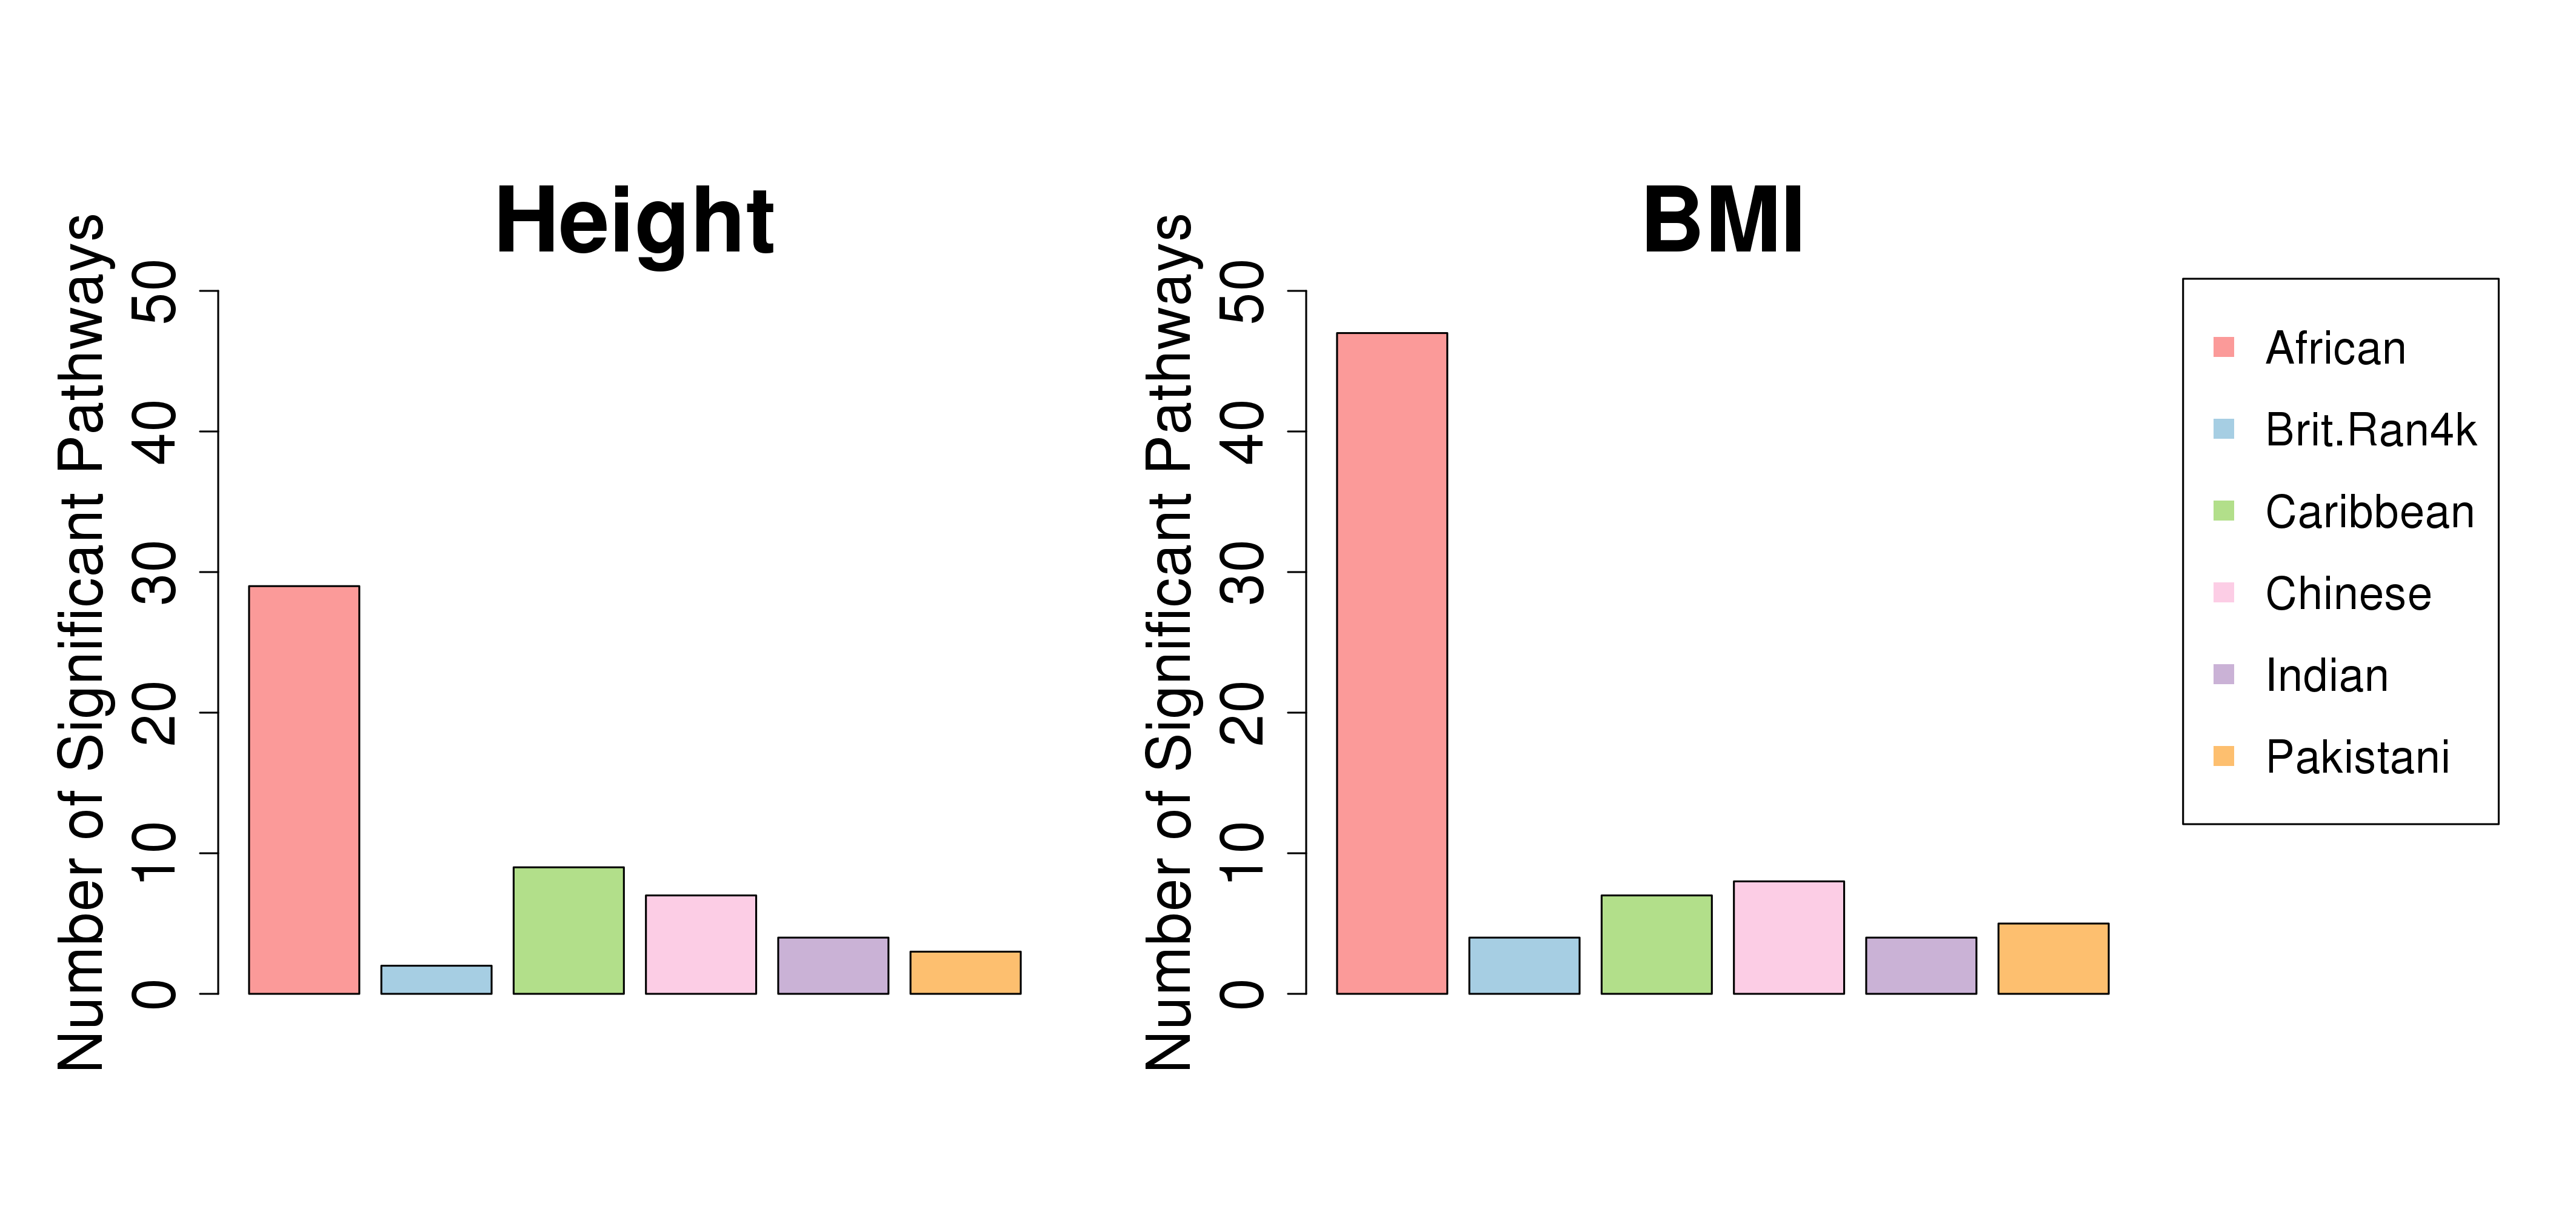
\includegraphics[scale=.45]{Images/Main/InterPath_Main_Figure_Barplots_KEGG_vs2.png}
\caption[TBD]{\textbf{Numbers of KEGG pathways that have significant marginal epistasis, per subgroup}. The figure shows the numbers of genome-wide significant pathways found from running MAPIT-R on height and BMI in the KEGG database within each of our UKB subgroups. Results from running MAPIT-R with REACTOME database pathways can be found in Supplementary Figure \ref{InterPath-Supp-Figure-Barplots-REACTOME}. Genome-wide significance was determined by using Bonferroni-corrected $p$-value thresholds based on the number of pathways tested in each phenotype, database, and subgroup combination. As shown in these results, we find across all phenotype and database combinations that the African subgroup has the largest numbers of significant pathways. For lists of the specific significant pathways per phenotype, database, and subgroup combination, see Supplementary Tables \ref{InterPath-Supp-Table-TopPathways-KEGG-Height-a}\textcolor{blue}{-d}.}
\label{InterPath-Main-Figure-Barplots-KEGG}
\end{figure}

This abundance of signal in the African subgroup stands out since the African subgroup is neither our subgroup with the largest sample size or our subgroup with the largest number of SNPs (Supplementary Table \ref{InterPath-Supp-Table-UKBPopStats}). However simulations done under a number of biological scenarios show MAPIT-R behaves properly under the null (Supplementary Figure XX). Additionally, we used permuted phenotypes as another check of MAPIT-R's behavior under the null, and we indeed find this to be the case (Supplementary Figures \ref{InterPath-Supp-Figure-perm1-QQPlots-AllPaths} and \ref{InterPath-Supp-Figure-10perms-pValHists}); we also used these permutations to investigate MAPIT-R's false discovery rates and observe values only as high as 1.5\% across our multiple phenotype, database, and subgroup combinations at different significance thresholds (Supplementary Table \ref{InterPath-Supp-Tables-AllPops-FDRs}).

\subsection{Non-African Subgroups also Identify Pathways that Contain Marginal Epistasis}

Expanding beyond the results from our African subgroup, we see 80 other pathways that are significant across the other subgroups. Many of these other pathways overlap with the set of significant results from the African subgroup, though there is less overlap between other non-African subgroups (Figure \ref{InterPath-Main-Figure-Heatplots-KEGG} \& Supplementary Figure \ref{InterPath-Supp-Figure-Heatplots-REACTOME}). For example, in the KEGG Height results the Caribbean subgroup overlaps with the African subgroup for 6 of its 7 pathways, and the Chinese subgroup overlaps with the African subgroup for 7 of its 8 pathways; however, there is no overlap between the Chinese and Caribbean subgroups. This continual overlap between the non-African subgroups and the African subgroup may suggest that the first sets of pathways to be identified as having marginal epistasis interactions will be widely important biologically, hence seeing themes such as cellular signaling and the immune system; identifying more population-specific examples of pathway-level marginal epistasis may require greater sample sizes. 

\begin{figure}[htb]
\centering
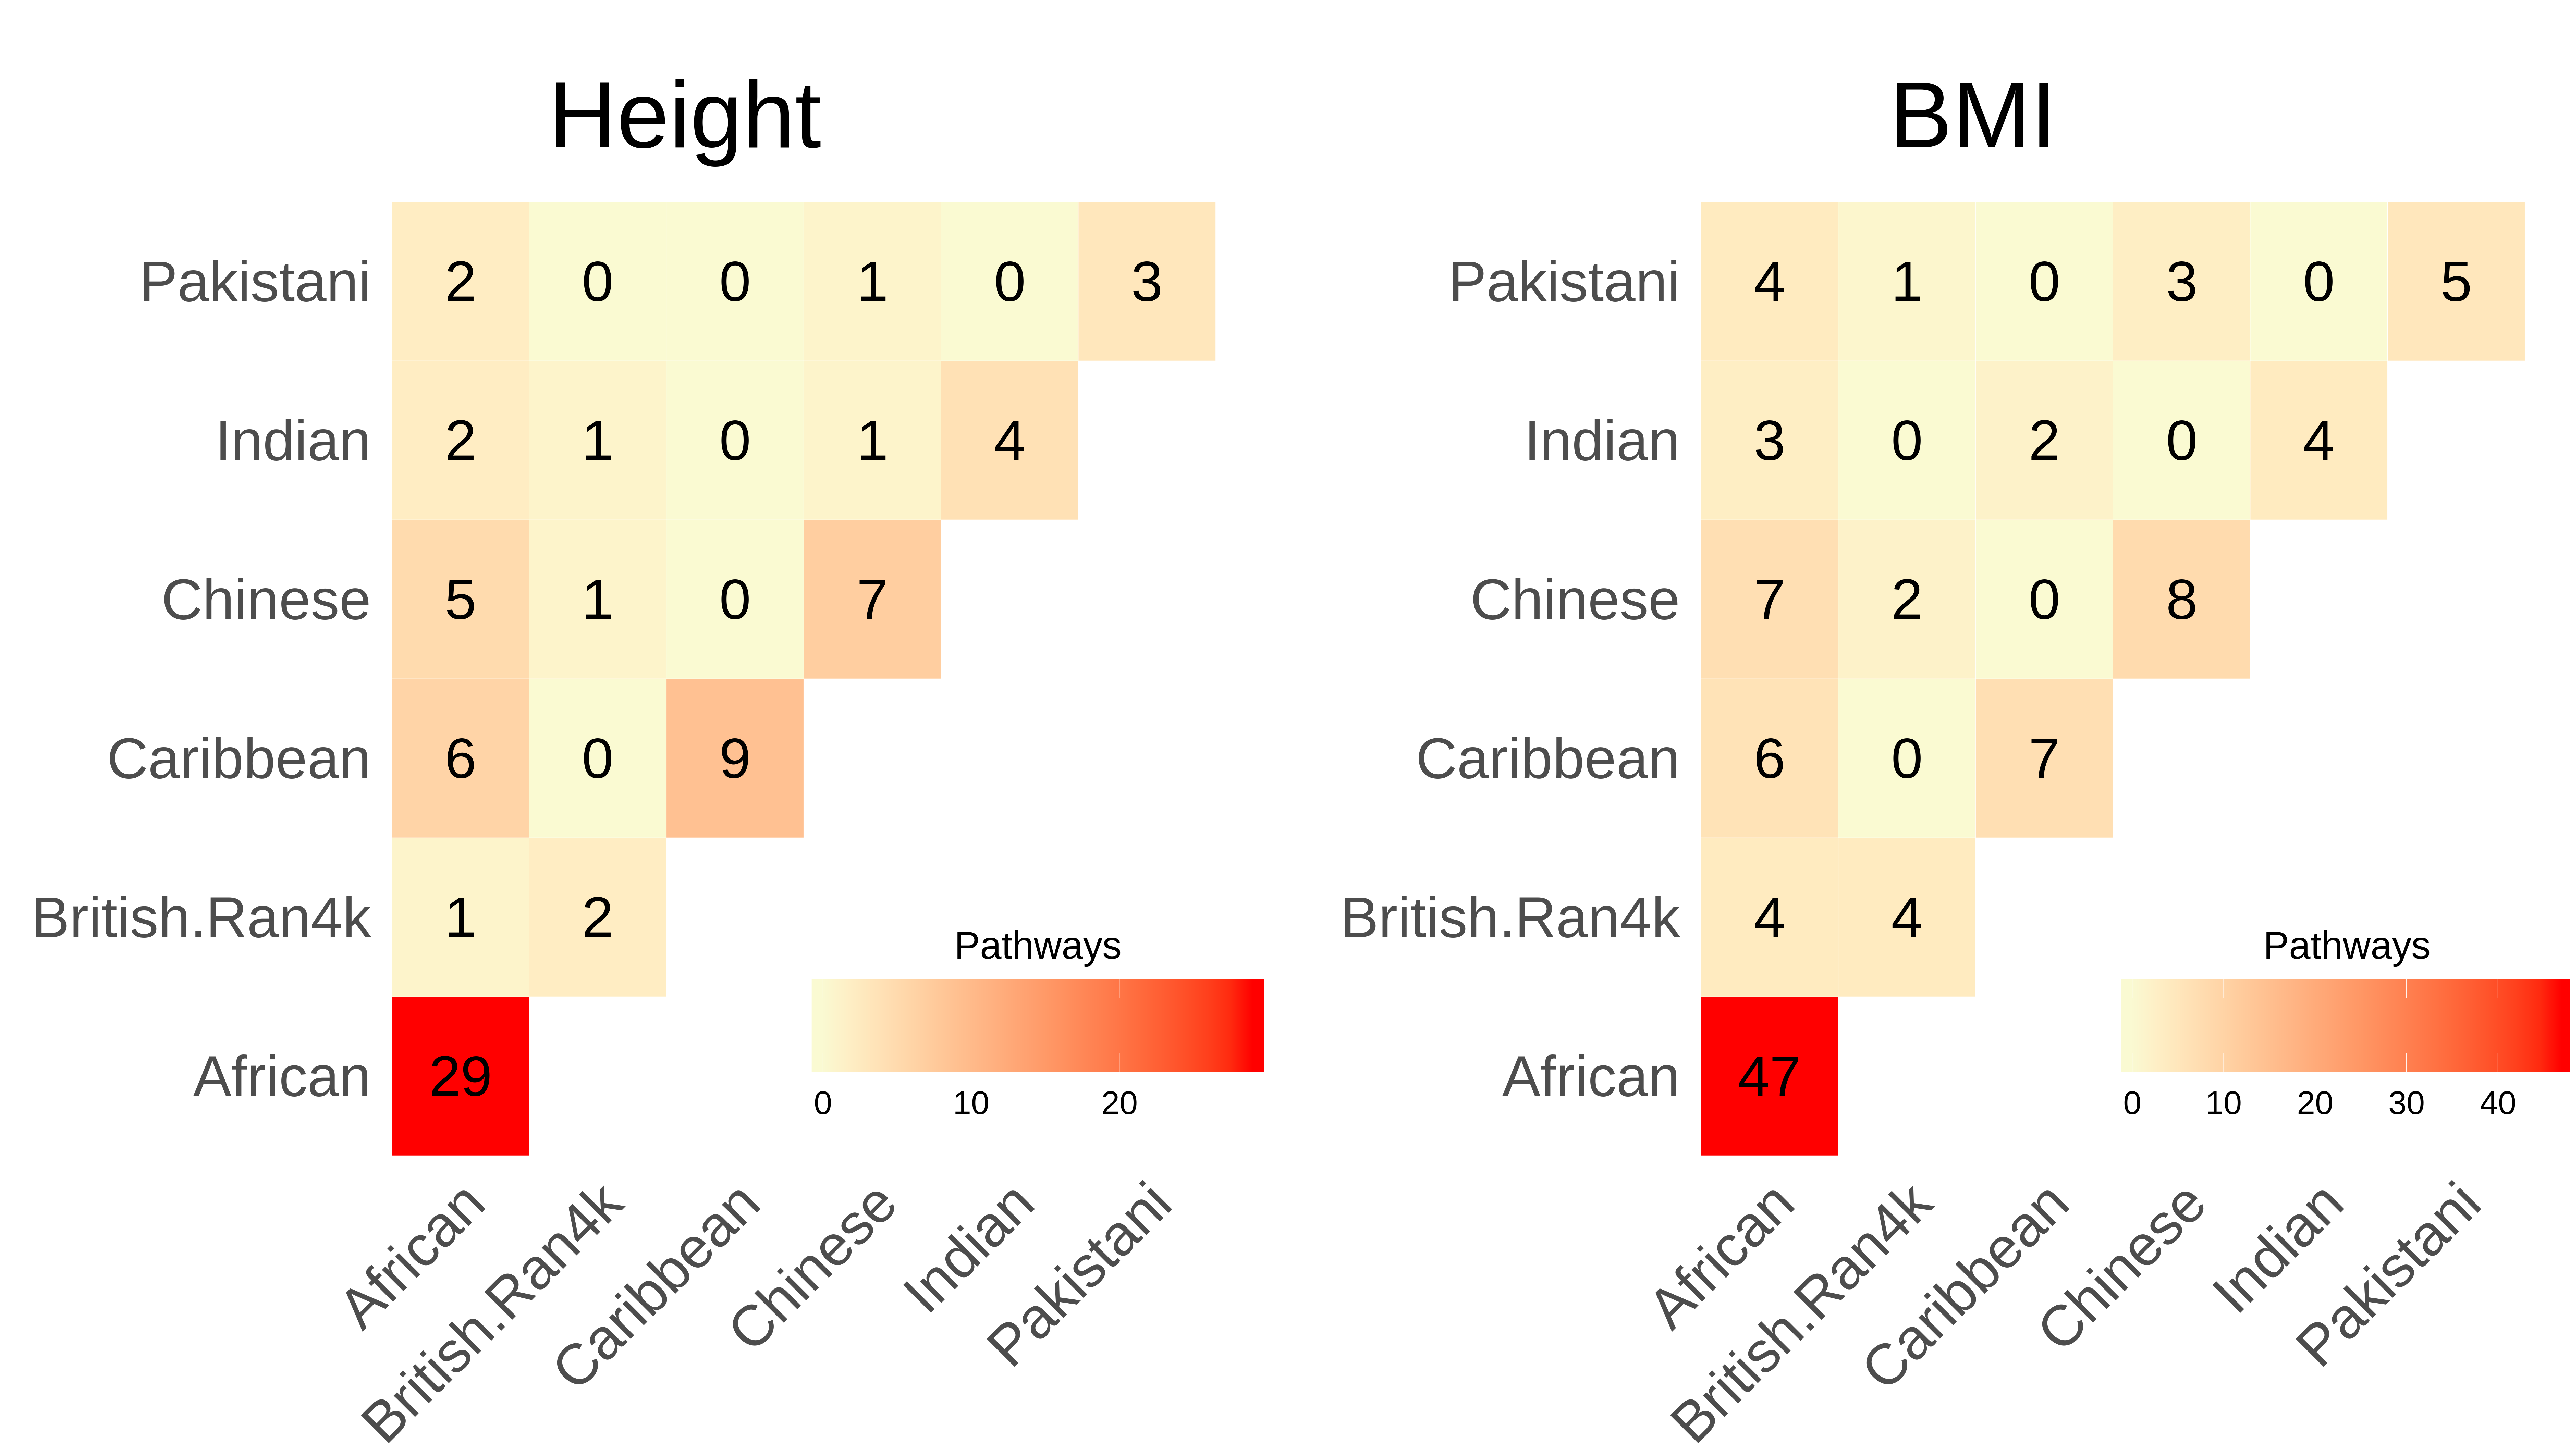
\includegraphics[scale=.225]{Images/Main/InterPath_Main_Figure_Heatplots_KEGG_vs2.png}
\caption[TBD]{\textbf{Overlap of MAPIT-R significant KEGG pathways between UKB subgroups}. The heatplots show the numbers of genome-wide significant MAPIT-R pathways that overlap between each UKB subgroup for height and BMI in the KEGG database. Results for both phenotypes in the REACTOME database can be seen in Supplementary Figure \ref{InterPath-Supp-Figure-Heatplots-REACTOME}. The diagonal shows the total number of genome-wide significant pathways per population subgroup. We observe that subgroups more frequently have overlap with the African subgroup than they do with the remaining non-African subgroups.}
\label{InterPath-Main-Figure-Heatplots-KEGG}
\end{figure}

Looking into the specific pathways in each of these overlaps, we find pathways related to the cellular signaling and heart condition patterns from before in the overlap between the African and Caribbean subgroups; additionally these overlaps appear to be driven by multiple kinases (eg MAPK1, ROCK1, PRKCB, PAK1) and calcium channel proteins (eg CACNA1S, CACNA1D) (Supplementary Tables \ref{InterPath-Supp-Tables-MAPITR-TopPathway-Overlap} \& \ref{InterPath-Supp-Tables-MAPITR-TopPathway-GeneCounts-Overlap}). The overlap between the African and Chinese subgroups however contain pathways related to the immune system and appear to be driven primarily by multiple HLA loci (eg HLA-DRA, HLA-DRB1, HLA-A, HLA-B) (Supplementary Tables \ref{InterPath-Supp-Tables-MAPITR-TopPathway-Overlap} \& \ref{InterPath-Supp-Tables-MAPITR-TopPathway-GeneCounts-Overlap}). These differences between ancestries may reflect heterogeneous power to detect epistatic signals. 

\subsection{BMI Contains Stronger Signals Than Height For Pathway-Level Marginal Epistasis}

Focusing again on the African subgroup, we observe in both the KEGG and REACTOME databases that BMI contains more significant pathways than height. While there is a strong correlation between height and BMI MAPIT-R -$\log_{10}$ $p$-values (.851 in KEGG and .858 in REACTOME), there is consistently more genome-wide significant pathways in BMI (Figure \ref{InterPath-Main-Figure-MAPITR-PhenoComps-African}). These results align with pedigree-based heritability estimates for each trait, which have indicated narrow-sense heritability is around .8 in height and between .4 and .6 in BMI \citep{Elks2012,Visscher2012}; overall these estimates suggest that non-additive effects may play a greater role in BMI than height, which is what we observe here. 

\begin{figure}[htb]
\centering
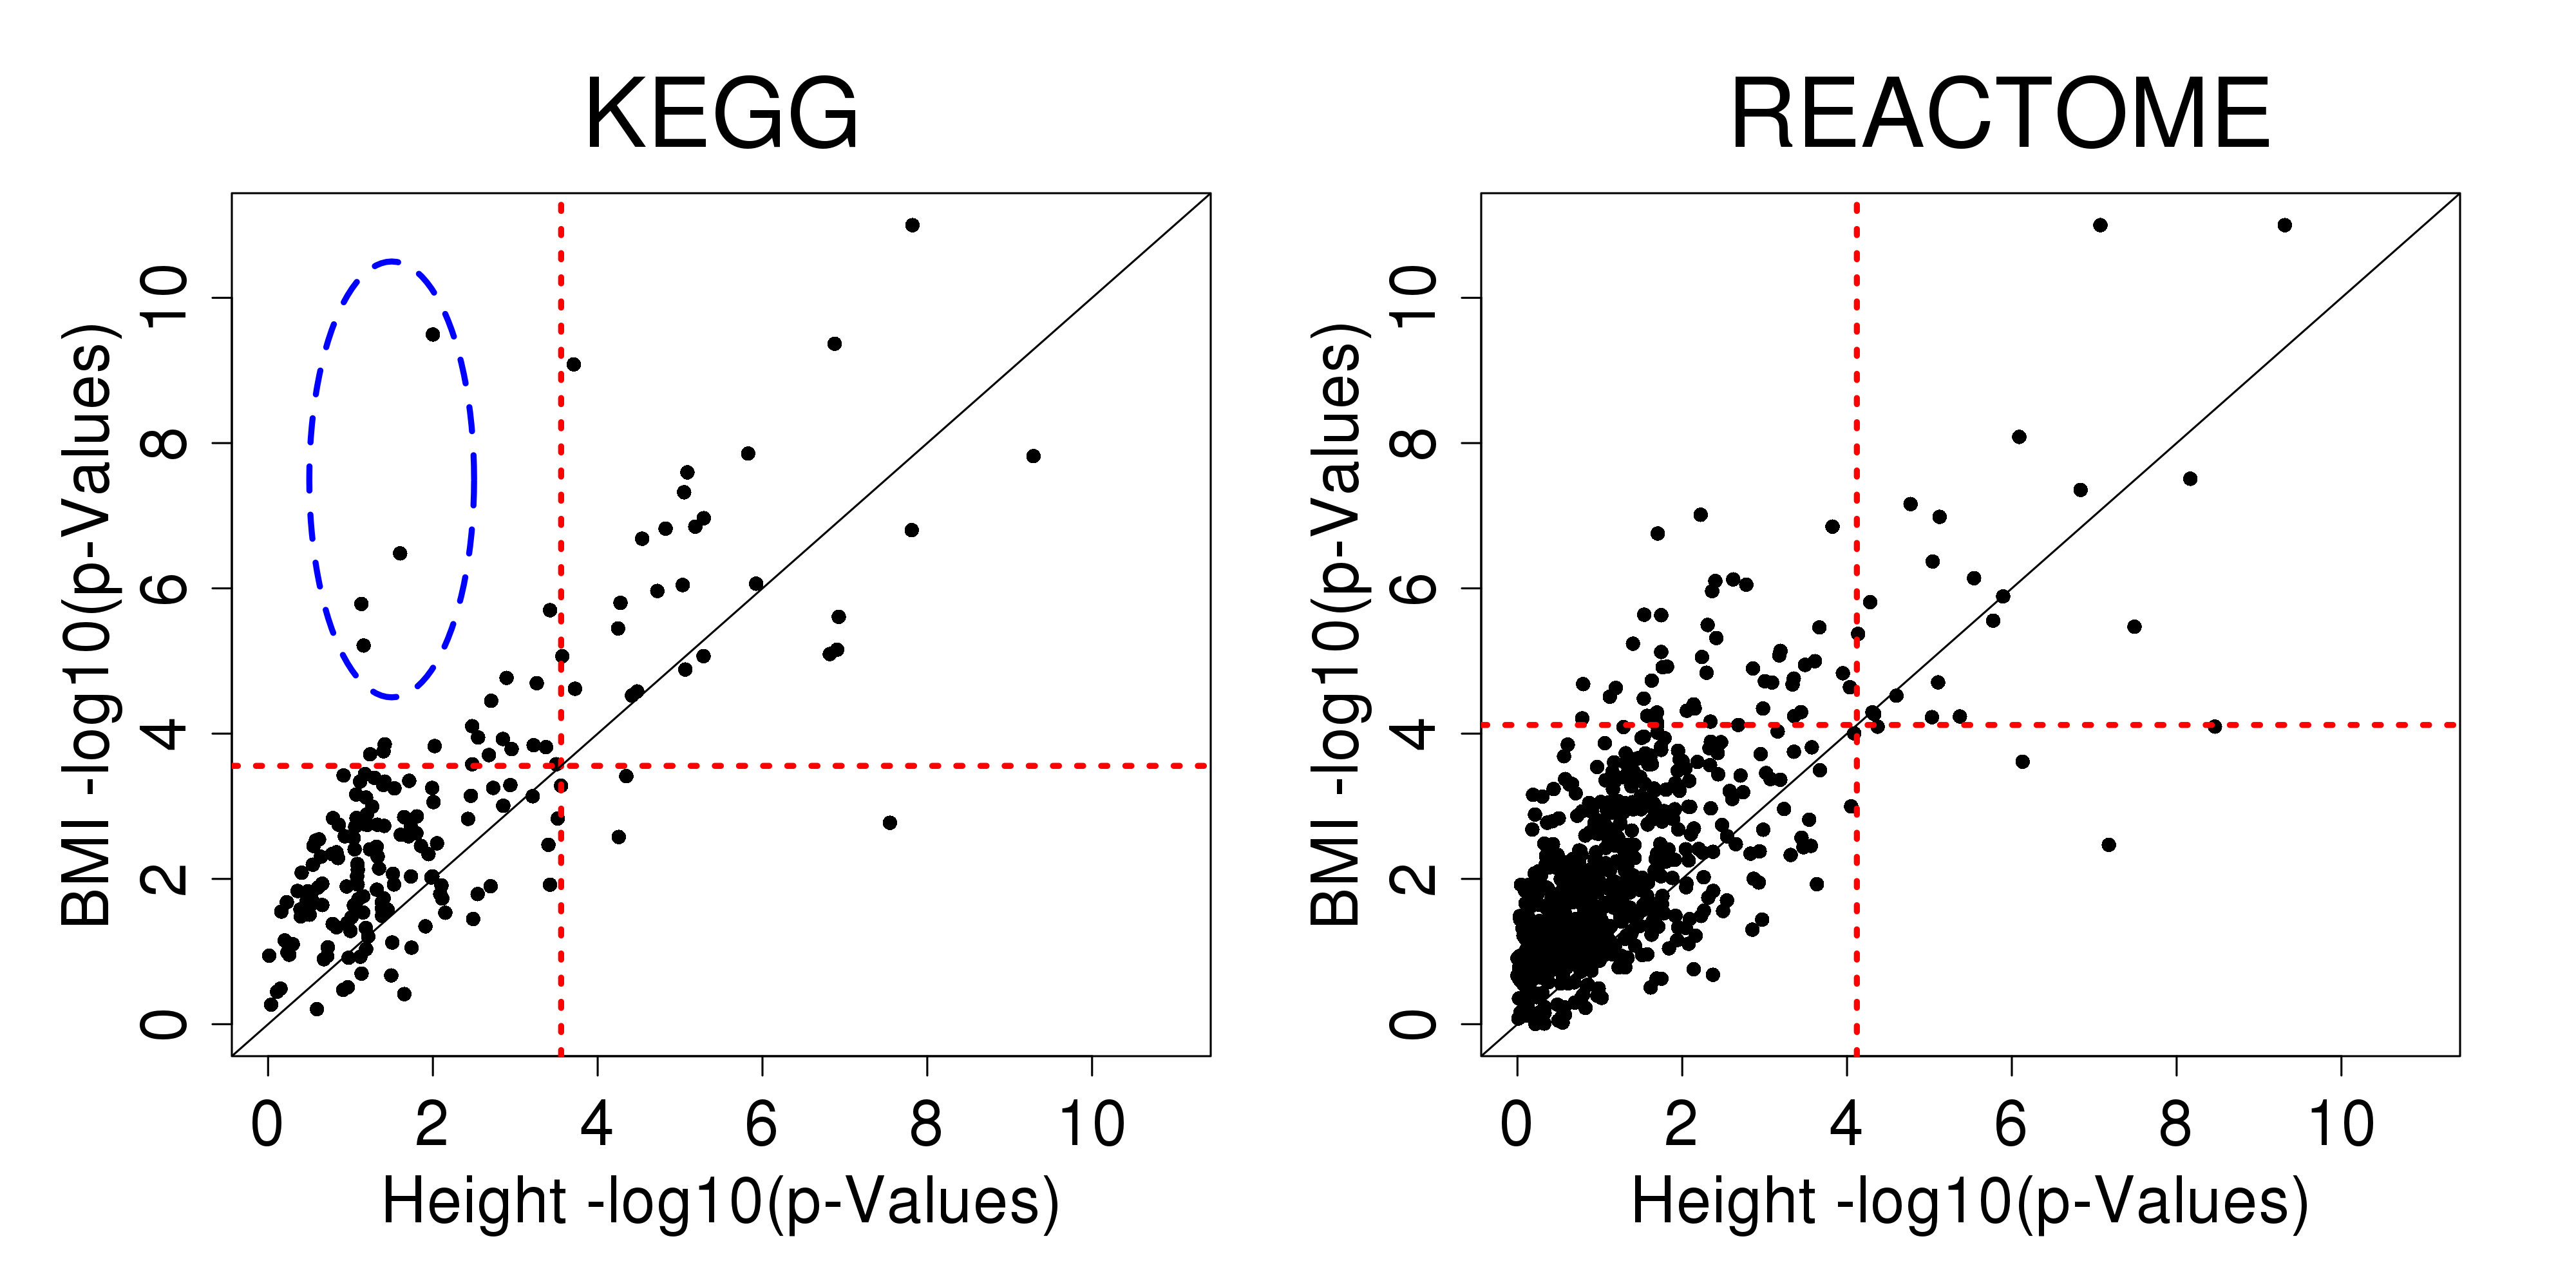
\includegraphics[scale=.45]{Images/Main/InterPath_Main_Figure_MAPITR_PhenoComps_African_vs3.png}
\caption[TBD]{\textbf{Comparison of MAPIT-R results between height and BMI in the African subgroup}. The figure shows MAPIT-R height results plotted against MAPIT-R BMI results for all pathways from the KEGG and REACTOME databases in the African subgroup. The $x$-axis is the MAPIT-R height -$\log_{10}$ $p$-value and the $y$-axis is the MAPIT-R BMI -$\log_{10}$ $p$-value. The dotted red lines are the Bonferroni-corrected $p$-value thresholds for genome-wide significance in each pathway and phenotype combination. The blue ellipse in the KEGG results highlight four pathways that appear to have much more significant BMI $p$-values than height $p$-values. In general though, across both databases, we see more significant $p$-values in BMI than height. For these comparisons in all the UKB subgroups, see Supplementary Figure \ref{InterPath-Supp-Figure-MAPITR-PhenoComps-AllPops}.}
\label{InterPath-Main-Figure-MAPITR-PhenoComps-African}
\end{figure}

Looking specifically at pathways that diverge in significance between height and BMI, we find one cluster of pathways in the KEGG results that separate out as particularly more significant in BMI than height. The four pathways circled in Figure \ref{InterPath-Main-Figure-MAPITR-PhenoComps-African}, sorted by decreasing -$\log_{10}$ $p$-value, are KEGG\_SMALL\_CELL\_LUNG\_CANCER, KEGG\_ERBB\_SIGNALING\_PATHWAY, KEGG\_NON\_SMALL\_CELL\_LUNG\_CANCER, and KEGG\_T\_CELL\_RECEPTOR\_SIGNALING\_PATHWAY. We once again see a theme of signaling pathways, but now also a trend of oncogenic pathways. Looking at the genes driving these pathways (Supplementary Table \ref{InterPath-Supp-Table-MAPITR-PhenoComps-African-GeneCounts}), we find two sets of gene families that appear in all four pathways: phosphatidylinositol 3-kinases (PIKs) and the AKT serine/threonine-protein kinases. One gene that stands out from this group is AKT2, a locus that has been associated with multiple monogenic disorders of glucose metabolism, including severe insulin resistance and diabetes, and severe fasting hypoinsulinemic hypoglycemia \citep{George2004,Manning2017,Latva-Rasku2018}. This gene may have more marginal epistatic interactions relevant to BMI than height then, possibly being a driver for this pathway cluster.

\subsection{The Proteasome is Enriched for Marginal Epistatic Interactions}

With a large number of pathways now identified as being impacted by marginal epistasis, we wanted to identify possible biological mechanisms or processes that were driving these results. One approach to do this is to see whether any genes are significantly represented among the genome-wide significant pathways we identified versus the background distribution of pathways in each database. To accomplish such an analysis, we ran hypergeometric tests for enrichment to identify whether any genes were significantly over-represented among our significant pathways. 

And indeed, by doing so, we find many genes that are significantly enriched among our significant MAPIT-R pathways (Supplementary Figure \ref{InterPath-Supp-Figure-Hypergeometric-QQPlots-African}). In the African subgroup for example, we find an abundance of `significant' $p$-values for both height and BMI in both pathway databases. Using the conservative Bonferroni cutoff of $2.082\times10^{-5}$ (.05 / 2401 genes), we would identify 45 genes as being significantly enriched in the REACTOME BMI analysis. However, one possible confounder to our analysis is that pathways with more genes, and therefore more variants, are more likely to have smaller MAPIT-R $p$-values (Supplementary Figure \ref{InterPath-Supp-Figure-pValsVsNumSNPs}); this follows our original hypothesis that analyzing multiple variants should lead to more power to detect associations (though we note that solely having more variants does not lead to smaller MAPIT-R $p$-value, as shown in the permuted phenotype analyses; Supplementary Figure \ref{InterPath-Supp-Figure-pValsVsNumSNPs-perm1})\footnote{\textcolor{blue}{MT: should this, bringing up the permutation results, be a comment in the caption of the supplementary figure and not something brought up in the main text?}}. As a result, this enrichment analysis may be moreso identifying genes that are overrepresented among larger pathways, such as housekeeping genes, than genes that are necessarily overrepresented among MAPIT-R significant pathways. 

To limit the effect of this possible confounder, we reran our enrichment analysis, but this time only using pathways with less than 1,000 SNPs. And indeed, we see a large drop in the number of genes that are significantly enriched among our significant, but smaller, MAPIT-R pathways; most subgroups no longer have any significant genes, and the African subgroup has many fewer significant genes (29 to 2 in KEGG height, 47 to 11 in KEGG BMI, 24 to 0 in REACTOME height, and 65 to 26 in REACTOME BMI; Figure \ref{InterPath-Main-Figure-Hypergeometric-RestrictedComps-African-BMI}). However, we do also see one gene and a separate gene family  have experienced the opposite effect: their enrichment $p$-values have become more significant. The gene that has had the largest increase in significance is SMC3, a component of the multimeric cohesin complex. However, while having not as large a change in $p$-value, the next genes that experienced an increase in significance are all from the same family of proteins, the various subunits of the proteasome complex (PSMA*, PSMB*, PSMC*, PSMD*, PSME*, and PSMF*). The proteasome is one half of the ubiquitin-proteasome system (UPS), a critical system for a variety of processes related to protein degradation within the cell \citep{Voges1999,Livneh2016,Collins2017}. Whereas ubiquitin is the first half of this system that tags proteins for eventual degradation, the proteasome is the second half of this system that catalyzes the degradation itself. The main proteasome isoform, 26S, is made up of two main components: the 20S main core of four stack rings (an outer, structural ring encoded by PSMA genes, and an inner, catalytic ring encoded by PSMB genes) and the 19S regulatory caps which booked both sides of the main core (encoded by both PSMC and PSMD genes) (Figure \ref{InterPath-Main-Figure-Proteasome-Schematic}). For our purposes of investigating marginal epistasis, the proteasome offers a unique opportunity to not only further refine the original pathway-level signal, but also to further show the utility of group-based approaches.

\begin{figure}[htbp]
\centering
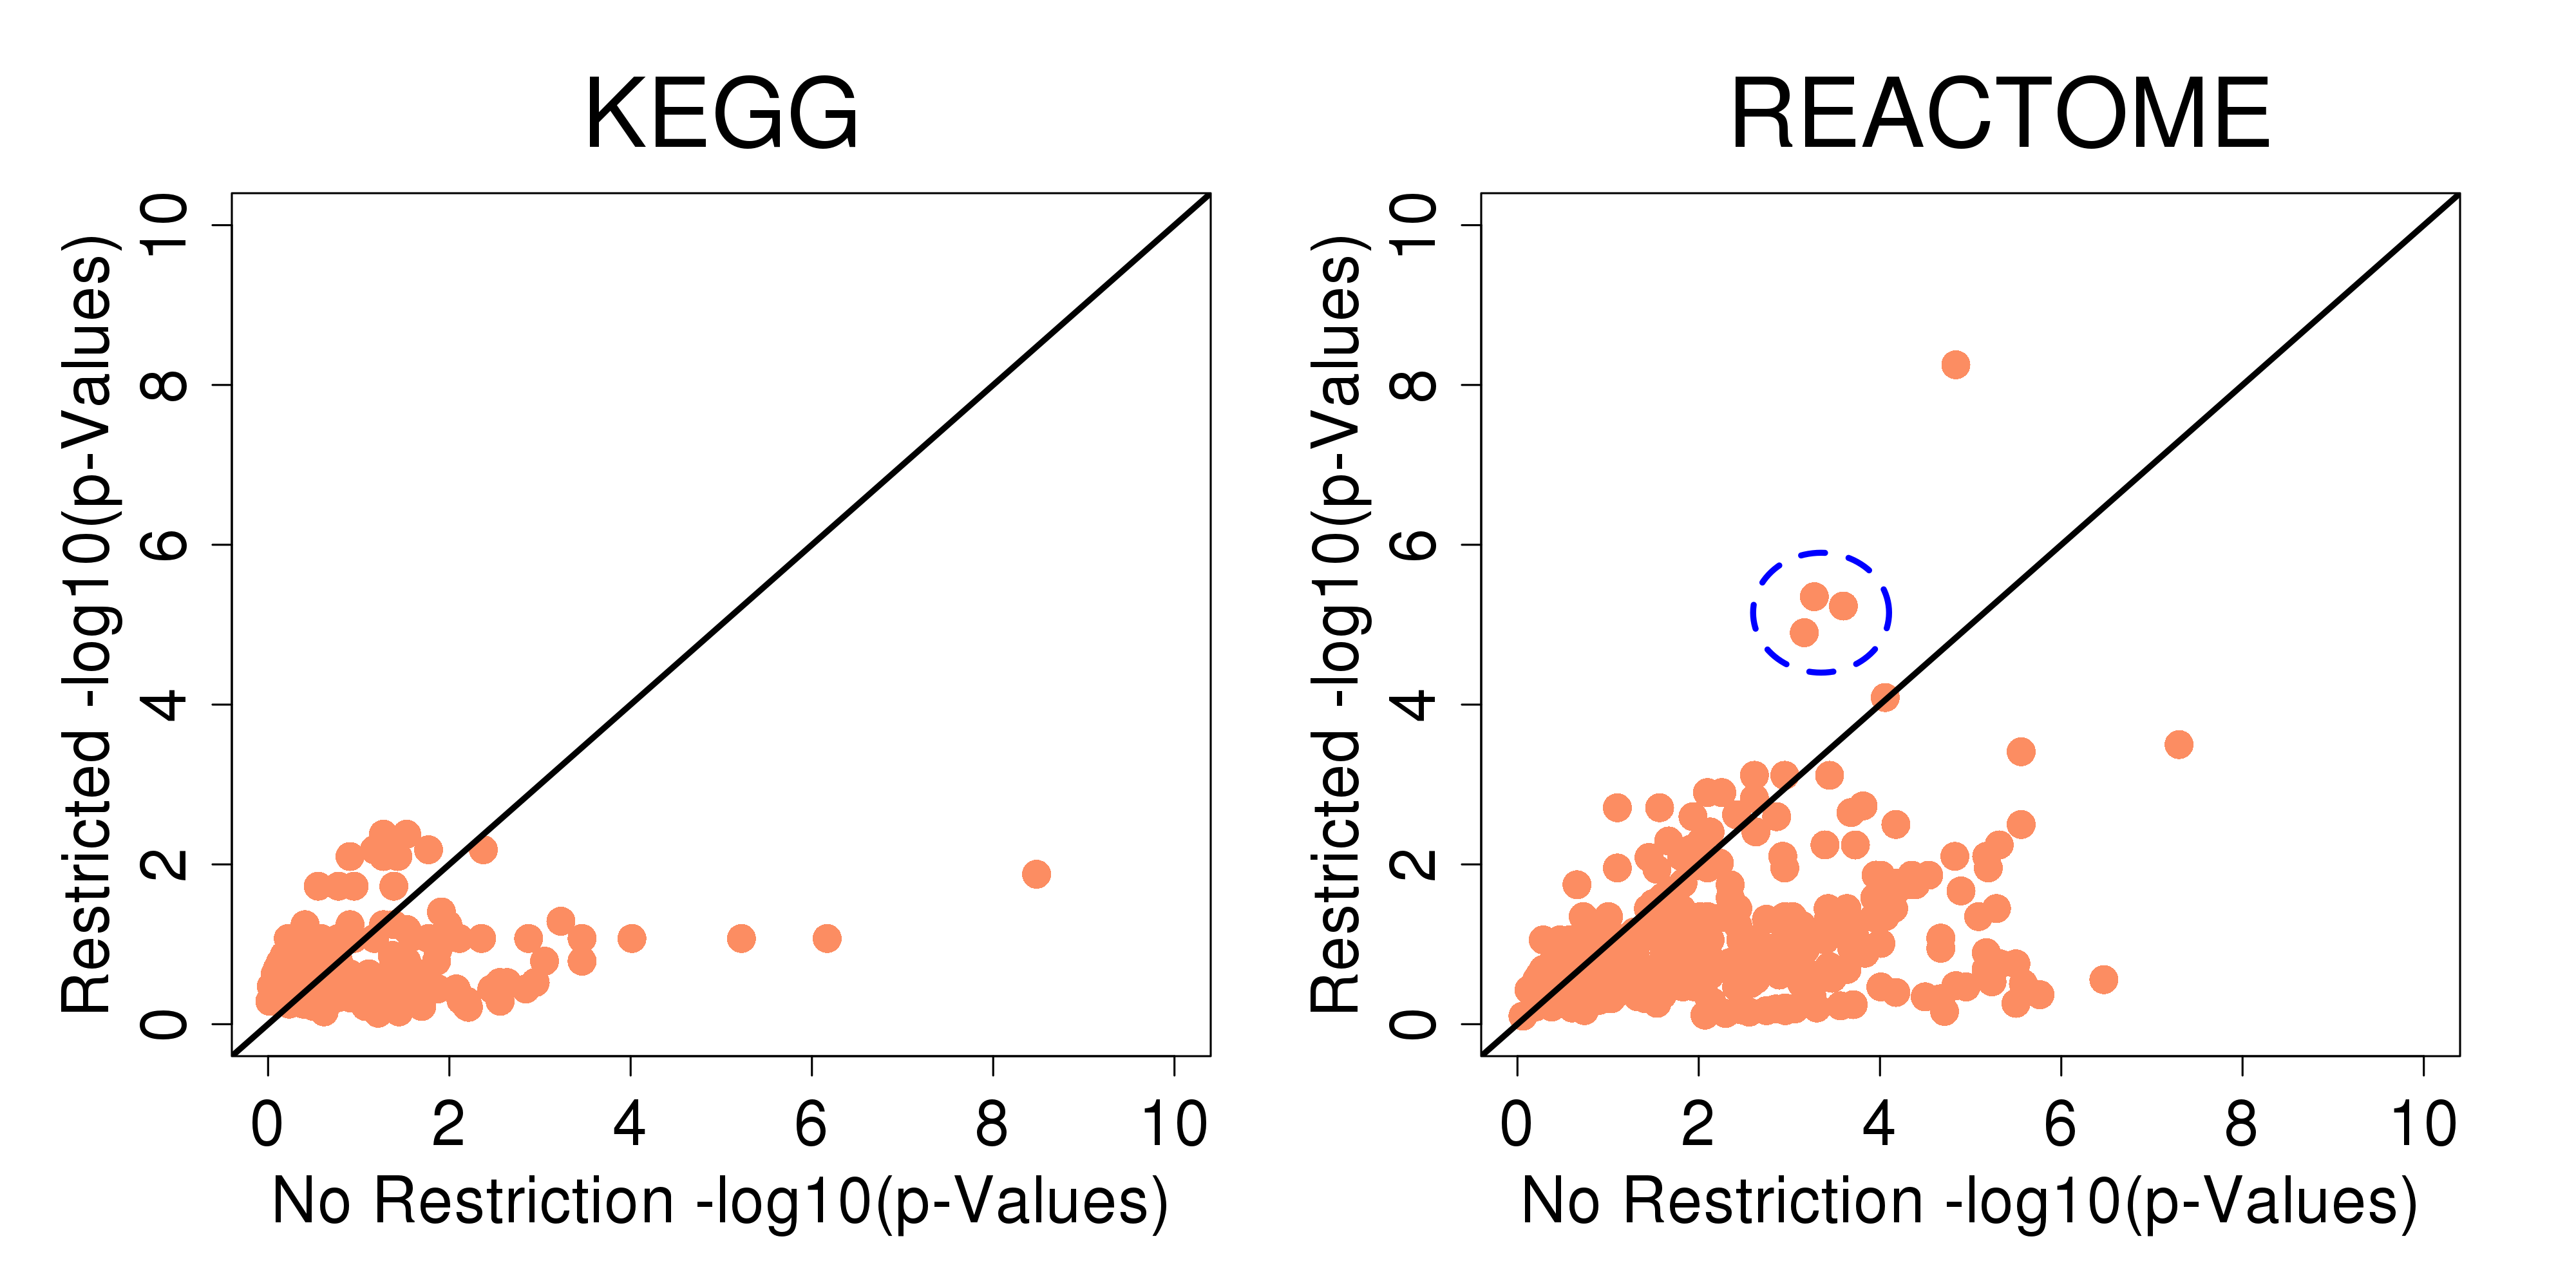
\includegraphics[scale=.4]{Images/Main/InterPath_Main_Figure_Hypergeometric_RestrictedComps_African_BMI_vs2.png}
\caption[TBD]{\textbf{Comparison of gene count hypergeometric enrichment $p$-values in BMI using pathway size restrictions versus no size restrictions in the African subgroup}. The figure shows comparisons of the gene count hypergeometric enrichment $p$-values between the size restricted version of the analysis and the original unrestricted version of the analysis. The size restricted version of the analysis is redoing the hypergeometric enrichment tests but only using pathways that contained $<$ 1,000 SNPs. Only results for BMI are shown here since almost all Bonferroni significant pathways were lost in the height results due to this size restriction step. The $x$-axis shows the original, unrestricted hypergeometric -$\log_{10}$ $p$-values, and the $y$-axis shows the new, size restricted hypergeoemtric -$\log_{10}$ $p$-values. The PSM* gene cluster is highlighted in the REACTOME plot. For lists of the top genes that became more significant due to the size restriction step, see Supplementary Table \ref{InterPath-Supp-Table-Hypergeometric-RestrictedComps-African-BMI-TopExamples}.}
\label{InterPath-Main-Figure-Hypergeometric-RestrictedComps-African-BMI}
\end{figure}
\clearpage

\begin{figure}[htb]
\centering
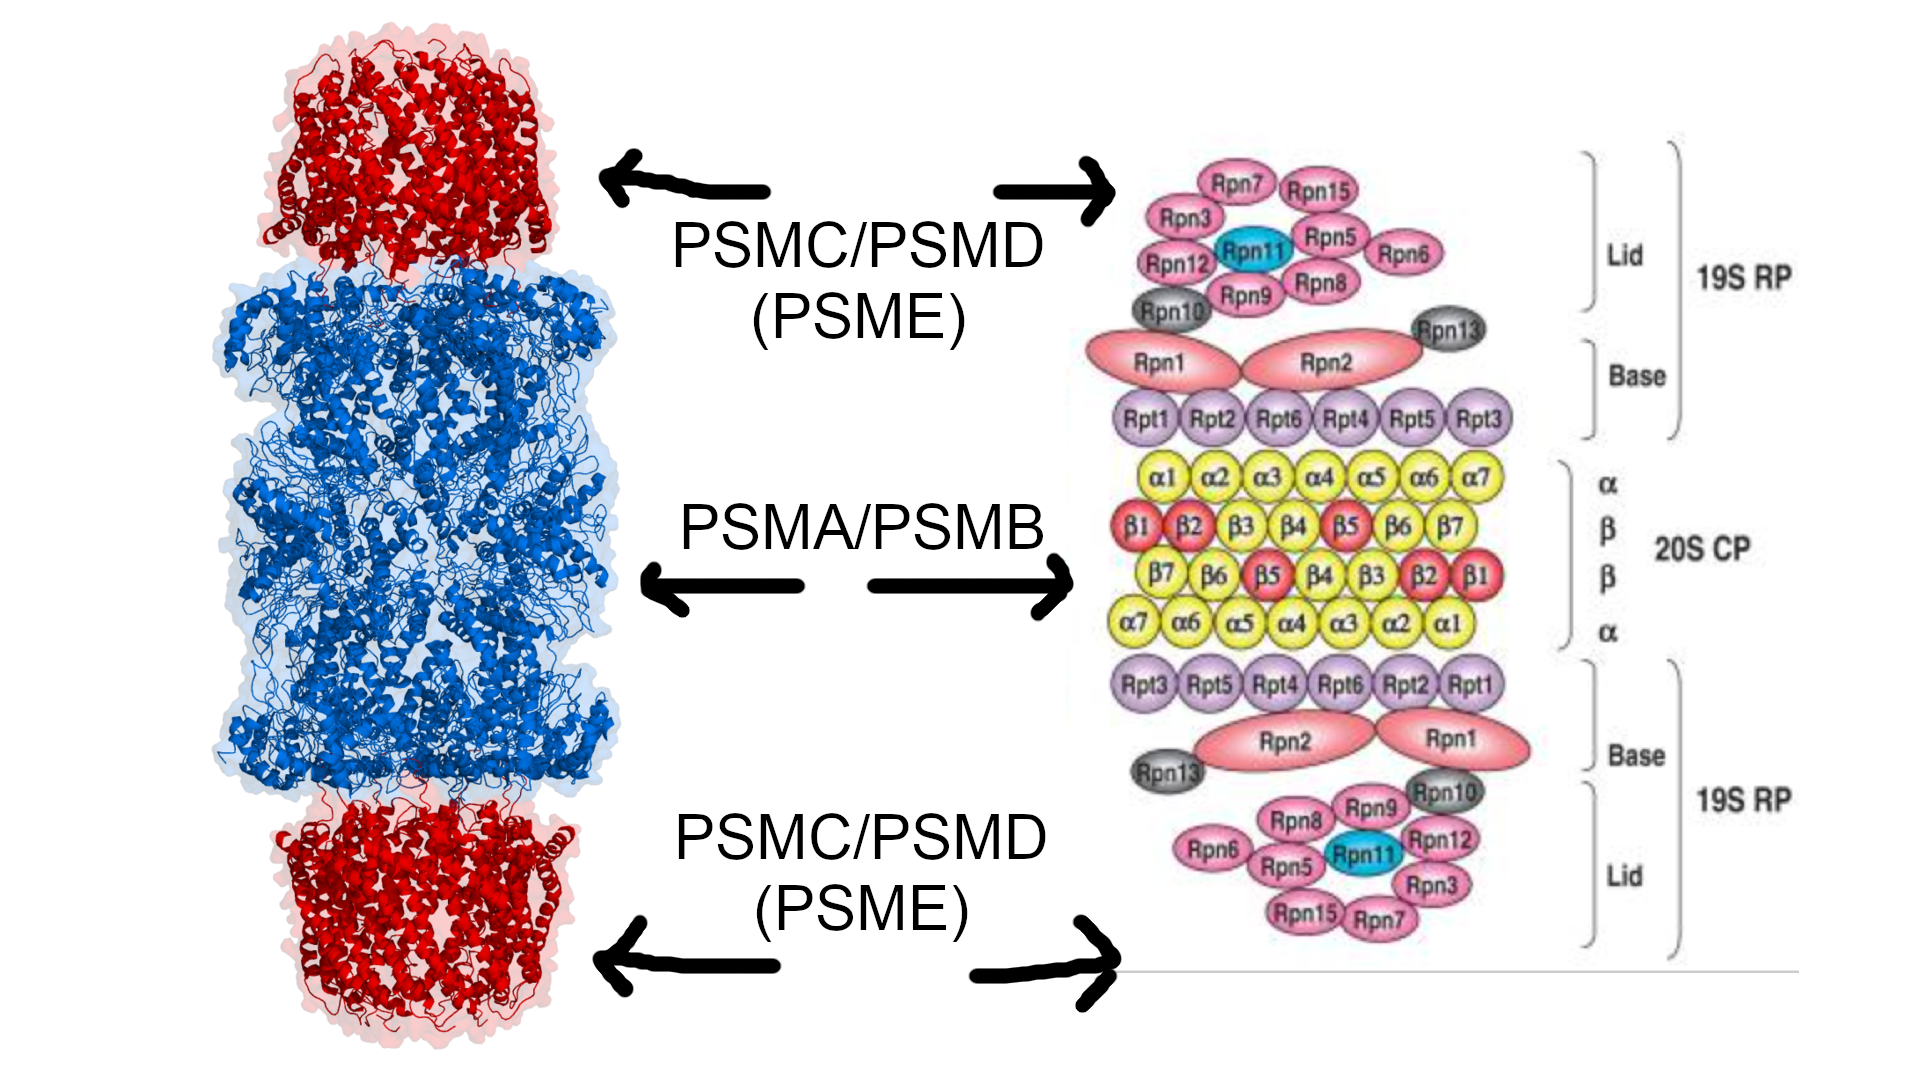
\includegraphics[scale=.2]{Images/Main/MockUp1.png}
\caption[TBD]{\textbf{Structure of the Proteasome}. The figure shows the different components of the proteasome and which gene families encode which part. \textcolor{blue}{MT: currently a mockup of an idea on how to present this -- maybe this and the heatplot should be one larger figure? }
}
\label{InterPath-Main-Figure-Proteasome-Schematic}
\end{figure}

Specifically, we were interested in determining whether any subunit of the proteasome is particularly enriched for marginal epistasis compared to the rest of the subunits. To investigate this, we can create versions of the original pathways analyzed where each individual subunit has been removed; in turn this could reveal whether any particular subunit leads to much greater loss in MAPIT-R $p$-value than compared to the other subunits. Therefore, we reran each genome-wide significant MAPIT-R pathway that contained these proteasome subunit gene families and incrementally ran pathway versions with each subunit gene family removed. We ran these analyses specifically in the African subgroup and BMI since this combination is where the original signal was strongest. 

And indeed we observe that some proteasome subunits appear to have greater impacts on the original MAPIT-R pathway $p$-values than others (Figure \ref{InterPath-Main-Figure-Proteasome-Heatplot}). In particular, the patterns involving the PSMA and PSME gene families stand out. First, genes from the PSME family encode an alternative regulatory cap (11S or PA28) that can also associate with the main 20S core; this hybrid-proteasome is part of a subset of isoforms known as immunoproteasomes. Immunoproteasomes are specialized proteasomes that are expressed at higher levels in hematopietic cells and are more directly associated with immunity-related processes such as MHC antigen presentation \citep{Ferrington2012,Basler2013,McCarthy2015}. PA28 itself is an Interferon-$\gamma$ (IFN-$\gamma$) inducible isoform that operates in a ubiquitin-independent manner, increasing production of a specific subset of MHC-1 presenting antigens \citep{Groettrup1996,de2011,Raule2014,Murata2018}. Additionally, recent work has more directly connected PSME genes as potential upregulators of NF$\kappa$B as well \citep{Sun2016,Mitchell2019}. Therefore this may explain why removal of the PSME gene family produces larger drops than other subunits in the MAPIT-R $p$-values of pathways related to NF$\kappa$B, B-cells, HIV-infection, and apoptosis. Second, genes from the PSMA family encode the outer two rings of the core four in the 20S structure. These outer, `alpha' rings are gates which help control the entry of proteins into the core of the proteasome. Unlike the regulatory caps or the inner `beta' rings (encoded by the PSMB family), which contain protease active sites, the outer rings have no known catalytic functionality, which is what may be reflected by the consistent lack of change in MAPIT-R $p$-values across each pathway when PSMA genes are removed. In some instances it appears that removing PSMA genes may even improve MAPIT-R $p$-values. Therefore in two instances we see examples of how biological function may align with observed impacts on pathway-level marginal epistasis signals.

%...is Interferon-$\gamma$ (IFN-$\gamma$) inducible and...

\begin{figure}[]
\centering
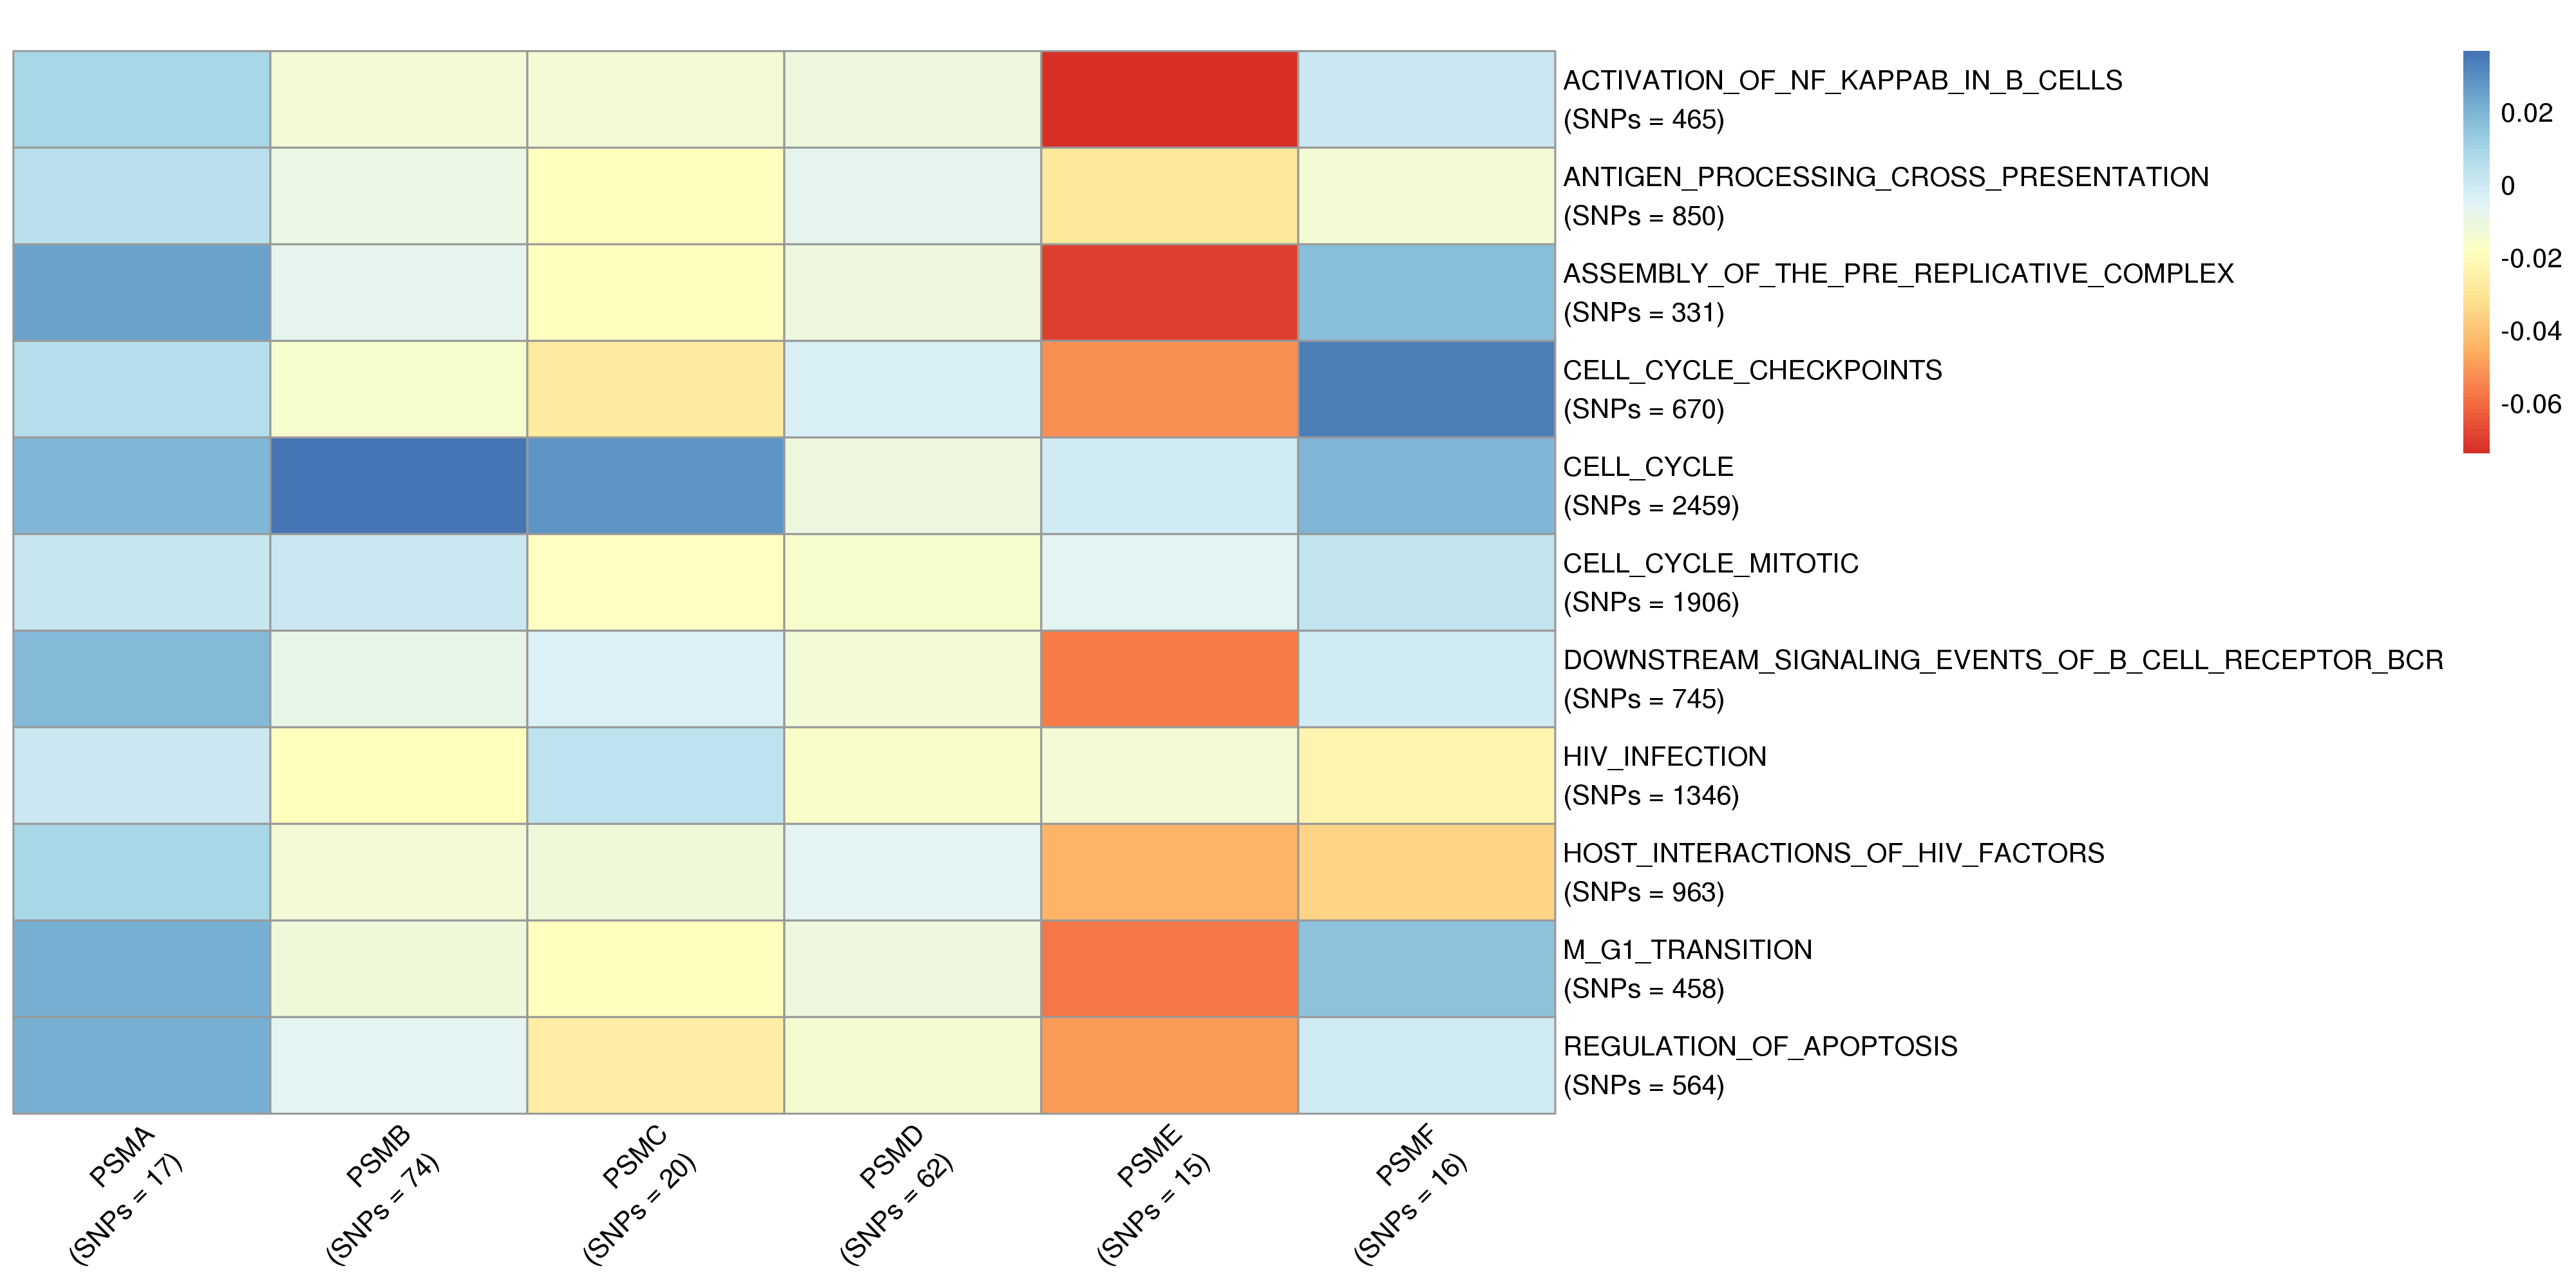
\includegraphics[scale=.45]{Images/Main/InterPath_Main_Figure_Proteasome_vs1.png}
\caption[TBD]{\textbf{Change in MAPIT-R $p$-values when removing proteasome subunits}. The figure shows how much the MAPIT-R $p$-value drops for each REACTOME pathway specified when all the SNPs mapping to each proteasome subunit gene family is removed from the analysis. Specifically the heatplot shows the -$\log_{10}$ $p$-value change per SNP, so each column is corrected for the number of SNPs that mapped to each subunit gene family. While we observe different $p$-value change patterns for every subunit gene family, we find that two patterns potentially align with biological function \textcolor{blue}{(MT: do you think we should add these kinds of details to this caption in particular?)}. First, removing the PSMA gene family appears to rarely have a negative impact on MAPIT-R $p$-values. PSMA genes also encode for the outer structural rings of the 20S structure and do not have any known catalytic activity, supporting they may have less important genetic interactions. Second, the PSME gene family appears to have particularly strong effects on pathways related to NF$\kappa$B, B-cells, HIV-infection, and apoptosis. PSME genes encode an alternative regulatory particle (11S or PA28) that can form hybrid-proteasome structures that are known to enhance production of a specific subclass of MHC-1 antigens in a ubiquitin-independent manner, and recent work has connected PSME genes to upregulation of NF$\kappa$B. Therefore PSME genes may have a different and stronger set of genetic interactions within these pathways as compared to the other subunit gene families, which is getting represented here.
}
\label{InterPath-Main-Figure-Proteasome-Heatplot}
\end{figure}

\subsection{MAPIT-R Provides Greater Evidence for Epistasis Than Single-SNP Methods in UKB Subgroups}\label{InterPath-Results-SNPEpistasis}

Part of our initial hypothesis was that testing multiple variants at once would provide greater power to detect marginal epistasis than testing only single variants. While we have now identified pathways with genome-wide significant signals of marginal epistasis, we wanted to investigate whether any of these signals, in particular the differences between ancestry subgroups, were identifiable on the single-SNP level. So to explore this, we applied MAPIT to each of our UKB subgroups for both height and BMI. We find that there are no SNPs with genome-wide significant signals for marginal epistasis ($p$-value $< 5\times10^{-8}$; Supplementary Figure \ref{InterPath-Supp-Figure-MAPIT-HeightBMI}). While we observe possible enrichment of marginally significant $p$-values ($p$-value $< 5\times10^{-4}$) in the African, Caribbean, and Indian subgroups versus the British, Chinese, and Pakistani subgroups in both phenotypes, it is not as clear a between-ancestry pattern as we observe in the MAPIT-R results. And to compare against the more typical, direct pairwise variant epistasis analysis, we also applied PLINK's exhaustive pairwise epistasis test \citep{Purcell2007} to each of our ancestry subgroups in height and BMI, and once again do not observe any genome-wide significant tests ($p$-value $\leq 5\times10^{-13}$, Bonferroni-corrected for $1\times10^{11}$ tests; Supplementary Figure \ref{InterPath-Supp-Figure-PLINK-HeightBMI-AllPops}). Overall analyzing groups of variants jointly with MAPIT-R provides a greater ability to detect epistasis in these UKB subgroups than using single variant methods. 

\subsection{Testing the Null Model with British Replicate Subpopulations}

One important consideration of our results is that we have limited representations of the different human ancestries we are analyzing. Are the samples we are analyzing large enough to be representative of the true total populations? While it is still difficult to address that question directly for non-European populations due to the limited availability of other public datasets, we are able to ask that question for the British ancestry subgroup. Specifically, we can take additional, non-overlapping random subgroups of 4,000 British individuals and see if they are at least consistent in their lack of results as compared to the original random subgroup. Furthermore, given the data availability, we also constructed sets of larger British subsamples to investigate the impact of sample size on our results as well. In total we analyzed 5 sets of 4,000 British individuals and 5 sets of 10,000 British individuals. 

And overall we see similar results across all replicates to our original results from the first set of 4,000 British individuals. We see limited numbers of significant pathways across all phenotype, database, and replicate subgroup combinations, as well as limited overlap of significant pathways between replicates (Supplementary Figures \ref{InterPath-Supp-Figure-BritReps-Barplots}\textcolor{blue}{-13}). We also ran analyses using permuted phenotypes, as before, and once again see proper behavior under the null and very low FDRs (Supplementary Tables \ref{InterPath-Supp-Tables-BritReps-FDRs-pt1}). While not presenting new significant pathways, these results at least suggest that the large numbers of significant pathways we observe in the African subgroup are less likely to be a product of simply choosing a particularly optimal set of individuals by chance.  

\subsection{Investigating the Relationship Between Within-Subgroup Genetic Variation and Detecting Epistasis}

As observed previously, the African subgroup produces the majority of our significant MAPIT-R pathways; a follow up question then is why we see such between-ancestry subgroup differences in our MAPIT-R results. One possibility is this reflects the amount of genetic variation present in each subgroup -- greater levels of genetic variation may allow for greater numbers of possible genetic interactions. It is also well-established that African-ancestry populations contain the highest levels of within-population genetic variation on average compared to other global populations \citep{International2010,Genomes2015,Mallick2016}. Therefore, we decided to investigate whether there were any connections between measures of genetic variation within and between our subgroups and the number of significant MAPIT-R pathways each subgroup produced.

Our first approach was to look at genome-wide levels of genetic variation both between and within our subgroups. To do this, we calculated both pairwise F\textsubscript{ST} values between every UKB subgroup as well as within population F\textsubscript{ST} values as well (Figure \ref{InterPath-Main-Figure-Fst}). For between subgroup F\textsubscript{ST}, we find values as large as .124, which are within range of previous global sample estimates \citep{Ramachandran2005,Weir2005,Wang2012,Sugden2016}. We find that while the African subgroup does have some of the largest divergences from other populations (such as versus the British subgroup), we also observe close to similar levels of divergence between the Chinese subgroup and other populations as well. However, looking at within subgroup F\textsubscript{ST} (the diagonal)\footnote{\textcolor{blue}{MT: note, this is predicated on using a proper metric for the diagonal; if we one doesn't come up, or if it doesn't match the following descriptions, I'll update things to match and follow the figure properly}}, we observe that the African subgroup has the largest amount of differentiation as compared to any other subgroup. Additionally, the Caribbean and Chinese subgroups are the subgroups with the next largest values of within subgroup F\textsubscript{ST}, approximately matching the order in which subgroups produce significant pathway MAPIT-R results. Therefore, we decided to look further into whether within subgroup levels of genetic variation are connected to more significant MAPIT-R results.

\begin{figure}[htb]
\centering
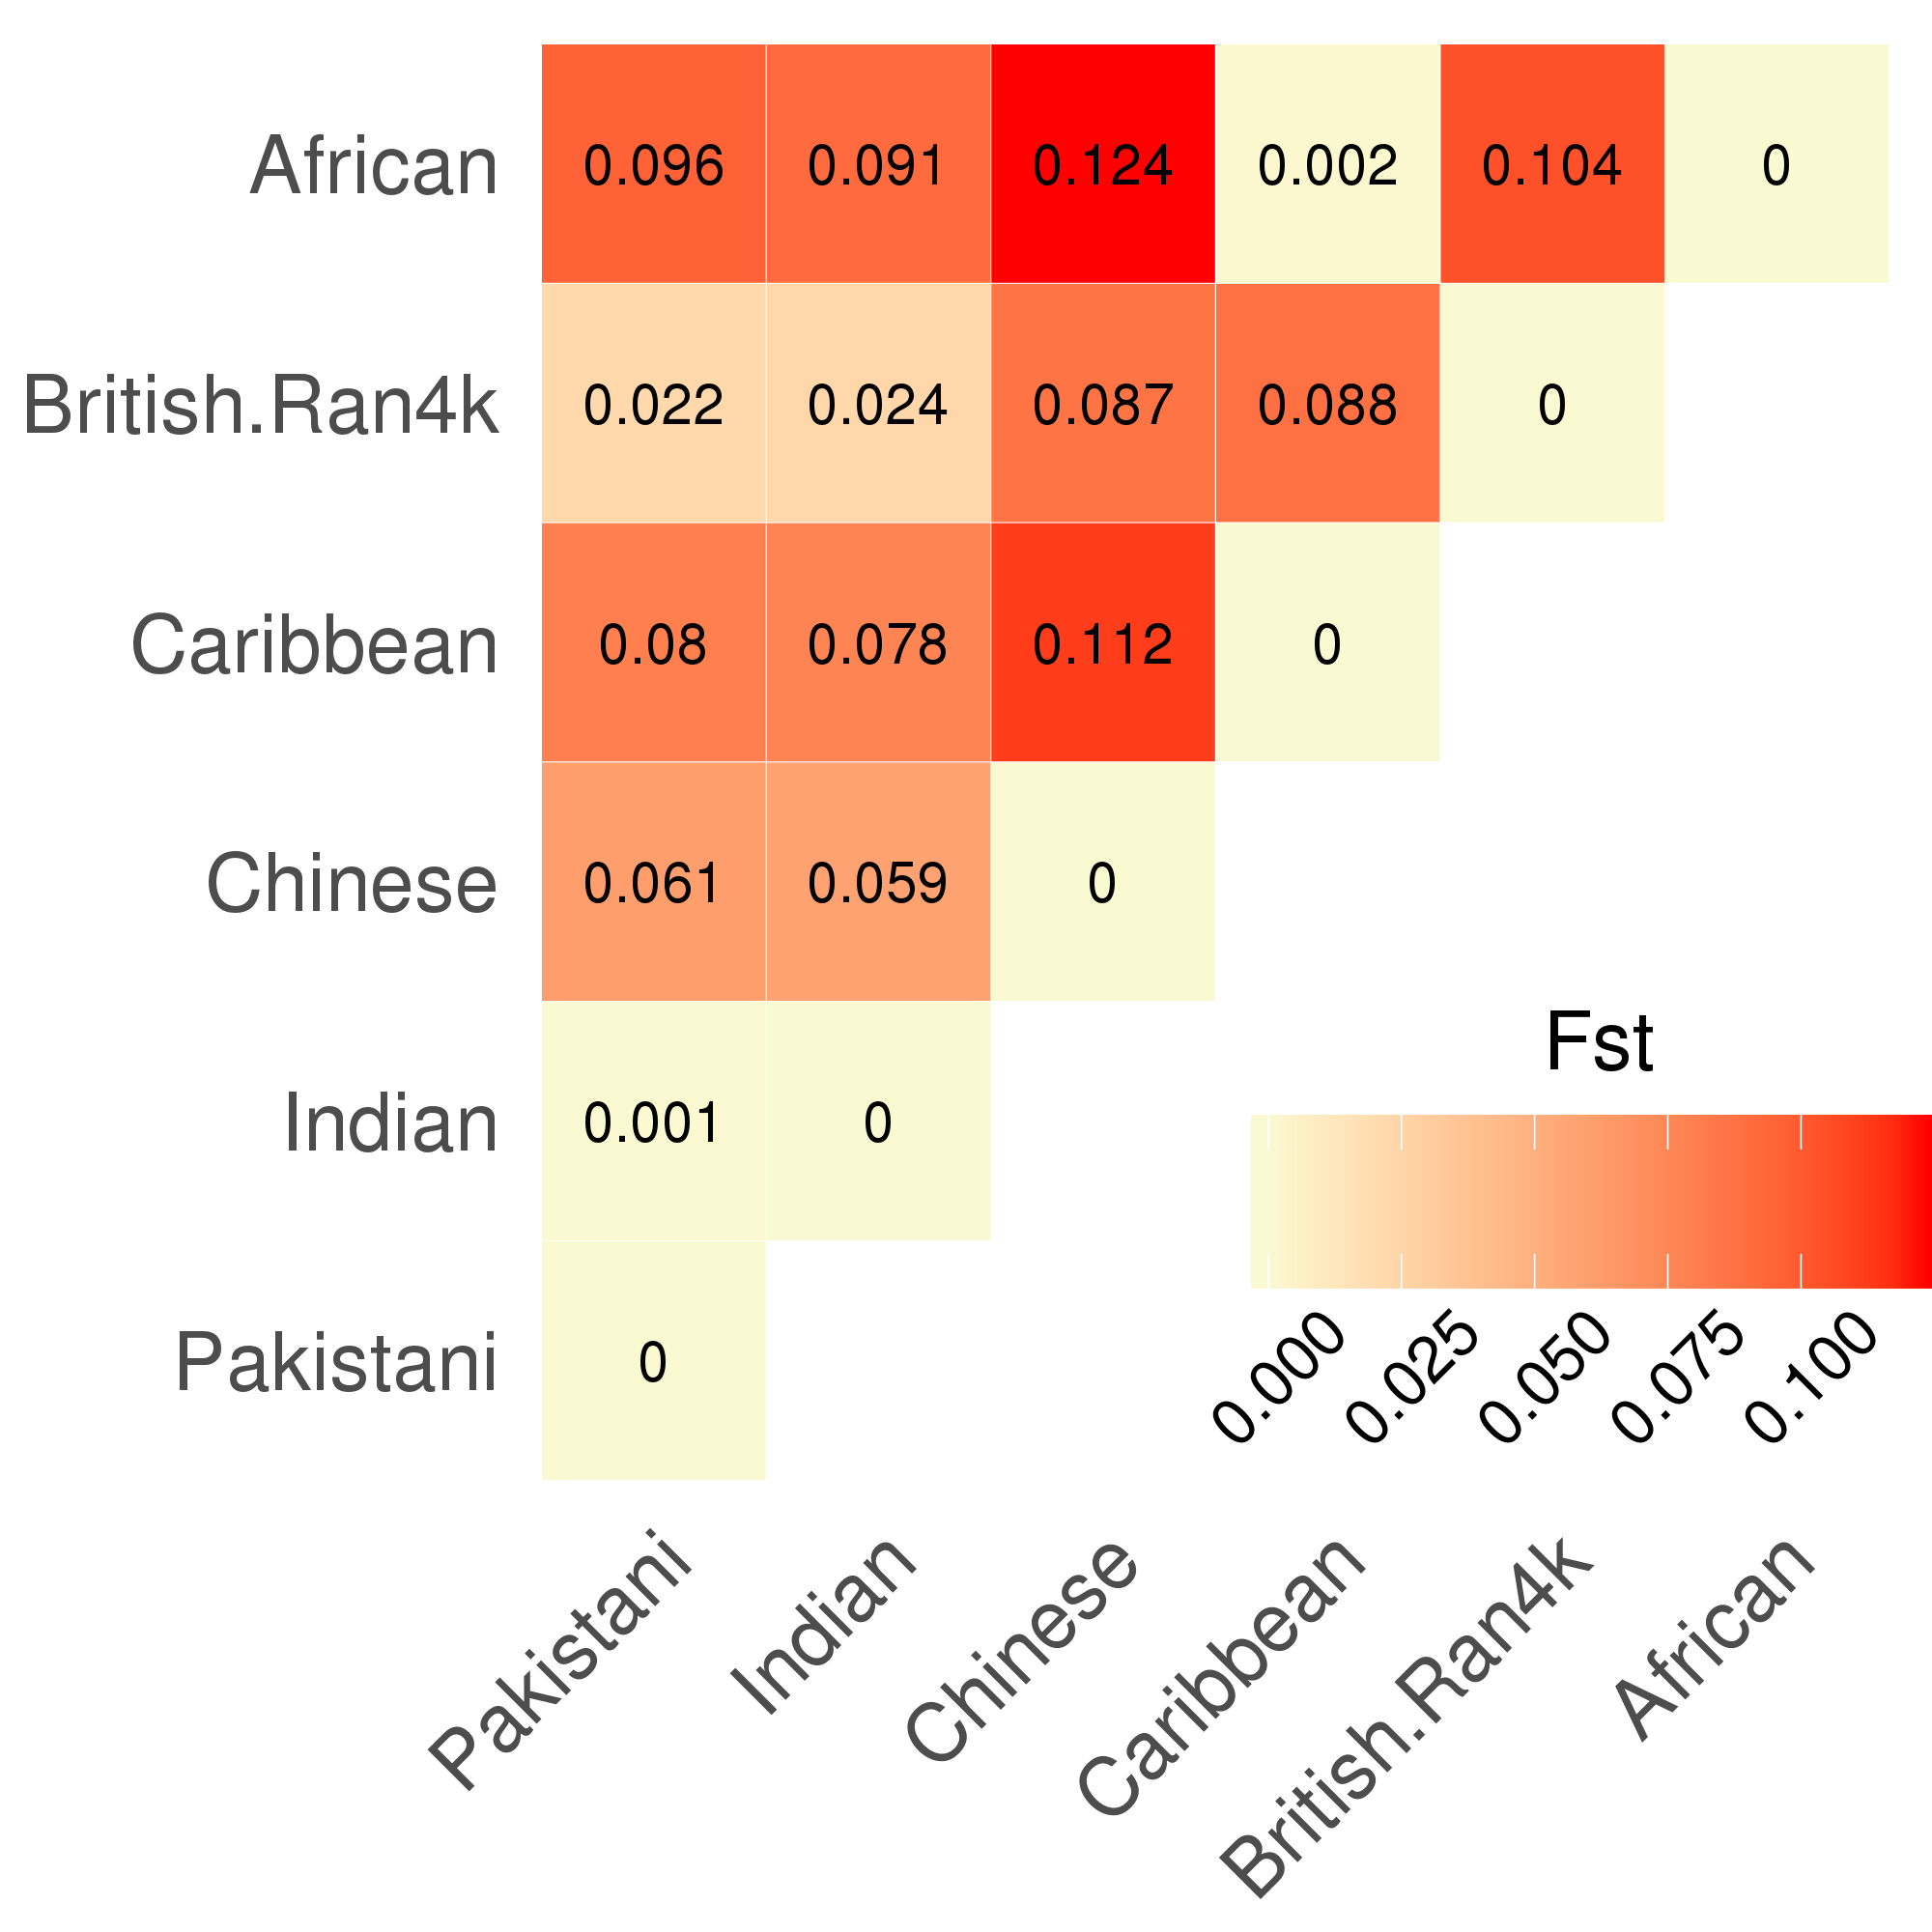
\includegraphics[scale=.5]{Images/Main/InterPath_Main_Figure_Fst_vs2.png}
\caption[TBD]{\textbf{Distribution of pairwise F\textsubscript{ST} across the UKB subgroups}. The heatplot shows pairwise F\textsubscript{ST} values between each of our UKB population subgroups using our genome-wide SNP data. F\textsubscript{ST} values range from .001 to .124, and we observe typical global patterns (eg African and Caribbean being more differentiated versus non-African subgroups, Chinese being more differentiated versus non-Asian subgroups). These global patterns, however, do not match the distribution of total number of significant MAPIT-R pathways observed per-ancestry in Figure \ref{InterPath-Main-Figure-Barplots-KEGG} and Supplementary Figure \ref{InterPath-Supp-Figure-Barplots-REACTOME}.}
\label{InterPath-Main-Figure-Fst}
\end{figure}

To accomplish this, we calculated a pathway-level metric of within-subgroup genetic variation, the mean pairwise proportion of identity-by-state (IBS) per pathway; specifically, for each pathway, we calculated the proportion of IBS between every pair of individuals using the SNPs of the given pathway, and then took the average of this proportion across all pairwise comparisons. Greater levels of genetic variation will correspond with lower levels of IBS, such that proportions of IBS closer to 0 indicate greater levels of genetic variation. Comparing this per-pathway metric of within subgroup genetic variation against each pathway's MAPIT-R $p$-value, we find that there is no significant relationship between the two metrics (Figure \ref{InterPath-Main-Figure-IBS-African} \& Supplementary Figure \ref{InterPath-Supp-Figure-IBS-AllPops}). Shown is the analysis specifically for the African subgroup in the REACTOME database for both height and BMI, but this lack of relationship is observed for almost every combination of phenotype, pathway database, and UKB subgroup. And in directly comparing these analyses between subgroups too, we observe no ancestry-specific patterns aside from general shifts in the average level of mean proportion of pairwise IBS per pathway in line with expected levels of within-ancestry variation (Figure \ref{InterPath-Main-Figure-IBS-AllPopComps-KEGG} \& Supplementary Figure \ref{InterPath-Supp-Figure-IBS-AllPopComps-REACTOME}). 

\begin{figure}[htb]
\centering
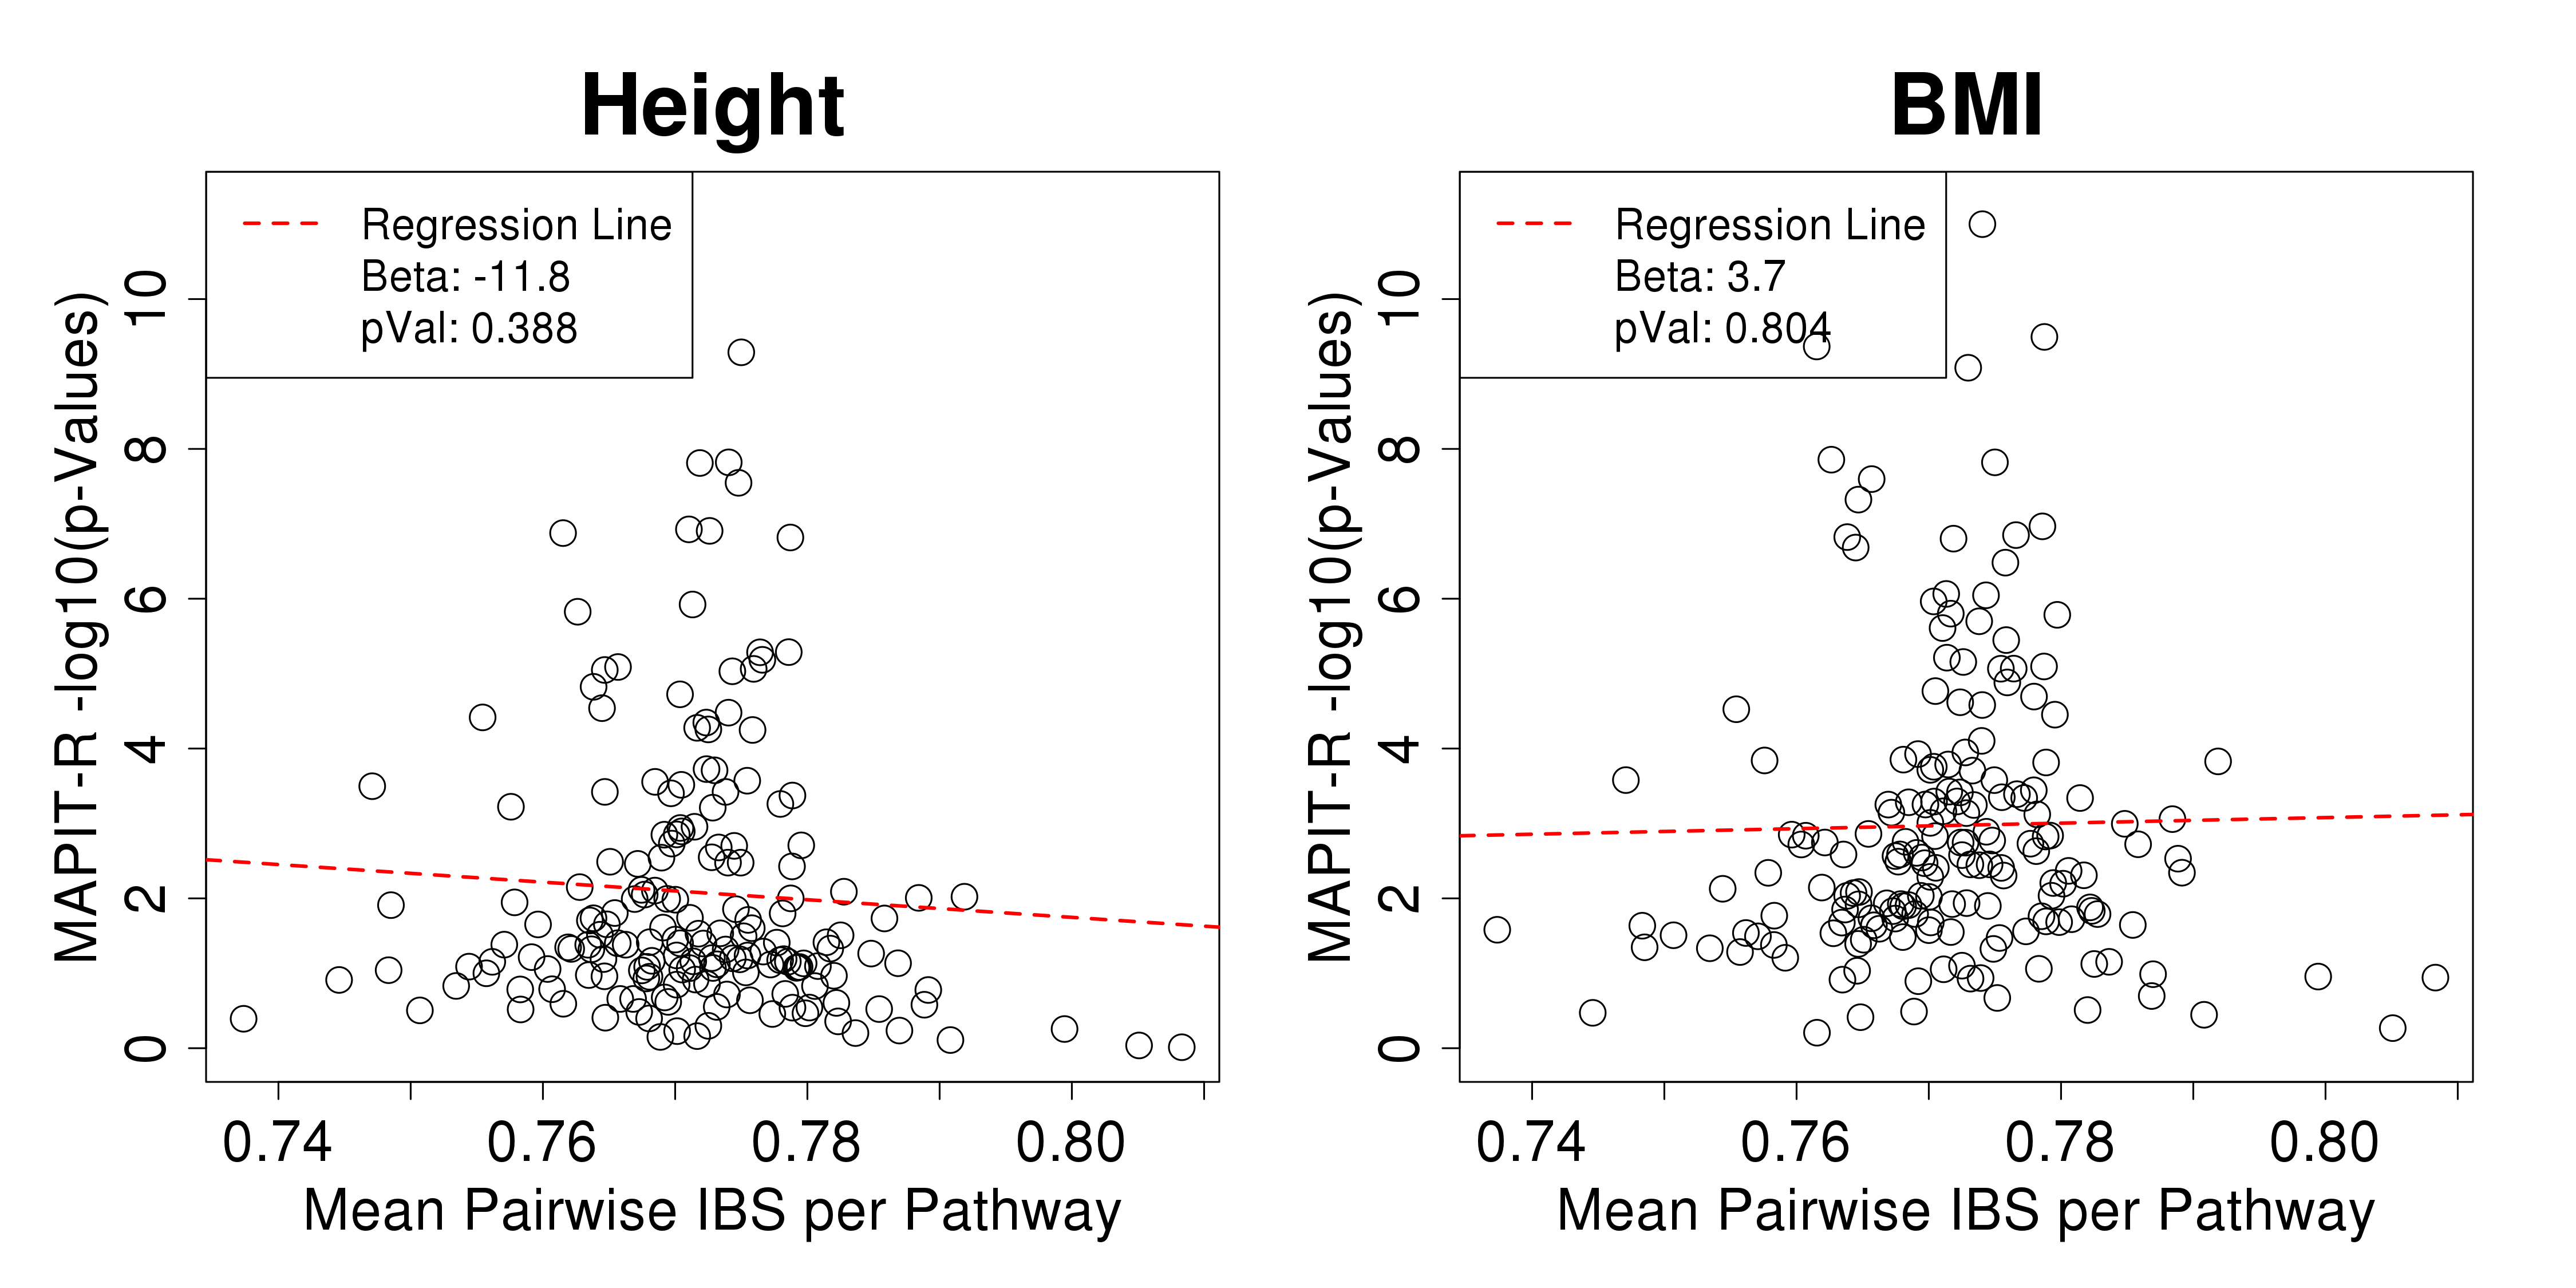
\includegraphics[scale=.35]{Images/Main/InterPath_Main_Figure_IBS_vs3_African.png}
\caption[TBD]{\textbf{Pathway-level genetic diversity versus MAPIT-R results in the African subgroup and KEGG database}. The figure shows the mean pairwise IBS proportions per pathway plotted against each pathway's MAPIT-R $p$-value for the African subgroup KEGG height and BMI analysis. IBS proportions were calculated per pathway by using each pathway's set of SNPs to derive pairwise IBS values between every set of individuals in the subgroup, and then averaging across each of these pairs for a final summary metric. Results for each phenotype, database, and subgroup combination can be found in Supplementary Figure \ref{InterPath-Supp-Figure-IBS-AllPops}. We observe across almost every combination no significant relationship between a pathway's mean pairwise IBS proportion and its MAPIT-R $p$-value.}
\label{InterPath-Main-Figure-IBS-African}
\end{figure}

\begin{figure}[htb]
\centering
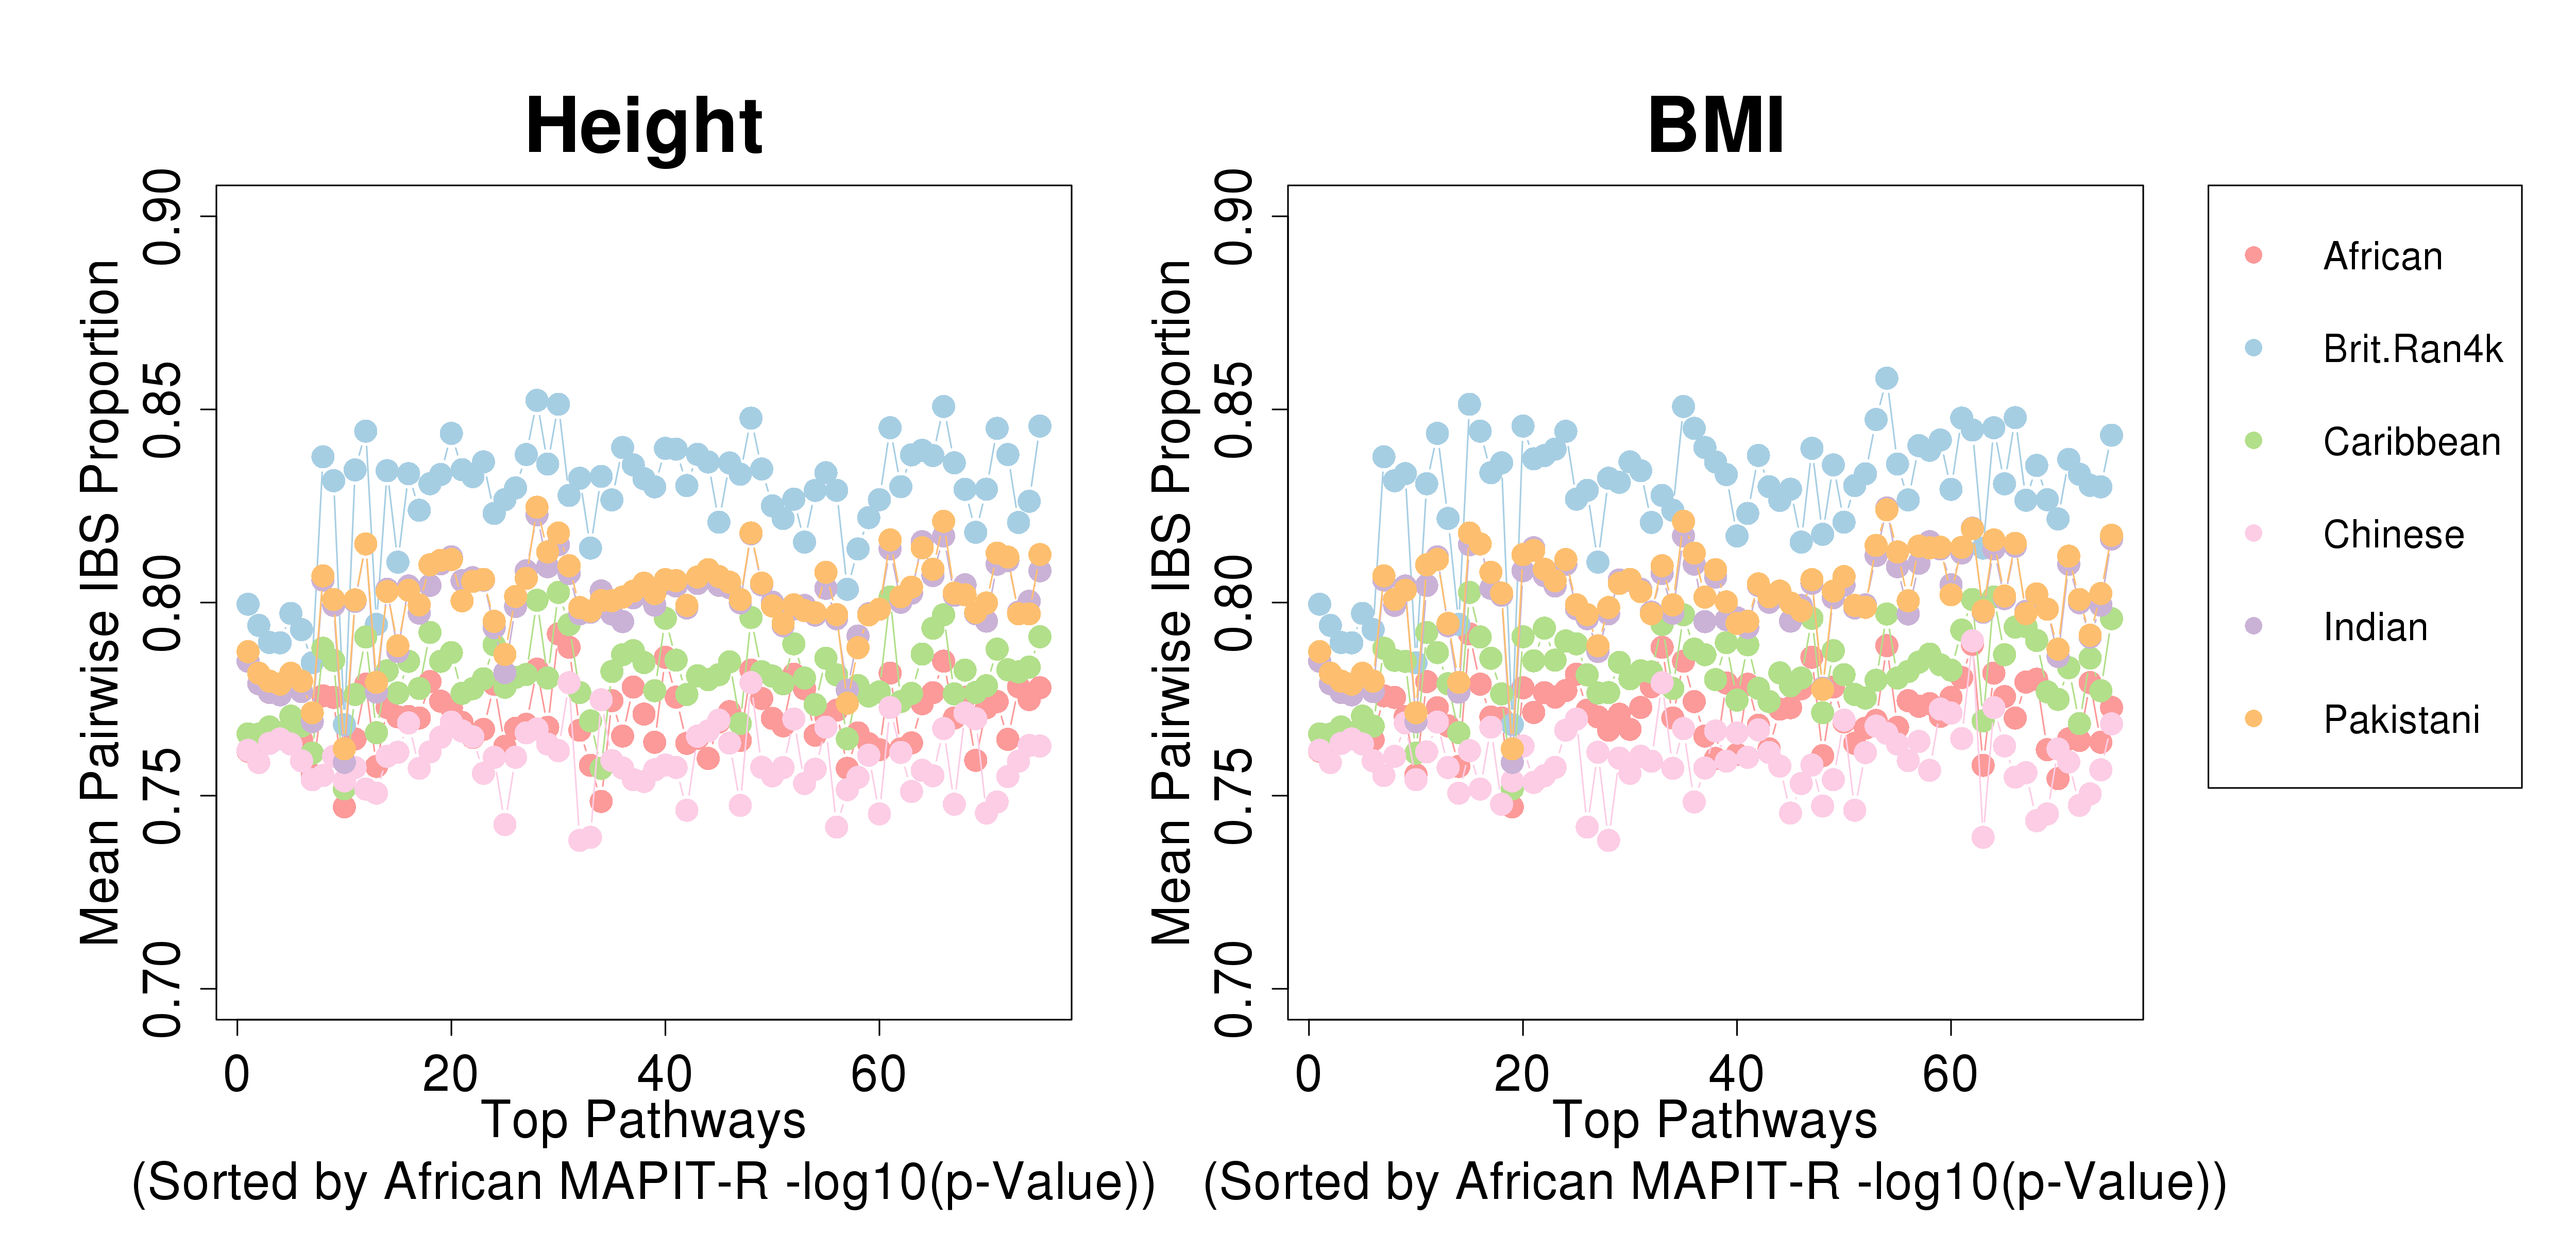
\includegraphics[scale=.35]{Images/Main/InterPath_Main_Figure_IBS_AllPopComps_vs3_KEGG.png}
\caption[TBD]{\textbf{Pathway-level genetic diversity across all UKB subgroups for top African MAPIT-R KEGG pathways}. The figure plots the mean pairwise IBS proportions of each UKB subgroup for the top 75 KEGG pathways (sorted by MAPIT-R African subgroup $p$-value). Mean pairwise IBS proportions appear to follow similar trajectories across each subgroup, shifted mainly by average mean pairwise IBS proportion differences between subgroups. Results for both phenotypes in the REACTOME database can be see in Supplementary Figure \ref{InterPath-Supp-Figure-IBS-AllPopComps-REACTOME}.}
\label{InterPath-Main-Figure-IBS-AllPopComps-KEGG}
\end{figure}

Genome-wide levels of genetic variation do not appear to be a major factor in between-subgrou differences in pathway-level MAPIT-R results, so we then looked at more cryptic\footnote{\textcolor{blue}{MT: we can talk about the use of this word; I've iterated over a few versions, including 'cryptic', 'localized', and 'structured'.}} forms of genetic variation. Specifically, we looked at the PVEs of the within-subgroup principal components we had previously calculated to see if there were any patterns between subgroups that matched the levels of MAPIT-R results we found per subgroup. And indeed, similar to the within-subgroup F\textsubscript{ST} values we saw, we find that subgroup PVE on PC1 matches an order similar to which populations produce the largest numbers of significant pathways (Figure \ref{InterPath-Main-Figure-Eigenvalues}). While this pattern mostly fades by PC3, it may suggest a more complex relationship between within-subgroup genetic variation and MAPIT-R results; possibly, if a pathway had a greater proportion of variants that covered the portions of the genome that were highly loaded on PC1, it might lead to more efficient removal of background population structure. For subgroups that have lower PVEs per PC, reflecting more subtle, less discernible population structure, this may be a less actionable potential benefit.

\begin{figure}[htb]
\centering
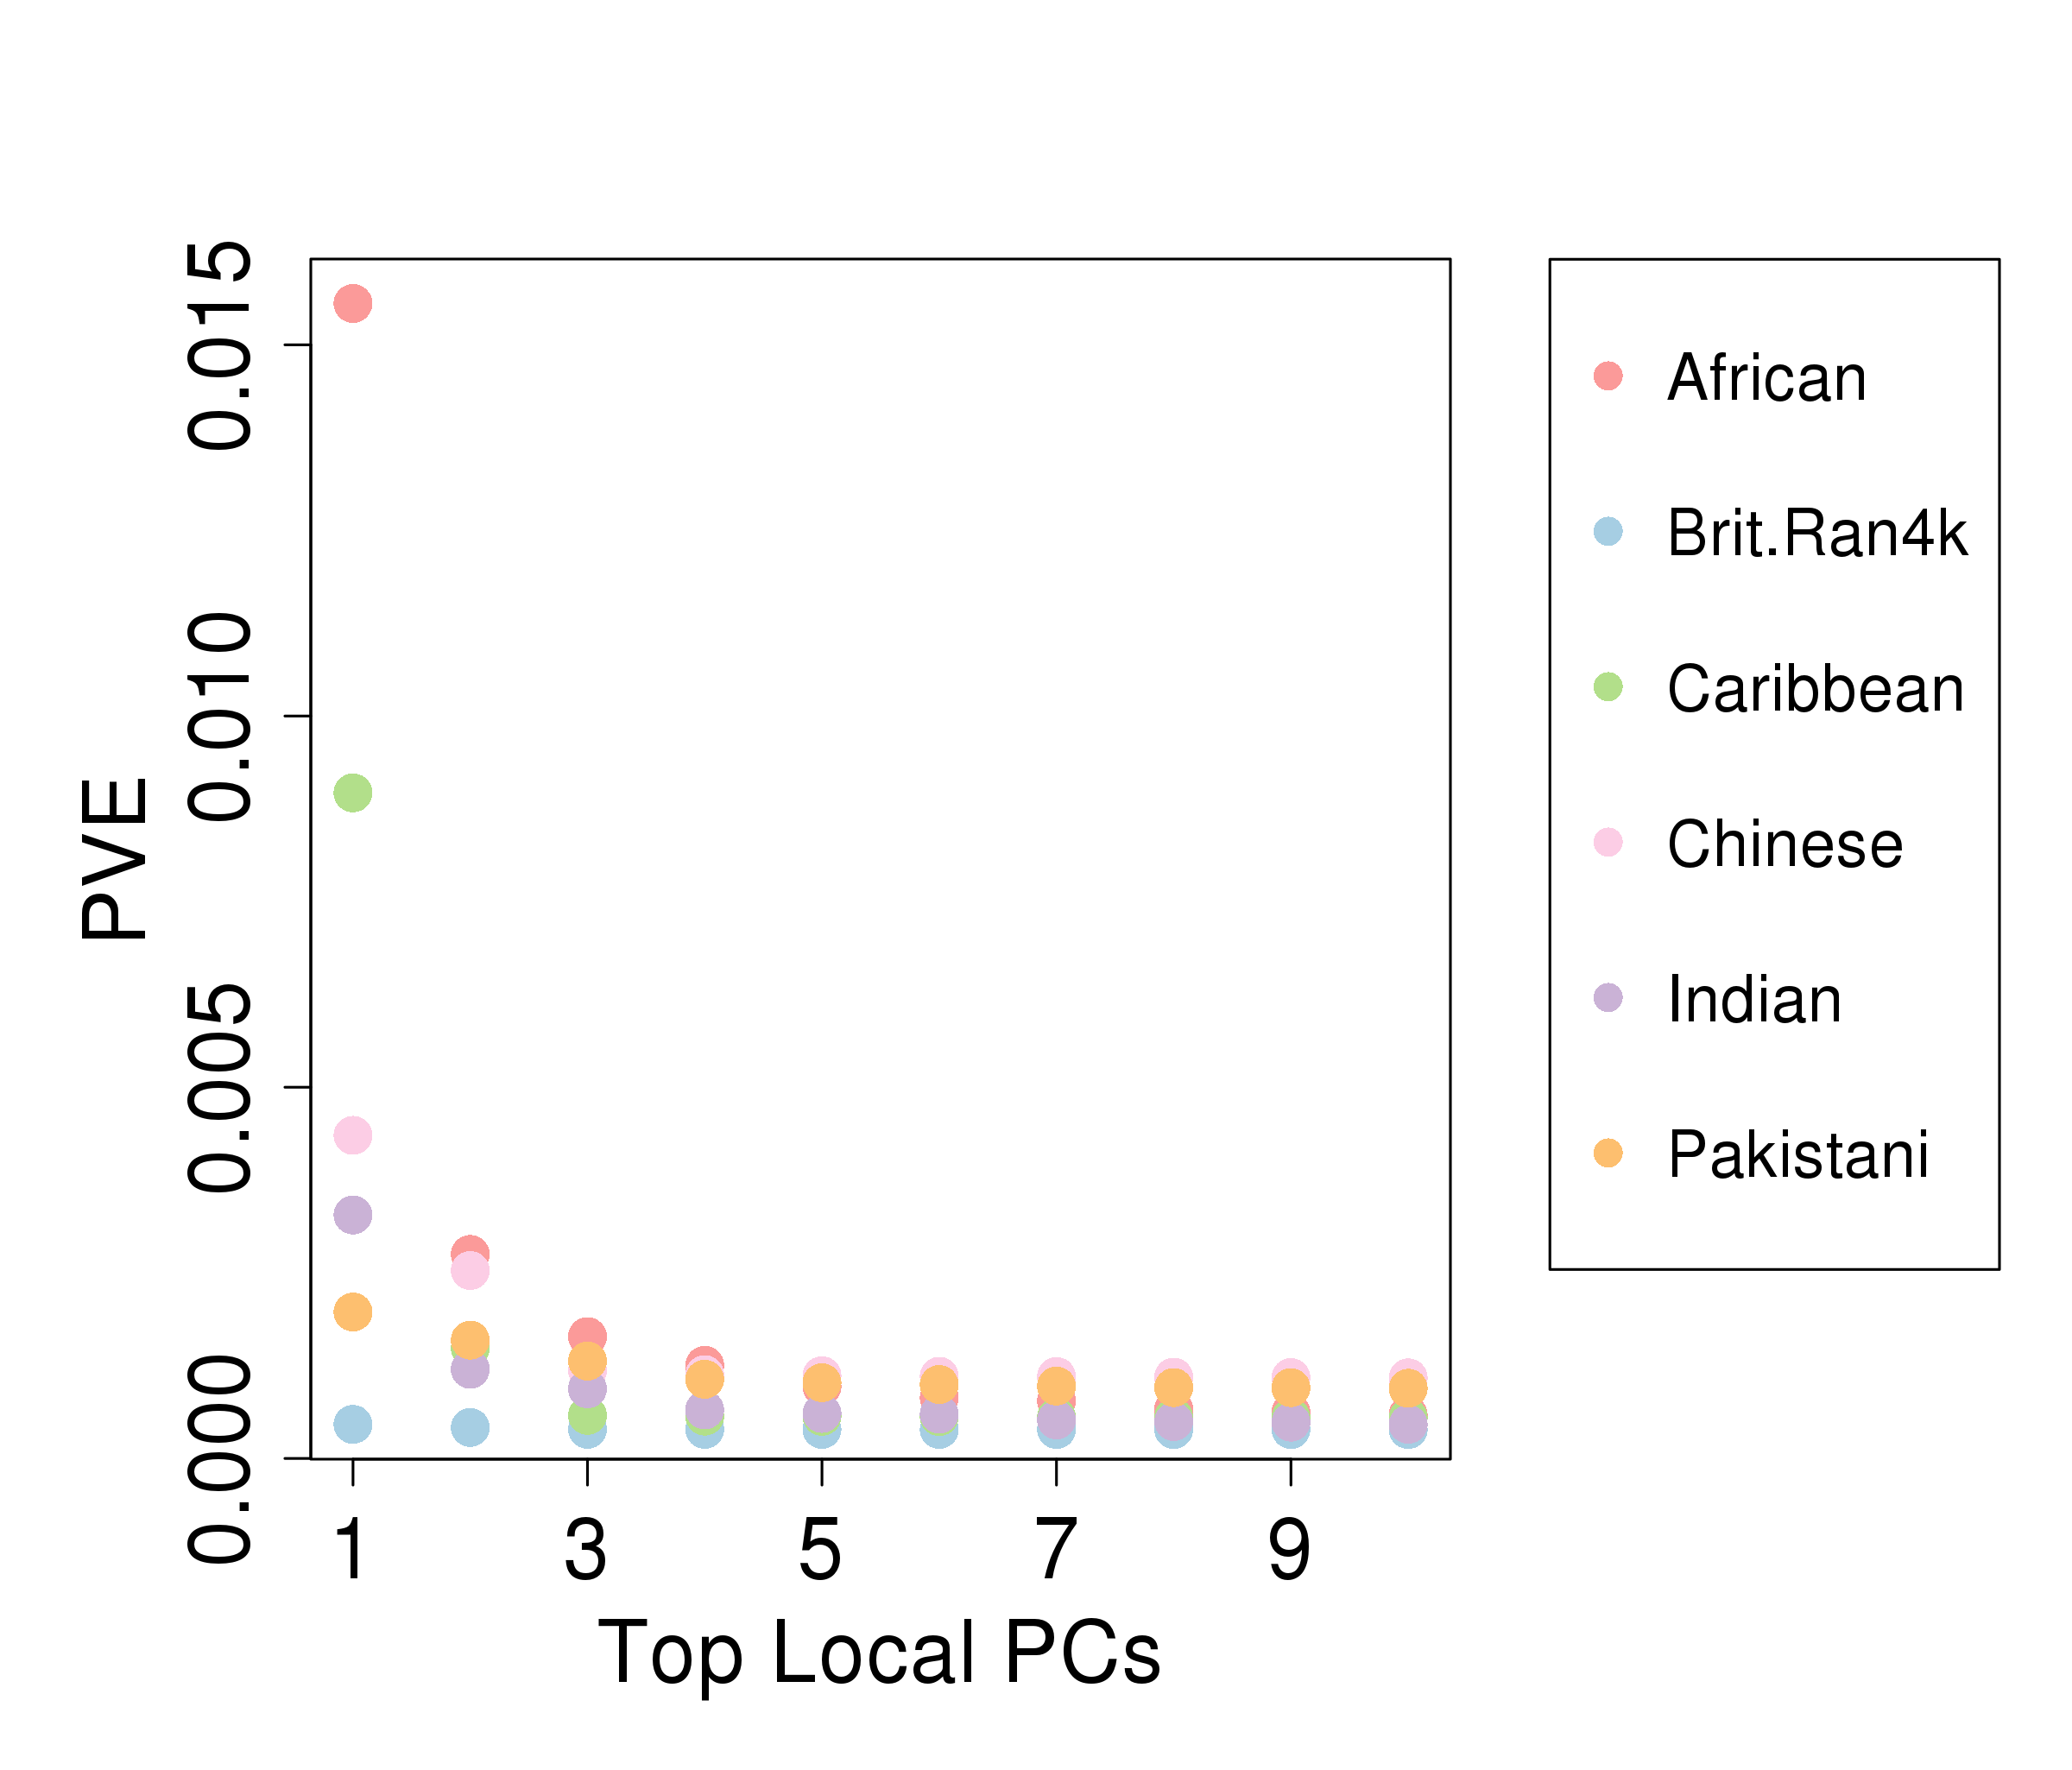
\includegraphics[scale=.45]{Images/Main/InterPath_Main_Figure_Eigenvalues_vs2.png}
\caption[TBD]{\textbf{Distribution of top 10 local principal component PVEs across UKB subgroups}. The plot shows the PVE of each of the top 10 local PCs for each of our UKB population subgroups. Local here continues to refer to calculating PCs within each subgroup separately (versus calculating PCs jointly across all subgroups together). We observe that the distribution of PC1 PVEs among our subgroups appears to strongly correlate with the distribution of total number of genome-wide significant MAPIT-R pathways we identify per subgroup (see Figure \ref{InterPath-Main-Figure-Barplots-KEGG} and  Supplementary Figure \ref{InterPath-Supp-Figure-Barplots-REACTOME}).}
\label{InterPath-Main-Figure-Eigenvalues}
\end{figure}

Therefore, to investigate this possible relationship between subgroup PVE on PC1 and MAPIT-R results, we compared the proportion of SNPs that are strongly loaded on PC1 within a given pathway against that pathway's MAPIT-R $p$-value\footnote{\textcolor{blue}{MT: I'm wondering if we can just say 'strongly loaded' here and define it in the caption of the figure}}. And across both phenotypes in both pathway databases in the African subgroup, we find no significant relationship (Supplementary Figure \ref{InterPath-Supp-Figure-PC1Loading-AllPaths}), nor do we find any significantly positive relationships in any other ancestry subgroup as well. Focusing on pathways with the largest number of SNPs, and therefore potentially the pathways with the largest signals, we do see a marginally significant relationship in the African subgroup using REACTOME pathways (Figure \ref{InterPath-Main-Figure-PC1Loading}; linear regression $p$-value $\approx$ .05), but this result is not replicated in the KEGG pathways. Overall then, it is still unclear if and how within-subgroup genetic variation relates back to the differences between subgroup MAPIT-R results we observe.

\begin{figure}[htb]
\centering
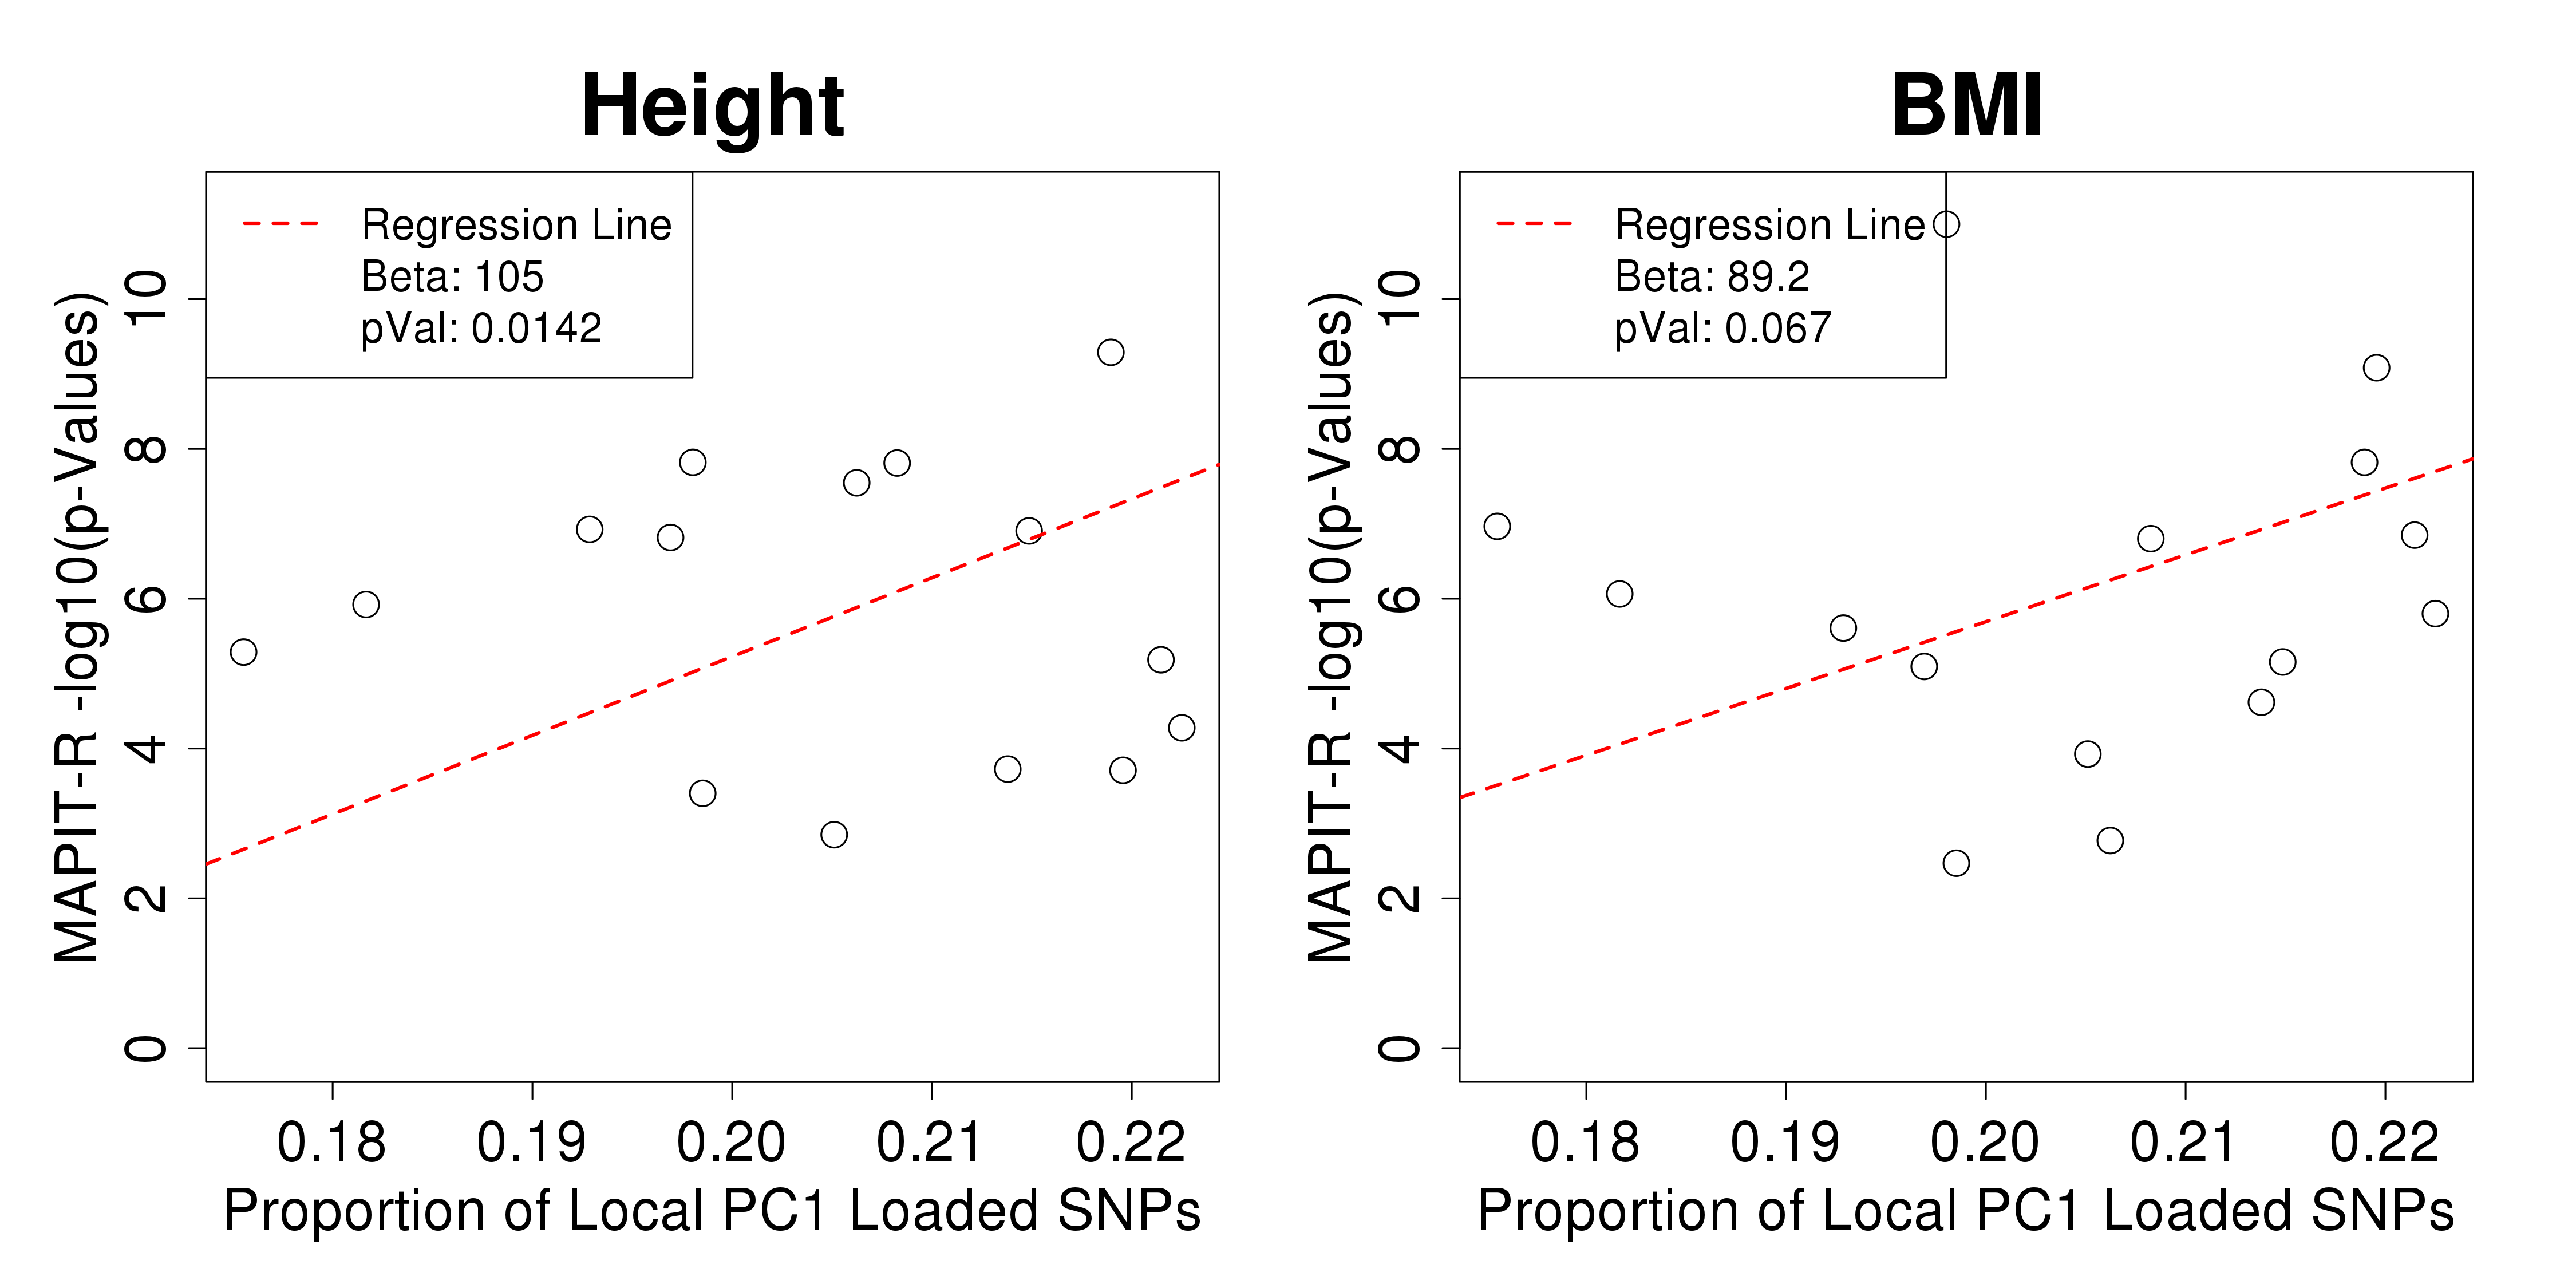
\includegraphics[scale=.35]{Images/Main/InterPath_Main_Figure_PC1Loading_vs1.png}
\caption[TBD]{\textbf{Relationship between MAPIT-R $p$-values and proportions of pathway SNPs loaded on PC1, African subgroup and large pathways}. The figure shows the proportion of SNPs within a given pathway that are strongly loaded on local PC1 plotted against that pathway's MAPIT-R -$\log_{10}$ $p$-value, specifically for the African subgroup and pathways with greater than 1,500 SNPs. `Local' here refers to PCA having been conducted within-subgroup. SNPs are designated as `strongly loaded' on local PC1 if they are within the 10\% tails of the loading SNP score distributions. We observe that there is a marginally significant relationship between MAPIT-R $p$-values and proportion of SNPs that are strongly loaded on PC1, but this is not replicated in the KEGG database.}
\label{InterPath-Main-Figure-PC1Loading}
\end{figure}













\section{Discussion}\label{InterPath-Discussion}

\textcolor{blue}{MT: not updated yet}

Here we present the first exploration of marginal epistasis across multiple human ancestries. Specifically we investigate both single SNP and pathway level marginal epistasis in height and BMI, and present a novel framework for analyzing marginal epistasis in pathways. We find that our African subgroup is particularly well-powered to detect signals of pathway marginal epistasis, with this subgroup containing over 65\% of our 245 total genome-wide hits. We show that across many pathways BMI produces stronger signals of marginal epistasis than height. And lastly, we find evidence that cellular signaling and immune-related pathways may be particularly enriched for marginal epistasis, and the proteasome as a protein complex may be enriched for marginal epistatic interactions as well. 

The fact that we find such an abundance of results in the African UKB subgroup is not necessarily surprising. The notion that African populations may be particularly insightful for complex trait genetics is not novel \citep{Rotimi2017,Choudhury2018,Martin2018,Bentley2020}, with efforts delineating the genetic architecture of skin pigmentation \citep{Martin2017b,Crawford2017b} and the evolutionary histories of FOXP2 and other loci \citep{Atkinson2018,Sugden2018} being some recent examples. The question of what aspects of the greater genetic diversity observed in African populations is driving the results found here is still an area of future work. As we have found initially, it is unlikely that our results are due to broadscale differences between populations in pathway-level genetic variation alone. Instead, what we may be observing is differences in observable population structure leading to variation in the ability to correct for background noise; the higher PC1 PVE observed in the African population may be evidence that being able to remove a greater amount of structure from the data leads to more exposure of the underlying genetic signal. Future work based on these results should include further exploration of this connection between patterns of genetic variation and power to detect epistatic signals in the African subgroup.  

While the results presented here are encouraging on multiple levels, there are some limitations to the current analyses. One major future direction for work is the need for scaling these types of marginal epistasis methods. Similar to MAPIT, MAPIT-R currently does not scale well to the full sizes of current biobanks; in its current form MAPIT-R may begin to encounter burdensome computational times beyond 20,000 individuals. One potential avenue to overcome these issues is to incorporate the use of summary statistics for the analysis of marginal epistasis; moving from direct genotypes to GWA study summary statistics has proven useful in both speeding up computational time as well as increasing power in multiple other GWA contexts \citep{Shi2016,Johnson2018,Ray2018,Cheng2019,Turchin2019,Urbut2019}. Another limitation of MAPIT-R is that, as part of the marginal epistasis framework, it identifies whether a pathway contains any epistatic interactions with the rest of the genome. As shown here this has the advantage of accumulating signal over multiple variants, but it produces an ambiguous situation in terms of what regions of the genome to analyze \textit{a posteriori}. Extending or linking MAPIT-R with a framework that explicitly follows up marginal epistasis signals with locus-focused methods such as fine-mapping \citep{Kichaev2014,Chen2015,Benner2016} or co-localization \citep{Hormozdiari2016,Zhu2016,Wen2017,Giambartolomei2018,Wallace2020} may further expand the power of the marginal epistasis approach.  

\section{Methods}\label{InterPath-Online-Methods}

\subsection{UK BioBank Data}

\subsubsection{Population subgroups}

To create the UKB population subgroups used in this study, we first extracted and grouped individuals by the self-identified ancestries of `African', `British', `Caribbean', `Chinese', `Indian', and `Pakistani'. British random subgroups of 4,000 and 10,000 individuals, both the original sets and the additional four rounds of replications, were constructed by randomly choosing initial sets of non-overlapping 4,000 and 10,000 individuals. Standard quality control (QC) procedures were then employed on each population subgroup (see Supplementary Note for details) on both the variant and individual levels, pre-PCA. Local PCA was then conducted to confirm ancestry groupings and remove outliers, and a last round of QC was conducted post-PCA as well. Note that the genetic data used in these analyses were the directly genotyped variant sets  from the UKB after running imputation on the University of Michigan Imputation Server \citep{Das2016}; most of the analyses in this manuscript utilize genetic relatedness matrices (GRMs), and GRMs require zero genotype missingness. To minimize the loss of SNPs while meeting this threshold we chose to impute missing genotypes while still focusing on just the original set of genotyped variants. For metrics and PCA plots of the final, post-QC set of UKB individuals, see Supplementary Figure \ref{InterPath-Supp-Figure-UKB-subgroups-PCAPlot} and Supplementary Table \ref{InterPath-Supp-Table-UKBPopStats}. 

\subsubsection{Phenotypes}

For the analyses presented in this study we focused on the complex traits of height and BMI. Each phenotype was adjusted for age, gender, and assessment center. Following previous pipelines \citep{Wood2014,Locke2015}, each dataset was first divided into males and females. Age was then regressed out within each sex, and the resulting residuals were inverse normalized. These normalized values were then combined back together between sexes and, lastly, assessment center designations were regressed out. 

\subsection{PLINK Analyses}

PLINK pairwise epistasis analyses were conducted using PLINK v1.90b4 \citep{Purcell2007}, the `\texttt{-{}-epistasis}' command, and phenotypes that had top 10 local PCs regressed out; PCs were regressed out directly from the phenotypes due to the `\texttt{-{}-epistasis}' function having no explicit form to incorporate covariates. Default values for the `\texttt{-{}-epi1}' and `\texttt{-{}-epi2}' options (0.0001 and 0.01, respectively) were kept.   

\subsection{MAPIT Analyses}

MAPIT analyses were conducted using the MAPIT software downloaded from \url{https://github.com/lorinanthony/MAPIT}. MAPIT was run using the phenotypes as previously described and top 10 local PCs as covariates. Specifically, we used the `\texttt{MAPIT\_Davies\_Approx}' function due to its computational speed up and because our datasets had large enough sample sizes to properly employ the approximate form.  






\subsection{MAPIT-R Model}

\textcolor{red}{Reminder: we regress the additive genotypes out of the phenotype now instead of including that information in the m-projection matrix}

We describe the framework for ``\underline{Inter}actions in \underline{Path}way'' (MAPIT-R) analysis in detail here. The key goal of this method is to identify crosstalk between signaling pathways in GWA studies, without having to explicitly model all possible higher-order interactions. In general, consider a pathway which is defined by a set of SNPs found within the regulatory regions of genes in that pathway. We will denote these variants with the set of indices $\mathcal{R} = (r_1,\ldots,r_p)$. Begin by considering the following partitioned linear regression model,
\begin{equation}\label{LM}
\by = \mu\bm{1}+\sum_{r\in \mathcal{R}}\bx_r\beta_{r}+\sum_{s\not\in \mathcal{R}}\bx_s\beta_{s}+\bvarepsilon, \quad \bvarepsilon\sim \mathcal{N}(\mathbf{0}, \tau^2\bI),
\end{equation}
where $\by$ is an $n$-dimensional vector of quantitative phenotypes for $n$ individuals; $\mu$ is an intercept term with an $n$-dimensional vector of ones; $\bx_r$ and $\bx_s$ are $n$-dimensional genotype vectors for variants that lie within and outside the regulatory region $\mathcal{R}$, respectively; $\beta_r$ and $\beta_s$ are the corresponding additive effect sizes; $\bvarepsilon$ is an $n$-vector of residual errors; $\tau^2$ is the residual error variance; $\bI$ denotes the identity matrix; and $\mathcal{N}(\bullet,\bullet)$ denotes a multivariate normal distribution. Here, we also assume that the genotypic vectors have been centered and standardized to have mean 0 and standard deviation 1.

Because we consider scenarios where there are more variants than samples, we need to specify additional modeling assumptions in Equation \eq{LM} to make the rest of the model identifiable. In particular, we recall previous approaches and assume that the individual effect sizes follow univariate normal distributions, or $\beta_r \sim \mathcal{N}(0, \omega^2/p)$ and $\beta_s \sim \mathcal{N}(0, \sigma^2/(l-p))$, where $l$ is the number of total number of all SNPs \citep{Crawford2017a}. With the assumption of normally distributed effect sizes, the model defined in Equation \eq{LM} is equivalent to a variance component model where $\bg\sim \mathcal{N}(\bm{0}, \omega^2\bK)$ with $\bK=\bX_{\mathcal{R}}\bX_{\mathcal{R}}^{\T}/p$ being the genetic relatedness matrix computed using genotypes from all variants within the signaling pathway of interest; and $\wt\bg\sim \mathcal{N}(\bm{0}, \nu^2\wt\bK)$ with $\wt\bK=\bX_{-\mathcal{R}}\bX_{-\mathcal{R}}^{\T}/(l-p)$ representing a relatedness matrix computed using all other variants. Note that $\bg$ may be interpreted as a pathway's additive effect, while $\wt\bg$ denotes its polygenic background. 

To complete the specification of the MAPIT-R methodology, we lastly assume an additional random effect $\bu$ which models the summation of all pairwise interaction effects between a given signaling pathway variant and all other pathways. In this work, we limit ourselves to the case of finding second order crosstalk relationships between pathways --- although, extensions to higher-order interactions is straightforward \citep{Crawford2017a}. Altogether, this results in the following linear mixed model
\begin{equation}
\by = \mu\bm{1}+ \bg +\wt\bg+\bu+\bvarepsilon,\\ 
\bg\sim \mathcal{N}(\bm{0}, \omega^2\bK), \quad \wt\bg\sim \mathcal{N}(\bm{0},
\nu^2\wt\bK),\\ 
\bu\sim\mathcal{N}(\bm{0},\sigma^2\bQ), \quad \bvarepsilon\sim \mathcal{N}(\mathbf{0}, \tau^2\bI).\label{LMM}
\end{equation}
Here, the $\bQ = \bK\circ\wt\bK$ is represents a second-order interaction relationship matrix, and is obtained by using the Hadamard product (i.e.~the squaring of each element) between the pathway specific relatedness matrix and its corresponding polygenic background. Note that the formulation of MAPIT-R in Equation \eq{LMM} can easily be extended to accommodate other fixed effects (e.g.~age, sex, or genotype principal components), as well as other random effects terms that can be used to account for sample non-independence due to other genetic or common environmental factors.

%Note that we make the assumption that each $\bg_k^{(l)}\sim \mbox{MVN}(\bm{0}, \sigma_{l}^2\bK^l_k)$, where the baseline covariance matrix $\bK_k=\bX_{-\mathcal{R}}\bX_{-\mathcal{R}}^{\T}/p_k$ is the conventional genetic relatedness matrix computed using genotypes from all $p_k$ variants outside of the region $\mathcal{R}$. Here, we use the power factor $l$ to denote the order of interaction (epistatic) effects that are accounted for within the model. For example, when $l=2$, $\mathbf{K}_k^2 = \mathbf{K}_k\circ\mathbf{K}_k$ represents a pairwise interaction relationship matrix, and is obtained by using the Hadamard product (i.e.~the squaring of each element) of the linear kernel matrix with itself \citep{Henderson:1985aa,Ronnegard:2008aa,Jiang:2015aa}. In this case, $\mathbf{K}_k^2$ denotes the marginal second order epistatic effect of the $k$\textsuperscript{th} functional marker under the polygenic background of all other markers. It is important to note that each $\bK_k^{l}$ changes with every new gene, protein, or pathway $k$ that is considered.

\subsection{Hypothesis Testing for Interaction Effects}

Our goal is to identify signaling pathways that have significant non-zero interaction effects on a given phenotype. To do so, we examine each $r$-th pathway of interest in turn, and test the null hypothesis in Equation \eqref{LMM} that $\text{H}_0: \sigma^2=0$. The variance component $\sigma^2$ effectively captures the total interaction effects between the $r$-th pathway and all other pathways. We refer to this as the marginal interaction effect for the $r$-th pathway. To do so, we make use of the MQS method for parameter estimation and hypothesis testing \citep{Zhou2017}. Briefly, MQS is based on the computationally efficient method of moments and produces estimates that are mathematically identical to the Haseman-Elston (HE) cross-product regression \citep{Haseman1972}. To estimate the variance components with MQS, we first multiply Equation \eq{LMM} by a projection (hat) matrix onto the null space of the intercept term $\mu$, where $\bH=\bI-\bm{1}(\bm{1}^{\T}\bm{1})^{-1}\bm{1}^{\T}$. After this projection procedure, we obtain a simplified linear mixed model 
\begin{equation}
\by^*_r = \bg^*_r +\wt\bg^*_r+\bu^*_r+\bvarepsilon^*_r\\ 
\bg_r\sim \mathcal{N}(\bm{0}, \omega^2\bK^*_r), \quad \wt\bg_r\sim \mathcal{N}(\bm{0}, \nu^2\wt\bK^*_r),\\ \bu_r\sim\mathcal{N}(\bm{0},\sigma^2\bQ^*_r), \quad \bvarepsilon_r\sim \mathcal{N}(\mathbf{0}, \tau^2\bH) \label{LMM2}
\end{equation}
where $\by^*_r=\bH\by$; $\bg^*_r = \bH\bg_r$; $\bK^*_r = \bH\bK_r\bH$; $\wt\bg_r^* = \bH\wt\bg_r$; $\wt\bK_r^* = \bH\wt\bK_r\bH$; $\bu^*_r = \bH\bu_r$; $\bQ^*_r = \bH\bQ_r\bH$; and $\bvarepsilon_r^* = \bH_r\bvarepsilon$, respectively. Then for each pathway considered, the MQS estimate for the marginal interaction effect is computed as
\begin{equation}
\wh\sigma^2 = \by^{*\T}_r\bA_r\by
\end{equation}
where $\bA_{r} = (\bS_r^{-1})_{31}\bK_r^*+(\bS_r^{-1})_{32}\wt\bK_r^*+(\bS_r^{-1})_{33}\bQ^*_r+(\bS_r^{-1})_{34}\bH$ with elements $(\bS_r)_{jk} = \tr(\bSigma_{rj} \bSigma_{rk})$ for the covariances matrices subscripted as $[\bSigma_{r1}; \bSigma_{r2}; \bSigma_{r3}; \bSigma_{r4}]  = [\bK^*_r; \wt\bK^*_r; \bQ^*_r; \bH]$. Here, $\tr(\bullet)$ is used to denote the matrix trace function. It has been shown that, under MQS, a given marginal variance component estimate $\wh\sigma^2$ follows a mixture of chi-square distributions under the null hypothesis \citep{Crawford2017a}. Namely, $\wh\sigma^2 \sim \sum_{i=1}^{n}\lambda_{i}\chi^2_{1,i}$, where $\chi^2_{1}$ are chi-square random variables with one degree of freedom and $(\lambda_{1},\ldots,\lambda_{n})$ are the eigenvalues of the matrix 
\begin{equation*}
\left(\wh\omega^2_{0}\bK^*_r+\wh\nu^2_{0}\wt\bK^*_r+\wh\tau^2_{0}\bH\right)^{1/2} \bA_{r}\left(\wh\omega^2_{0}\bK^*_r+\wh\nu^2_{0}\wt\bK^*_r+\wh\tau^2_{0}\bH\right)^{1/2}
\end{equation*}
with $(\wh\omega^2_{0},\wh\nu^2_{0},\wh\tau^2_{0})$ being the MQS estimates of $(\omega^2,\nu^2,\tau^2)$ under the null hypothesis. Several approximation and exact methods have been suggested to obtain p-values under the distribution of $\wh\sigma^2$. One frequented choice is Davies exact method \citep{Davies1980,Wu2011}. 

%\subsection*{Hypothesis Testing for Overall Associations}

%FORCE also provides an option for summarizing overall marker enrichment. Here, we assume that we have already computed the $q$ marginal effect p-values for genetic marker $k$, denoted as $\wh\bp_k = (\wh p_{k1},\ldots,\wh p_{kq})$. Let $\wh\balpha_k^* = F^{-1}(\wh\bp_k)$ be the transformed test statistic where $F^{-1}$ is the inverse of the cumulative distribution function (CDF) of the standard chi-square $\chi^2_1$. We follow previous works and define the sum of the correlated chi-square variables for a given functional genomic marker as \citep{Nakka:2016aa}
%\begin{equation}
%\bar{\alpha}_k^* = \sum_{l=1}^{q}\wh\alpha_{k,l}^*.\label{Comp}
%\end{equation}
%(NOTE: Follow the rest of the language from methods in PEGASUS here).


\subsection{MAPIT-R Analyses}


\section{URLs}\label{InterPath-URLs}

MAPIT: \url{https://github.com/lorinanthony/MAPIT}

MAPIT-R: \url{https://github.com/mturchin20/MAPIT-R}

\section{Acknowledgments}\label{InterPath-Acknowledgments}

This material is based upon work supported by the National Science Foundation under Grant No. DMS-1439786 while G.D. was in residence at the Institute for Computational and Experimental Research in Mathematics in Providence, RI, during the model and dimension reduction in uncertain and dynamic systems program.

\section{Author Contributions}\label{InterPath-Author-Contributions}

\section{Competing Interests}\label{InterPath-Competing-Interests}

\section{Supplementary Note}\label{Supplementary-Note}

\subsection{Population Subgroup Quality Control}

We conducted standard quality control (QC) procedures on each of these population subgroups. Note that we focused our analyzes on the genotyped chip data throughout the project. First we conducted SNP-level QC by dropping variants that did not meet the following criteria:  minor allele frequency (MAF) $>$ .01, genotype missingness $<$ 5\%, and Hardy-Weinberg equilibrium test $p$-value $>$ $1\times10^{-6}$. We then conducted individual-level QC via the following steps. Individuals were removed if they did not have genotype missingness $>$ 5\%. Individuals were also removed if they were a 3\textsuperscript{rd} degree relative or more to someone else in the dataset; specifically the KING relatedness values provided with the UKB data were used to identify related individuals, and one individual from every pair of 3\textsuperscript{rd} degree or more relatives was removed. Individuals were also dropped if they were tagged by any of the following three flags from the UKB data: `het.missing.outliers', `putative.sex.chromosome.aneuploidy', and `excess.relatives'. Lastly, individuals were removed if they were determined to be PCA outliers; this was conducted by running FlashPCA (version 2.1) \citep{Abraham2017} in R on each population subgroup separately and identifying individuals that had PC values greater than 7 standard deviations away from the mean for any of the top 6 PCs. We refer to conducting PCA on each subgroup separately as 'local PCA' to help distinguish from the alternative setup of conducting PCA on the entire dataset jointly, which would be referred to as 'global PCA'. 

After this first round of QC procedures, we then proceeded to impute our current population subgroups. Since most of the analyses in this project utilized genetic relatedness matrices (GRMs), and variants need to have no missing data for these GRMs, we used imputation primarily to maximize the number of genotyped SNPs that would not be dropped by this stringent threshold (as opposed to using imputation to increase the number of SNPs we were analyzing). To conduct this imputation, we uploaded our population subgroups to the University of Michigan Imputation Server \citep{Das2016} and used the following options: Minimac3 for the imputation software, 1000G phase 3 v5 for the reference panel, and Eagle v2.3 for the phasing software. Completed imputed files were then downloaded from the Imputation Server afterwards and treated to further QC steps: imputed variants were intersected back to the original set of genotyped chip variants, variants with imputation quality scores $<$ .3 were removed, and variants that had genotype missingness rates $>$ 0\% were also removed. These steps represent the last of our QC and imputation procedures, and information on the final forms of our UKB population subgroups can be found in Supplementary Table (table).

\clearpage


\section{Supplementary Figures}\label{Supplementary-Figures}

%\renewcommand{\thefigure}{Supplementary \arabic{figure}}
%\renewcommand{\thetable}{Supplementary \arabic{table}}
\renewcommand{\figurename}{Supplementary Figure}
\renewcommand{\tablename}{Supplementary Table}
\setcounter{figure}{0}
\setcounter{table}{0}

\begin{figure}[htbp]
\centering
\hspace*{-1cm}
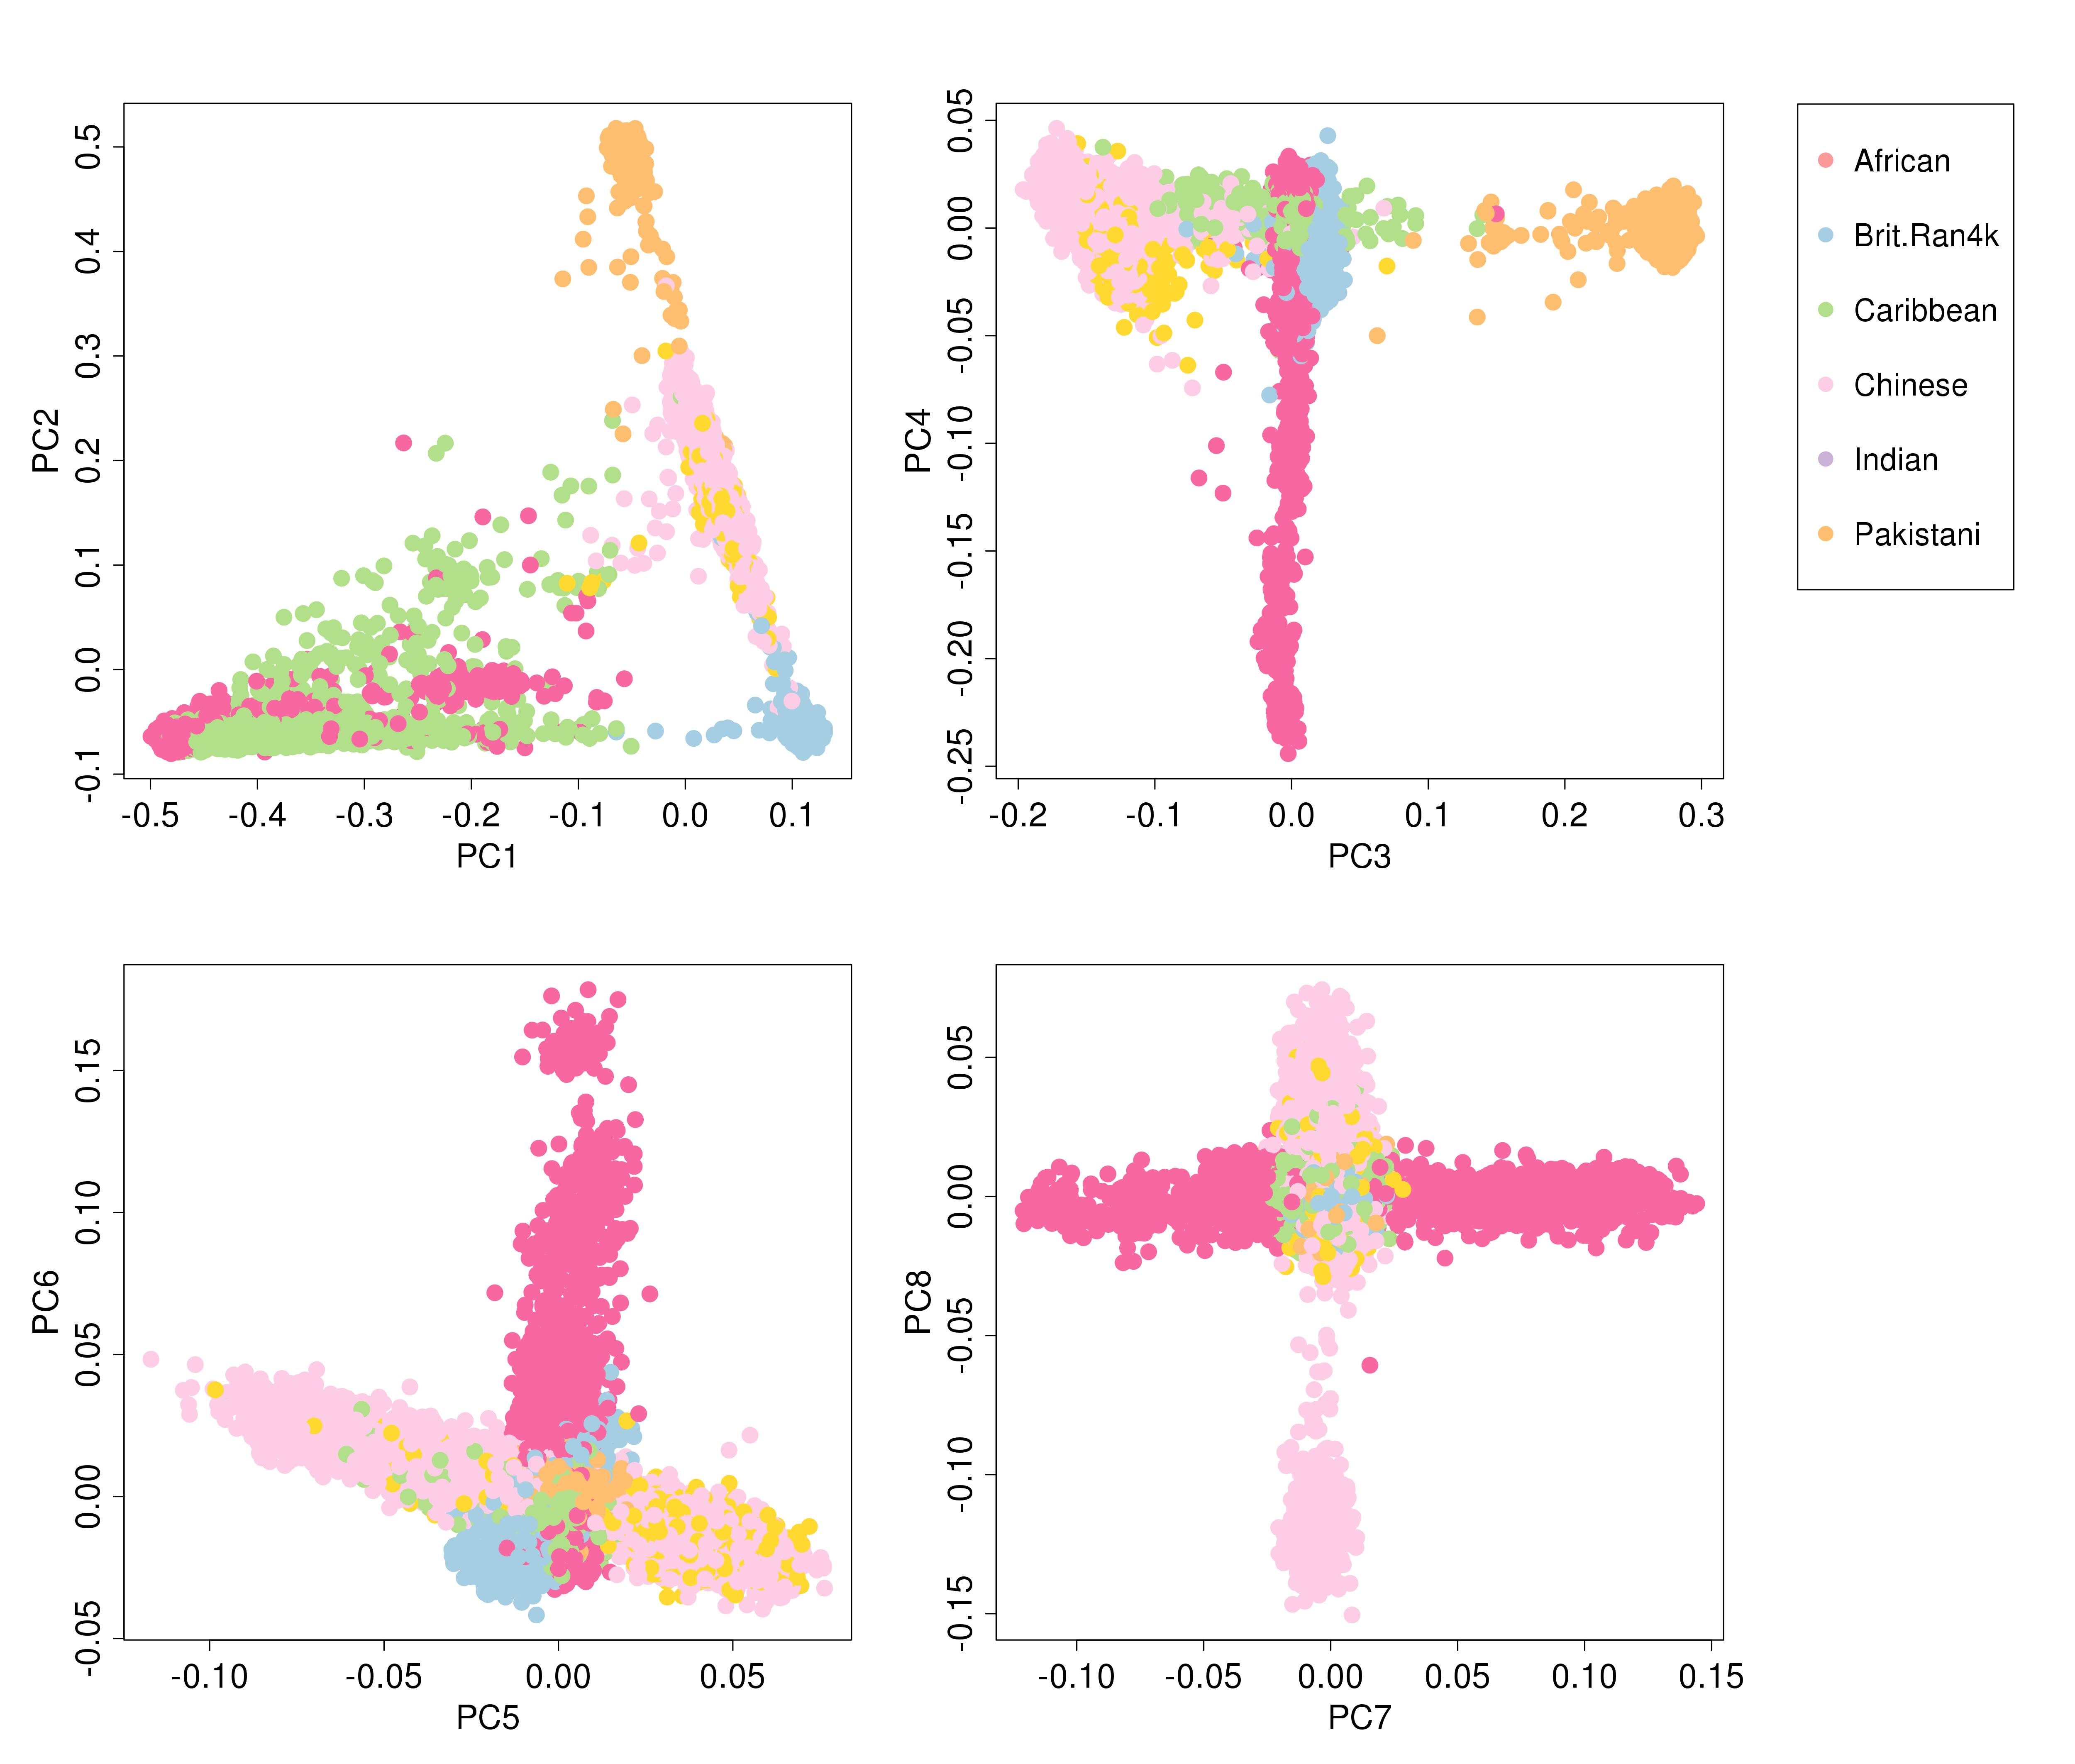
\includegraphics[scale=.4]{Images/Supp/InterPath_Supp_Figure_UKB_PCAPlot_vs1.png}
\caption[TBD]{\textbf{Global PCA Plots of the UK BioBank subgroups}. The figure shows the top 8 global principal components of our UKB subgroup dataset plotted against one another: a) PC1 vs. PC2, b) PC3 vs. PC4, c) PC5 vs. PC6, d) PC7 vs. PC8. PCA was conducted using FlashPCA \citep{Abraham2017} and a post-QC, pruned SNP set. Note that these PCs were created similar to the descriptions in `Population subgroups' of Methods and `Population Subgroup Quality Control' of Supplementary Note, but in lieu of running FlashPCA on each subgroup separately, FlashPCA was run on the full dataset together jointly. Local PCs were used for quality control and as covariates; global PCs were only used for these plots.}
\label{InterPath-Supp-Figure-UKB-subgroups-PCAPlot}
\end{figure}
\clearpage

\begin{figure}[htbp]
\centering
\hspace*{-1.7cm}
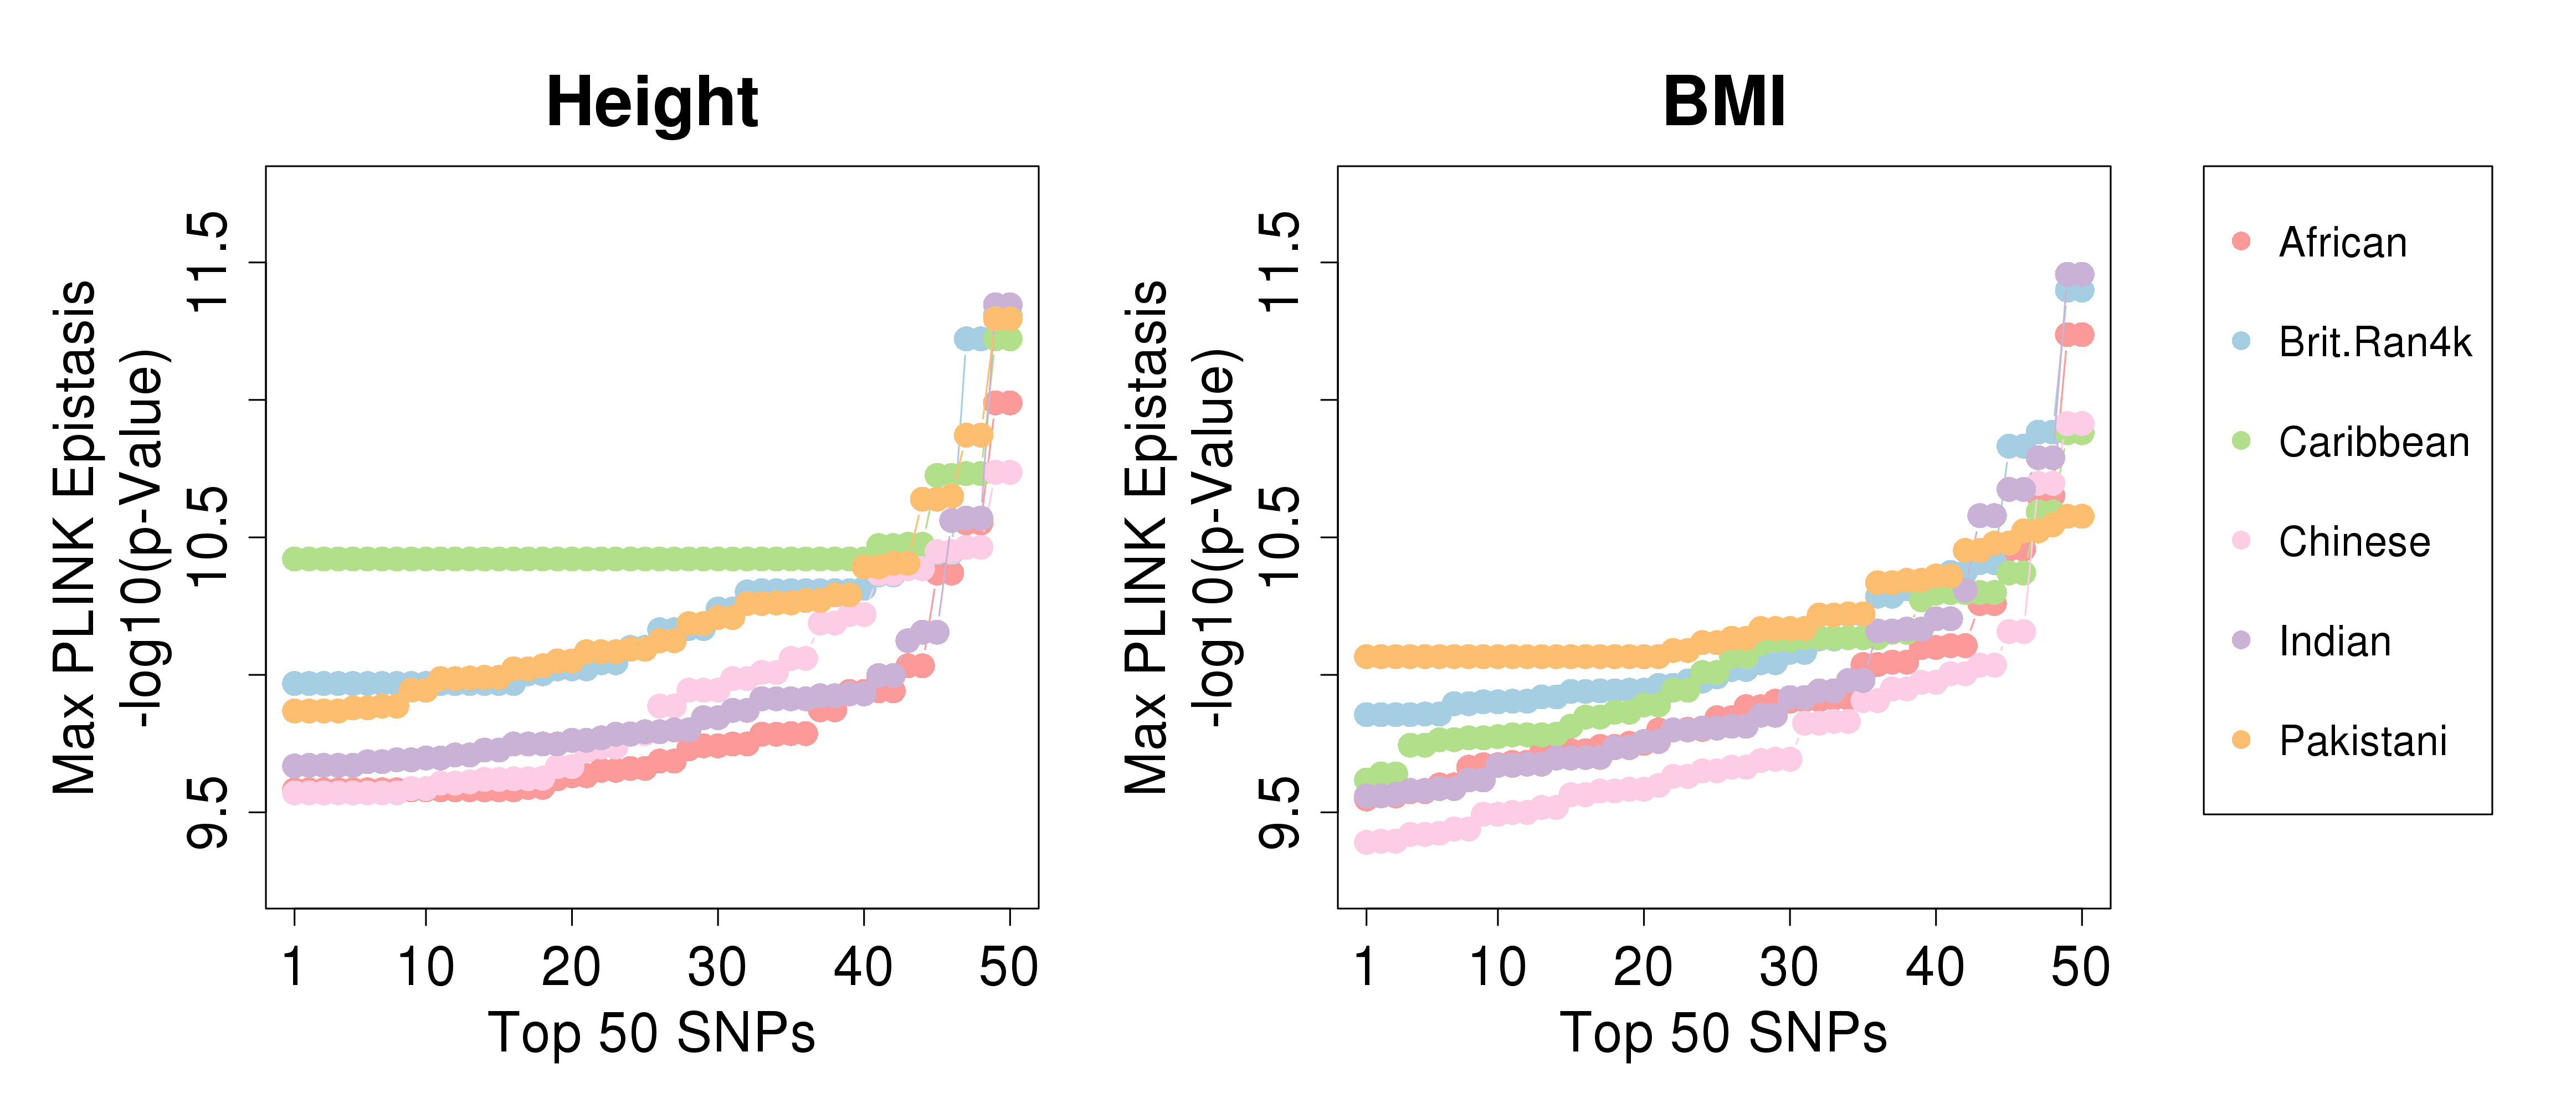
\includegraphics[scale=.45]{Images/Supp/InterPath_Supp_Figure_PLINK_BestSNPs_vs2_AllPops_HeightBMI.png}
\caption[TBD]{\textbf{SNPs with the largest PLINK pairwise epistasis signals, per subgroup}. The figure shows the best $p$-values obtained from running PLINK's exhaustive pairwise SNP epistasis test for both height and BMI in each of the UKB subgroups. Only the top 50 SNPs, sorted by best pairwise SNP epistasis $p$-value, for each subgroup are shown. No test reaches genome-wide significance based on using a Bonferroni-corrected $p$-value threshold ($p$-value $< 5\times10^{-13}$).}
\label{InterPath-Supp-Figure-PLINK-HeightBMI-AllPops}
\end{figure}
\clearpage

%\begin{figure}[htbp]
%\centering
%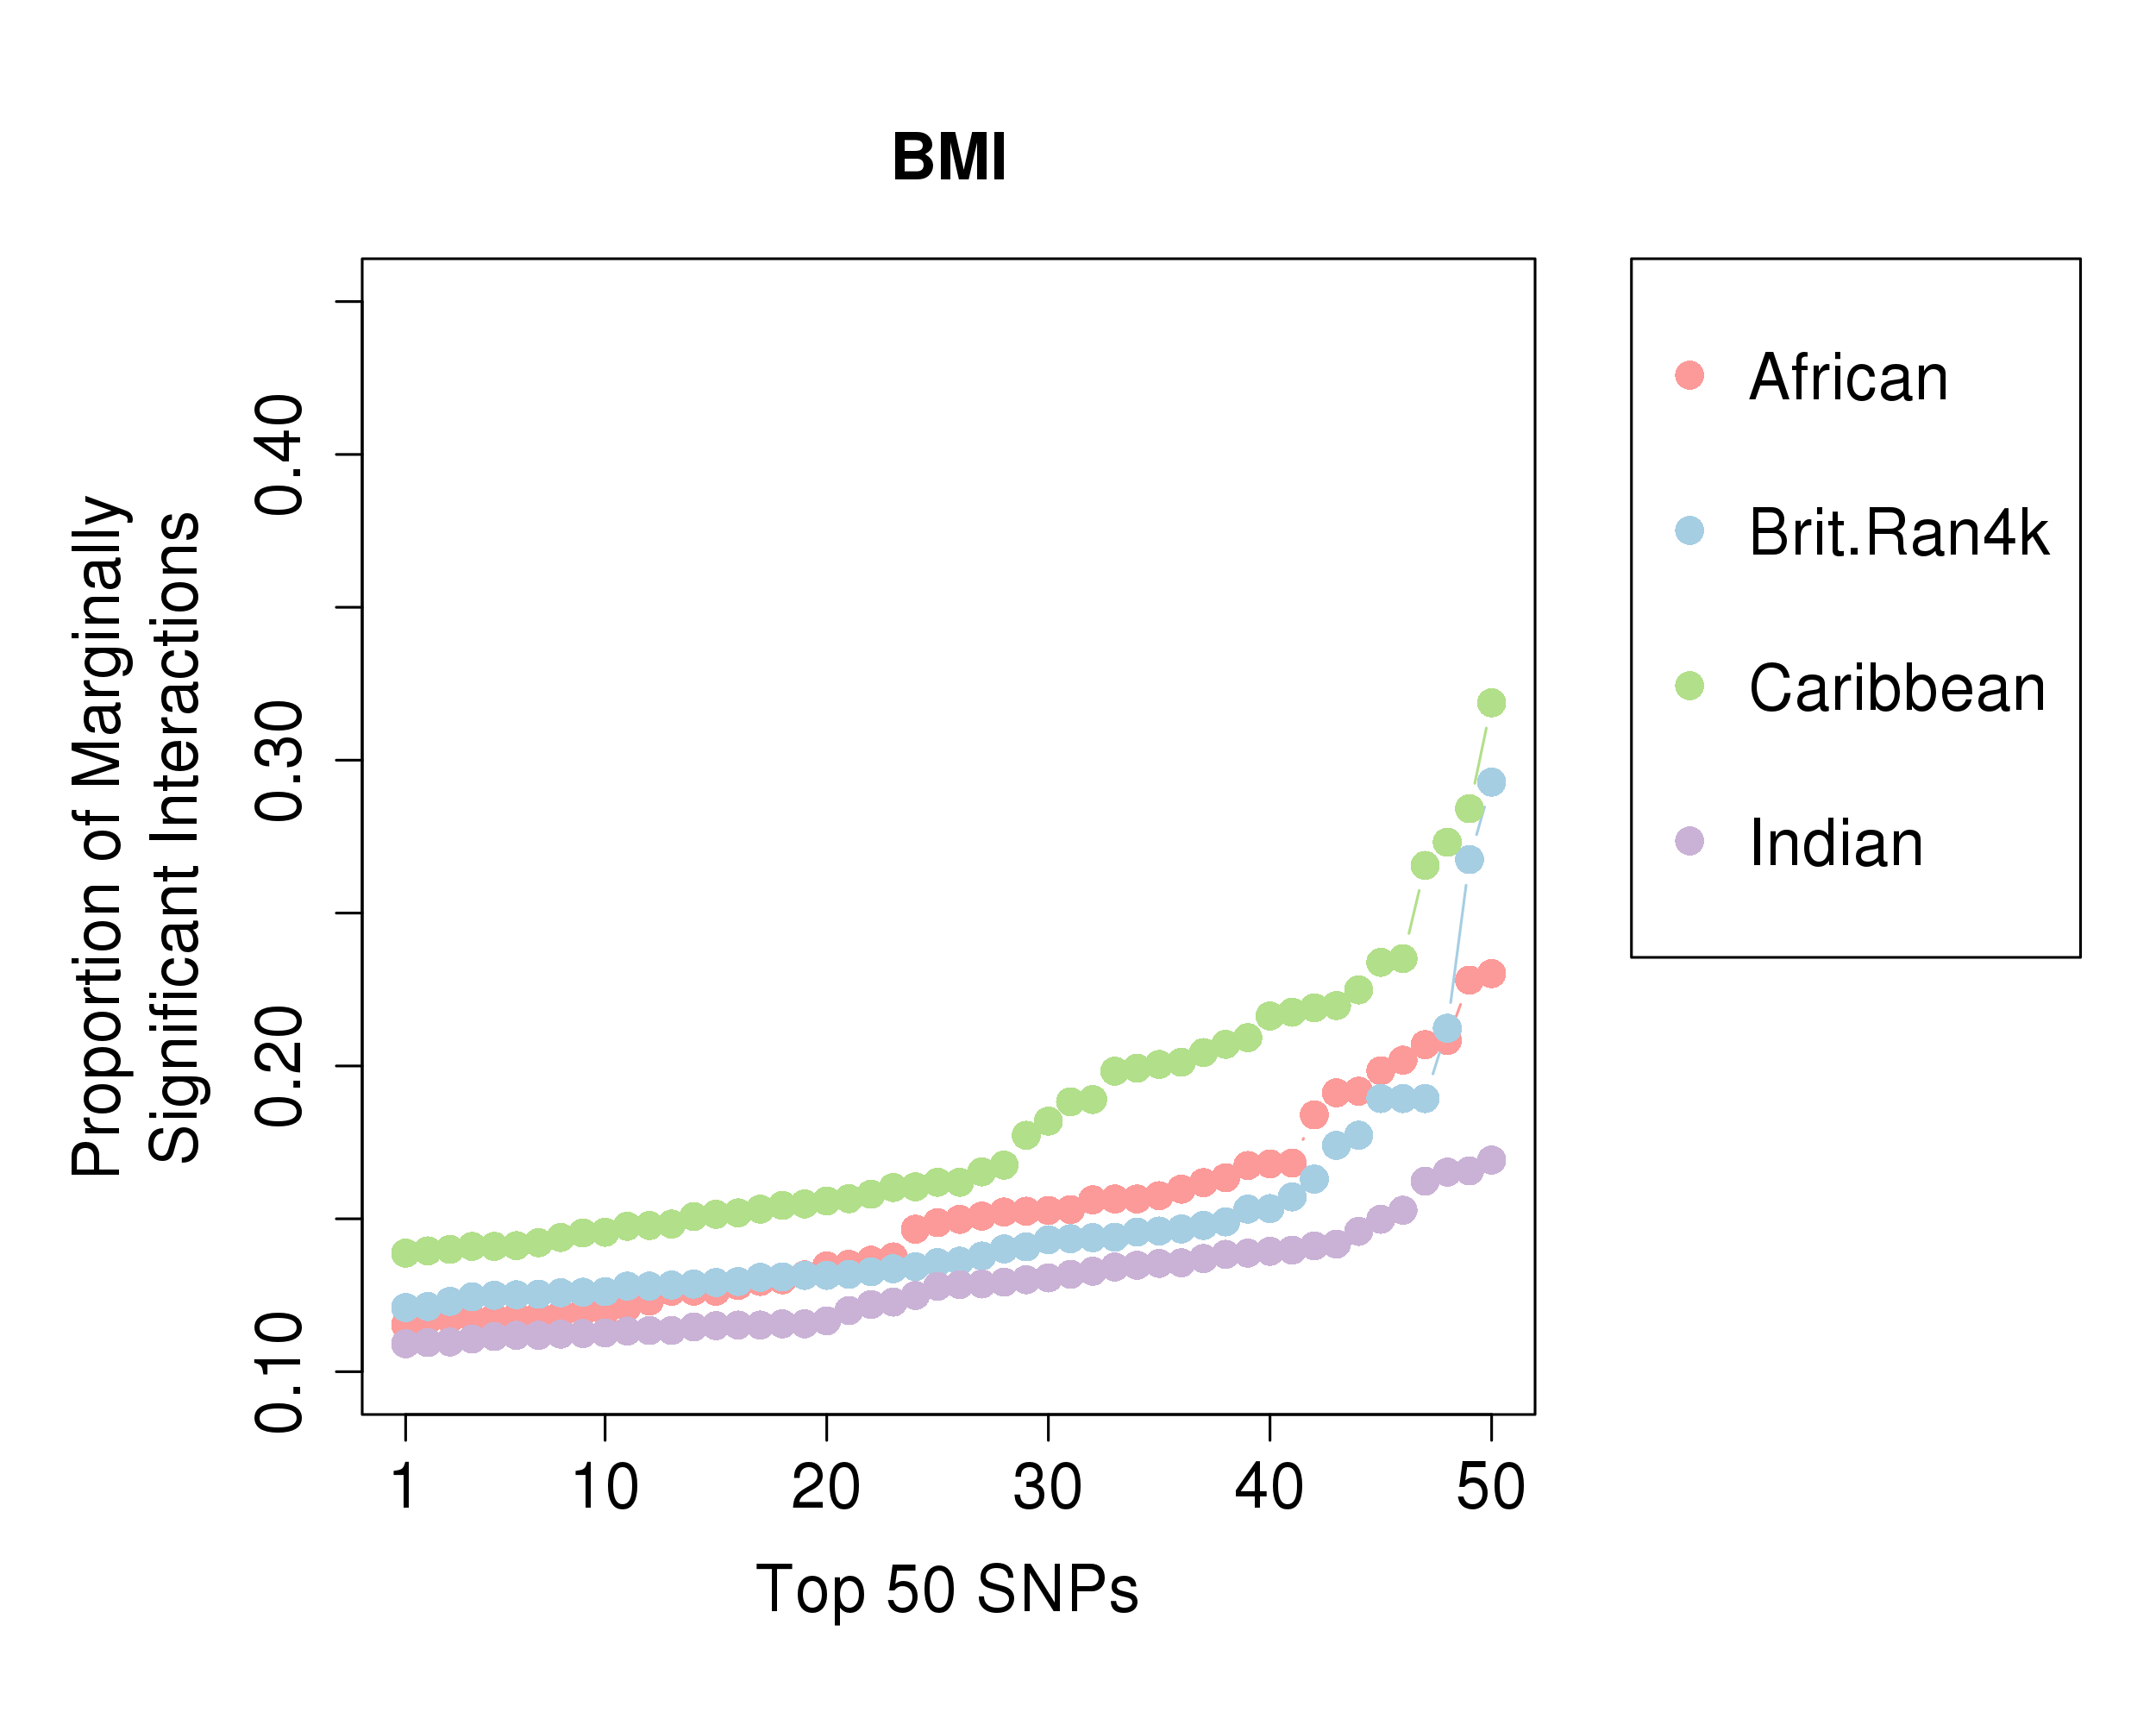
\includegraphics[scale=.5]{Images/Supp/InterPath_Supp_Figure_PLINK_vs3_BMI.png}
%\caption[TBD]{\textbf{PLINK Epistasis Proportion Results: BMI}. The figure shows the proportion of pairwise marginally significant epistatic interactions a single SNP contains when tested on height within our UKB subgroups. Pairwise tests are conducted exhaustively for each individual SNP through PLINK. Marginally significant is defined as pairwise SNP epistasis $p$-value $< 1\times10^{-4}$. Only the top 50 SNPs sorted by decreasing proportion are shown for each UKB subgroup. For results on height see Figure \ref{InterPath-Main-Figure-PLINK-Proportions-Height}. In general we find that the African and Caribbean subgroups have the highest proportions of marginally significant interactions per SNP.}
%\label{InterPath-Supp-Figure-PLINK-Proportions-BMI}
%\end{figure}

\begin{figure}[htb]
\centering
\hspace*{-1.7cm}
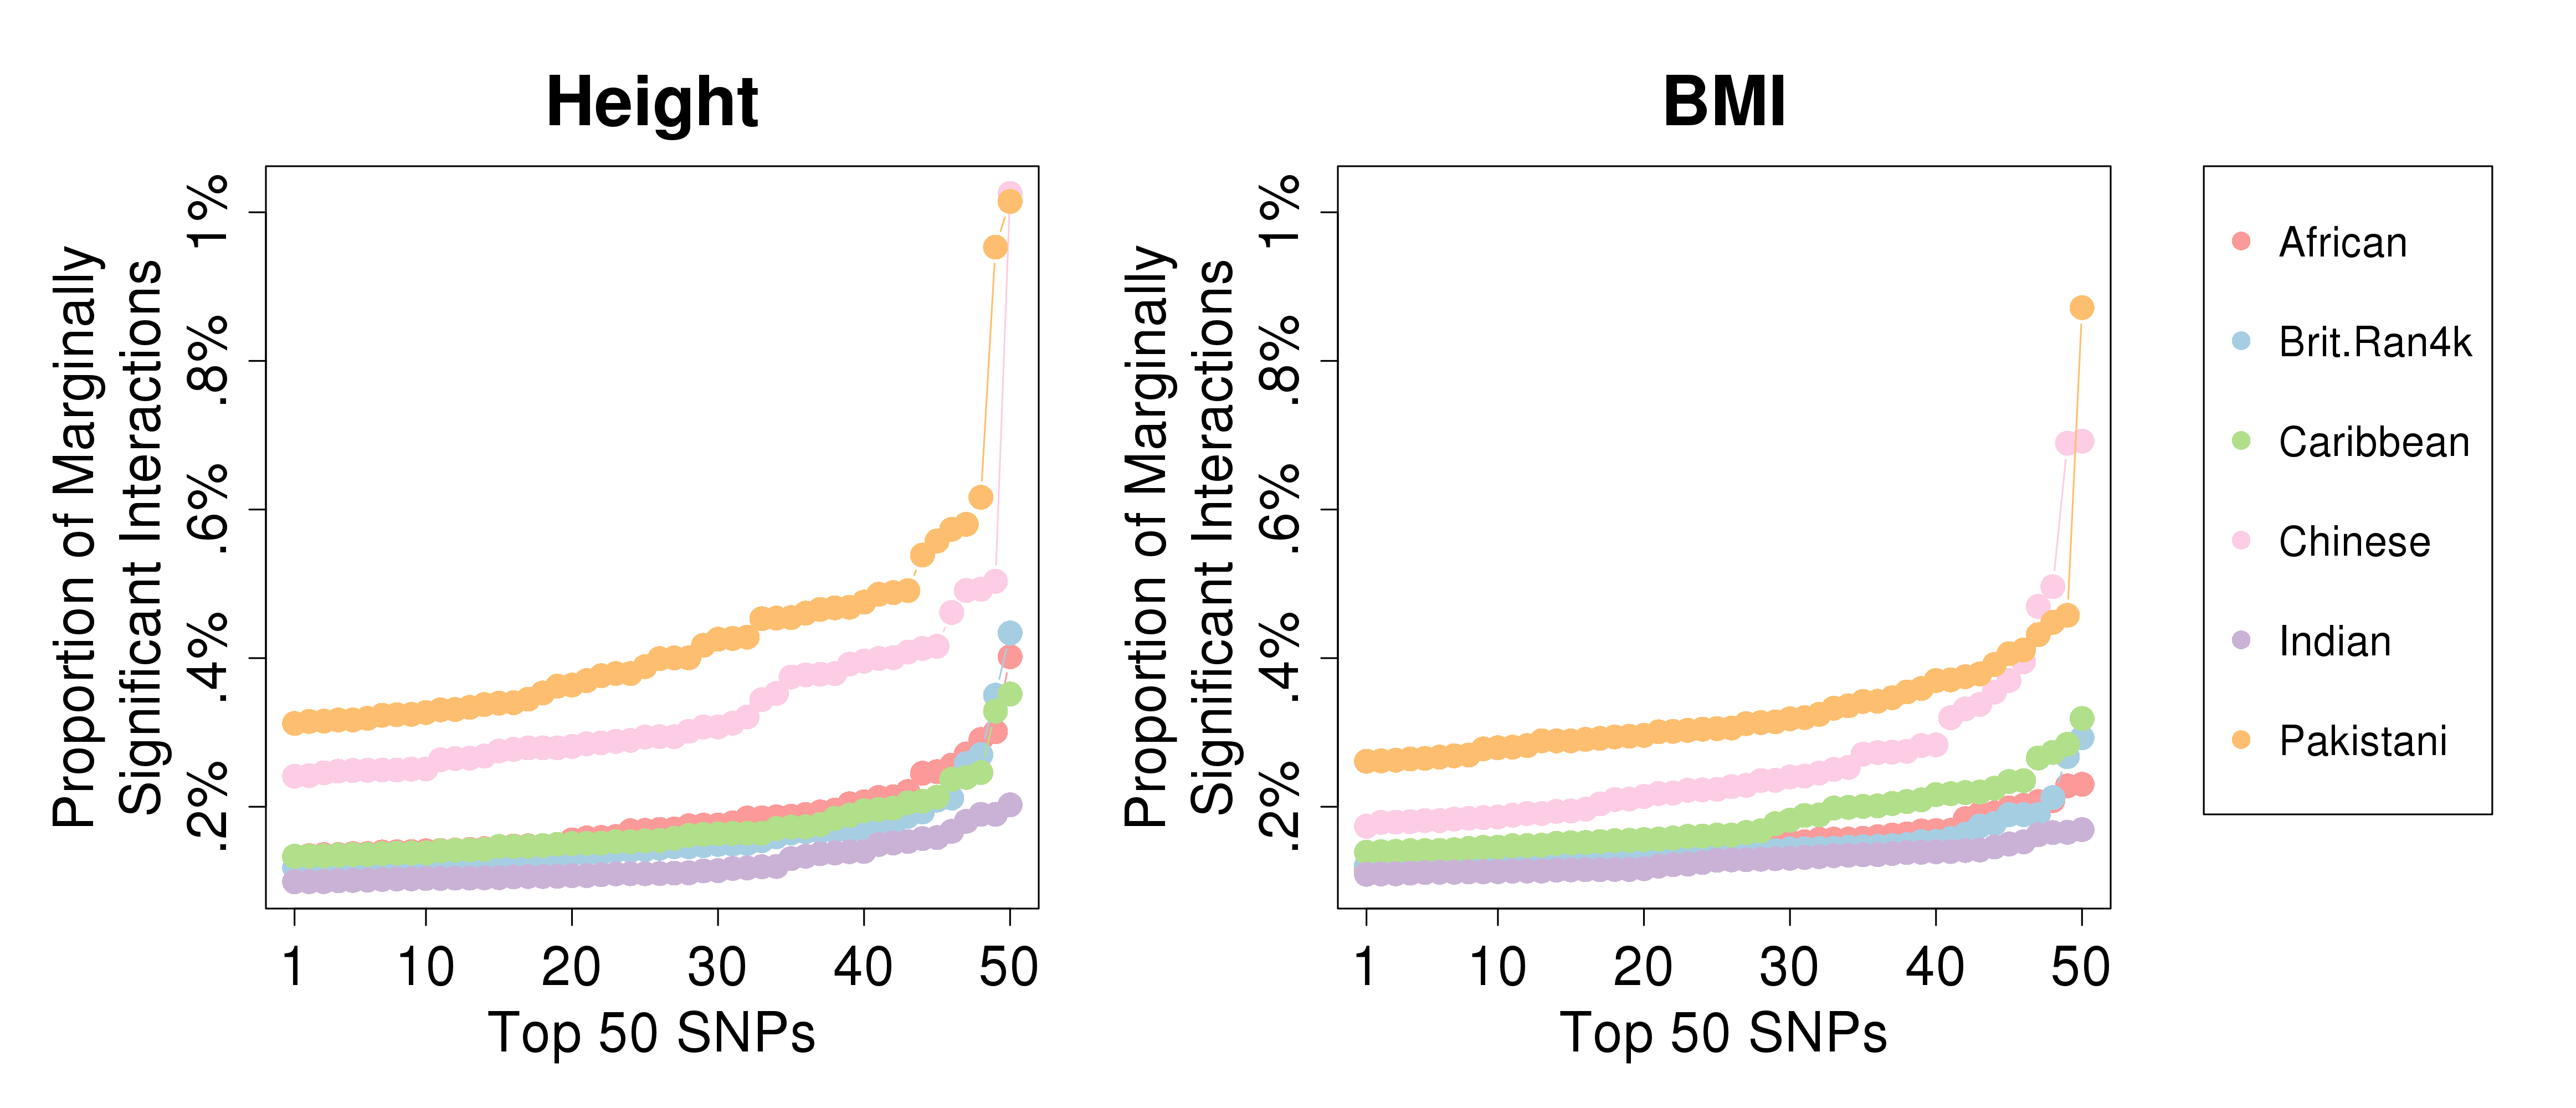
\includegraphics[scale=.45]{Images/Main/InterPath_Main_Figure_PLINK_vs4_HeightBMI.png}
\caption[TBD]{\textbf{SNPs with the largest proportions of marginally significant PLINK pairwise epistasis tests, per subgroup}. The figure shows the proportion of pairwise marginally significant epistatic interactions a single SNP contains when tested on height and BMI within our UKB subgroups. Pairwise tests are conducted exhaustively for each individual SNP through PLINK. Marginally significant is defined as a pairwise SNP epistasis $p$-value $< 1\times10^{-4}$. Only the top 50 SNPs sorted by decreasing proportion are shown for each UKB subgroup. In general we find that the African and Caribbean subgroups have the highest proportions of marginally significant interactions per SNP.}
\label{InterPath-Supp-Figure-PLINK-Proportions-HeightBMI}
\end{figure}

%\begin{figure}[htbp]
%\centering
%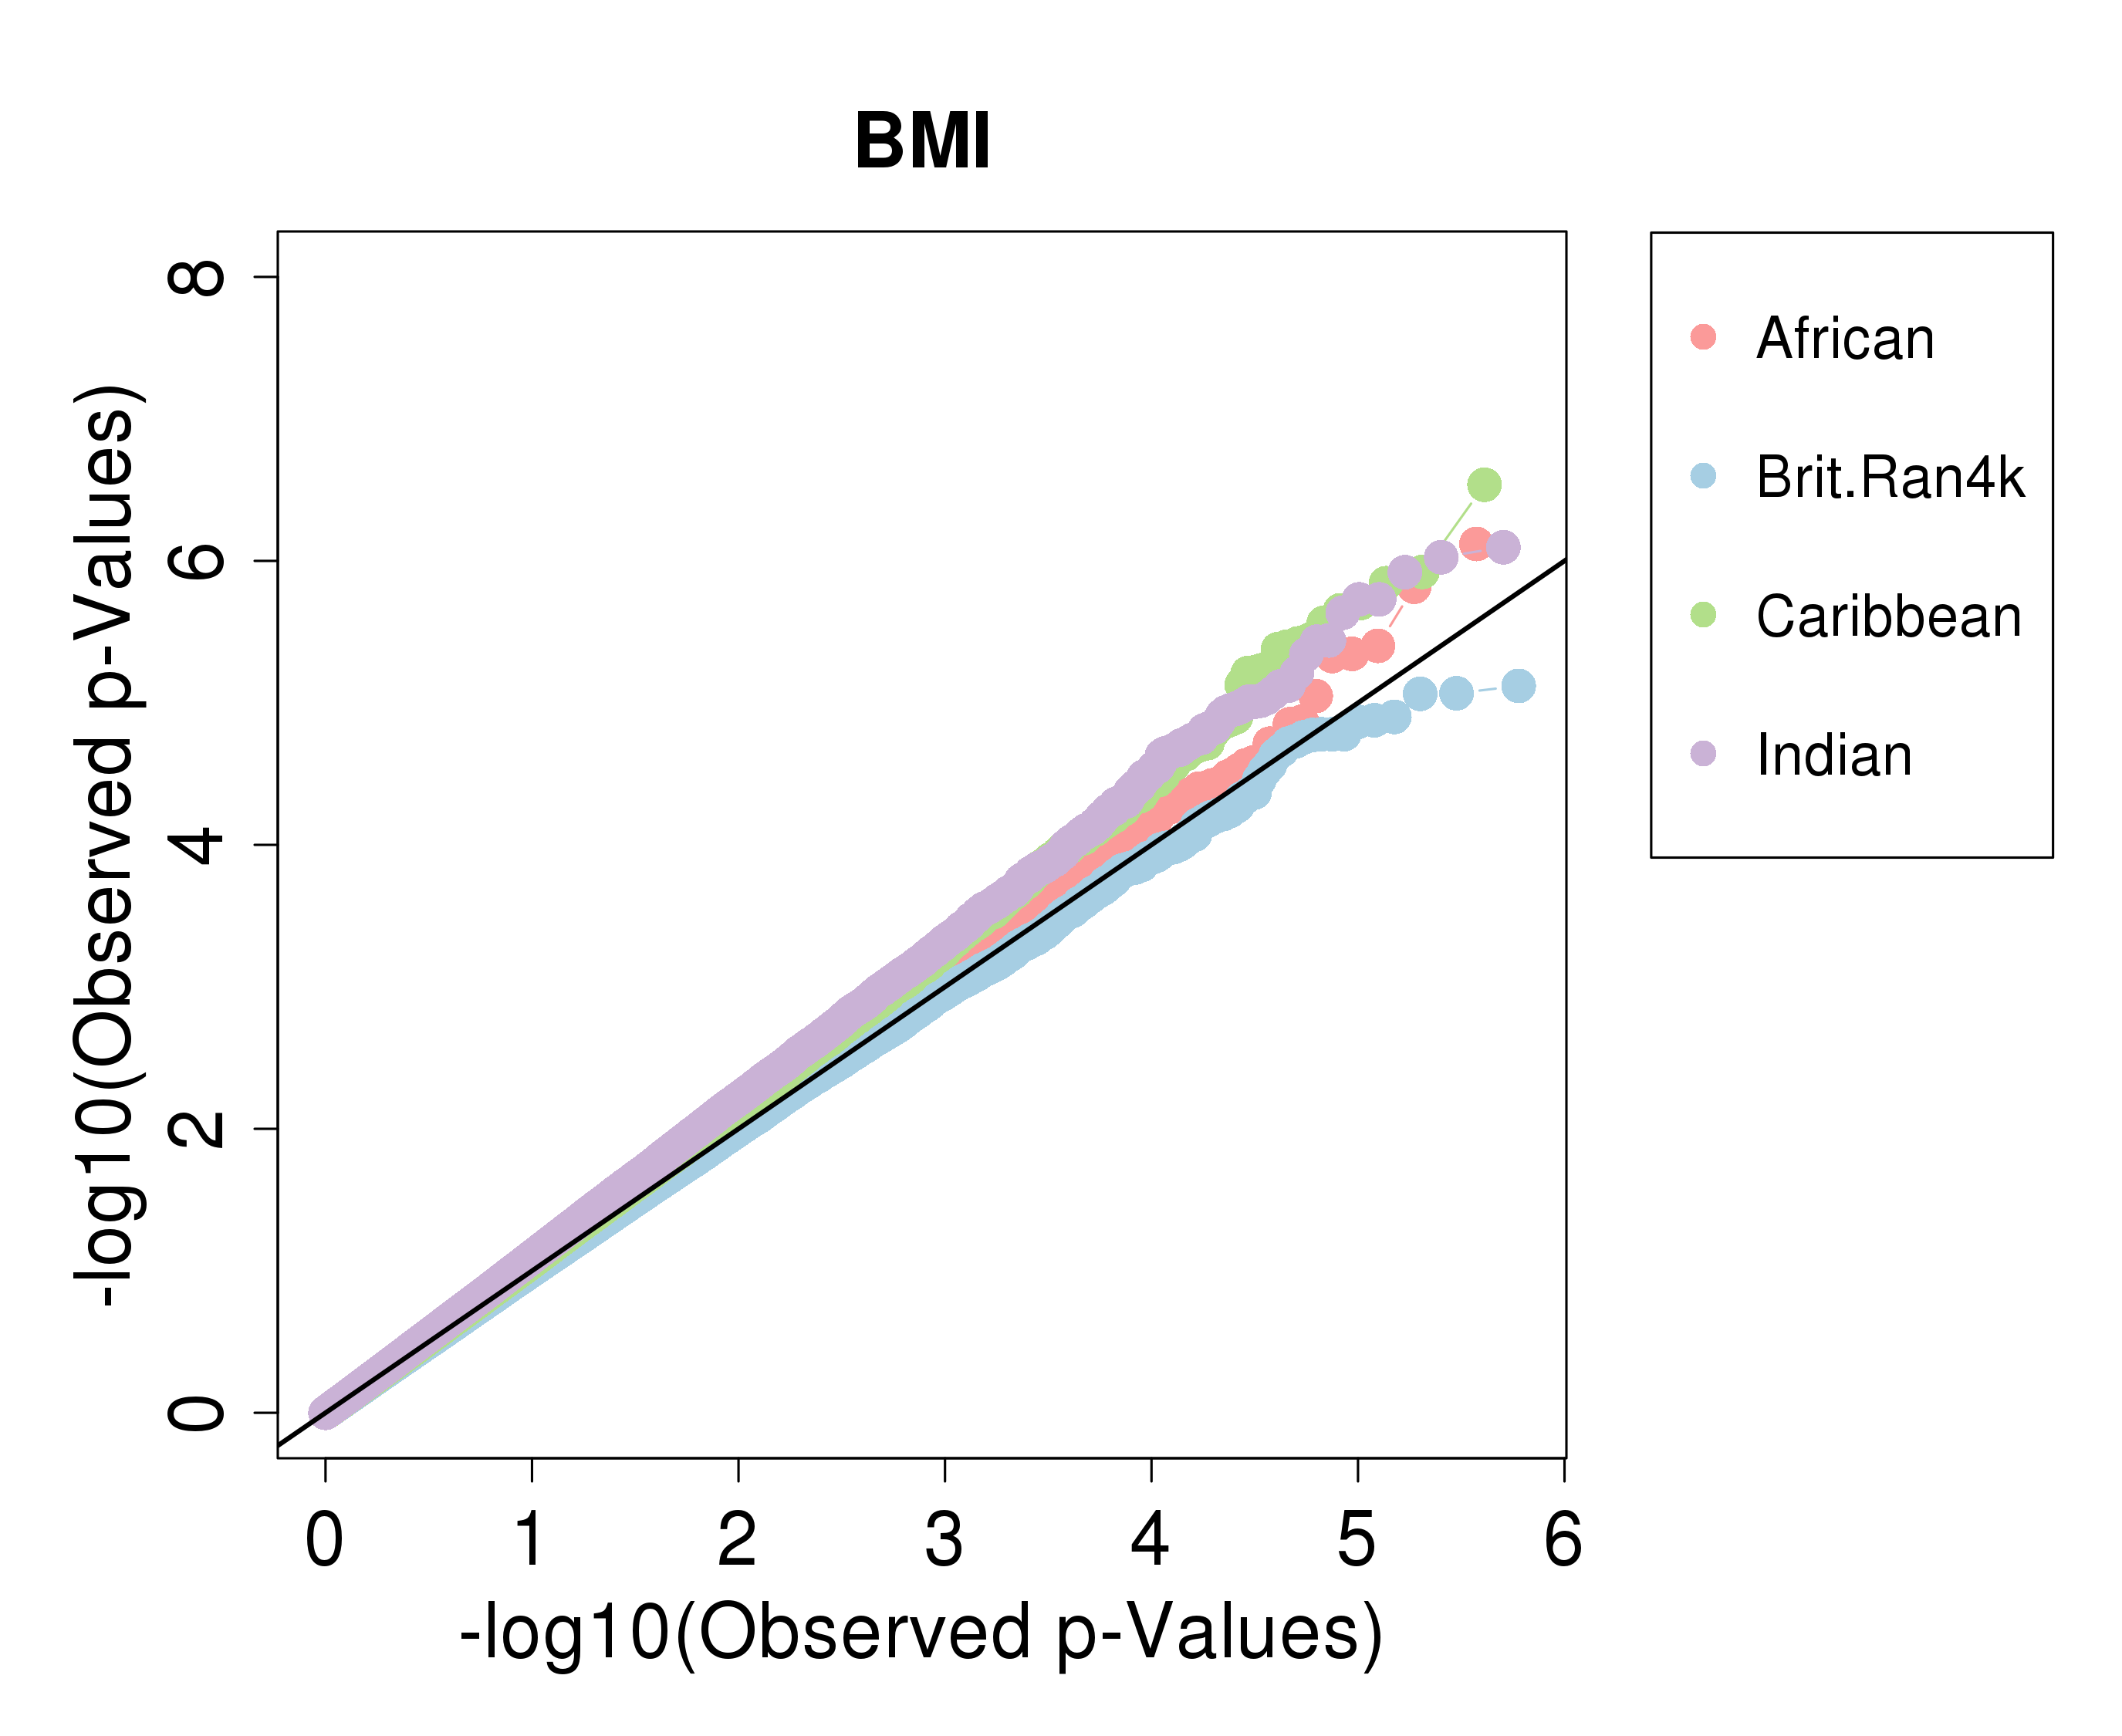
\includegraphics[scale=.5]{Images/Supp/InterPath_Supp_Figure_MAPIT_vs3_BMI.png}
%\caption[TBD]{\textbf{MAPIT Results: BMI QQ-Plots}. The figure shows QQ-plots of our results from running MAPIT on our four initial UKB population subgroups in BMI. On the $x$-axis are the -$\log_{10}$ of the expected $p$-values and the on the $y$-axis are on the -$\log_{10}$ of the observed $p$-values. Each data point is a SNP and total SNP counts per UKB subgroup can be found in Supplementary Table \ref{InterPath-Supp-Table-UKBPopStats}.}
%\label{InterPath-Supp-Figure-MAPIT-BMI}
%\end{figure}
%\clearpage

\begin{figure}[htb]
\centering
\hspace*{-1.4cm}
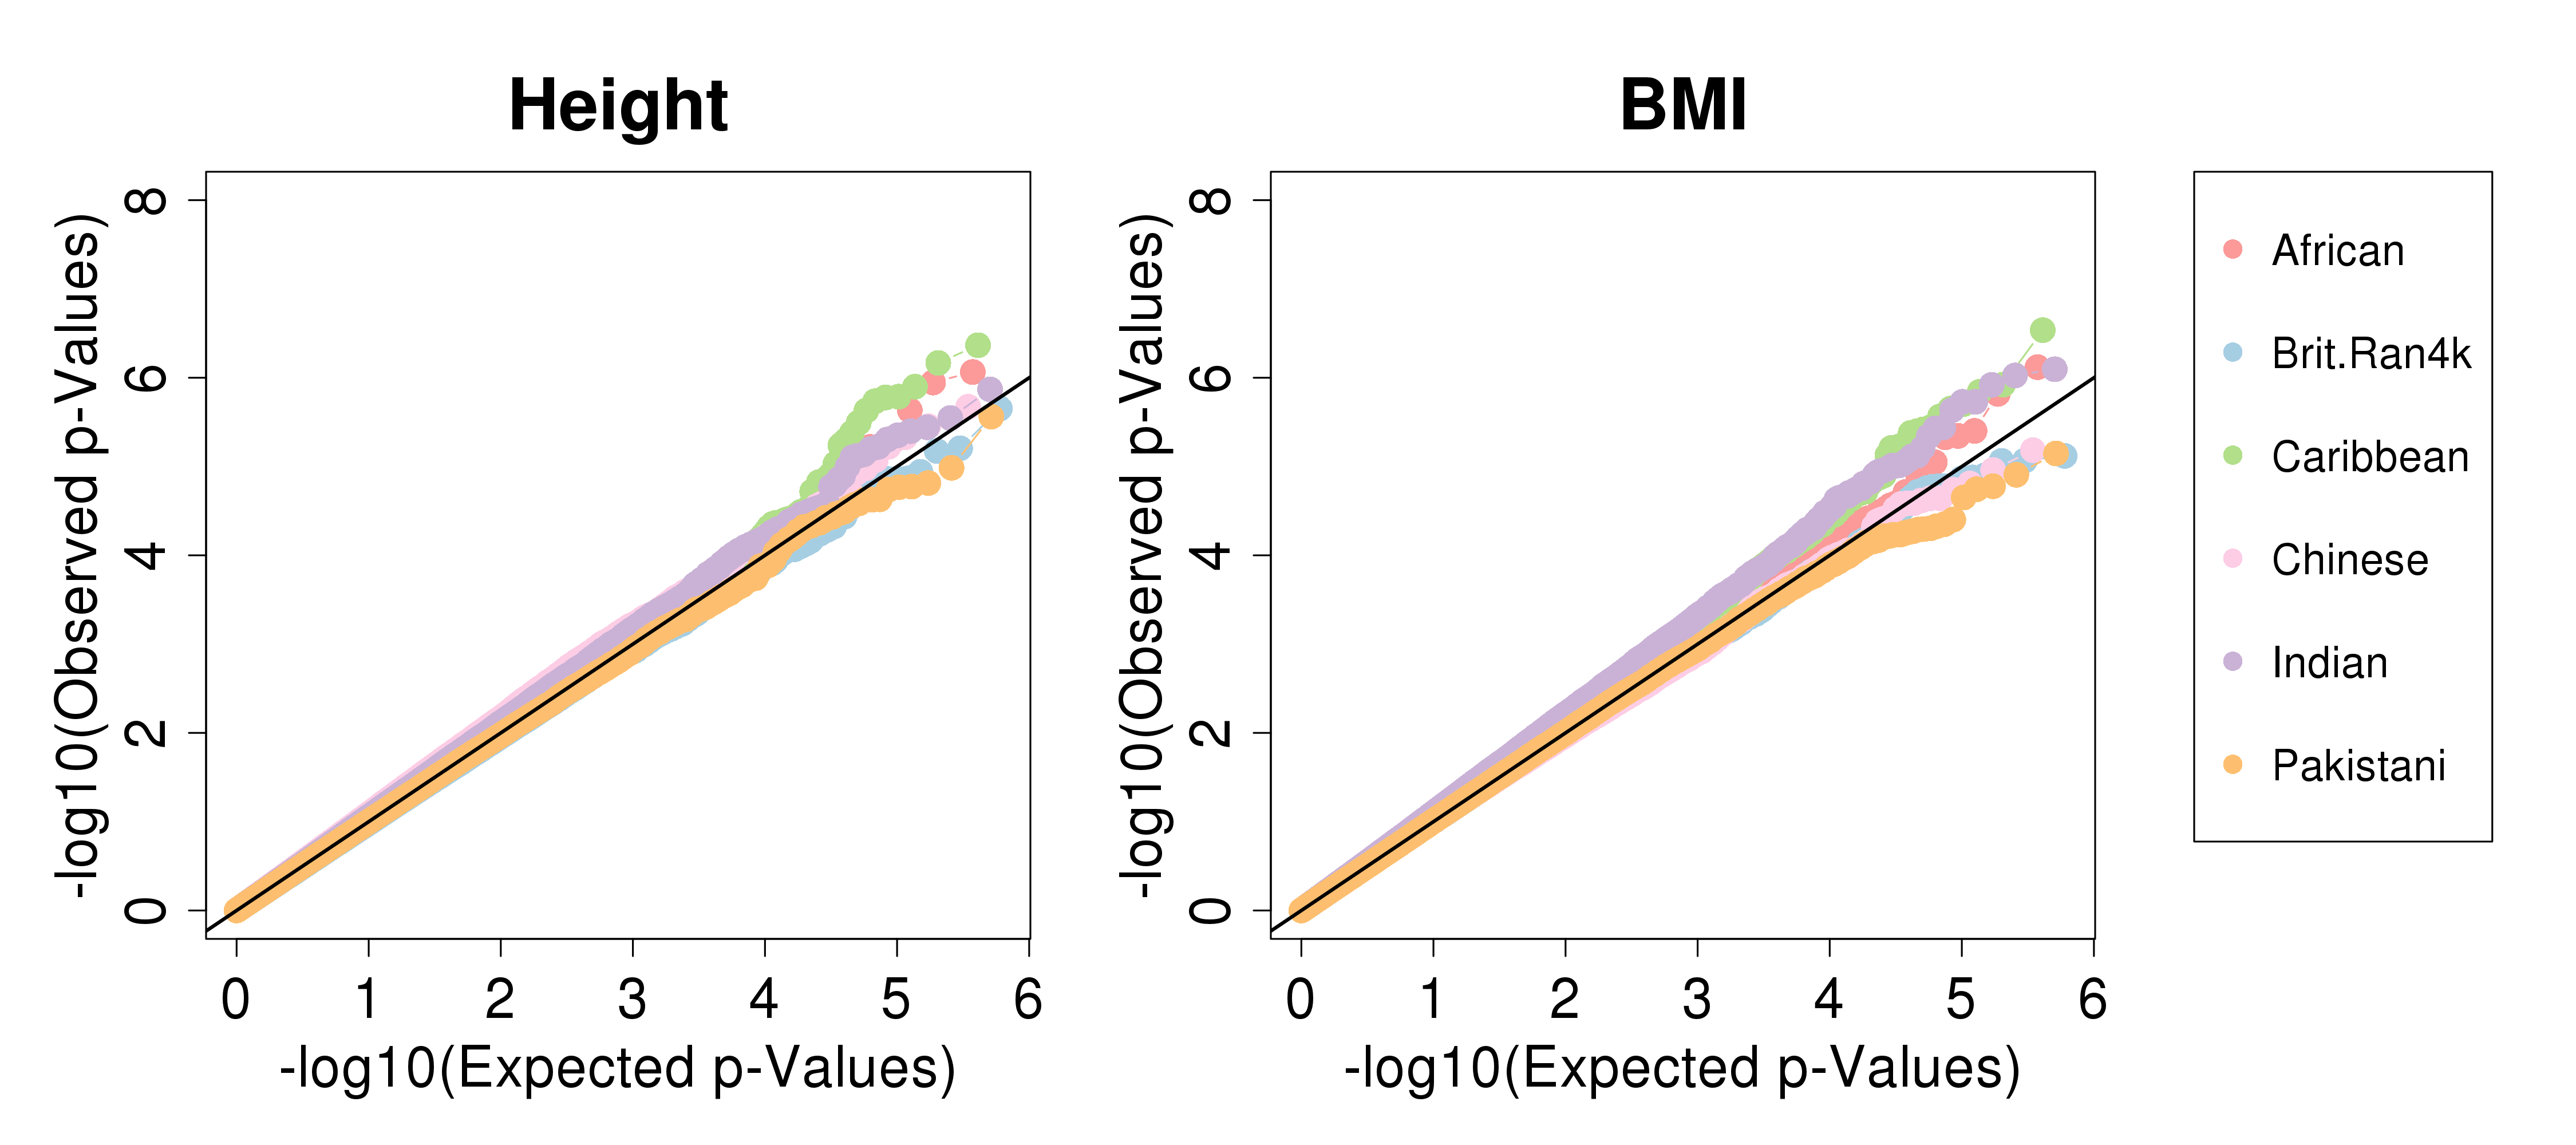
\includegraphics[scale=.45]{Images/Main/InterPath_Main_Figure_MAPIT_vs4_HeightBMI.png}
\caption[TBD]{\textbf{QQ-Plots of MAPIT results, per subgroup}. The figure shows QQ-plots of our results from running MAPIT on our four initial UKB population subgroups in height and BMI. On the $x$-axis are the -$\log_{10}$ of the expected $p$-values and the on the $y$-axis are on the -$\log_{10}$ of the observed $p$-values. Each data point is a SNP and total SNP counts per UKB subgroup can be found in Supplementary Table \ref{InterPath-Supp-Table-UKBPopStats}. We observe no genome-wide significant signals in any subgroup across both phenotypes ($p$-value $< 5\times10^{-8}$) and, due to this lack of significant results, observe no clear differences in patterns between our subgroups.}
\label{InterPath-Supp-Figure-MAPIT-HeightBMI}
\end{figure}

%\begin{figure}[htbp]
%\centering
%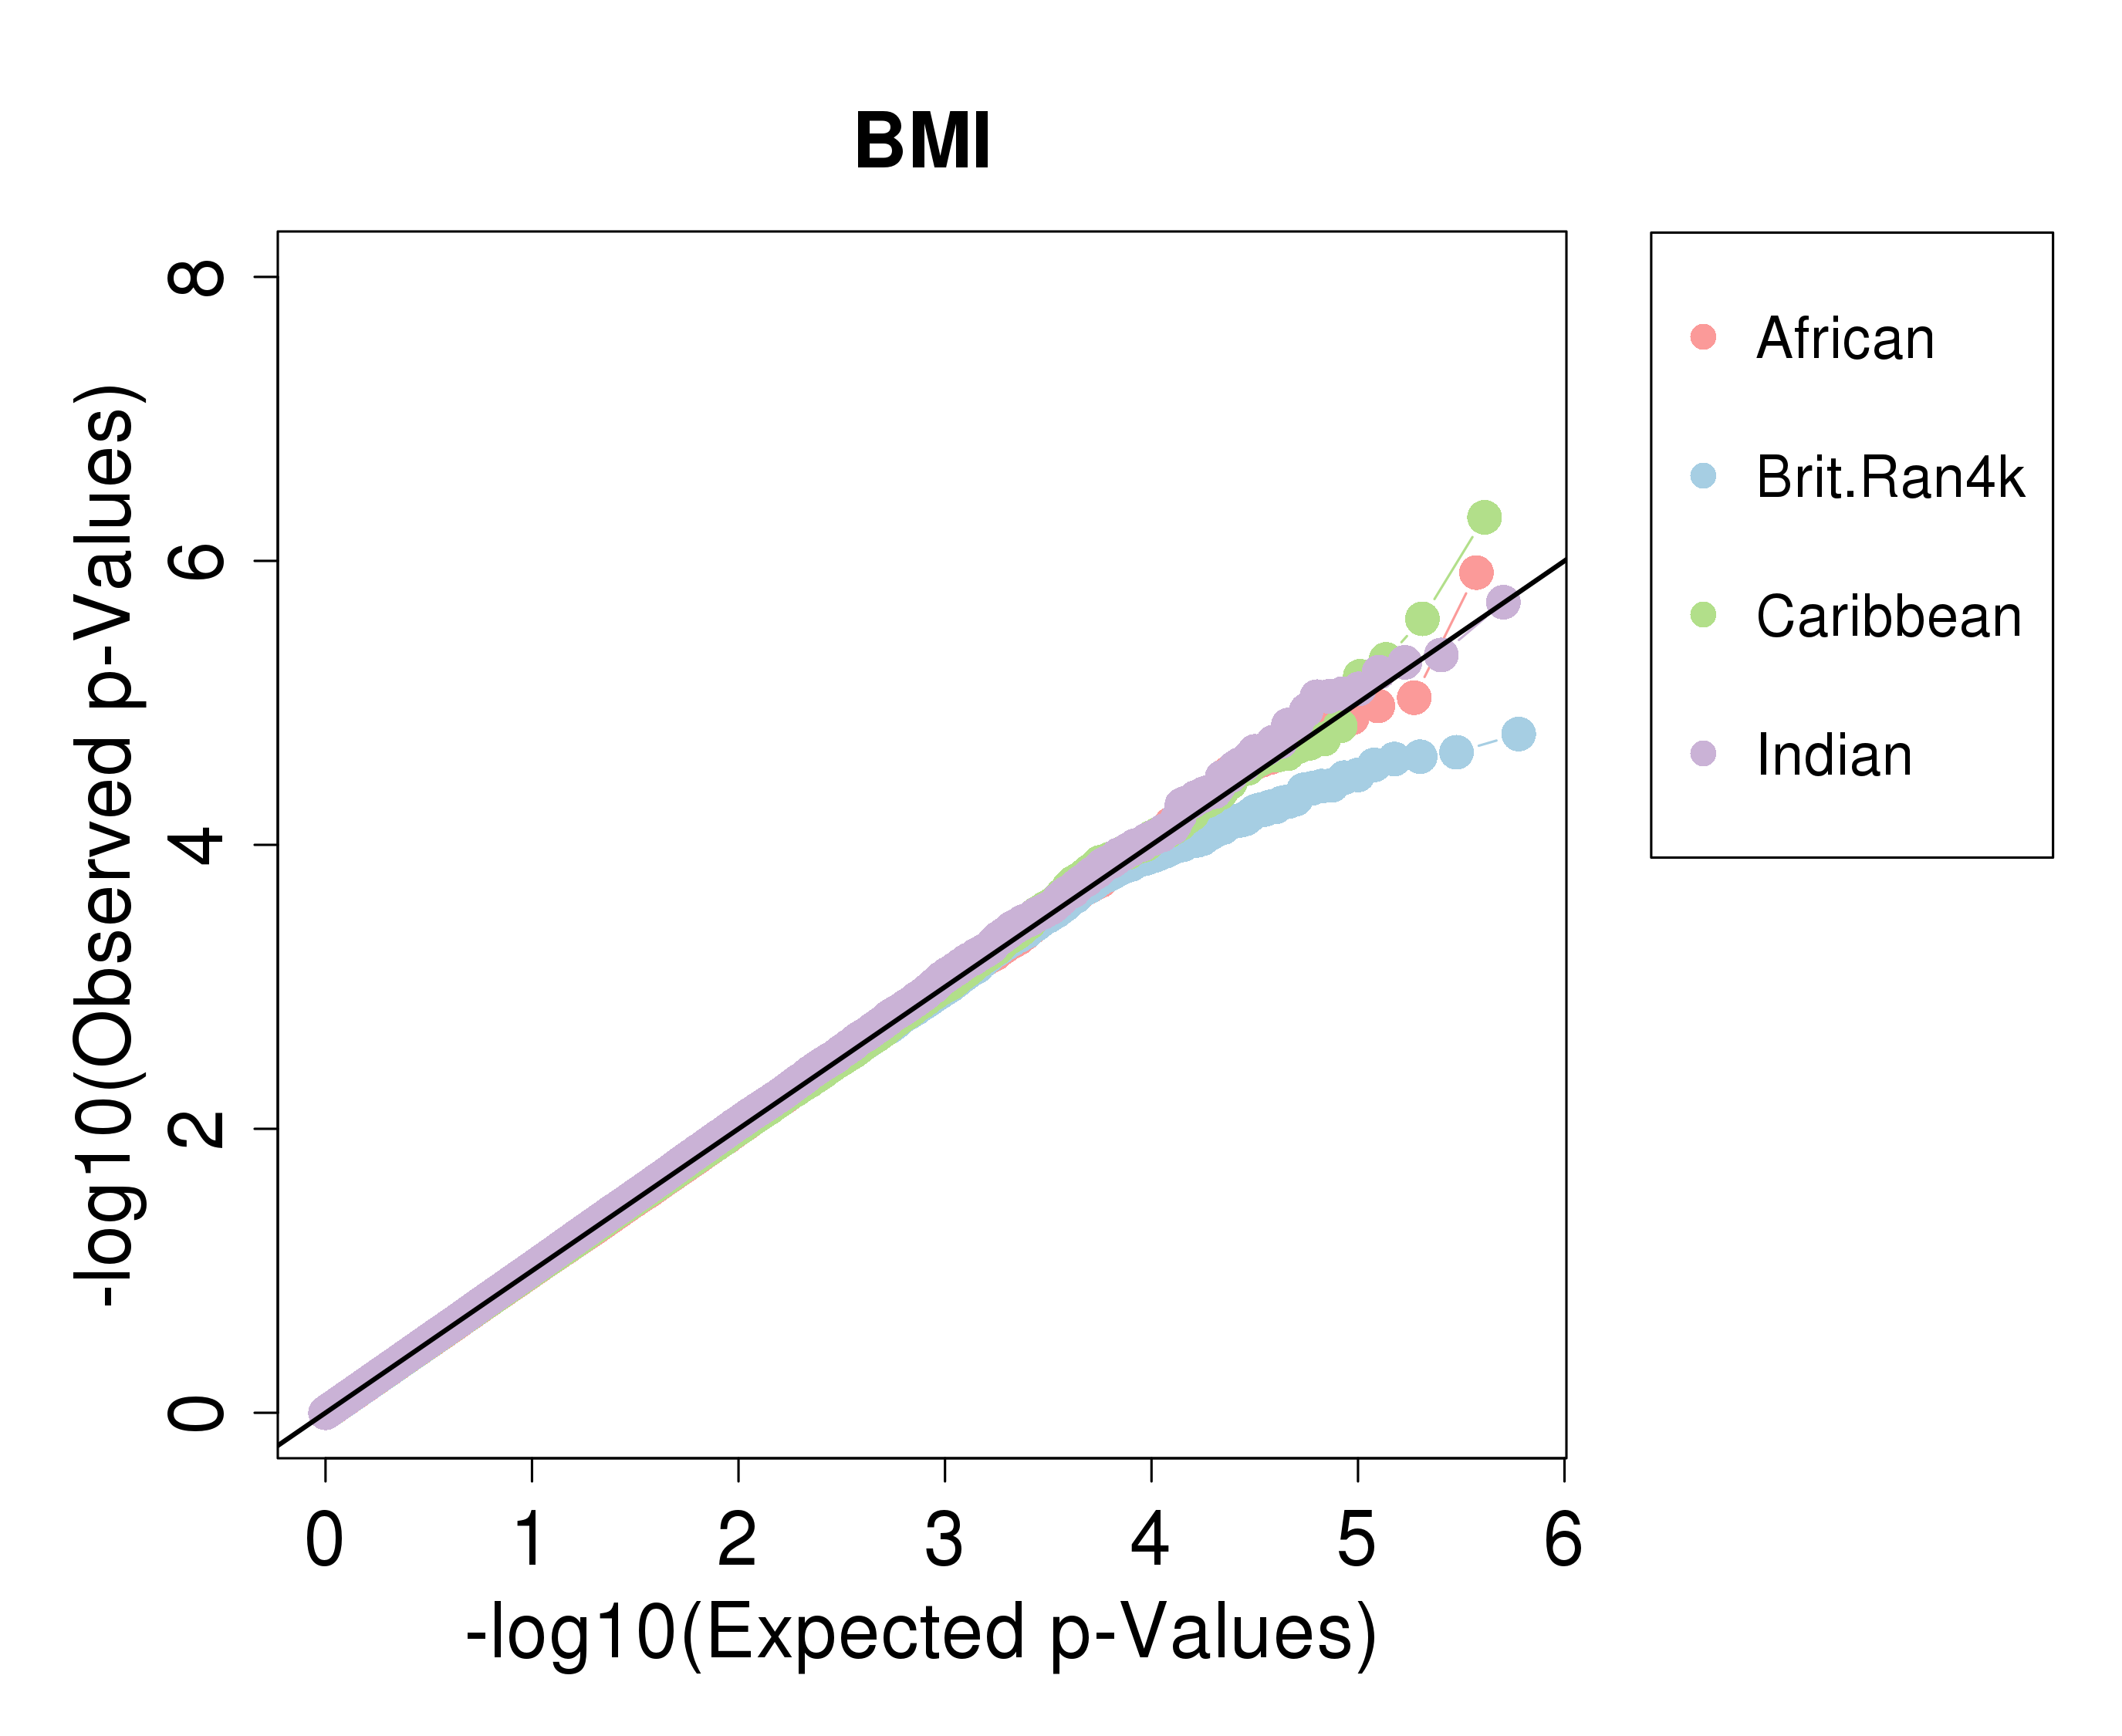
\includegraphics[scale=.35]{Images/Supp/InterPath_Supp_Figure_GWAS_vs2_BMI.png}
%\caption[TBD]{\textbf{GWAS Results QQ-Plots}.}
%\label{InterPath-Supp-Figure-GWAS-BMI}
%\end{figure}
%\clearpage
%
%\begin{figure}[htbp]
%\centering
%\hspace*{-.75cm}
%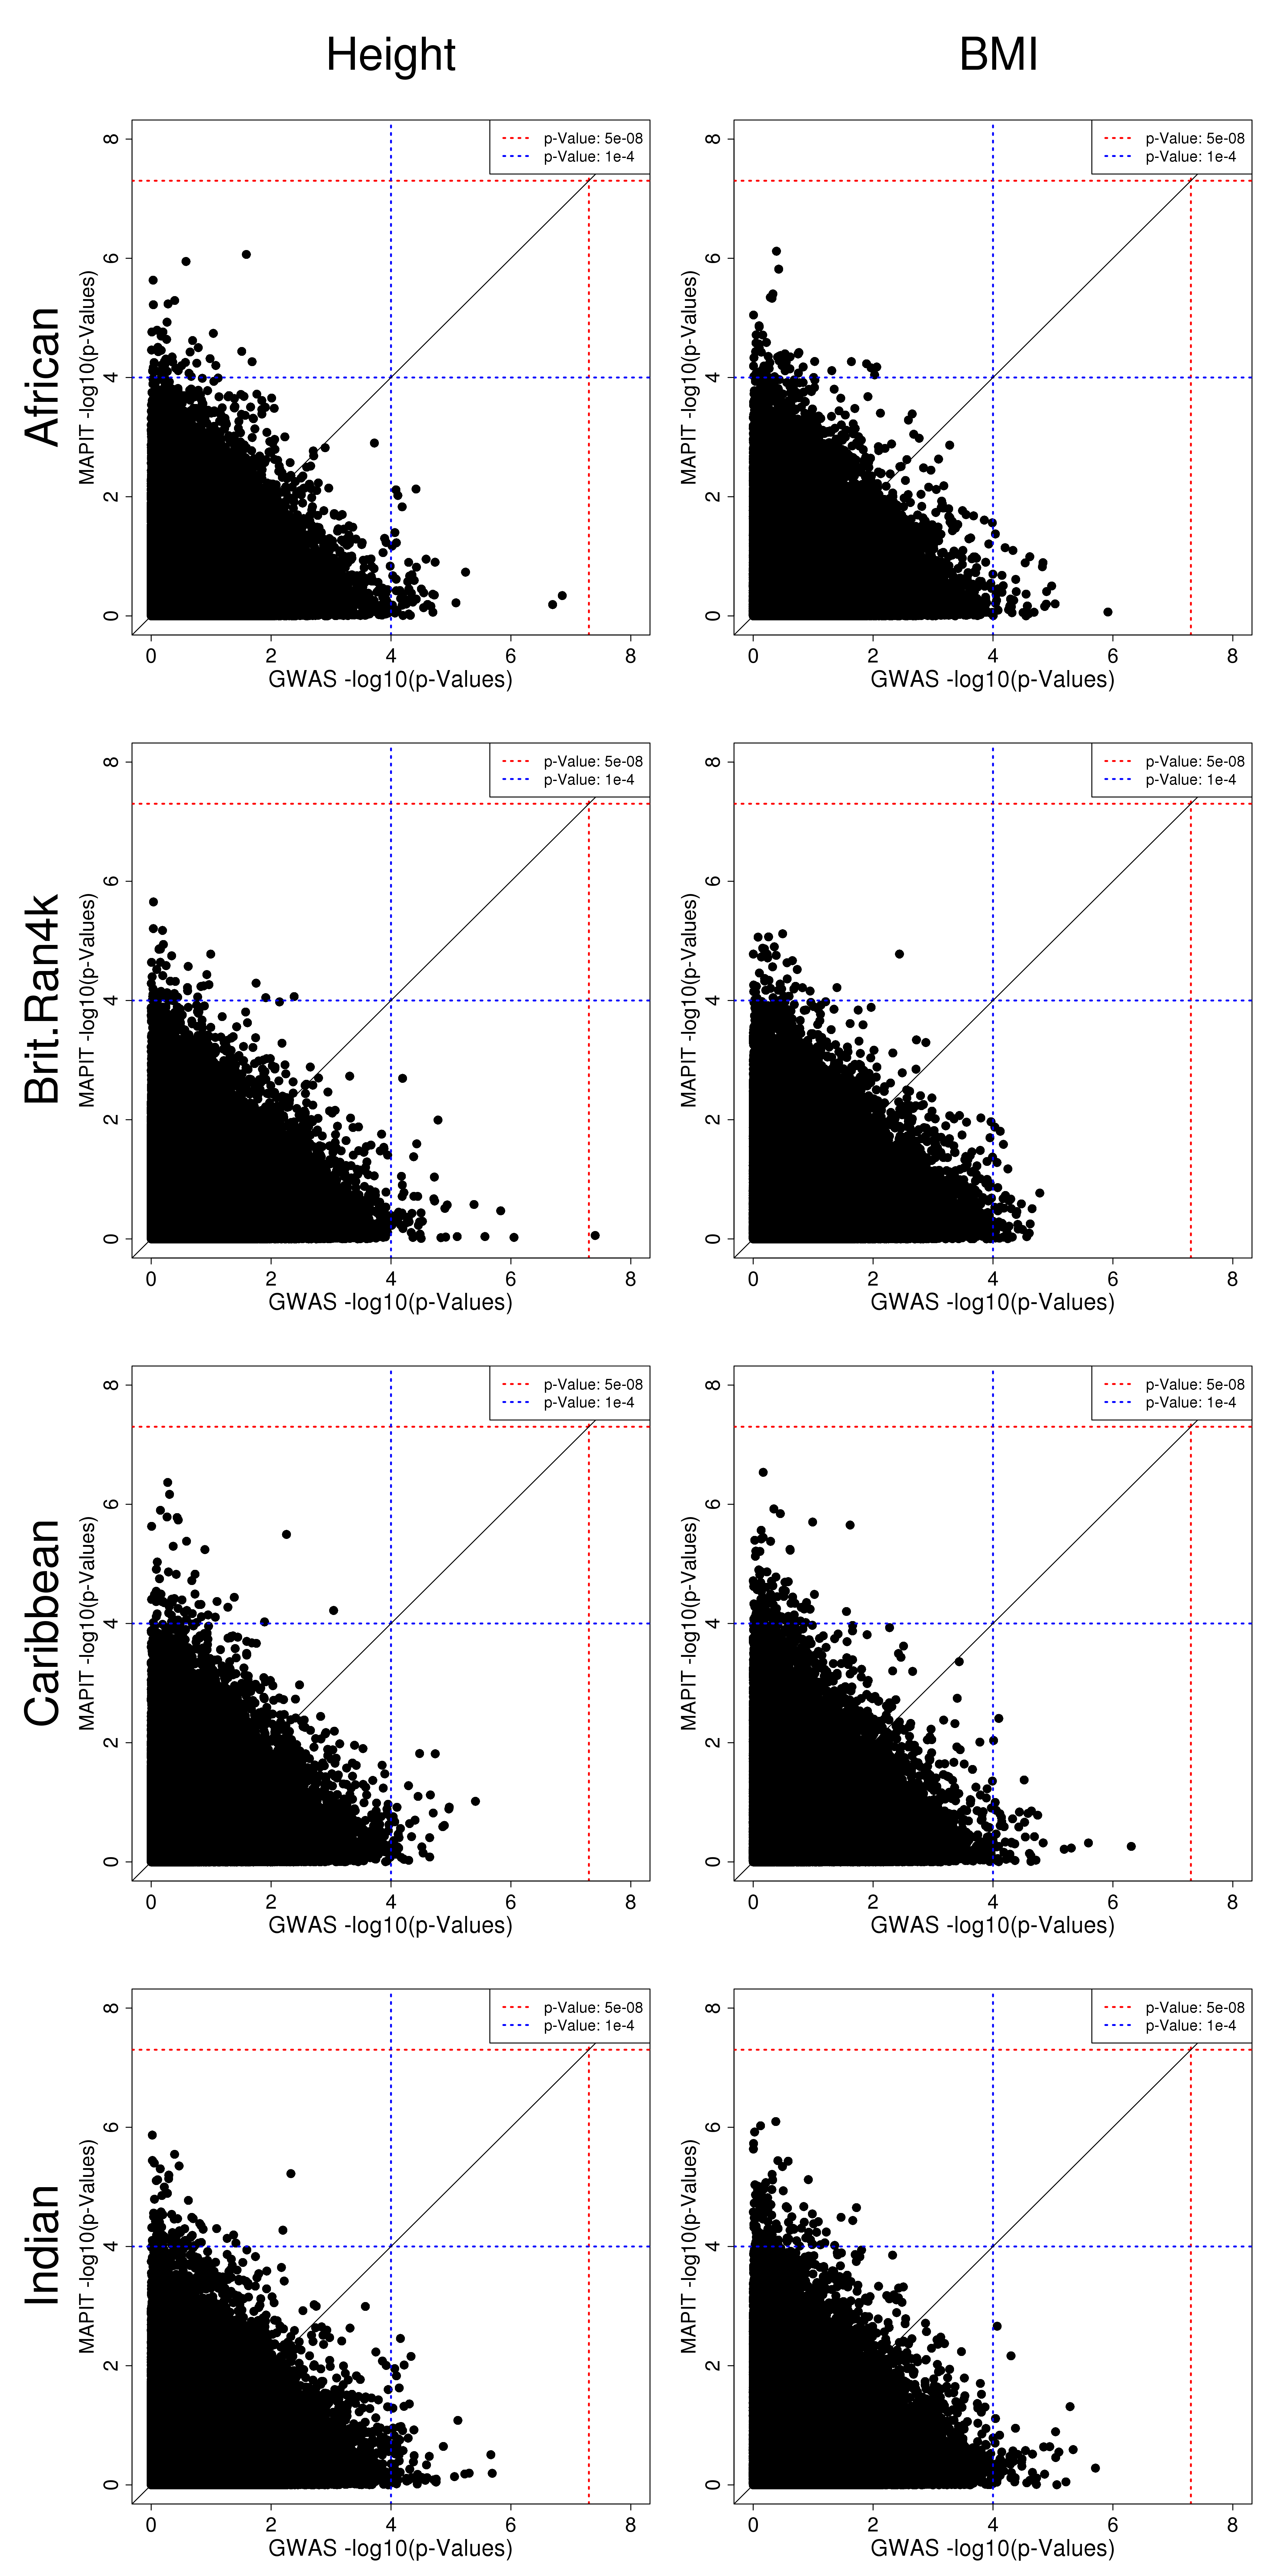
\includegraphics[scale=.3]{Images/Supp/InterPath_Supp_Figure_MAPITvsGWAS_vs2.png}
%\caption[TBD]{\textbf{MAPIT vs. GWAS Results}.}
%\label{InterPath-Supp-Figure-MAPITvsGWAS}
%\end{figure}
%\clearpage

\setlength{\footskip}{3cm}
\begin{figure}[htbp]
\centering
\vspace*{-2cm}
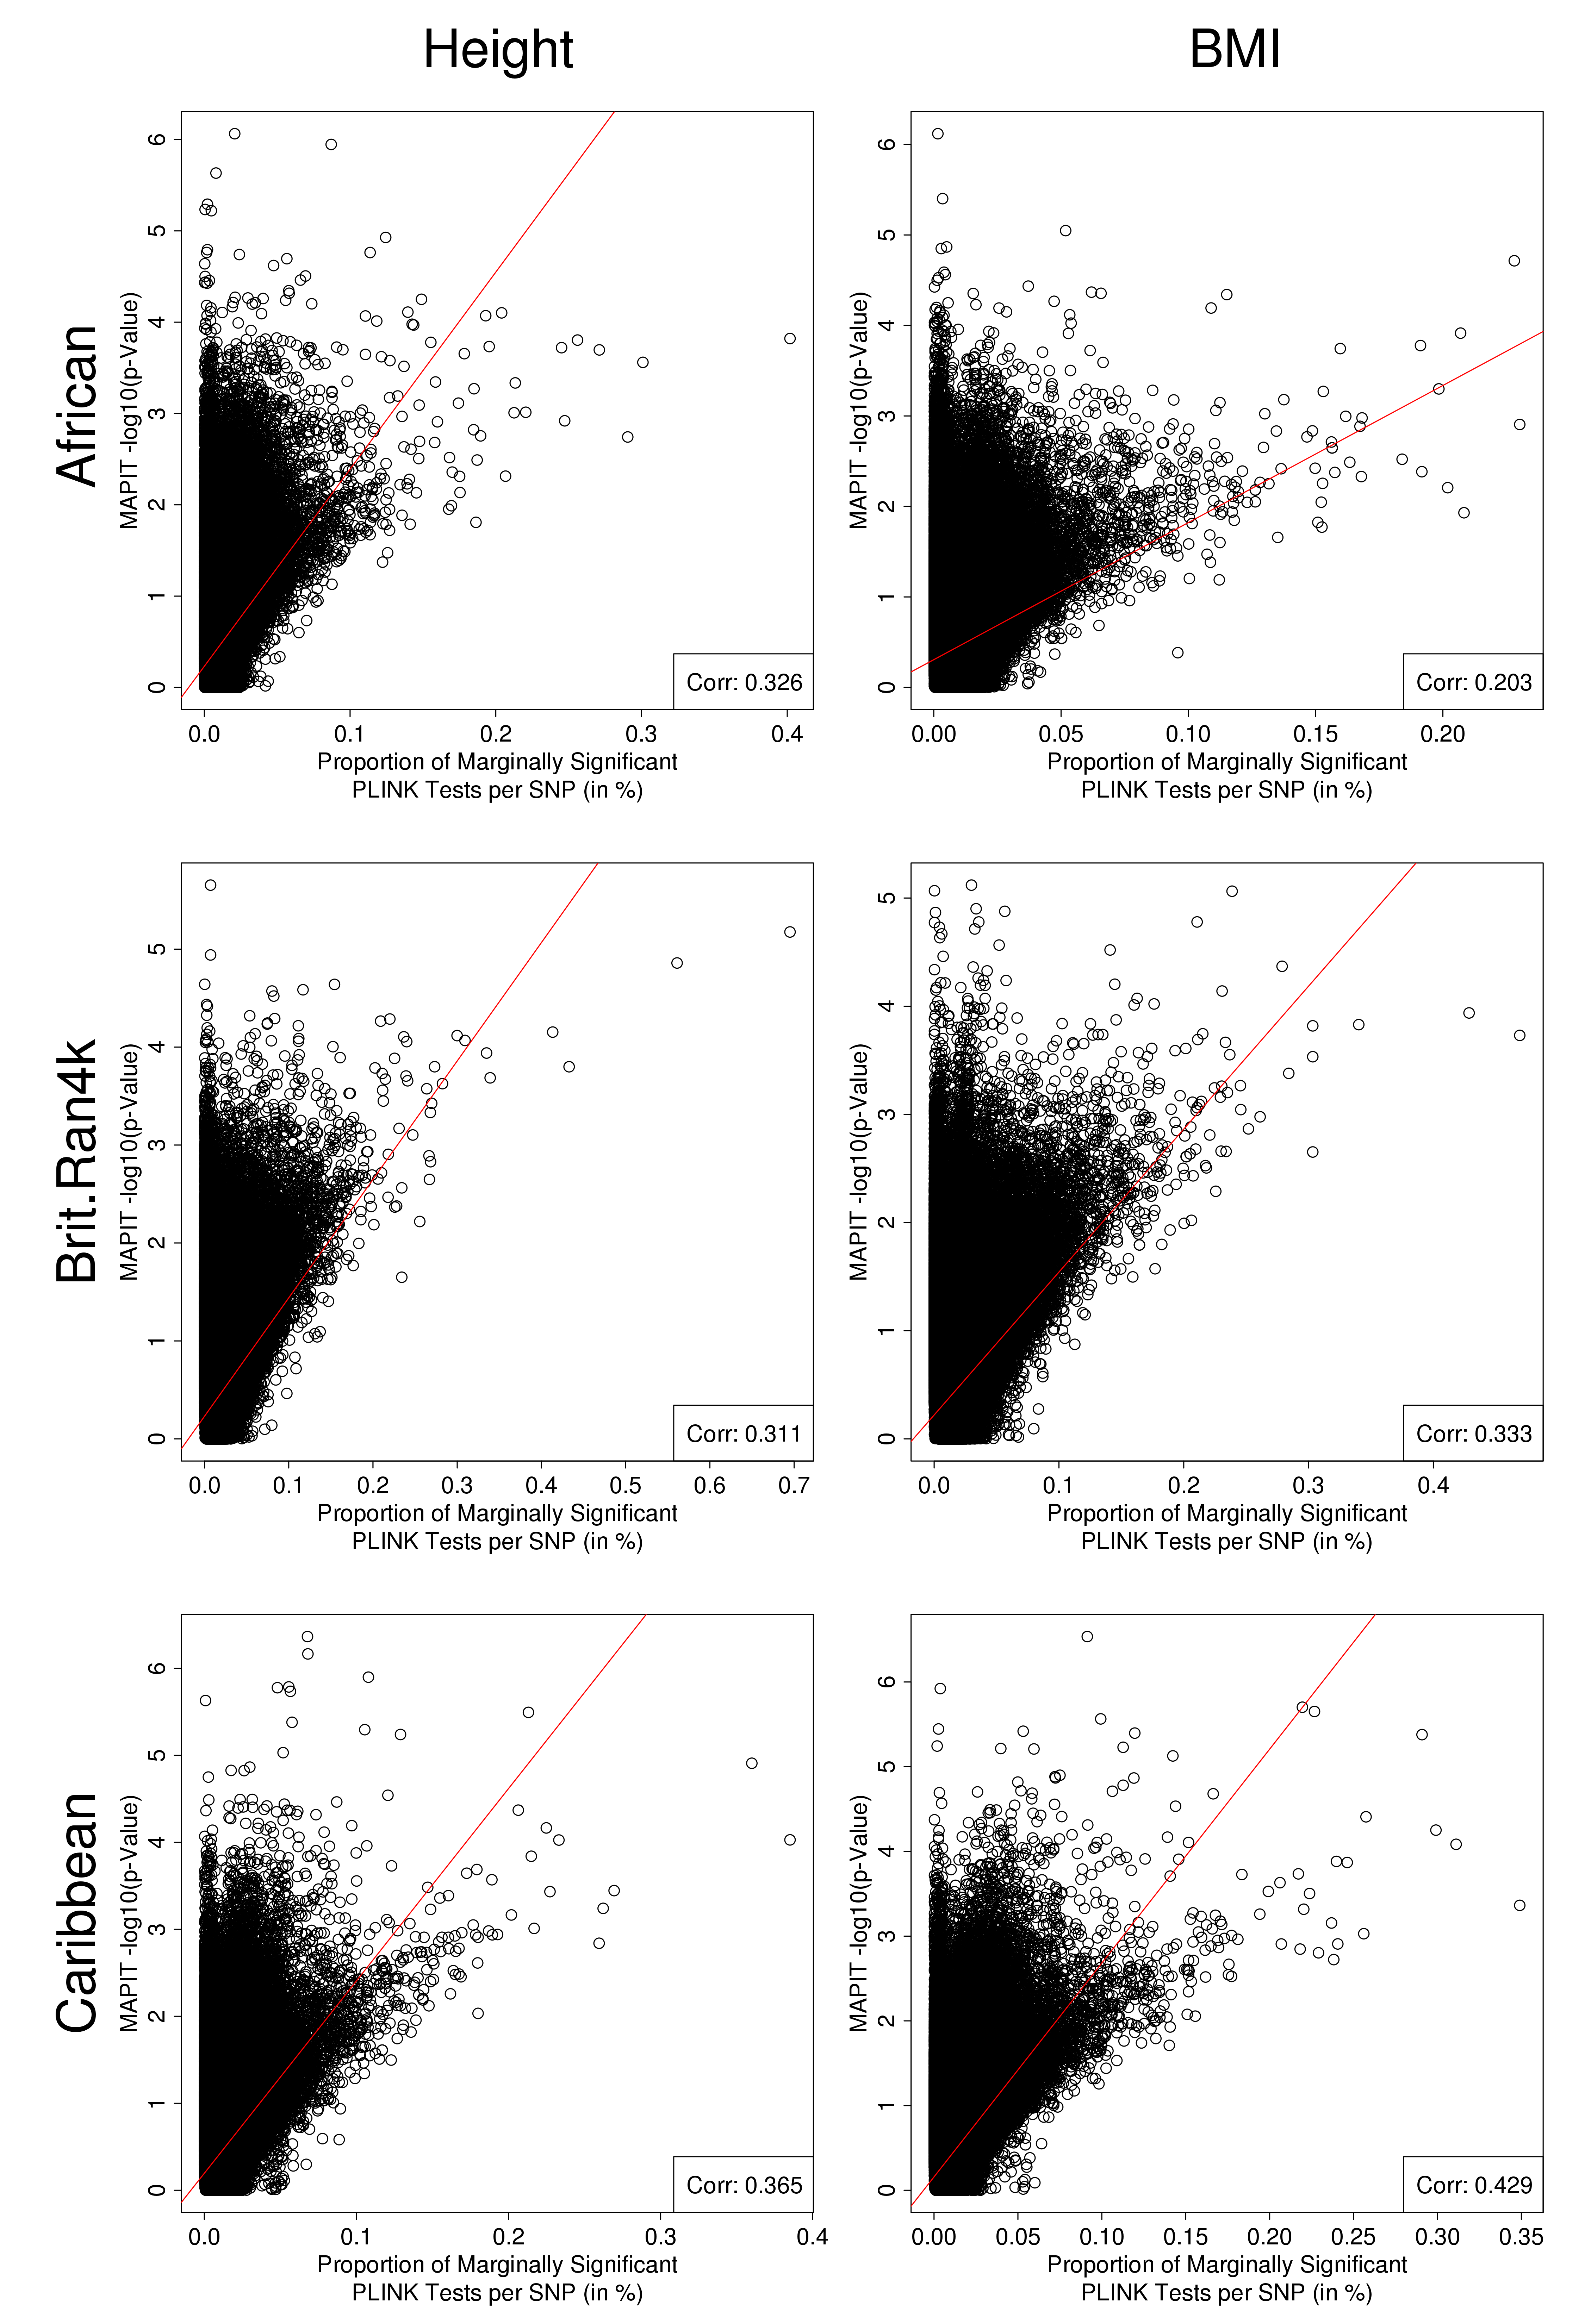
\includegraphics[scale=.3]{Images/Supp/InterPath_Supp_Figure_PLINKvsMAPIT_vs3_AllPops_HeightBMI_pt1.png}
\caption[TBD]{\textbf{Comparison of single-SNP epistasis methods in height and BMI, per subgroup}. Caption continued at end of figures.}
\label{InterPath-Supp-Figure-MAPITvsPLINK-HeightBMI-AllPops-a}
\end{figure}
\clearpage
\setlength{\footskip}{1cm}
\addtocounter{figure}{-1}

\setlength{\footskip}{3cm}
\begin{figure}[htbp]
\centering
\vspace*{-2cm}
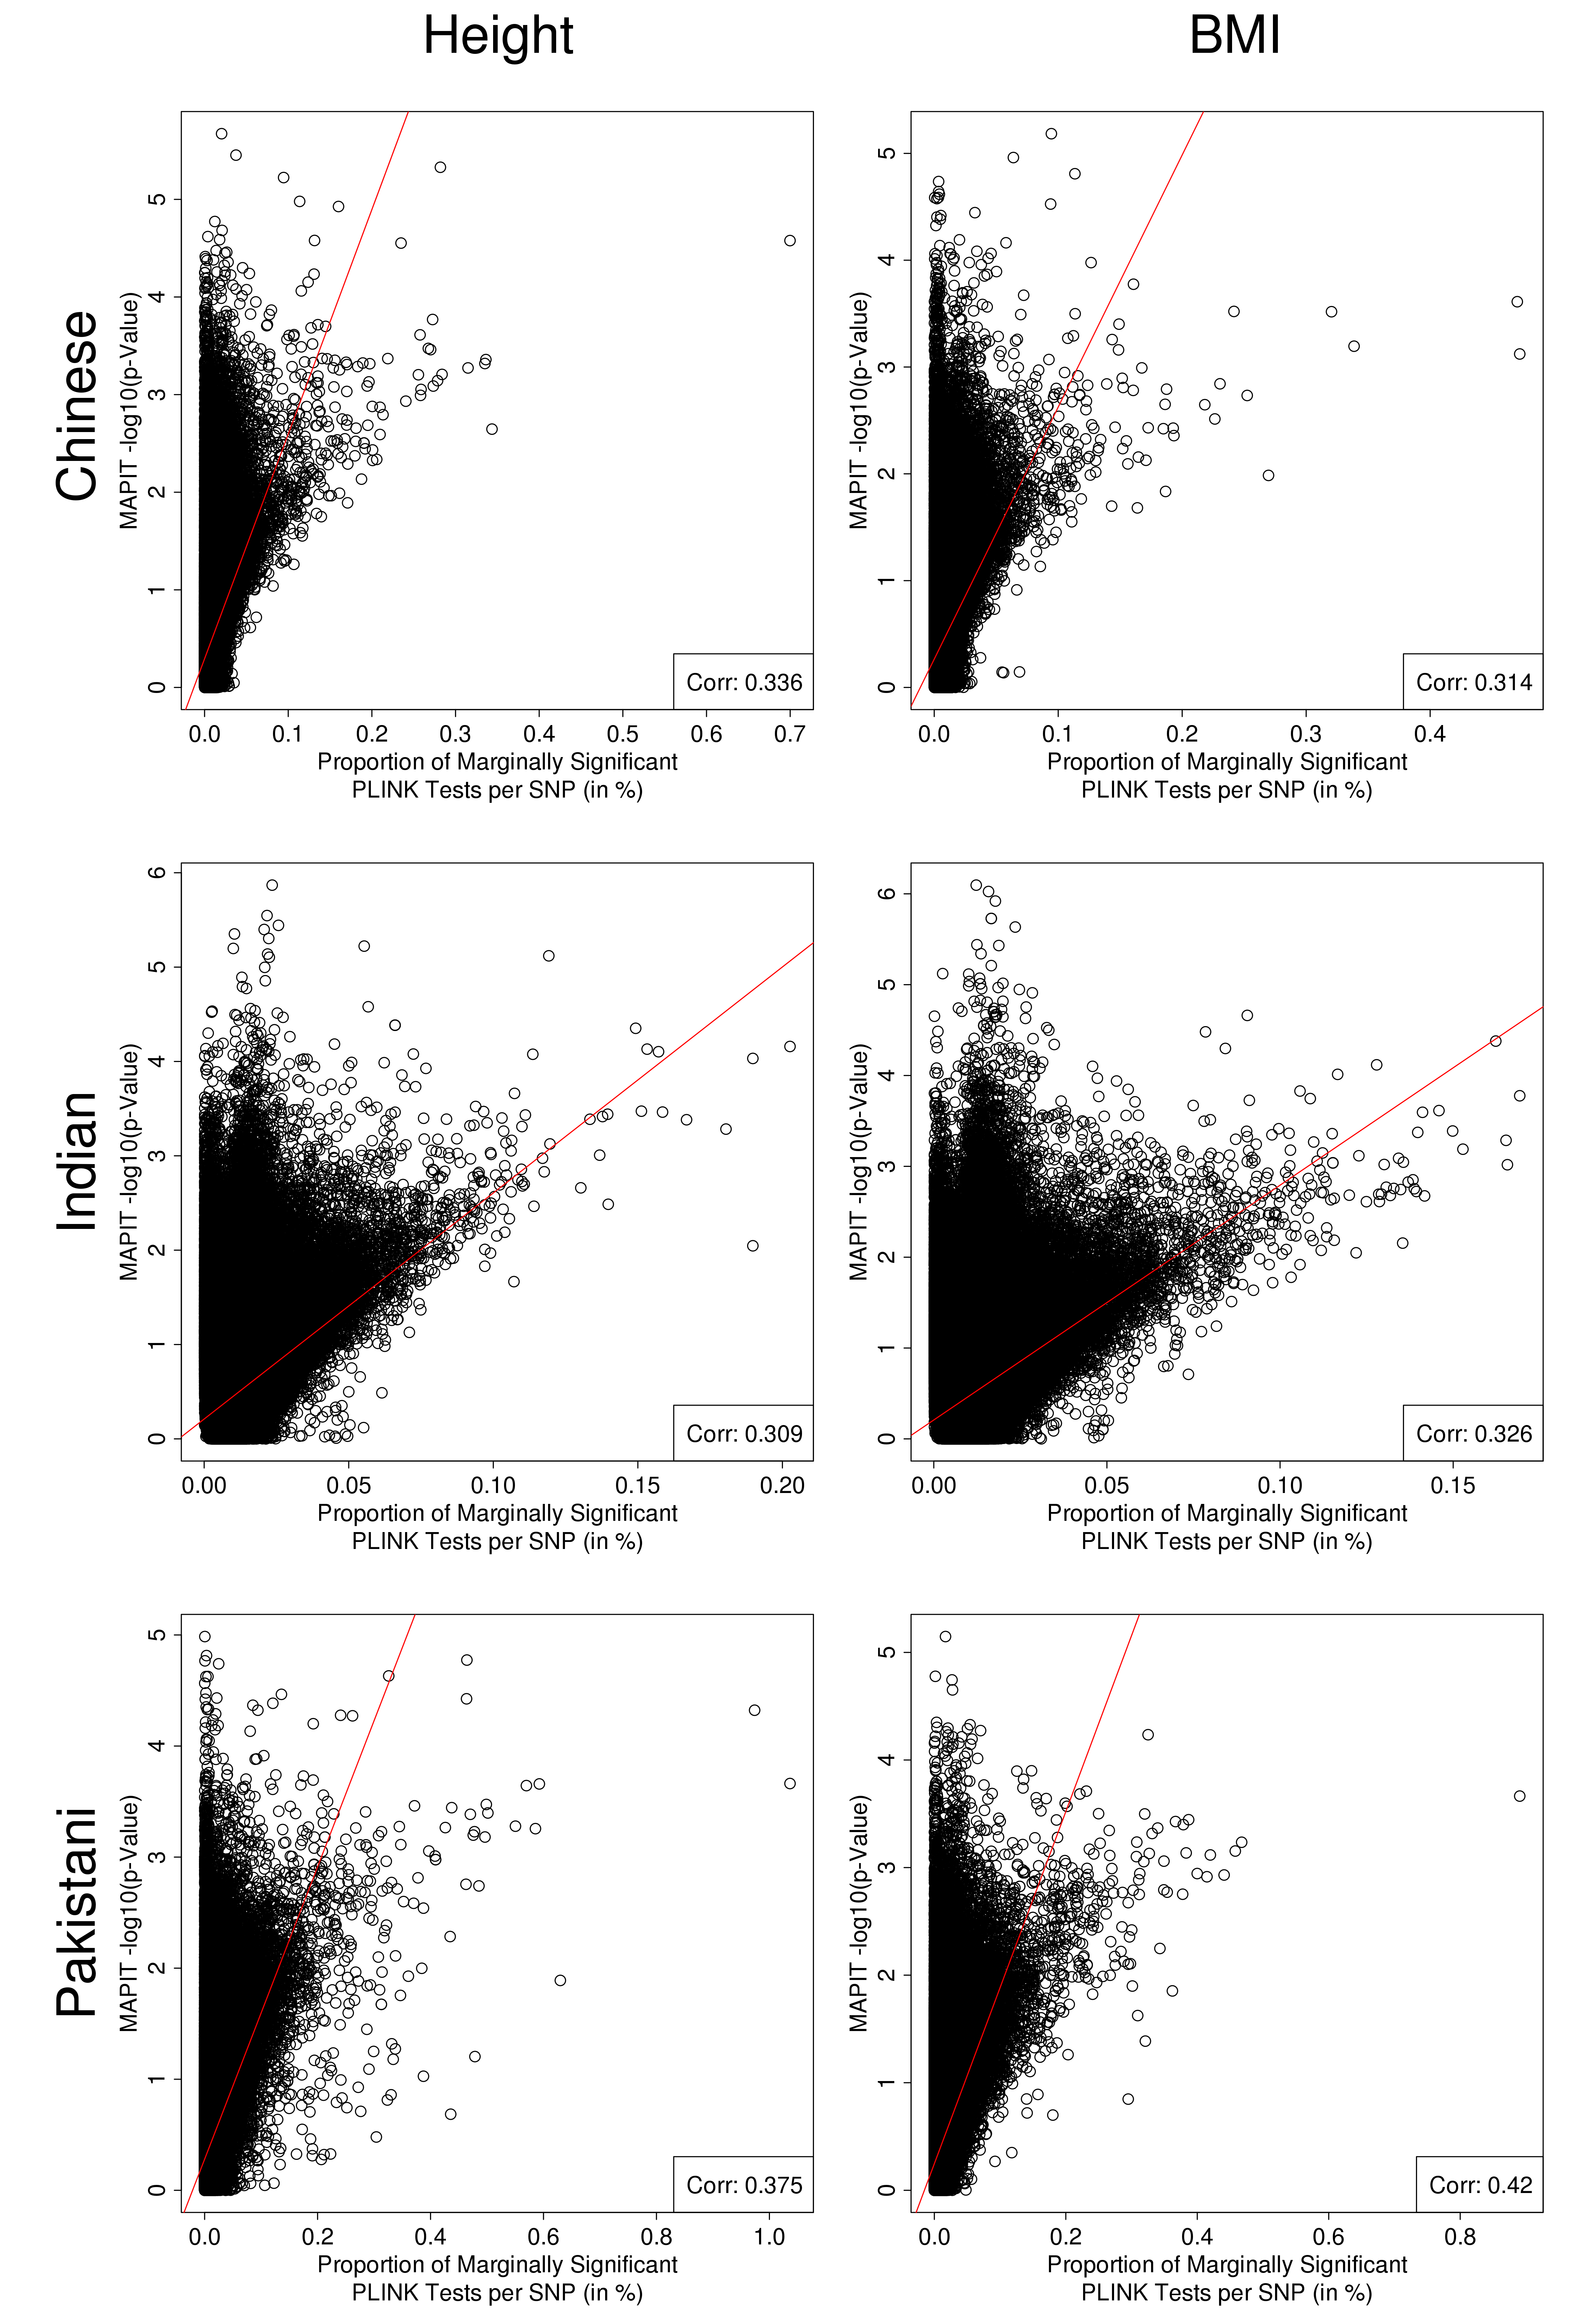
\includegraphics[scale=.3]{Images/Supp/InterPath_Supp_Figure_PLINKvsMAPIT_vs3_AllPops_HeightBMI_pt2.png}
\caption[TBD]{\textbf{Comparison of single-SNP epistasis methods in height and BMI, per subgroup}. Caption continued at end of figure.}
\label{InterPath-Supp-Figure-MAPITvsPLINK-HeightBMI-AllPops-b}
\end{figure}
\clearpage
\setlength{\footskip}{1cm}
\addtocounter{figure}{-1}

\begin{figure} [t!]
\caption[TBD]{\textbf{Comparison of single-SNP epistasis methods in height and BMI, per subgroup}. The figure shows the single-SNP PLINK results vs. MAPIT results for height and BMI in each UKB subgroup. For each individual plot, the PLINK results are shown on the $x$-axis as the proportion of marginally significant interactions per SNP (where marginally significant is defined as $p$-value $< 1\times10^{-4}$) and the MAPIT results are shown on the $y$-axis as the -$\log_{10}$ of the MAPIT $p$-values. The dotted red line shows the line of best fit, and the correlation between the two metrics is shown in the legend. For many of these plots we observe a subset of SNPs with greater marginal epistasis (higher -$\log_{10}$ $p$-values) beginning to correlate with having larger proportions of marginally significant SNP-by-SNP interactions. Seeing the same signal between two different approaches suggests there may be evidence for epistasis on the single-SNP level, albeit weak.}
\label{InterPath-Supp-Figure-MAPITvsPLINK-HeightBMI-All-caption}
\end{figure}
\clearpage

\begin{figure}[htbp]
\centering
\hspace*{-.9cm}
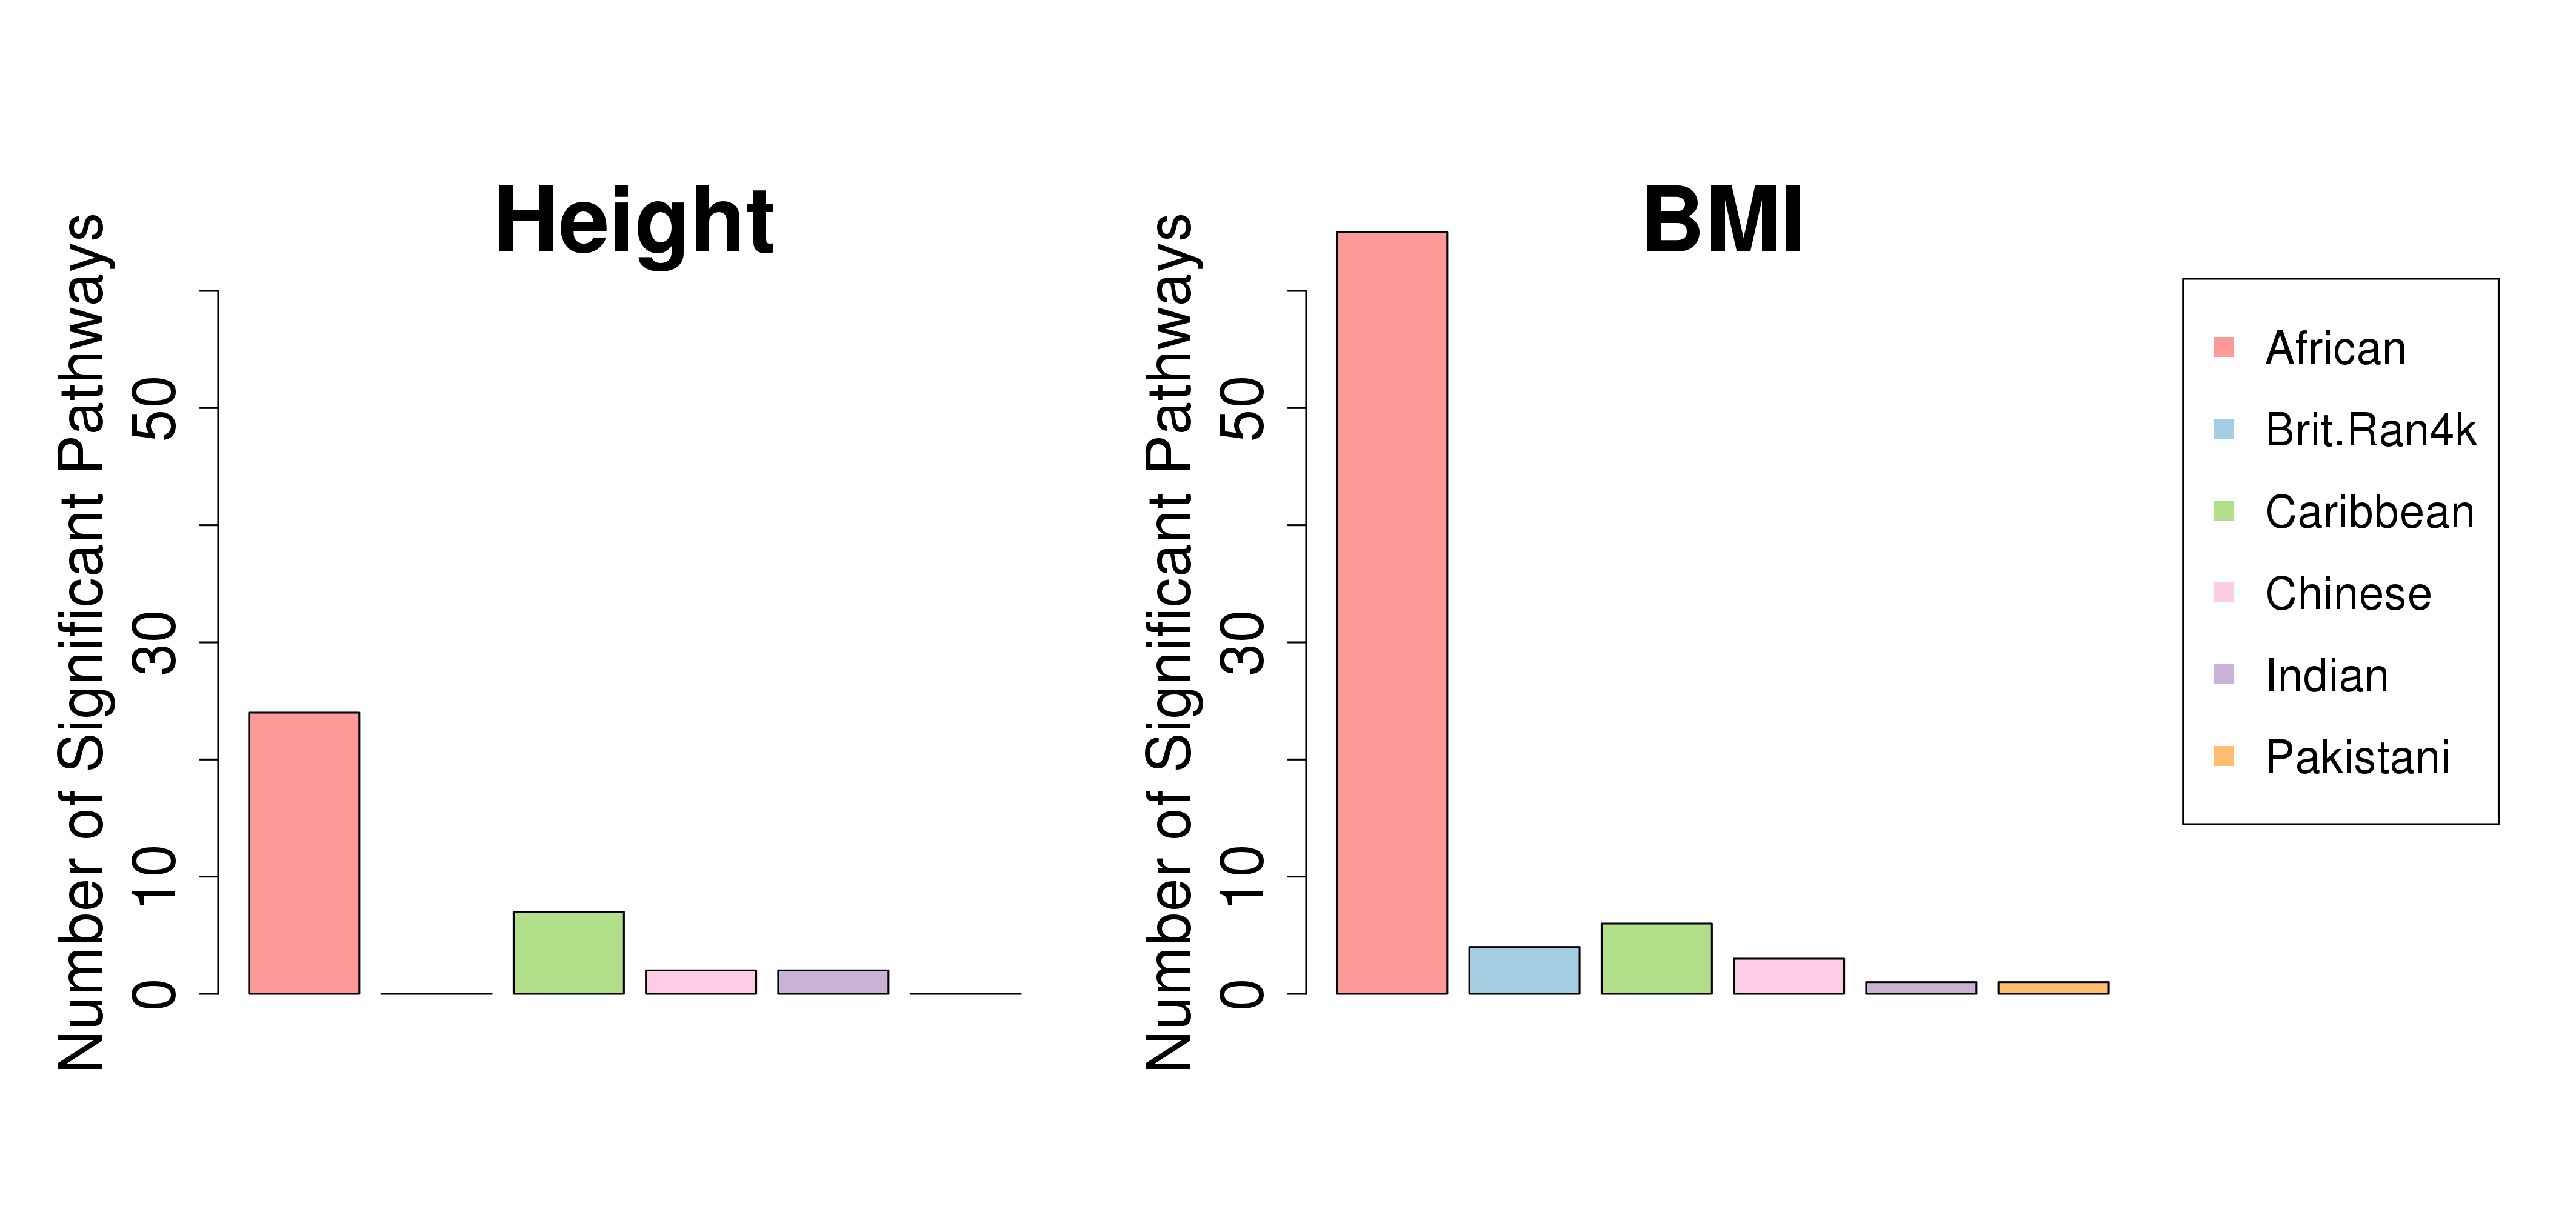
\includegraphics[scale=.45]{Images/Supp/InterPath_Supp_Figure_Barplots_REACTOME_vs2.png}
\caption[TBD]{\textbf{Numbers of REACTOME pathways that have significant marginal epistasis, per subgroup}. The barplots show the number of genome-wide significant pathways found from running MAPIT-R for both height and BMI in the REACTOME database on each of our UKB subgroups. Genome-wide significance was determined by using Bonferroni-corrected $p$-value thresholds based on the number of pathways tested in each phenotype, subgroup, and pathway database combination. As shown in these results, we find across all phenotype and database combinations that the African subgroup has the largest numbers of significant pathways. For lists of the specific significant pathways per subgroup, phenotype, and database combination, see Supplementary Tables \ref{InterPath-Supp-Table-TopPathways-KEGG-Height-a}\textcolor{blue}{-d}.}
\label{InterPath-Supp-Figure-Barplots-REACTOME}
\end{figure}
\clearpage

\begin{figure}[htbp]
\centering
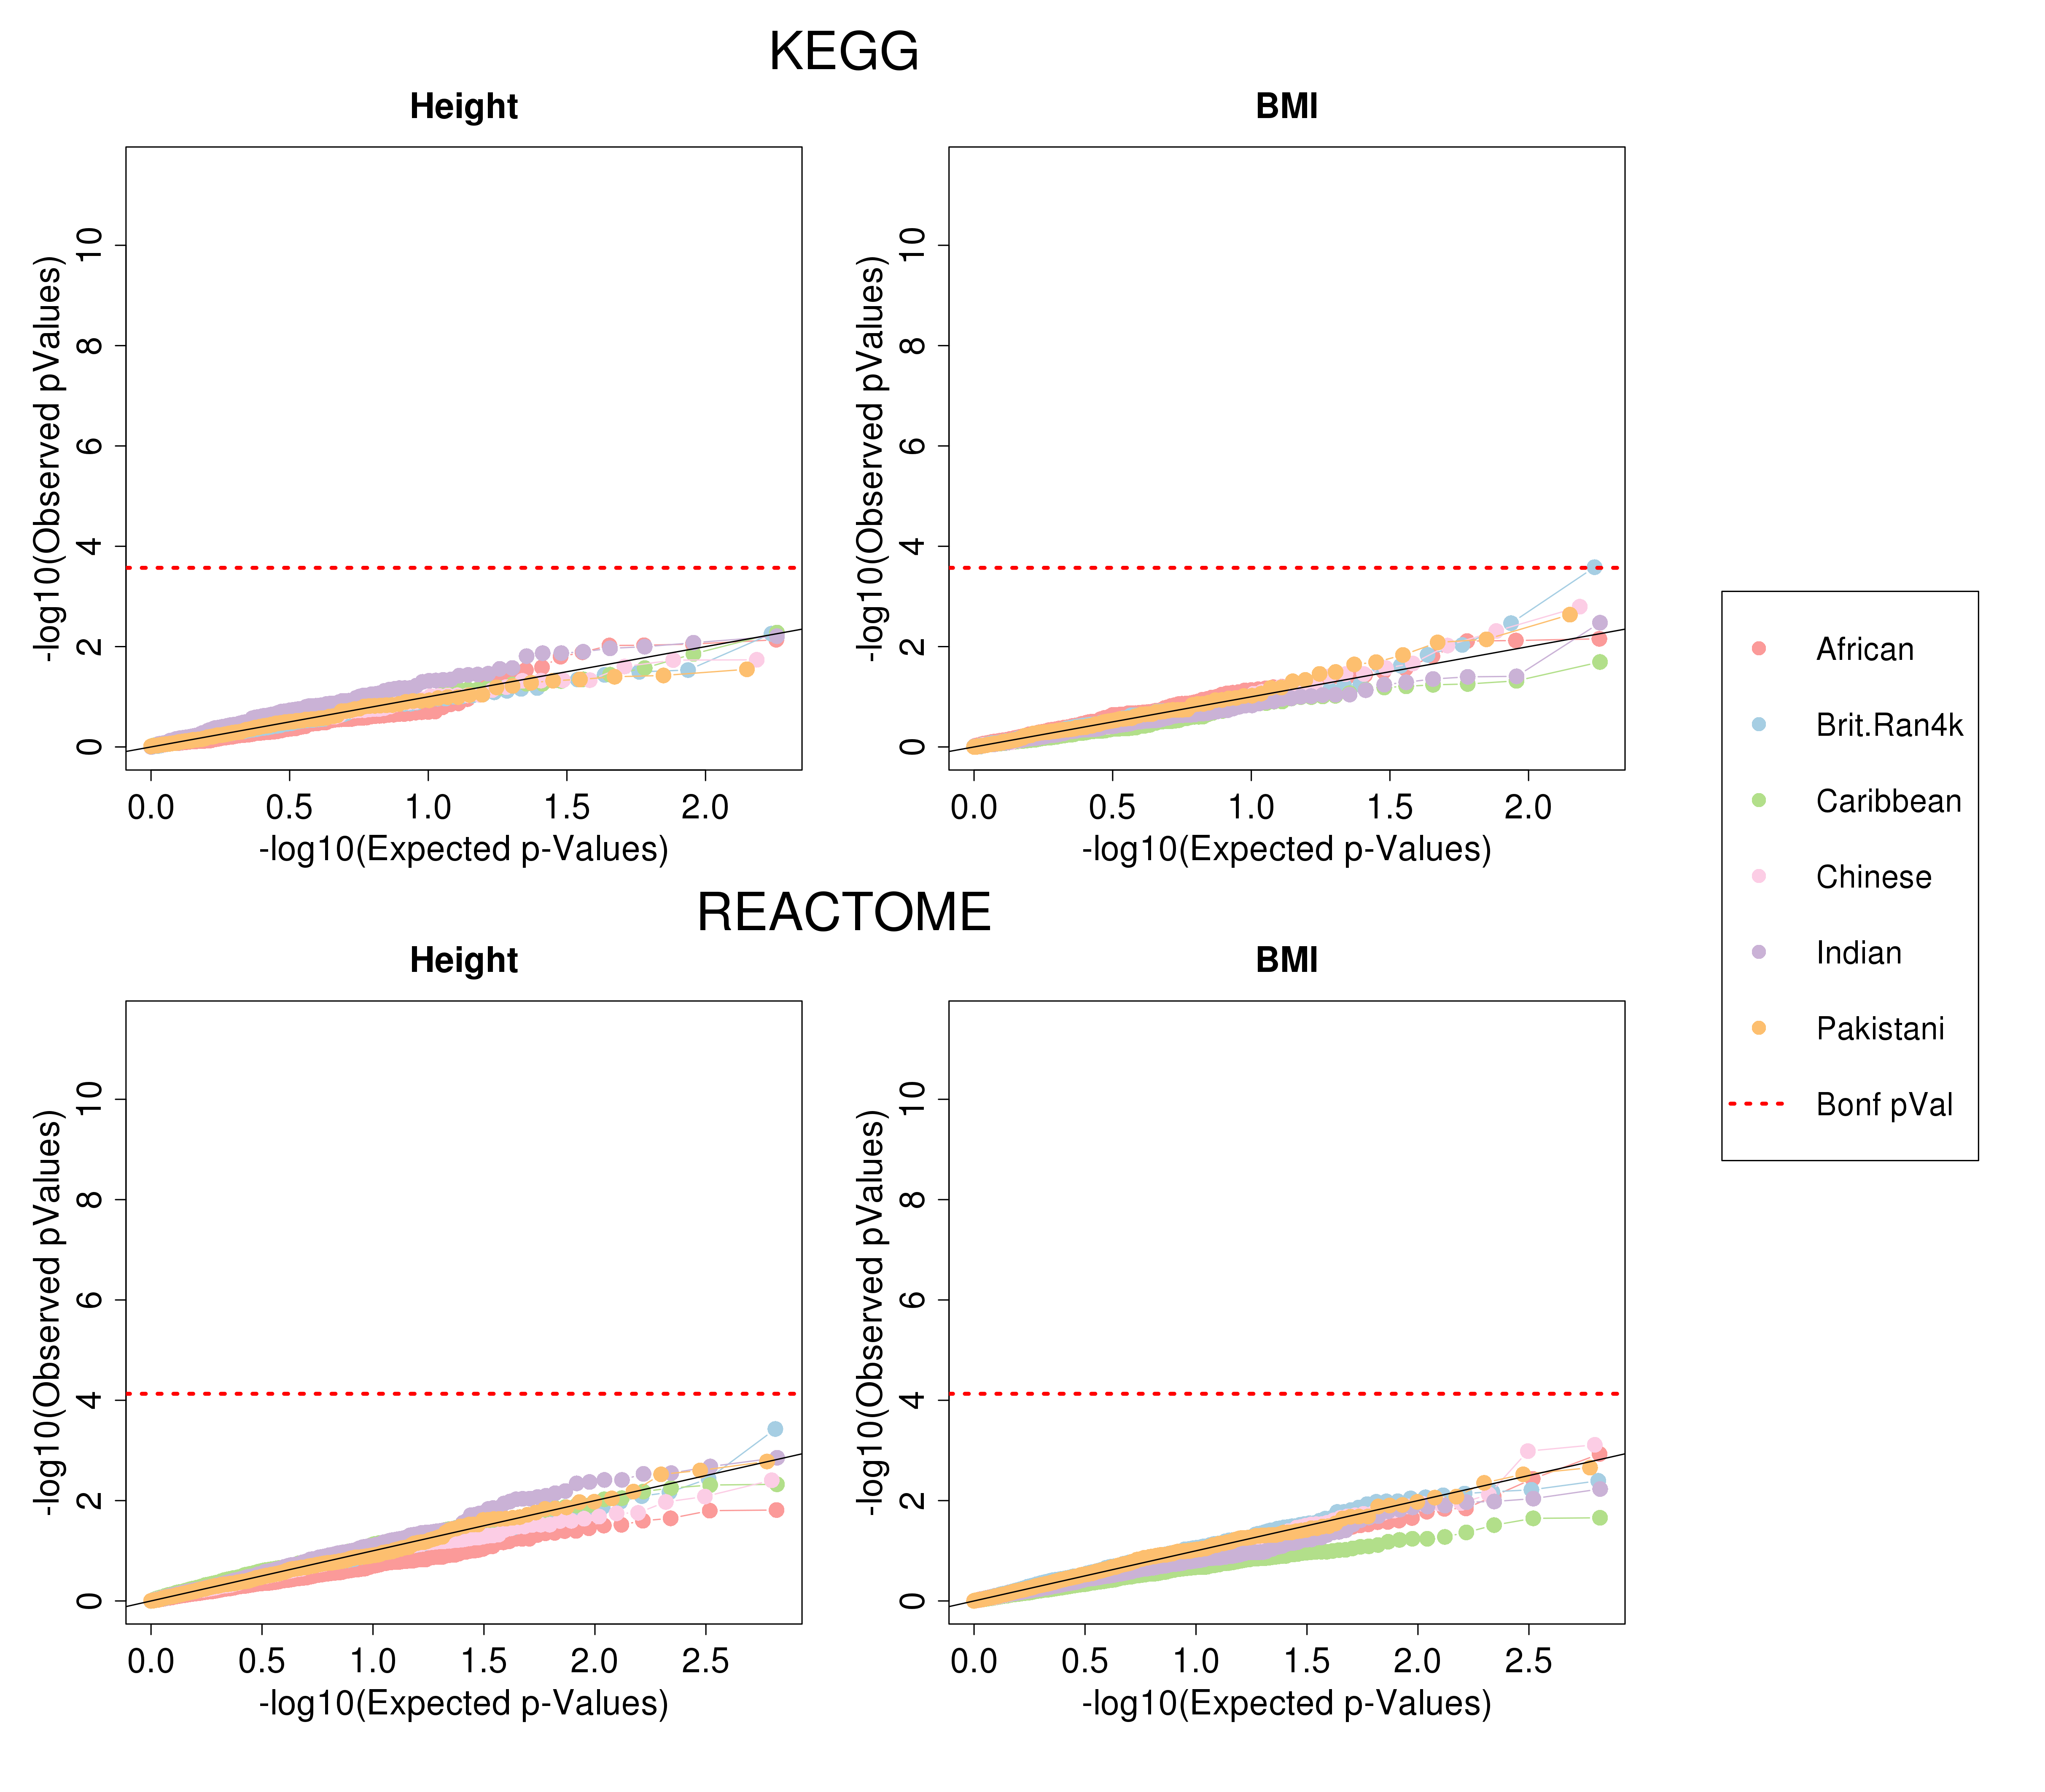
\includegraphics[scale=.35]{Images/Supp/InterPath_Supp_Figure_perm1_QQPlots_AllPaths_vs2.png}
\caption[TBD]{\textbf{QQ-Plots of MAPIT-R results using permuted phenotypes, per subgroup}. The figure shows QQ-plots for running MAPIT-R using single, permuted versions of both height and BMI with the KEGG \& REACTOME databases. Phenotypes were permuted within each population subgroup. Shown on the $x$-axis are the -$\log_{10}$ of the expected $p$-values and the on the $y$-axis are on the -$\log_{10}$ of the observed $p$-values. The dotted red line is our Bonferroni-corrected $p$-value threshold based on the number of pathways tested per phenotype and pathway database combination. We find across all UKB subgroup, phenotype, and pathway database combinations that MAPIT-R displays null behavior within the range expected when using permuted phenotypes.}
\label{InterPath-Supp-Figure-perm1-QQPlots-AllPaths}
\end{figure}
\clearpage

\setlength{\footskip}{3cm}
\begin{figure}[htbp]
\centering
\vspace*{-2cm}
\includegraphics[scale=.2]{Images/Supp/InterPath_Supp_Figure_pValHists_vs3.png}
\caption[TBD]{\textbf{$p$-Value histograms of MAPIT-R results using permuted phenotypes, per subgroup}. The figure shows histograms of MAPIT-R $p$-values collected across ten independent phenotype permutation runs for each UKB subgroup. The same phenotype permutation for a given subgroup was used across both pathway databases (i.e. 10 permutations were done for height and 10 done for BMI for each subgroup). Covariates used from the original MAPIT-R analysis were kept the same.}
\label{InterPath-Supp-Figure-10perms-pValHists}
\end{figure}
\clearpage
\setlength{\footskip}{1cm}

\setlength{\footskip}{3cm}
\begin{figure}[htbp]
\centering
\vspace*{-2cm}
\includegraphics[scale=.2]{Images/Supp/InterPath_Supp_Figure_pValsVsNumSNPs_vs2.png}
\caption[TBD]{\textbf{Number of SNPs in a pathway versus a pathway's MAPIT-R $p$-value}. Caption continued on next page.}
\label{InterPath-Supp-Figure-pValsVsNumSNPs}
\end{figure}
\clearpage
\setlength{\footskip}{1cm}

\addtocounter{figure}{-1}
\begin{figure} [t!]
  \caption{\textbf{Number of SNPs in a pathway versus a pathway's MAPIT-R $p$-value}. The figure shows plots comparing the MAPIT-R $p$-values from our main analysis to the number of SNPs present in each pathway. Results for every UKB subgroup, phenotype, and pathway database combinations are shown. The dotted red line is the line of best fit and the legend provides the regression coefficient and its associated $p$-value. We observe that for most combinations there is a significant relationship between MAPIT-R $p$-value and the number of SNPs present in a pathway. This follows our hypothesis that combining SNPs together in a joint analysis might provide greater power to detect marginal epistasis than analyzing each SNP independently. We note, however, that these results appear to not solely be driven just by the presence or absence of large SNP counts -- conducting this same analysis on one of our sets of permuted phenotypes we now find very few significant relationships between MAPIT-R $p$-values and pathway SNP counts (Supplementary Figure \ref{InterPath-Supp-Figure-pValsVsNumSNPs-perm1}).}
\label{InterPath-Supp-Figure-pValsVsNumSNPs-Caption}
\end{figure}
\clearpage

\setlength{\footskip}{3cm}
\begin{figure}[htbp]
\centering
\vspace*{-2cm}
\includegraphics[scale=.2]{Images/Supp/InterPath_Supp_Figure_pValsVsNumSNPs_perm1_vs2.png}
\caption[TBD]{\textbf{Number of SNPs in a pathway versus a pathway's MAPIT-R $p$-value using permuted phenotypes}. Caption continued on next page.}
\label{InterPath-Supp-Figure-pValsVsNumSNPs-perm1}
\end{figure}
\clearpage
\setlength{\footskip}{1cm}

\addtocounter{figure}{-1}
\begin{figure} [t!]
  \caption{\textbf{Number of SNPs in a pathway versus a pathway's MAPIT-R $p$-value using permuted phenotypes}. The figure shows plots comparing the MAPIT-R $p$-values from our main analysis to the number of SNPs present in each pathway. For this analysis a single set of our permuted phenotypes (i.e. Supplementary Figure \ref{InterPath-Supp-Figure-perm1-QQPlots-AllPaths}) was used for each UKB subgroup. Results for every subgroup, permuted phenotype, and pathway database combinations are shown. The dotted red line is the line of best fit and the legend provides the regression coefficient and its associated $p$-value. We observe that for very few combinations there is any relationship between MAPIT-R $p$-value and the number of SNPs present in a pathway. For the same analysis on the original set of observed phenotypes, see Supplementary Figure \ref{InterPath-Supp-Figure-pValsVsNumSNPs}.}
\label{InterPath-Supp-Figure-pValsVsNumSNPs-perm1-Caption}
\end{figure}
\clearpage

%\begin{figure}[htbp]
%\centering
%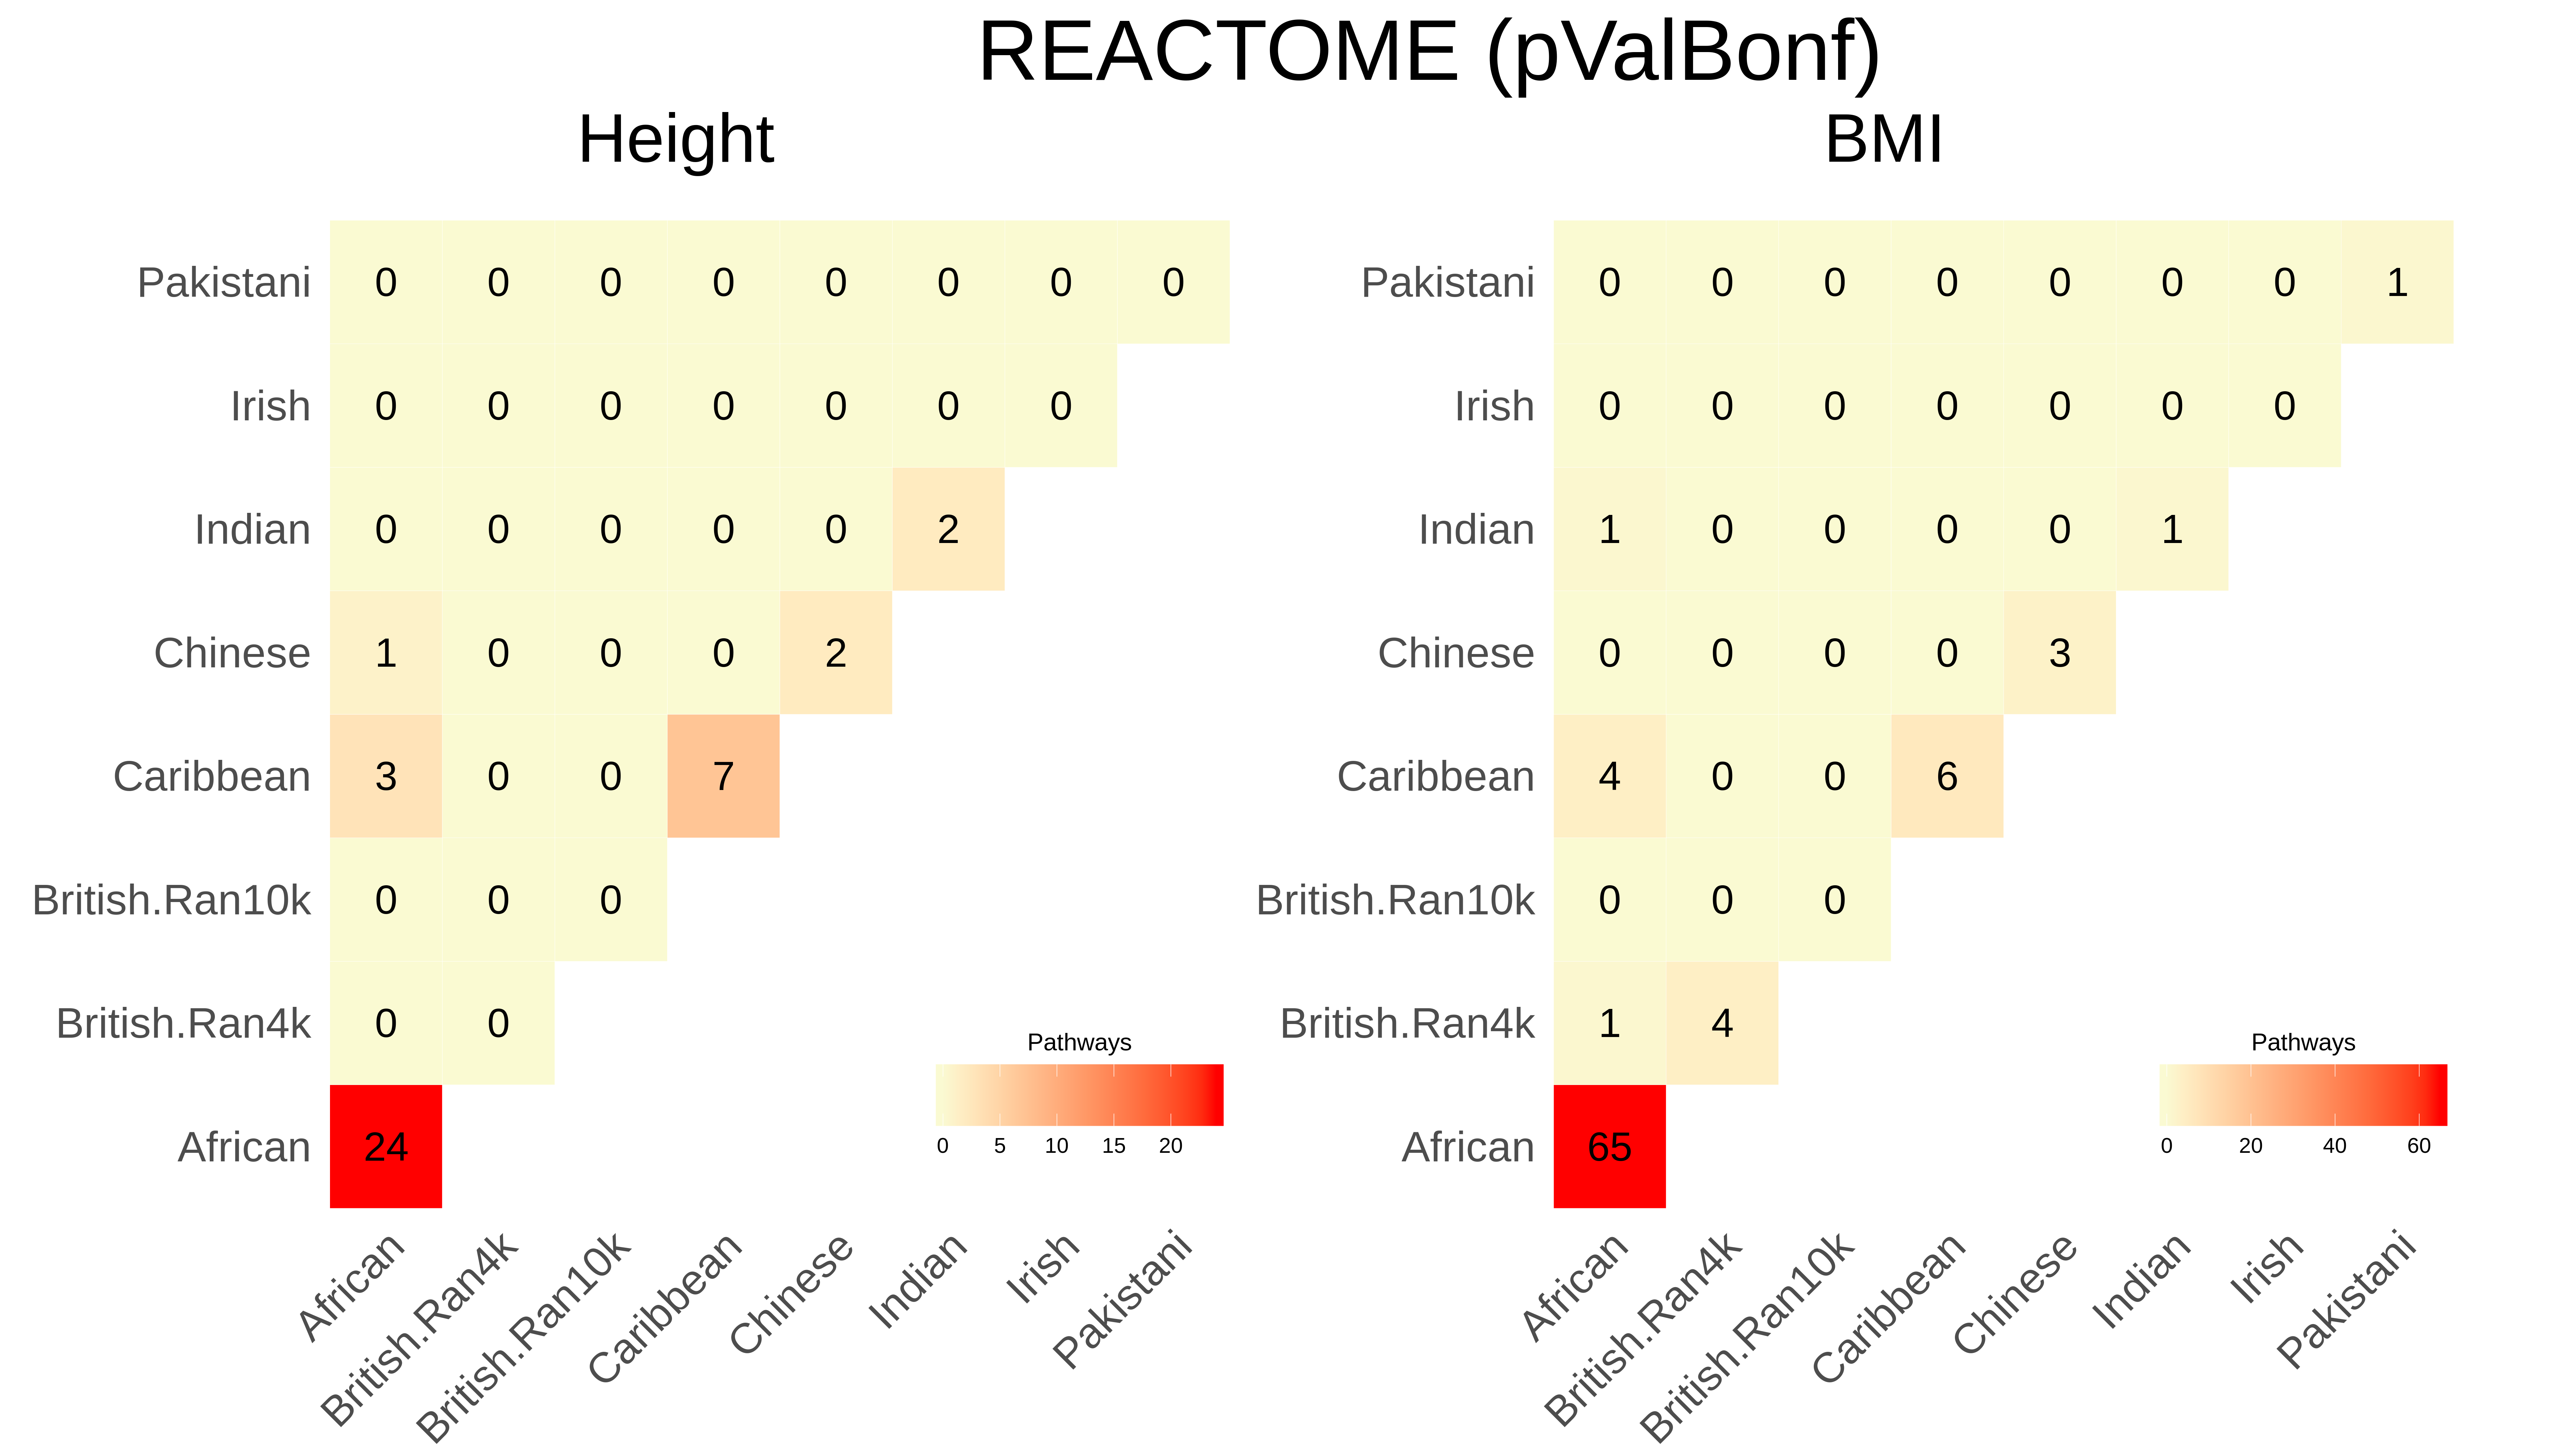
\includegraphics[scale=.225]{Images/Supp/InterPath_Supp_Figure_Heatplots_REACTOME_vs1.png}
%\caption[TBD]{\textbf{TBD}. \\ See above (this would be a supplementary figure).}
%\label{InterPath-Supp-Figure-Heatplots-REACTOME}
%\end{figure}
%\clearpage

\setlength{\footskip}{1cm}
\begin{figure}[htbp]
\centering
\vspace*{-2cm}
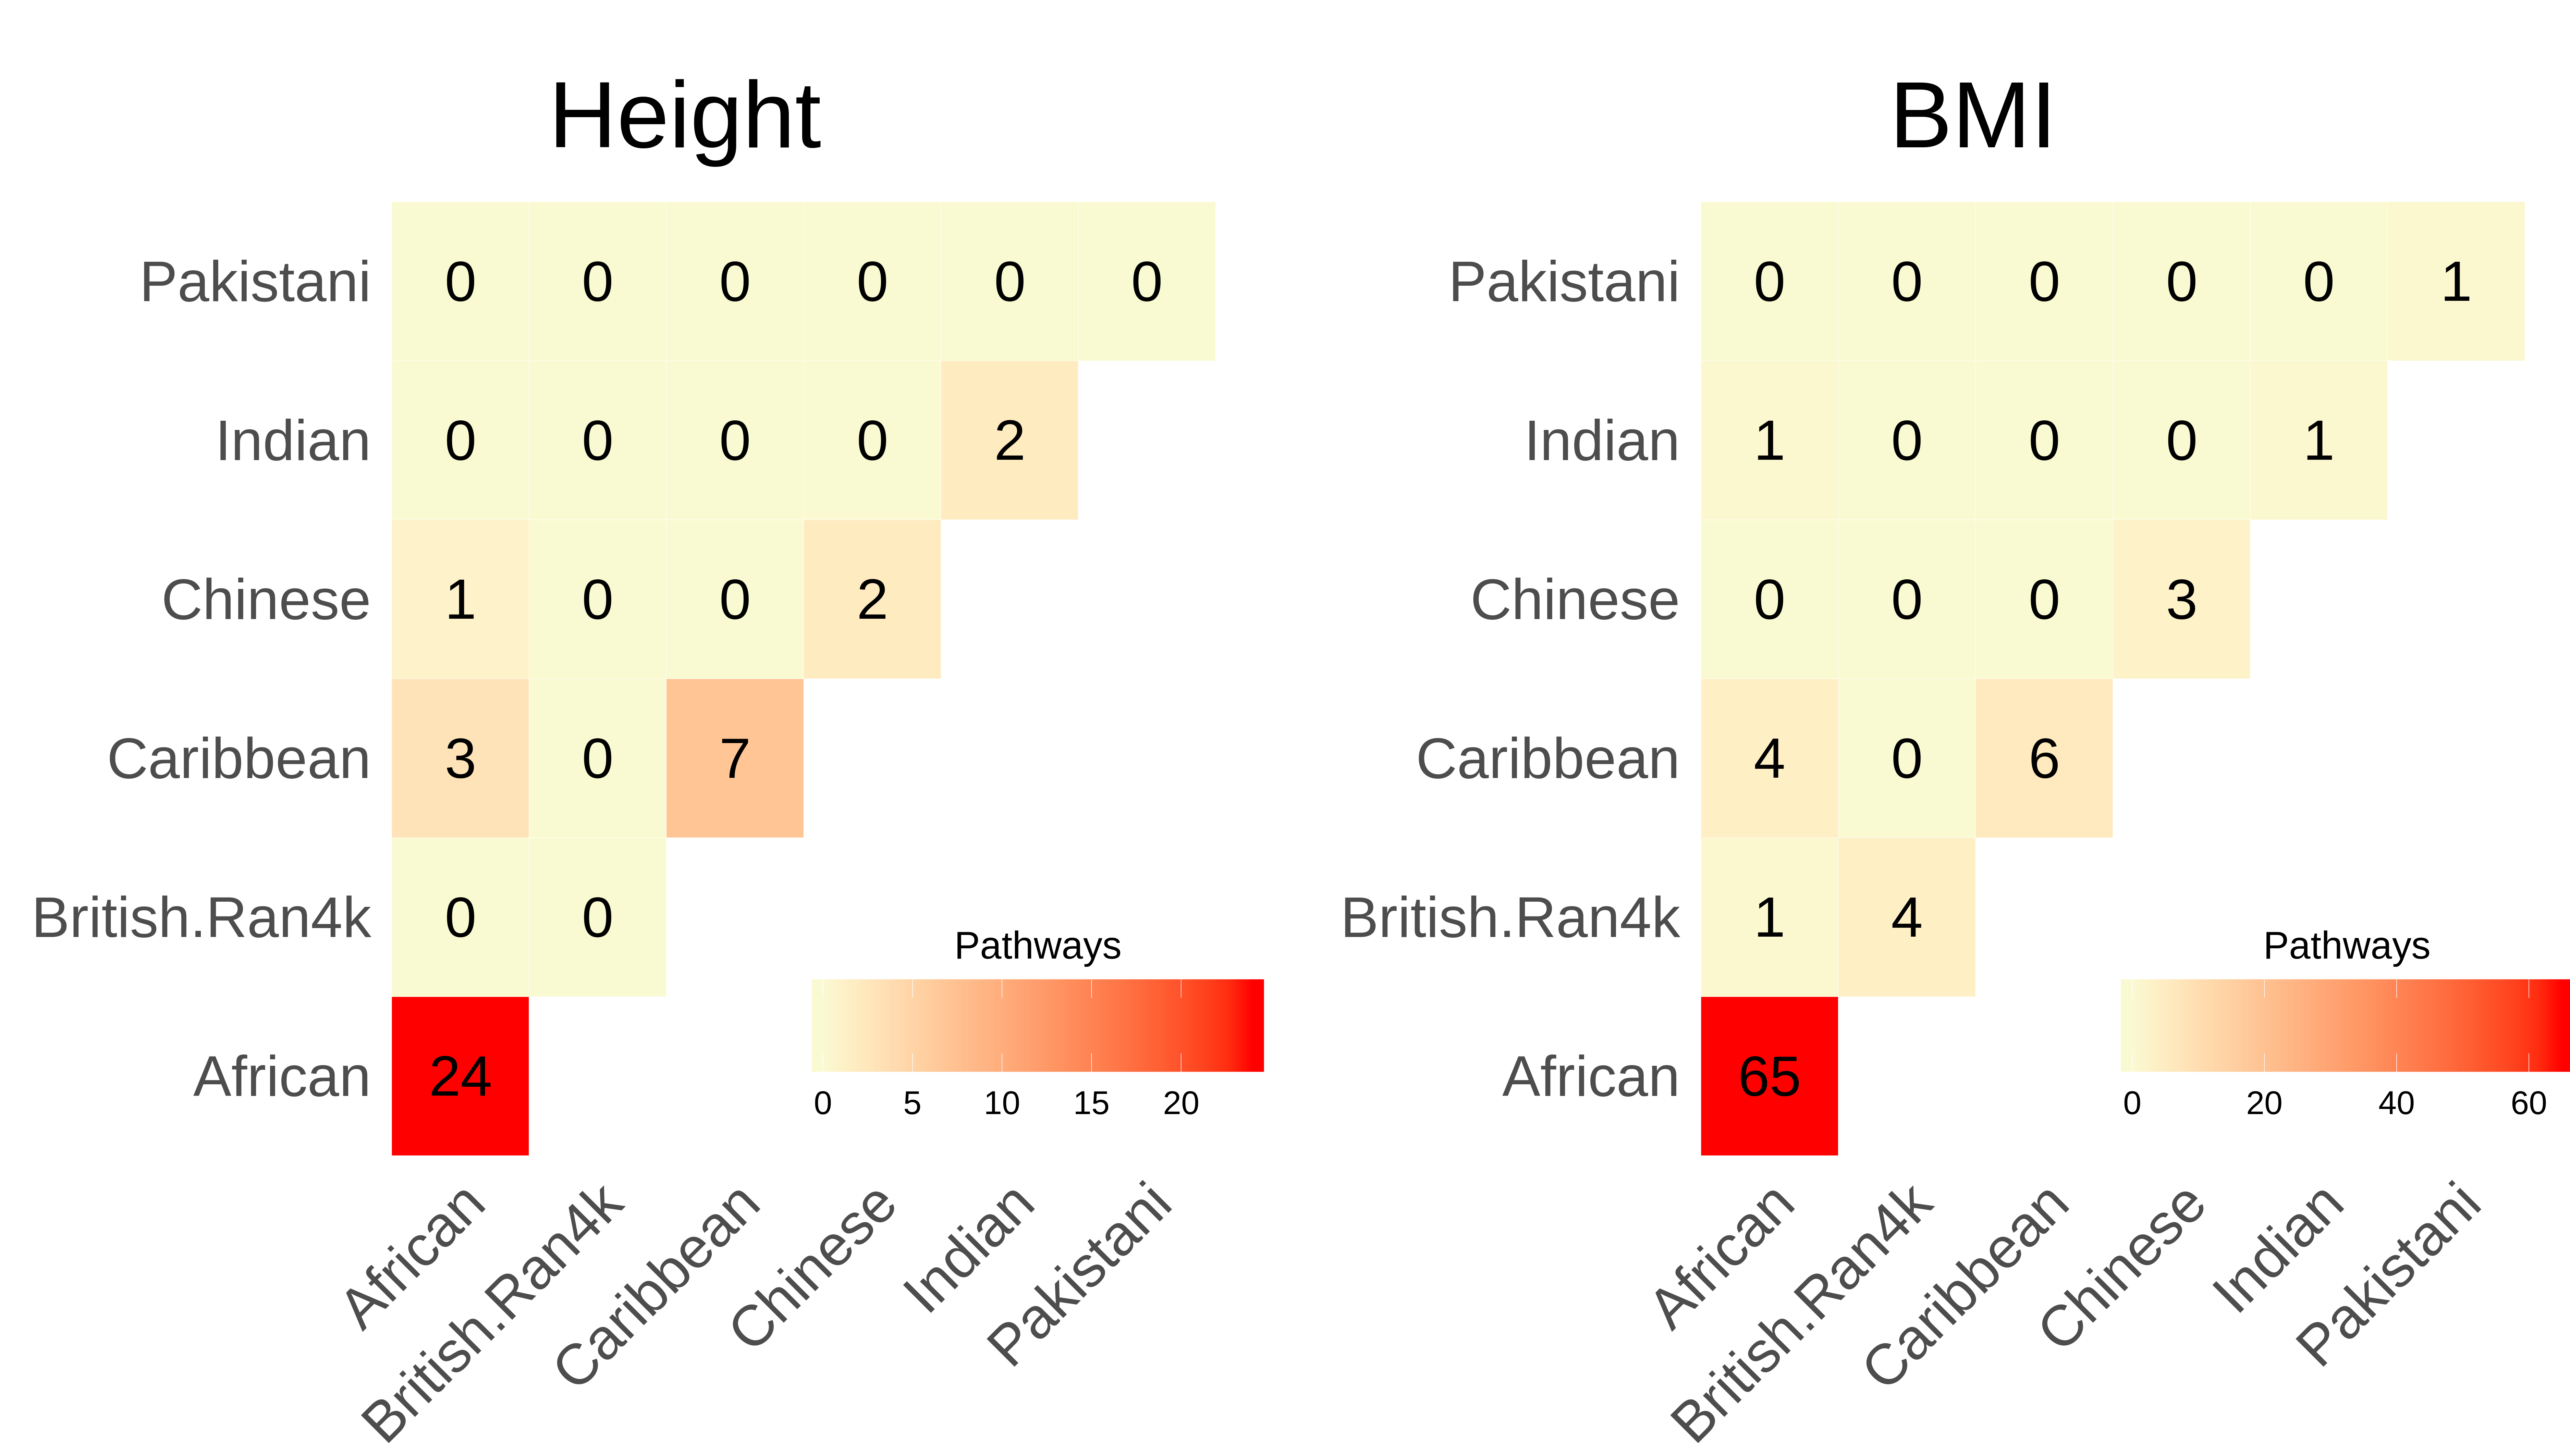
\includegraphics[scale=.225]{Images/Supp/InterPath_Supp_Figure_Heatplots_REACTOME_vs3.png}
\caption[TBD]{\textbf{Overlap of genome-wide significant MAPIT-R pathways between UKB population subgroups: REACTOME}. The heatplots show the numbers of genome-wide significant MAPIT-R pathways that overlap between each UKB subgroup for height and BMI in the REACTOME database. The diagonal shows the total number of genome-wide significant pathways per population subgroup. We observe that most subgroups often have overlap with the African subgroup but rarely do so with the remaining non-African subgroups. For results from the KEGG database see Figure \ref{InterPath-Main-Figure-Heatplots-KEGG}.}
\label{InterPath-Supp-Figure-Heatplots-REACTOME}
\end{figure}
\clearpage
\setlength{\footskip}{1cm}

%\begin{figure}[htbp]
%\centering
%\includegraphics[scale=.15]{Images/Main/InterPath_Main_PopCompDotPlots_African_vs1.png}
%\caption[]{\textbf{MAPIT-R Cross-Population KEGG $p$-value Comparisons: African}. Shown are comparisons of each population subgroup's MAPIT-R $p$-value for Height and BMI in KEGG against the African subgroup's MAPIT-R $p$-values. On the $x$-axis are the African subgroup's observed -$\log_{10}$ $p$-value and on the $y$-axis is the other population's observed -$\log_{10}$ $p$-value. Dotted red lines represent Bonferroni-corrected $p$-value thresholds for each population/phenotype combination.}
%\label{InterPath-Main-Figure-PopCompDotPlots}
%\end{figure}
%\clearpage

%\begin{figure}[htbp]
%\centering
%\includegraphics[scale=.15]{Images/Supp/InterPath_Supp_Figure_PhenoCompDotPlots_vs1.png}
%\caption[TBD]{\textbf{MAPIT-R Phenotype $p$-value Comparisons}. \\ Shown is a comparison of the MAPIT-R $p$-values for both phenotypes analyzed across all population subgroups in the KEGG database. Shown on the $x$-axis is the observed height -$\log_{10}$ MAPIT-R $p$-value and shown on the $y$-axis is the observed BMI -$\log_{10}$ MAPIT-R $p$-value. Dotted red lines represent Bonferroni-corrected $p$-value thresholds for each population/phenotype combination (.05 / number of KEGG pathways analyzed). In general we observe a correlation between MAPIT-R $p$-values between each phenotype. In the African subgroup, where we have the most observed power, we find pathways that are significant in both phenotypes as well as each phenotype separately. Additionally, we observe, among marginally significant pathways, stronger MAPIT-R signals in BMI than height -- this is in line with previous observations that BMI may contain higher levels of epistasis than height (citations).}
%\label{InterPath-Supp-Figure-PhenoCompDotPlots}
%\end{figure}
%\clearpage

\setlength{\footskip}{3cm}
\begin{figure}[htbp]
\centering
\vspace*{-2cm}
\includegraphics[scale=.2]{Images/Supp/InterPath_Supp_Figure_MAPITR_PhenoComps_AllPops_vs3.png}
\caption[TBD]{\textbf{Comparison of MAPIT-R results between height and BMI, per subgroup}. The figure shows MAPIT-R height results plotted against MAPIT-R BMI results for all pathways from the KEGG and REACTOME databases in all UKB subgroups. The $x$-axes are the MAPIT-R height -$\log_{10}$ $p$-values and the $y$-axes are the MAPIT-R BMI -$\log_{10}$ $p$-values. The dotted red lines are the Bonferroni-corrected $p$-value thresholds for genome-wide significance in each subgroup, pathway, and phenotype combination. The correlation between the phenotype -$\log_{10}$ $p$-values is shown in the bottom right.}
\label{InterPath-Supp-Figure-MAPITR-PhenoComps-AllPops}
\end{figure}
\clearpage
\setlength{\footskip}{1cm}

\begin{figure}[htbp]
\centering
\hspace*{-1.75cm}
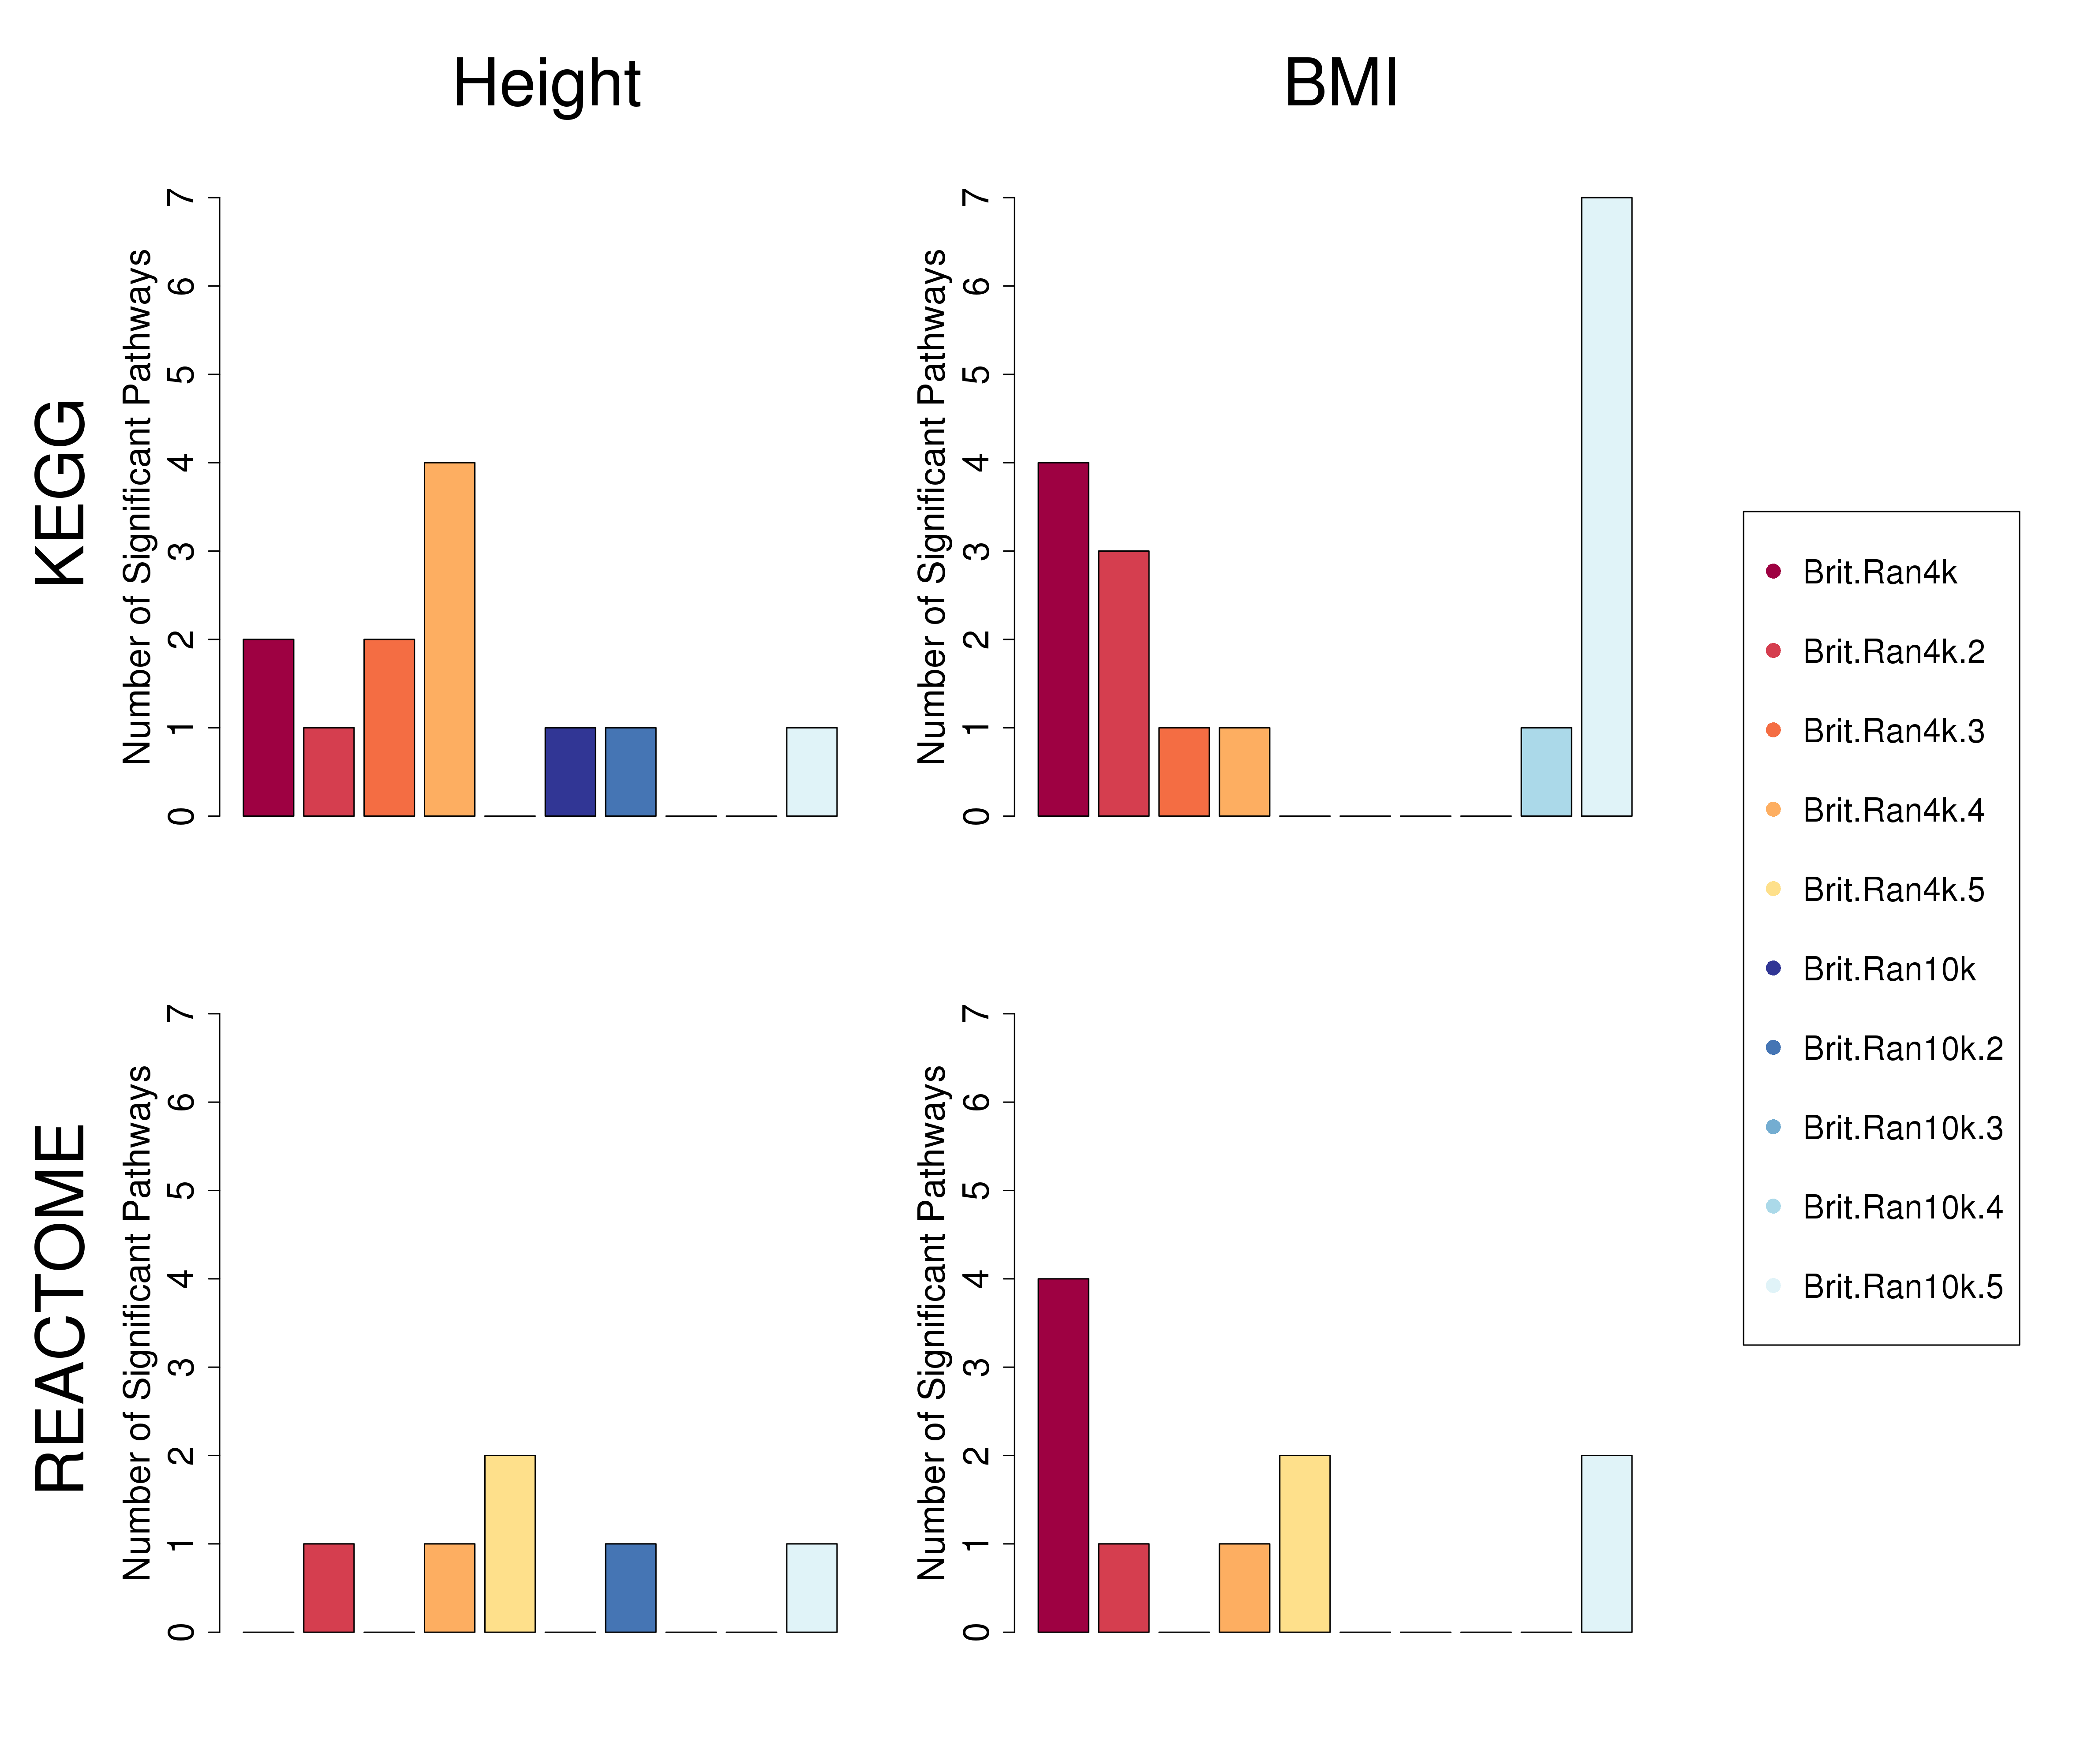
\includegraphics[scale=.45]{Images/Supp/InterPath_Supp_Figure_BritReps_Barplot_vs3.png}
\caption[TBD]{\textbf{Numbers of pathways that have significant marginal epistasis, per British replicate}. The barplots show the number of genome-wide significant pathways found from running MAPIT-R for both height and BMI in the KEGG and REACTOME databases on each of our British subsample replicate populations. Genome-wide significance was determined by using Bonferroni-corrected $p$-value thresholds based on the number of pathways tested in each phenotype, replicate, and pathway database combination. Most replicate runs did not produce many significant results.}
\label{InterPath-Supp-Figure-BritReps-Barplots}
\end{figure}
\clearpage

\newcounter{CharNumber4}
\setcounter{CharNumber4}{1}
\renewcommand{\thefigure}{\arabic{figure}\alph{CharNumber4}}
\begin{landscape}
\begin{figure}[htbp]
\centering
\includegraphics[scale=.2]{Images/Supp/InterPath_Supp_Figure_BritReps_Heatplots_KEGG_vs3.png}
\caption[TBD]{\textbf{Overlap of genome-wide significant MAPIT-R pathways between British replicates subgroups: KEGG}. The heatplots show the numbers of genome-wide significant MAPIT-R pathways that overlap between each British replicate subgroup for height and BMI in the KEGG database. The diagonal shows the total number of genome-wide significant pathways per population subgroup. We do not observe many genome-wide significant pathways or pathways that overlap between replicate subgroups.}
\label{InterPath-Supp-Figure-BritReps-Heatplots-AllPaths-KEGG}
\end{figure}
\clearpage
\addtocounter{figure}{-1}
\addtocounter{CharNumber4}{1}
\end{landscape}

\begin{landscape}
\begin{figure}[htbp]
\centering
\includegraphics[scale=.2]{Images/Supp/InterPath_Supp_Figure_BritReps_Heatplots_REACTOME_vs3.png}
\caption[TBD]{\textbf{Overlap of genome-wide significant MAPIT-R pathways between British replicates subgroups: REACTOME}. The heatplots show the numbers of genome-wide significant MAPIT-R pathways that overlap between each British replicate subgroup for height and BMI in the REACTOME database. The diagonal shows the total number of genome-wide significant pathways per population subgroup. We do not observe many genome-wide significant pathways or pathways that overlap between replicate subgroups.}
\label{InterPath-Supp-Figure-BritReps-Heatplots-AllPaths-REACTOME}
\end{figure}
\clearpage
\end{landscape}
\renewcommand{\thefigure}{\arabic{figure}}

\begin{figure}[htbp]
\centering
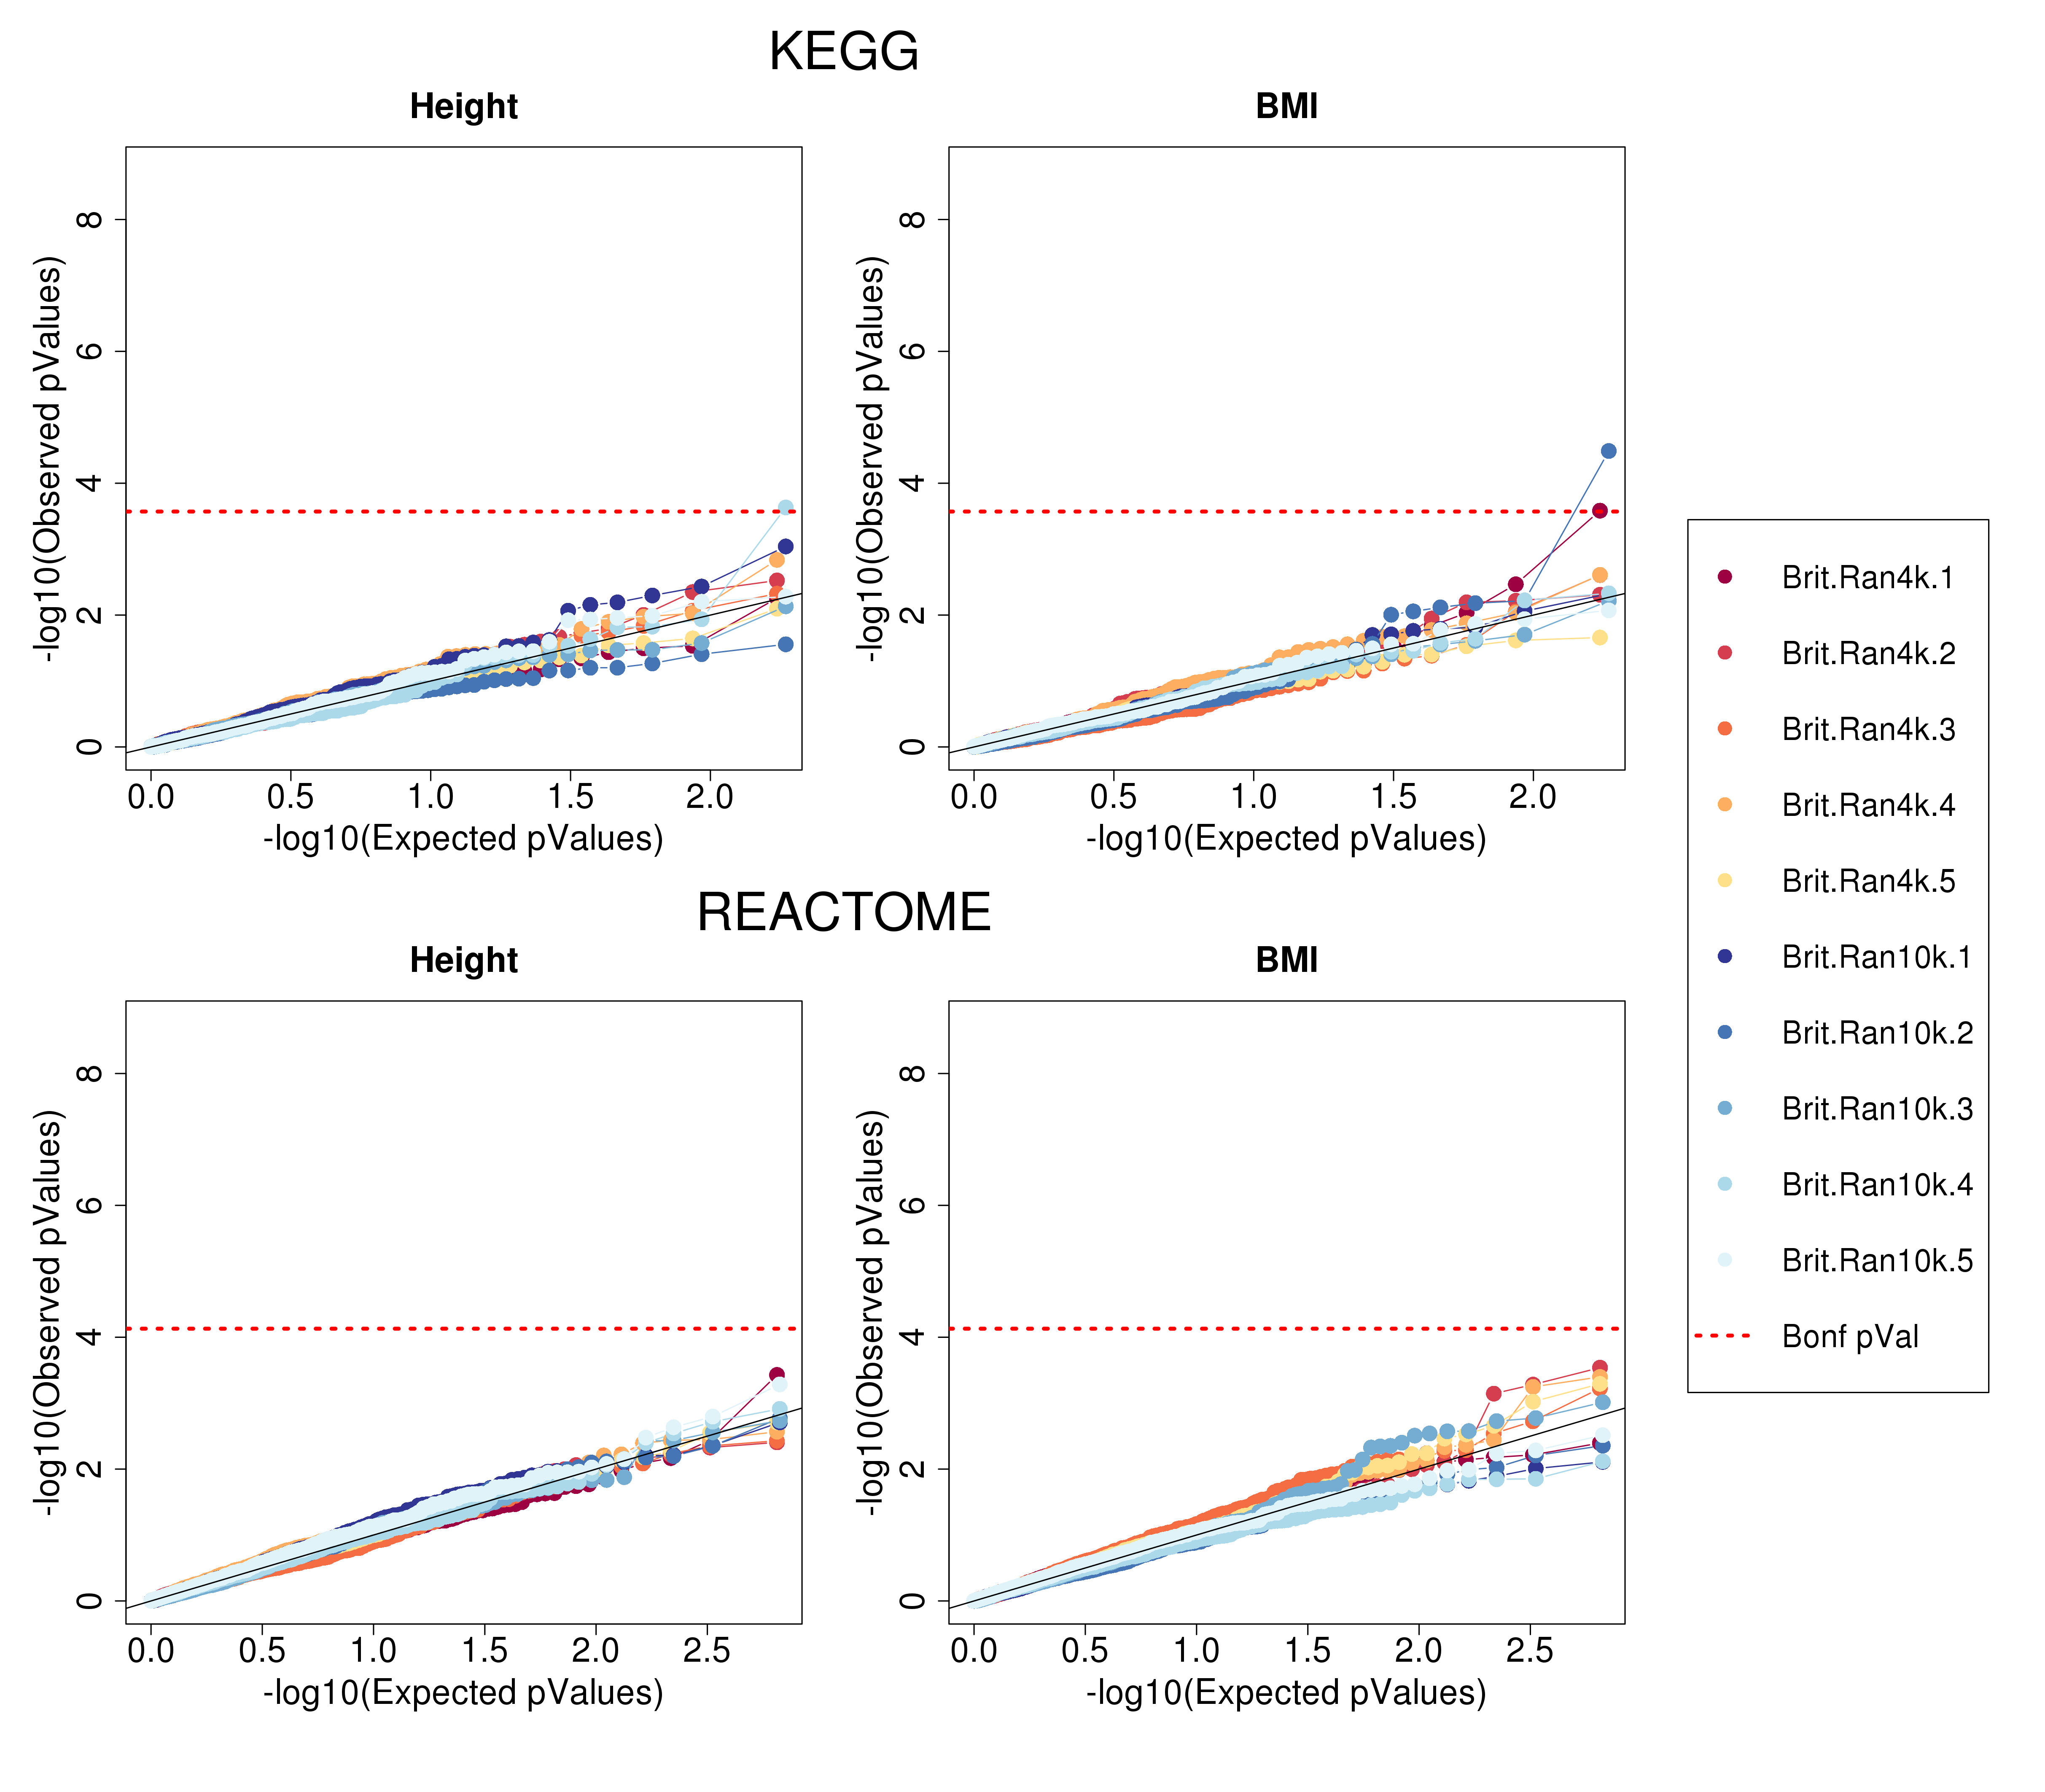
\includegraphics[scale=.35]{Images/Supp/InterPath_Supp_Figure_BritReps_perm1_QQPlots_AllPaths_vs1.png}
\caption[TBD]{\textbf{QQ-Plots of MAPIT-R results using permuted phenotypes, per British replicate}. The figure shows QQ-plots for running MAPIT-R using single, permuted versions of both height and BMI with the KEGG \& REACTOME databases. Phenotypes were permuted within each British replicate subgroup. Shown on the $x$-axis are the -$\log_{10}$ of the expected $p$-values and the on the $y$-axis are on the -$\log_{10}$ of the observed $p$-values. The dotted red line is our Bonferroni-corrected $p$-value threshold based on the number of pathways tested per phenotype and pathway database combination. We find across all replicate, phenotype, and pathway database combinations that MAPIT-R continues to show proper null behavior within the range expected when using permuted phenotypes.}
\label{InterPath-Supp-Figure-BritReps-perm1-QQPlots-AllPaths}
\end{figure}
\clearpage

\newcounter{CharNumber3}
\setcounter{CharNumber3}{1}
%\renewcommand{\thefigure}{\arabic{figure}\alph{CharNumber3}}
\setlength{\footskip}{1cm}
\begin{figure}[htbp]
\centering
\vspace*{-1cm}
\includegraphics[scale=.2]{Images/Supp/InterPath_Supp_Figure_BritReps_pValHists_AllPaths_vs1_pt1.png}
\caption[TBD]{\textbf{$p$-Value histograms of MAPIT-R results using permuted phenotypes, per British replicate}. The figure shows histograms of MAPIT-R $p$-values collected across ten independent phenotype permutation runs for each British Ran4000 and Ran10000 subsample replicate. The same phenotype permutation for a given replicate was used across both pathway databases (i.e. 10 permutations were done for height and 10 done for BMI for each subgroup). Covariates used from the original MAPIT-R analysis were kept the same.}
\label{InterPath-Supp-Figure-BritReps-10perms-pValHists-pt1}
\end{figure}
\clearpage
\setlength{\footskip}{1cm}
\addtocounter{figure}{-1}
\addtocounter{CharNumber3}{1}

\setlength{\footskip}{2cm}
\begin{figure}[htbp]
\centering
\vspace*{-1cm}
\includegraphics[scale=.2]{Images/Supp/InterPath_Supp_Figure_BritReps_pValHists_AllPaths_vs1_pt2.png}
\caption[TBD]{\textbf{$p$-Value histograms of MAPIT-R results using permuted phenotypes, per British replicate}. The figure shows histograms of MAPIT-R $p$-values collected across ten independent phenotype permutation runs for each British Ran4000 and Ran10000 subsample replicate. The same phenotype permutation for a given replicate was used across both pathway databases (i.e. 10 permutations were done for height and 10 done for BMI for each subgroup). Covariates used from the original MAPIT-R analysis were kept the same.}
\label{InterPath-Supp-Figure-BritReps-10perms-pValHists-pt2}
\end{figure}
\clearpage
\setlength{\footskip}{1cm}
%\renewcommand{\thefigure}{\arabic{figure}}

\begin{figure}[htbp]
\centering
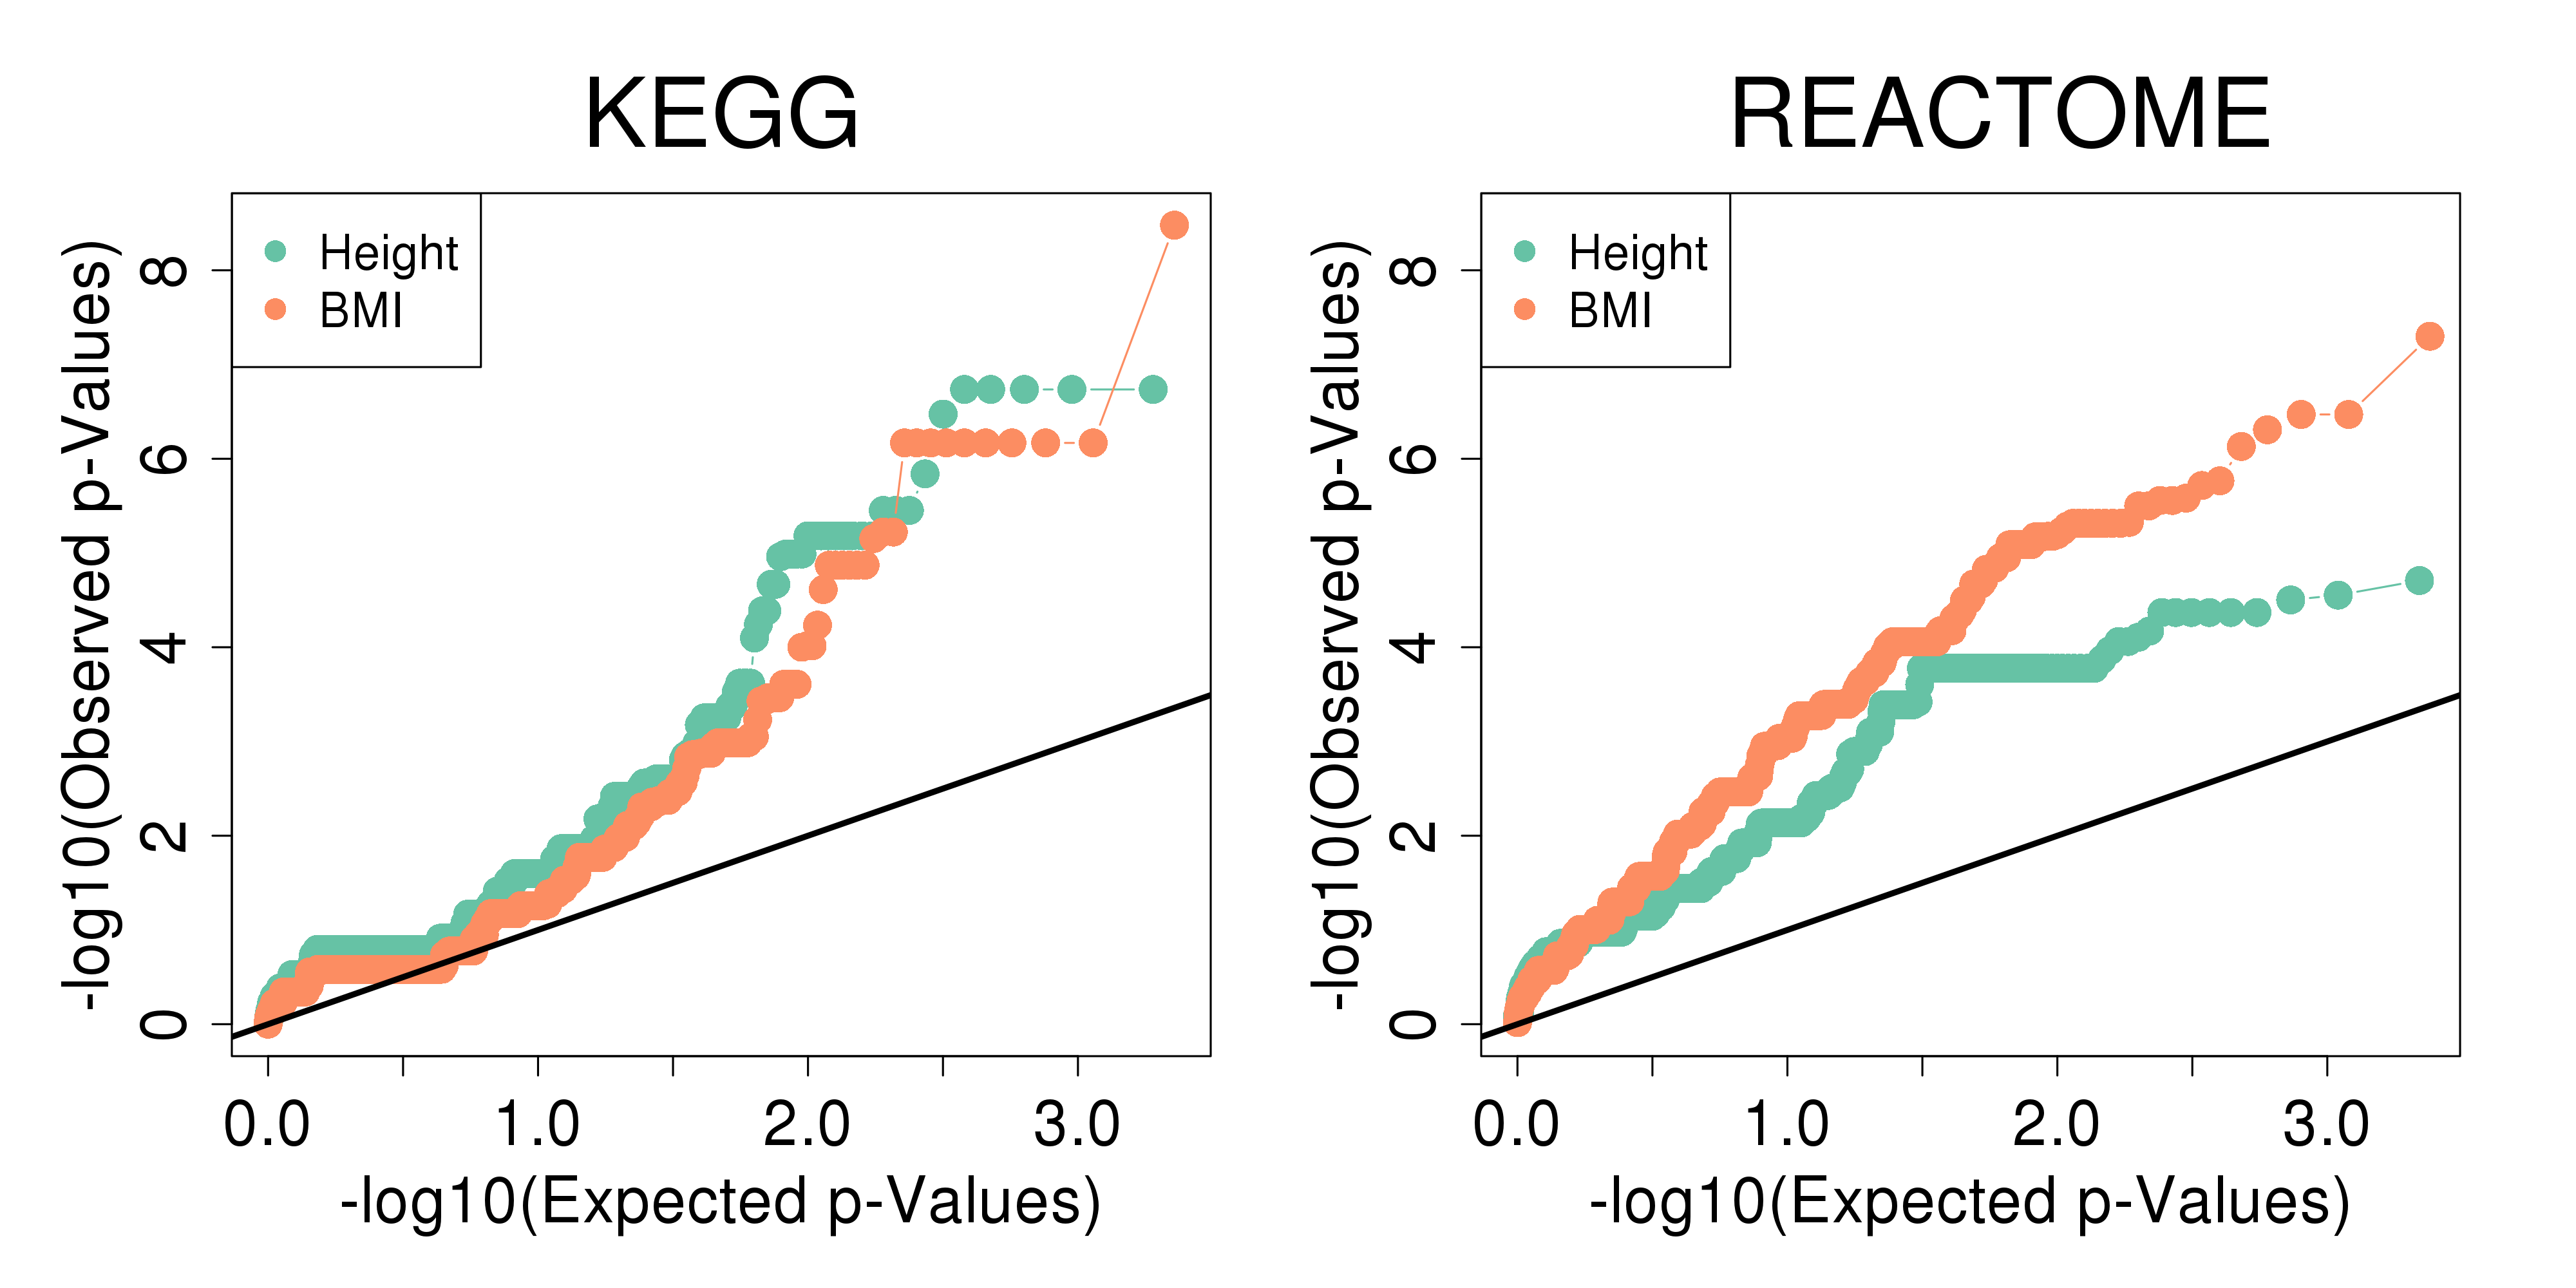
\includegraphics[scale=.45]{Images/Supp/InterPath_Supp_Figure_Hypergeometric_QQPlots_African_vs2.png}
\caption[TBD]{\textbf{QQ-Plots of gene count hypergeometric enrichment test $p$-values in the African subgroup}. The figure shows QQ-plots of the gene count hypergeometric enrichment results for the African subgroup in both height and BMI and across both the KEGG and REACTOME databases. Every gene that was present among the set of MAPIT-R genome-wide significant pathways for that phenotype and pathway database combination was tested, including genes that were only present once. The $x$-axis is the expected -$\log_{10}$ $p$-values and the $y$-axis is the observed -$\log_{10}$ $p$-values. Brown dots are results from the height analysis and purple dots are results from the BMI analysis.}
\label{InterPath-Supp-Figure-Hypergeometric-QQPlots-African}
\end{figure}
\clearpage

%\begin{figure}[htbp]
%\centering
%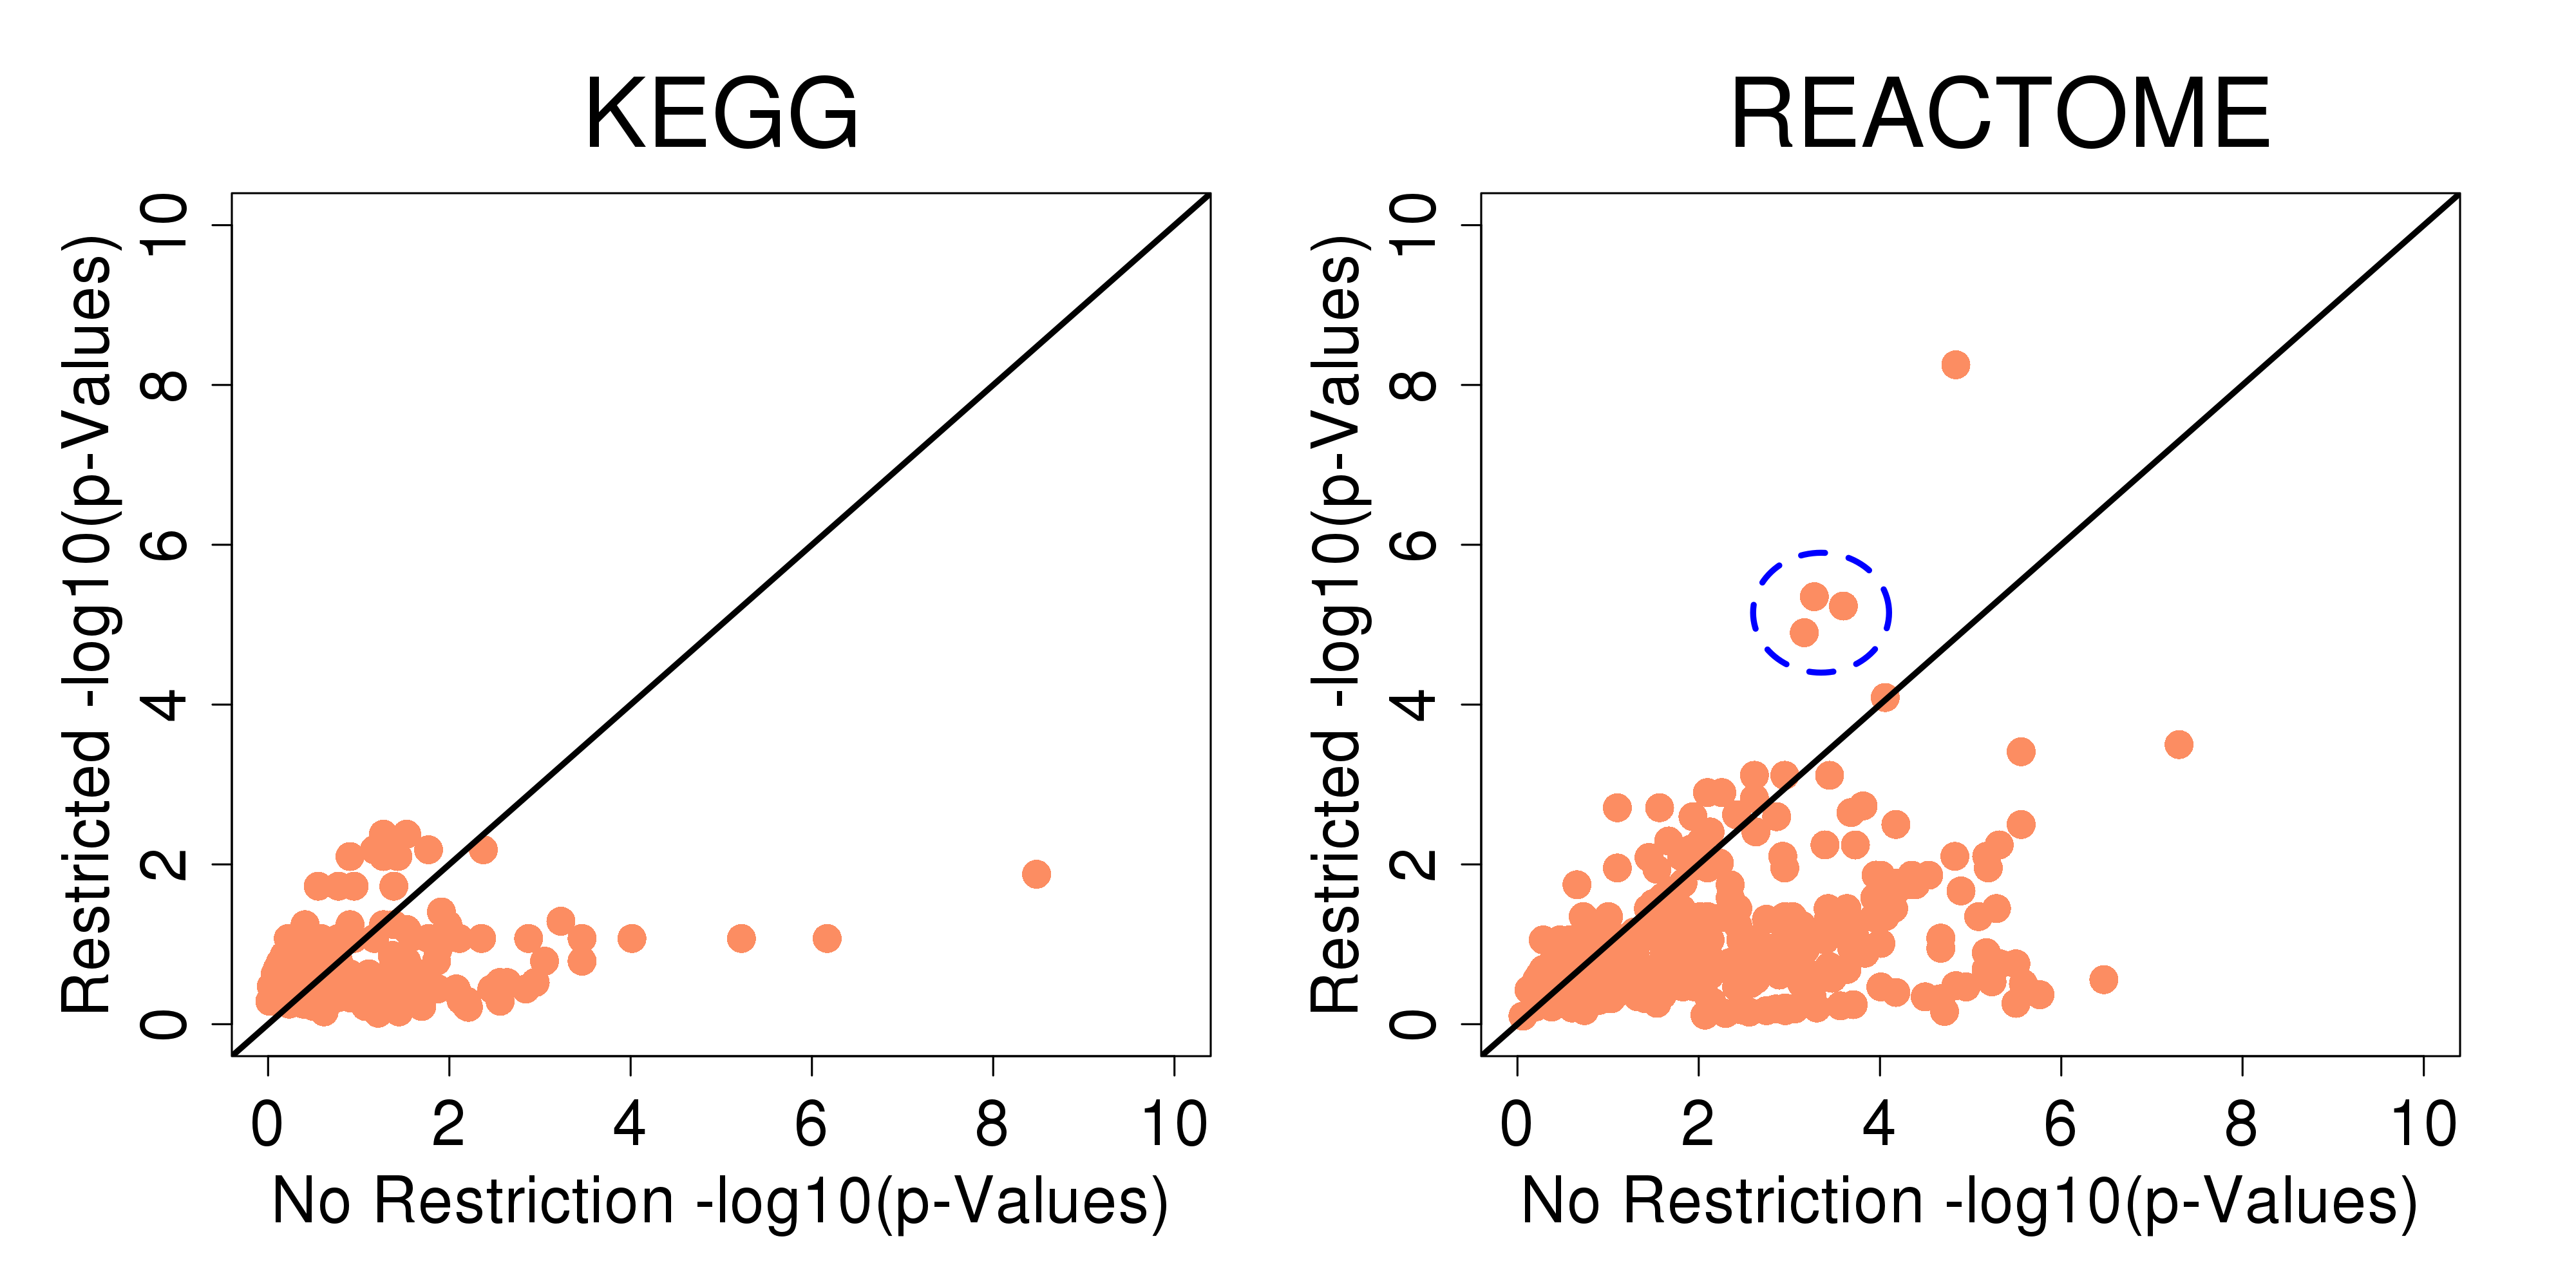
\includegraphics[scale=.45]{Images/Supp/InterPath_Supp_Figure_Hypergeometric_RestrictedComps_African_BMI_vs2.png}
%\caption[TBD]{\textbf{Comparison of gene count hypergeometric enrichment $p$-values in BMI using pathway size restrictions versus no size restrictions in the African subgroup}. The figure shows comparisons of the gene count hypergeometric enrichment $p$-values between the size restricted version of the analysis and the original unrestricted version of the analysis. The size restricted version of the analysis is redoing the hypergeometric enrichment tests but only using pathways that contained $<$ 1,000 SNPs. Only results for BMI are shown here since almost all Bonferroni significant pathways were lost in the height results due to this size restriction step. The $x$-axis shows the original, unrestricted hypergeometric -$\log_{10}$ $p$-values, and the $y$-axis shows the new, size restricted hypergeoemtric -$\log_{10}$ $p$-values. The PSM* gene cluster is highlighted in the REACTOME plot. For lists of the top genes that became more significant due to the size restriction step, see Supplementary Table \ref{InterPath-Supp-Table-Hypergeometric-RestrictedComps-African-BMI-TopExamples}.}
%\label{InterPath-Supp-Figure-Hypergeometric-RestrictedComps-African-BMI}
%\end{figure}
%\clearpage

\setlength{\footskip}{3cm}
\begin{figure}[htbp]
\centering
\vspace*{-2cm}
\includegraphics[scale=.2]{Images/Supp/InterPath_Supp_Figure_IBS_AllPops_vs3.png}
\caption[TBD]{\textbf{Pathway-level genetic diversity versus MAPIT-R results for all phenotype, database, and subgroup combinations}. Caption continued on next page.}
\label{InterPath-Supp-Figure-IBS-AllPops}
\end{figure}
\clearpage
\setlength{\footskip}{1cm}
\addtocounter{figure}{-1}

\begin{figure} [t!]
\caption[TBD]{\textbf{Pathway-level genetic diversity versus MAPIT-R results for all phenotype, database, and subgroup combinations}. The figure shows the mean pairwise IBS proportions per pathway plotted against each pathway's MAPIT-R $p$-value for every UKB subgroup, phenotype, and pathway database combination. IBS proportions were calculated per pathway by using that pathway's set of SNPs, were calculated pairwise between every set of individuals in the subgroup, and then averaged across each of these pairs for a final, single summary metric. We observe across almost every combination no significant relationship between mean pairwise IBS proportion and MAPIT-R $p$-value.}
\label{InterPath-Supp-Figure-IBS-AllPops-Caption}
\end{figure}
\clearpage

\begin{figure}[htbp]
\centering
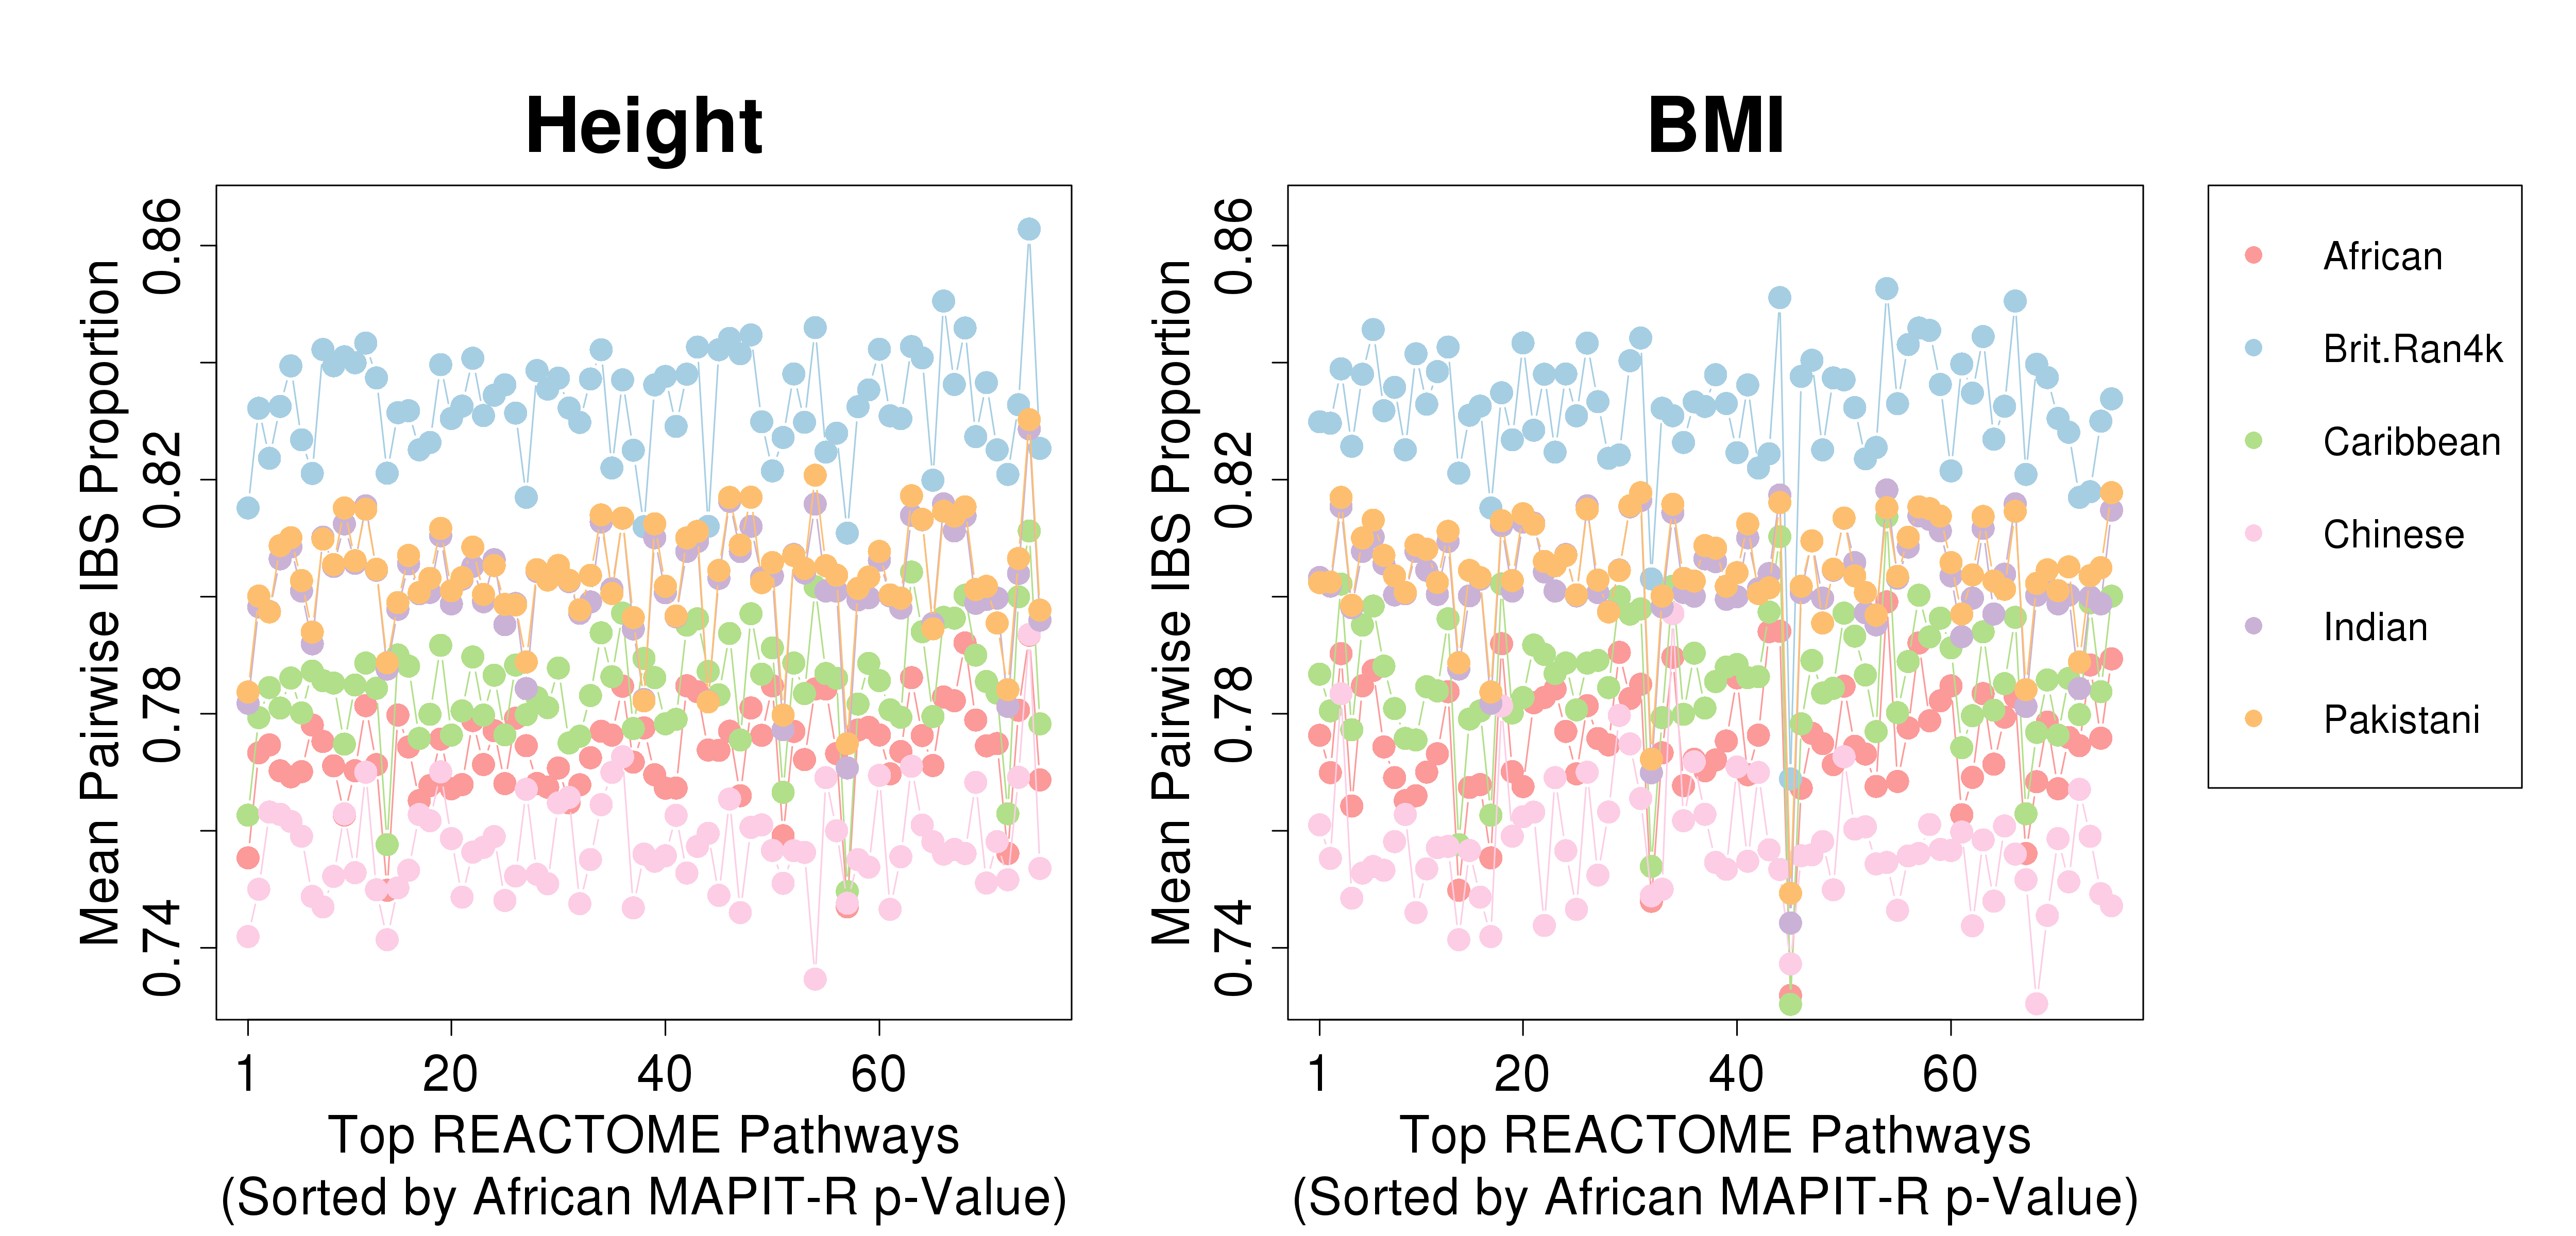
\includegraphics[scale=.35]{Images/Supp/InterPath_Supp_Figure_IBS_AllPopComps_vs3_REACTOME.png}
\caption[TBD]{\textbf{Pathway-level genetic diversity across all UKB subgroups for top African MAPIT-R REACTOME pathways}. The figure plots the mean pairwise IBS proportions of each UKB subgroup for the top 75 REACTOME pathways (sorted by MAPIT-R African subgroup $p$-value) for each phenotype and pathway database combination. Most variation in mean pairwise IBS proportions varies moreso based on the pathways themselves and not on ancestry; subgroups differ between one another mostly at the same levels across each pathway.}
\label{InterPath-Supp-Figure-IBS-AllPopComps-REACTOME}
\end{figure}
\clearpage


\setlength{\footskip}{3cm}
\begin{figure}[htbp]
\centering
\vspace*{-2cm}
\includegraphics[scale=.2]{Images/Supp/InterPath_Supp_Figure_PC1Loading_AllPaths_vs1.png}
\caption[TBD]{\textbf{Relationship between MAPIT-R $p$-values and proportions of pathway SNPs loaded on PC1, all pathways}. Caption continued on next page.}
\label{InterPath-Supp-Figure-PC1Loading-AllPaths}
\end{figure}
\clearpage
\setlength{\footskip}{1cm}

\addtocounter{figure}{-1}
\begin{figure} [t!]
  \caption{\textbf{Relationship between MAPIT-R $p$-values and proportions of pathway SNPs loaded on PC1, all subgroups}. }
\label{InterPath-Supp-Figure-PC1Loading-AllPaths-Caption}
\end{figure}
\clearpage

\section{Supplementary Tables}\label{Supplementary-Tables}

\begin{table}[ht]
\centering
\begin{tabular}{ccccc}
  \hline
\textbf{UK BioBank} & \textbf{Individuals} & \textbf{SNPs} & \textbf{KEGG} & \textbf{REACTOME} \\
\textbf{subgroup} & & & \textbf{Pathways} & \textbf{Pathways}  \\
  \hline
\textbf{Original subgroups:} & & & & \\
African & 3111 & 374466 & 180 & 658 \\ 
British.Ran4000 & 3848 & 600006 & 173 & 650 \\ 
Caribbean & 3833 & 410017 & 181 & 661 \\ 
Chinese & 1448 & 345221 & 153 & 626 \\ 
Indian & 5077 & 505854 & 181 & 662 \\ 
Pakistani & 1581 & 516806 & 141 & 596 \\ 
\\
\textbf{British Replicates:} & & & & \\
British.Ran4000.2 & 3869 & 599381 & 173 & 650 \\ 
British.Ran4000.3 & 3836 & 600654 & 173 & 649 \\ 
British.Ran4000.4 & 3838 & 599829 & 173 & 650 \\ 
British.Ran4000.5 & 3853 & 599442 & 173 & 650 \\ 
British.Ran10000 & 9603 & 597298 & 186 & 669 \\ 
British.Ran10000.2 & 9628 & 597577 & 186 & 669 \\ 
British.Ran10000.3 & 9636 & 597486 & 186 & 669 \\ 
British.Ran10000.4 & 9593 & 597369 & 186 & 669 \\ 
British.Ran10000.5 & 9596 & 597507 & 186 & 669 \\ 
  \hline
\end{tabular}
\caption[TBD]{\textbf{UK BioBank subgroup and British replicate statistics}. The table shows various statistics for each group of UKB subgroups that were analyzed in this study. `Original subgroups' refers to the multiple global human ancestries that were initially analyzed at the beginning of this study, and `British Replicates' refers specifically to the subgroups that were created to analyze multiple, independent random subsamples of the UKB British cohort. The number of individuals and SNPs post quality-control used are shown in the second and third columns, and the number of KEGG and REACTOME pathways analyzed in each subgroup are shown in the fourth and fifth columns. Note that for the `British Replicates' subgroups each group began with an independent set of either 4,000 or 10,000 individuals from the original UKB phenotype file.}
\label{InterPath-Supp-Table-UKBPopStats}
\end{table}
\clearpage

%Irish & 11575 & 588324 & 186 & 671 \\ 

\begin{landscape}
\setlength{\footskip}{2cm}
\begin{table}[ht]
\centering
\begin{tabular}{ccccccc}
  \hline
  \textbf{Trait} & \textbf{African} & & \textbf{British.Ran4k} & & \textbf{Caribbean} & \\ 
& \textbf{Chr:BP} & \textbf{Proportion} & \textbf{Chr:BP} & \textbf{Proportion} & \textbf{Chr:BP} & \textbf{Proportion} \\ 
  \hline
\textbf{Height:} & & & & & & \\
& 9:8851248 & 0.402 & 2:68593134 & 0.434 & 3:115845348 & 0.352 \\
  & 2:192167280 & 0.301 & 11:33992648 & 0.350 & 4:142116338 & 0.329 \\ 
  & 20:11424166 & 0.291 & 1:19440383 & 0.270 & 16:11185464 & 0.246 \\ 
  & 15:25999954 & 0.271 & 11:12738444 & 0.258 & 7:38160558 & 0.240 \\ 
  & 8:4275585 & 0.256 & 12:129932700 & 0.212 & 4:84952912 & 0.237 \\ 
  & 7:111551740 & 0.247 & 10:129548670 & 0.209 & 20:42387041 & 0.213 \\ 
  & 7:5894502 & 0.245 & 7:126672487 & 0.193 & 5:138942117 & 0.208 \\ 
  & 20:42387041 & 0.221 & 11:12674963 & 0.187 & 8:27895386 & 0.205 \\ 
  & 11:56631974 & 0.213 & 9:23129565 & 0.176 & 19:43701423 & 0.198 \\ 
  & 8:116901222 & 0.213 & 20:55953947 & 0.170 & 6:834751 & 0.196 \\ 
  \\
\textbf{BMI:} & & & & & & \\
& 16:26051170 & 0.230 & 2:27075505 & 0.293 & 12:99313419 & 0.319 \\ 
  & 5:172707503 & 0.228 & 1:107460560 & 0.267 & 5:70798541 & 0.284 \\ 
  & 11:2699051 & 0.208 & 21:16339852 & 0.212 & 2:34625180 & 0.273 \\ 
  & 5:16862840 & 0.207 & 2:223779979 & 0.189 & 1:221101692 & 0.266 \\ 
  & 8:48411885 & 0.202 & 2:162386309 & 0.189 & 14:51994228 & 0.235 \\ 
  & 10:133143956 & 0.198 & 2:138690969 & 0.189 & 10:131663327 & 0.234 \\ 
  & 15:93657838 & 0.192 & 16:83246883 & 0.177 & 1:56414458 & 0.225 \\ 
  & 16:55172951 & 0.191 & 13:90223042 & 0.174 & 5:93403619 & 0.220 \\ 
  & 17:32754797 & 0.184 & 13:92829268 & 0.163 & 2:177527111 & 0.219 \\ 
  & 6:1011570 & 0.168 & 6:100900508 & 0.157 & 1:85416840 & 0.218 \\
   \hline
\end{tabular}
\caption[TBD]{\textbf{Lists of SNPs with the largest proportions of marginally significant PLINK pairwise epistasis tests, per subgroup}. Caption continued at the end of the table.}
\label{InterPath-Supp-Table-PLINK-Proportions-TopSNPs-a}
\end{table}
\end{landscape}
\clearpage
\setlength{\footskip}{1cm}
\addtocounter{table}{-1}

\begin{landscape}
\setlength{\footskip}{2cm}
\begin{table}[ht]
\centering
\begin{tabular}{ccccccc}
  \hline
  \textbf{Trait} & \textbf{Chinese} & & \textbf{Indian} & & \textbf{Pakistani} & \\ 
& \textbf{Chr:BP} & \textbf{Proportion} & \textbf{Chr:BP} & \textbf{Proportion} & \textbf{Chr:BP} & \textbf{Proportion} \\ 
  \hline
\textbf{Height:} & & & & & & \\
& 6:74098688 & 1.025 & 8:22014852 & 0.203 & 3:25962790 & 1.015 \\
  & 7:19736280 & 0.503 & 2:135138136 & 0.190 & 11:33951568 & 0.953 \\ 
  & 17:74993606 & 0.493 & 11:55110903 & 0.190 & 1:61014885 & 0.616 \\ 
  & 7:150512307 & 0.491 & 2:181346849 & 0.180 & 18:18905020 & 0.580 \\ 
  & 7:95703904 & 0.461 & 2:181318303 & 0.167 & 12:119540062 & 0.573 \\ 
  & 17:8135061 & 0.416 & 1:159947480 & 0.159 & 8:145948440 & 0.558 \\ 
  & 19:2500027 & 0.413 & 1:18062545 & 0.157 & 22:44643912 & 0.539 \\ 
  & 7:95696930 & 0.408 & 8:86425809 & 0.153 & 5:175433876 & 0.491 \\ 
  & 8:89565212 & 0.401 & 5:44725795 & 0.151 & 11:101951678 & 0.488 \\ 
  & 14:86697878 & 0.399 & 5:167366400 & 0.149 & 12:119554751 & 0.486 \\
  \\
\textbf{BMI:} & & & & & & \\
& 3:74946238 & 0.692 & 6:131708393 & 0.169 & 1:24690676 & 0.872 \\ 
  & 17:65485380 & 0.689 & 11:90267176 & 0.166 & 2:30702842 & 0.458 \\ 
  & 3:116001766 & 0.496 & 3:75936499 & 0.165 & 7:29191481 & 0.448 \\ 
  & 3:30814425 & 0.470 & 5:73129149 & 0.162 & 4:167120342 & 0.431 \\ 
  & 5:117528365 & 0.395 & 13:74840677 & 0.153 & 18:45616828 & 0.411 \\ 
  & 3:75050057 & 0.370 & 12:68110089 & 0.150 & 15:90686924 & 0.406 \\ 
  & 20:55362831 & 0.354 & 11:92390082 & 0.146 & 11:131792814 & 0.391 \\ 
  & 22:22359389 & 0.338 & 4:63750280 & 0.142 & 5:83958603 & 0.379 \\ 
  & 10:85864069 & 0.332 & 18:10853771 & 0.141 & 7:152693740 & 0.375 \\ 
  & 3:75064460 & 0.320 & 16:6860576 & 0.140 & 10:110657497 & 0.371 \\ 
   \hline
\end{tabular}
\caption[TBD]{\textbf{Lists of SNPs with the largest proportions of marginally significant PLINK pairwise epistasis tests, per subgroup}. Caption continued at the end of the table.}
\label{InterPath-Supp-Table-PLINK-Proportions-TopSNPs-b}
\end{table}
\end{landscape}
\clearpage
\setlength{\footskip}{1cm}
\addtocounter{table}{-1}

\begin{table} [t!]
  \caption{\textbf{Lists of SNPs with the largest proportions of marginally significant PLINK pairwise epistasis tests, per subgroup}. The table shows the top 10 SNPs in terms of proportion of marginally significant PLINK pairwise epistatic interactions for height and BMI in each of our UKB subgroups. Marginal significance is determined by a PLINK pairwise SNP interaction $p$-value being below $1\times10^{-4}$. For each UKB subgroup the first column lists the chromosome and basepair position for the SNP of interest and the second column lists the PLINK test proportions.}
\label{InterPath-Supp-Table-PLINK-Proportions-TopSNPs-Caption}
\end{table}
\clearpage

\begin{landscape}
\setlength{\footskip}{2cm}
\begin{table}[ht]
\centering
\begin{tabular}{ccccccc}
  \hline
  \textbf{Trait} & \textbf{African} & & \textbf{British.Ran4k} & & \textbf{Caribbean} & \\ 
& \textbf{Chr:BP} & \textbf{-$\log_{10}$($p$)} & \textbf{Chr:BP} & \textbf{-$\log_{10}$($p$)} & \textbf{Chr:BP} & \textbf{-$\log_{10}$($p$)} \\ 
  \hline
\textbf{Height:} & & & & & & \\
& 15:98255395 & 6.064 & 15:40308859 & 5.654 & 10:102705058 & 6.366 \\ 
  & 21:33179371 & 5.947 & 20:18929160 & 5.206 & 10:102754238 & 6.167 \\ 
  & 7:107441154 & 5.633 & 2:68593134 & 5.175 & 11:60876561 & 5.899 \\ 
  & 22:50883961 & 5.292 & 15:40284523 & 4.941 & 10:102738551 & 5.787 \\ 
  & 20:10633313 & 5.234 & 17:34817693 & 4.866 & 2:29225504 & 5.778 \\ 
  & 7:28263825 & 5.221 & 17:34833820 & 4.863 & 10:102746503 & 5.736 \\ 
  & 15:43423327 & 4.928 & 11:33992648 & 4.859 & 4:38155825 & 5.631 \\ 
  & 7:12077909 & 4.794 & 13:37130549 & 4.778 & 12:28230120 & 5.494 \\ 
  & 6:75947027 & 4.764 & 13:23471815 & 4.750 & 8:32275265 & 5.380 \\ 
  & 1:49180331 & 4.763 & 4:46199808 & 4.641 & 16:78704199 & 5.296 \\ 
   \\
\textbf{BMI:} & & & & & & \\
& 16:54243548 & 6.119 & 4:153811650 & 5.119 & 1:177923440 & 6.536 \\ 
  & 18:24501383 & 5.818 & 18:20190795 & 5.068 & 16:21710678 & 5.922 \\ 
  & 2:233554499 & 5.402 & 1:104061746 & 5.063 & 9:130479233 & 5.843 \\ 
  & 3:10899881 & 5.345 & 4:153690842 & 4.901 & 4:8332861 & 5.702 \\ 
  & 18:68624629 & 5.330 & 8:107630040 & 4.877 & 22:39830123 & 5.652 \\ 
  & 2:5257185 & 5.048 & 21:21535472 & 4.866 & 5:123252456 & 5.564 \\ 
  & 10:48485976 & 4.868 & 11:127409790 & 4.780 & 6:35705892 & 5.445 \\ 
  & 11:19838292 & 4.850 & 1:183277665 & 4.779 & 1:234364335 & 5.419 \\ 
  & 5:172707503 & 4.715 & 2:122598583 & 4.779 & 2:66821247 & 5.396 \\ 
  & 4:38789675 & 4.713 & 20:5478313 & 4.773 & 1:221101692 & 5.379 \\ 
   \hline
\end{tabular}
\caption[TBD]{\textbf{Lists of SNPs with the most significant MAPIT $p$-values, per subgroup}. Caption continued at the end of the table.}
\label{InterPath-Supp-Table-MAPIT-TopSNPs-a}
\end{table}
\end{landscape}
\clearpage
\setlength{\footskip}{1cm}
\addtocounter{table}{-1}

\begin{landscape}
\setlength{\footskip}{2cm}
\begin{table}[ht]
\centering
\begin{tabular}{ccccccc}
  \hline
  \textbf{Trait} & \textbf{Chinese} & & \textbf{Indian} & & \textbf{Pakistani} & \\ 
& \textbf{Chr:BP} & \textbf{-$\log_{10}$($p$)} & \textbf{Chr:BP} & \textbf{-$\log_{10}$($p$)} & \textbf{Chr:BP} & \textbf{-$\log_{10}$($p$)} \\ 
  \hline
\textbf{Height:} & & & & & & \\
& 4:101070872 & 5.673 & 11:30478524 & 5.869 & 14:84654448 & 5.562 \\ 
  & 9:84390158 & 5.453 & 11:30452281 & 5.546 & 2:177358580 & 4.986 \\ 
  & 19:2500027 & 5.329 & 11:30564908 & 5.443 & 2:64556555 & 4.814 \\ 
  & 13:20836940 & 5.224 & 10:121732871 & 5.399 & 6:52476643 & 4.774 \\ 
  & 4:159328540 & 5.073 & 5:151876334 & 5.351 & 3:9071220 & 4.767 \\ 
  & 10:45368032 & 4.979 & 19:53154530 & 5.304 & 6:14814367 & 4.740 \\ 
  & 6:113595727 & 4.927 & 13:19745579 & 5.223 & 1:168609132 & 4.631 \\ 
  & 4:101059291 & 4.773 & 5:158867212 & 5.198 & 16:61560661 & 4.626 \\ 
  & 10:72763749 & 4.682 & 12:32084875 & 5.138 & 7:80071426 & 4.625 \\ 
  & 3:187622081 & 4.619 & 6:46375132 & 5.120 & 8:60021908 & 4.586 \\ 
   \\
\textbf{BMI:} & & & & & & \\
& 11:97016249 & 5.184 & 2:2116870 & 6.096 & 22:25096704 & 5.147 \\ 
  & 10:12681042 & 4.961 & 8:65989176 & 6.025 & 17:12707766 & 4.907 \\ 
  & 21:34354062 & 4.809 & 6:29702709 & 5.920 & 7:10580190 & 4.778 \\ 
  & 4:14390603 & 4.736 & 6:29700079 & 5.729 & 10:73300992 & 4.744 \\ 
  & 4:14386866 & 4.643 & 6:29700615 & 5.729 & 13:42116031 & 4.652 \\ 
  & 7:73145015 & 4.642 & 4:102205385 & 5.634 & 19:13980805 & 4.402 \\ 
  & 4:14390228 & 4.618 & 7:29413388 & 5.440 & 15:25980875 & 4.350 \\ 
  & 4:14385522 & 4.587 & 3:54409526 & 5.431 & 3:32802690 & 4.328 \\ 
  & 10:122226568 & 4.586 & 8:130332722 & 5.341 & 5:133848660 & 4.304 \\ 
  & 1:33714603 & 4.576 & 8:4656695 & 5.210 & 6:40366427 & 4.296 \\ 
   \hline
\end{tabular}
\caption[TBD]{\textbf{Lists of SNPs with the most significant MAPIT $p$-values, per subgroup}. Caption continued at the end of the table.}
\label{InterPath-Supp-Table-MAPIT-TopSNPs-b}
\end{table}
\end{landscape}
\clearpage
\setlength{\footskip}{1cm}
\addtocounter{table}{-1}

\begin{table} [t!]
  \caption{\textbf{Lists of SNPs with the most significant MAPIT $p$-values, per subgroup}. The table shows the top 10 SNPs for each of our MAPIT analyses on height and BMI in our UKB subgroups. For each UKB subgroup the first column lists the chromosome and basepair position for the SNP of interest and the second column lists the MAPIT -$\log_{10}$ $p$-value for that SNP. No single SNP reaches genome-wide significance ($p$-value $< 5\times10^{-8}$).}
\label{InterPath-Supp-Table-MAPIT-TopSNPs-Caption}
\end{table}
\clearpage

%From: https://tex.stackexchange.com/questions/118606/numbering-tables-a1-a2-etc-in-latex & https://tex.stackexchange.com/questions/83689/next-subsequent-letter-in-the-alphabet
\newcounter{CharNumber1}
\setcounter{CharNumber1}{1}
\renewcommand{\thetable}{\arabic{table}\alph{CharNumber1}}
\setlength{\footskip}{2cm}
\begin{landscape}
\begin{table}[ht]
\centering
\vspace*{-.75cm}
\begin{tabular}{lccc}
  \hline
\textbf{Population \& Pathway} & \textbf{Genes} & \textbf{SNPs} & \textbf{$p$-Value} \\ 
  \hline
  \textbf{African:} & & & \\
 KEGG\_CHEMOKINE\_SIGNALING\_PATHWAY & 170 & 2448 & 5.136E-10 \\
 KEGG\_AXON\_GUIDANCE & 120 & 3045 & 1.511E-08 \\ 
  KEGG\_HYPERTROPHIC\_CARDIOMYOPATHY\_HCM & 77 & 2132 & 1.542E-08 \\ 
  KEGG\_CYTOKINE\_CYTOKINE\_RECEPTOR\_INTERACTION & 234 & 2279 & 2.837E-08 \\ 
  KEGG\_PURINE\_METABOLISM & 135 & 2411 & 1.186E-07 \\ 
  KEGG\_DILATED\_CARDIOMYOPATHY & 83 & 2234 & 1.242E-07 \\ 
  KEGG\_TYPE\_I\_DIABETES\_MELLITUS & 38 & 1659 & 1.330E-07 \\ 
  KEGG\_ENDOCYTOSIS & 169 & 2981 & 1.523E-07 \\ 
  KEGG\_OLFACTORY\_TRANSDUCTION & 365 & 3110 & 1.194E-06 \\ 
  KEGG\_AUTOIMMUNE\_THYROID\_DISEASE & 48 & 1504 & 1.492E-06 \\ 
  KEGG\_NATURAL\_KILLER\_CELL\_MEDIATED\_CYTOTOXICITY & 127 & 2216 & 5.160E-06 \\ 
  KEGG\_ALZHEIMERS\_DISEASE & 136 & 1846 & 5.188E-06 \\ 
  KEGG\_WNT\_SIGNALING\_PATHWAY & 141 & 2050 & 6.536E-06 \\ 
  KEGG\_ALLOGRAFT\_REJECTION & 32 & 1329 & 8.152E-06 \\ 
  KEGG\_HUNTINGTONS\_DISEASE & 148 & 1660 & 8.639E-06 \\ 
  KEGG\_GRAFT\_VERSUS\_HOST\_DISEASE & 35 & 1348 & 8.933E-06 \\ 
  KEGG\_GAP\_JUNCTION & 85 & 1851 & 9.300E-06 \\ 
  KEGG\_SYSTEMIC\_LUPUS\_ERYTHEMATOSUS & 111 & 1525 & 1.499E-05 \\ 
  KEGG\_VIRAL\_MYOCARDITIS & 64 & 1972 & 1.889E-05 \\ 
  KEGG\_ANTIGEN\_PROCESSING\_AND\_PRESENTATION & 74 & 1598 & 2.890E-05 \\ 
  KEGG\_LONG\_TERM\_POTENTIATION & 63 & 1585 & 3.317E-05 \\ 
  KEGG\_INTESTINAL\_IMMUNE\_NETWORK\_FOR\_IGA\_PRODUCTION & 43 & 1072 & 3.838E-05 \\ 
  KEGG\_PHOSPHATIDYLINOSITOL\_SIGNALING\_SYSTEM & 75 & 1681 & 4.497E-05 \\ 
  KEGG\_ARRHYTHMOGENIC\_RIGHT\_VENTRICULAR\_CARDIOMYOPATHY\_ARVC & 70 & 2373 & 5.289E-05 \\ 
  KEGG\_LONG\_TERM\_DEPRESSION & 66 & 1741 & 5.553E-05 \\ 
  KEGG\_GLIOMA & 64 & 974 & 5.649E-05 \\ 
  KEGG\_VASCULAR\_SMOOTH\_MUSCLE\_CONTRACTION & 106 & 2465 & 1.881E-04 \\ 
  KEGG\_REGULATION\_OF\_ACTIN\_CYTOSKELETON & 194 & 3047 & 1.951E-04 \\ 
  KEGG\_TYPE\_II\_DIABETES\_MELLITUS & 45 & 979 & 2.687E-04 \\ 
   \hline
\end{tabular}
\caption[TBD]{\textbf{Lists of genome-wide significant MAPIT-R KEGG pathways in height, per subgroup}. Caption continued at end of tables.}
\label{InterPath-Supp-Table-TopPathways-KEGG-Height-a}
\end{table}
\addtocounter{table}{-1}
%\addtocounter{CharNumber1}{1}
\clearpage

\begin{table}[ht]
\centering
\vspace*{-.75cm}
\begin{tabular}{lccc}
  \hline
  \textbf{British.Ran4000:} & & & \\
  KEGG\_ERBB\_SIGNALING\_PATHWAY & 83 & 2674 & 1.003E-05 \\
KEGG\_TYPE\_I\_DIABETES\_MELLITUS &  39 & 1924 & 1.693E-05 \\ 
 \textcolor{white}{KEGG\_ARRHYTHMOGENIC\_RIGHT\_VENTRICULAR\_CARDIOMYOPATHY\_ARVC } & & & \\
 \textbf{Caribbean:} & & & \\
 KEGG\_CHEMOKINE\_SIGNALING\_PATHWAY & 171 & 2688 & 2.733E-06 \\
 KEGG\_NATURAL\_KILLER\_CELL\_MEDIATED\_CYTOTOXICITY & 128 & 2356 & 1.125E-05 \\
  KEGG\_CELL\_ADHESION\_MOLECULES\_CAMS & 120 & 4029 & 1.770E-05 \\
  KEGG\_LEUKOCYTE\_TRANSENDOTHELIAL\_MIGRATION & 105 & 1941 & 2.169E-05 \\
  KEGG\_VASCULAR\_SMOOTH\_MUSCLE\_CONTRACTION & 106 & 2708 & 3.675E-05 \\
  KEGG\_AXON\_GUIDANCE & 120 & 3365 & 1.088E-04 \\
  KEGG\_SMALL\_CELL\_LUNG\_CANCER & 78 & 1931 & 1.369E-04 \\
  KEGG\_ARRHYTHMOGENIC\_RIGHT\_VENTRICULAR\_CARDIOMYOPATHY\_ARVC & 70 & 2581 & 1.376E-04 \\
  KEGG\_HYPERTROPHIC\_CARDIOMYOPATHY\_HCM & 77 & 2298 & 1.960E-04 \\
 \\
 \textbf{Chinese:} & & & \\
 KEGG\_TYPE\_I\_DIABETES\_MELLITUS & 39 & 1573 & 1.269E-08 \\
 KEGG\_ANTIGEN\_PROCESSING\_AND\_PRESENTATION & 75 & 1505 & 8.287E-08 \\
  KEGG\_MELANOGENESIS & 96 & 1382 & 1.028E-05 \\
  KEGG\_ALLOGRAFT\_REJECTION & 33 & 1250 & 1.183E-05 \\
  KEGG\_GRAFT\_VERSUS\_HOST\_DISEASE & 37 & 1274 & 2.424E-05 \\
  KEGG\_NON\_SMALL\_CELL\_LUNG\_CANCER & 53 & 1081 & 5.337E-05 \\
  KEGG\_SYSTEMIC\_LUPUS\_ERYTHEMATOSUS & 109 & 1399 & 1.252E-04 \\
 \\
 \textbf{Indian:} & & & \\
 KEGG\_NON\_SMALL\_CELL\_LUNG\_CANCER & 53 & 1696 & 4.182E-05 \\
 KEGG\_CYTOKINE\_CYTOKINE\_RECEPTOR\_INTERACTION & 237 & 2995 & 4.965E-05 \\
  KEGG\_REGULATION\_OF\_ACTIN\_CYTOSKELETON & 193 & 4069 & 1.963E-04 \\
  KEGG\_ERBB\_SIGNALING\_PATHWAY & 83 & 2174 & 2.128E-04 \\
   \hline
\end{tabular}
\caption[TBD]{\textbf{Lists of genome-wide significant MAPIT-R KEGG pathways in height, per subgroup}. Continued. \\ }
\label{InterPath-Supp-Table-TopPathways-KEGG-Height-b}
\end{table}
\addtocounter{table}{-1}
%\addtocounter{CharNumber1}{1}

\begin{table}[ht]
\centering
\vspace*{-.75cm}
\begin{tabular}{lccc}
  \hline
 \textbf{Pakistani:} & & & \\
 KEGG\_ANTIGEN\_PROCESSING\_AND\_PRESENTATION & 78 & 1775 & 1.581E-08 \\
 KEGG\_AMINO\_SUGAR\_AND\_NUCLEOTIDE\_SUGAR\_METABOLISM & 40 & 610 & 7.840E-05 \\
  KEGG\_AUTOIMMUNE\_THYROID\_DISEASE & 49 & 1680 & 2.602E-04 \\
 \\
   \hline
\end{tabular}
\caption[TBD]{\textbf{Lists of genome-wide significant MAPIT-R KEGG pathways in height, per subgroup}. Continued. \\ }
\label{InterPath-Supp-Table-TopPathways-KEGG-Height-c}
\end{table}
\addtocounter{table}{-1}
\clearpage

%\end{landscape}
%\begin{table} [t!]
%  \caption{\textbf{Genome-Wide Significant MAPIT-R Pathways: KEGG Height}. The tables show the lists of KEGG pathways for each subgroup that were found to be MAPIT-R genome-wide significant for height. Genome-wide significance was determined by using a Bonferroni-corrected $p$-value threshold of .05 divided by the number of pathways tested. The first column lists the subgroups and KEGG pathways, the second column lists the number of genes that were included in the MAPIT-R test, the third column lists the number of SNPs that were included in the MAPIT-R test, and the fourth column lists the MAPIT-R $p$-values.}
%\label{InterPath-Supp-Table-TopPathways-KEGG-Height-Caption}
%\end{table}
%\addtocounter{table}{-1}
%\addtocounter{CharNumber1}{1}
%\clearpage
%\begin{landscape}

\begin{table}[ht]
\centering
\vspace*{-.75cm}
\begin{tabular}{lccc}
  \hline
\textbf{Population \& Pathway} & \textbf{Genes} & \textbf{SNPs} & \textbf{$p$-Value} \\ 
  \hline
  \textbf{African:} & & & \\
  KEGG\_AXON\_GUIDANCE & 120 & 3045 & 0.000E+00 \\
 KEGG\_SMALL\_CELL\_LUNG\_CANCER & 78 & 1776 & 3.199E-10 \\
  KEGG\_TYPE\_I\_DIABETES\_MELLITUS & 38 & 1659 & 4.291E-10 \\
  KEGG\_REGULATION\_OF\_ACTIN\_CYTOSKELETON & 194 & 3047 & 8.253E-10 \\
  KEGG\_AUTOIMMUNE\_THYROID\_DISEASE & 48 & 1504 & 1.393E-08 \\
  KEGG\_CHEMOKINE\_SIGNALING\_PATHWAY & 170 & 2448 & 1.512E-08 \\
  KEGG\_ALLOGRAFT\_REJECTION & 32 & 1329 & 2.529E-08 \\
  KEGG\_GRAFT\_VERSUS\_HOST\_DISEASE & 35 & 1348 & 4.753E-08 \\
  KEGG\_NATURAL\_KILLER\_CELL\_MEDIATED\_CYTOTOXICITY & 127 & 2216 & 1.081E-07 \\
  KEGG\_WNT\_SIGNALING\_PATHWAY & 141 & 2050 & 1.414E-07 \\
  KEGG\_SYSTEMIC\_LUPUS\_ERYTHEMATOSUS & 111 & 1525 & 1.504E-07 \\
  KEGG\_HYPERTROPHIC\_CARDIOMYOPATHY\_HCM & 77 & 2132 & 1.578E-07 \\
  KEGG\_ANTIGEN\_PROCESSING\_AND\_PRESENTATION & 74 & 1598 & 2.075E-07 \\
  KEGG\_ERBB\_SIGNALING\_PATHWAY & 83 & 1538 & 3.298E-07 \\
  KEGG\_OLFACTORY\_TRANSDUCTION & 365 & 3110 & 8.627E-07 \\
  KEGG\_GAP\_JUNCTION & 85 & 1851 & 8.996E-07 \\
  KEGG\_VIRAL\_MYOCARDITIS & 64 & 1972 & 1.086E-06 \\
  KEGG\_ARRHYTHMOGENIC\_RIGHT\_VENTRICULAR\_CARDIOMYOPATHY\_ARVC & 70 & 2373 & 1.581E-06 \\
  KEGG\_NON\_SMALL\_CELL\_LUNG\_CANCER & 53 & 1243 & 1.640E-06 \\
  KEGG\_JAK\_STAT\_SIGNALING\_PATHWAY & 138 & 1324 & 2.000E-06 \\
  KEGG\_PURINE\_METABOLISM & 135 & 2411 & 2.463E-06 \\
  KEGG\_GLIOMA & 64 & 974 & 3.564E-06 \\
  KEGG\_T\_CELL\_RECEPTOR\_SIGNALING\_PATHWAY & 102 & 1373 & 6.120E-06 \\
  KEGG\_DILATED\_CARDIOMYOPATHY & 83 & 2234 & 6.987E-06 \\
  KEGG\_ENDOCYTOSIS & 169 & 2981 & 8.023E-06 \\
  KEGG\_ALZHEIMERS\_DISEASE & 136 & 1846 & 8.567E-06 \\
  KEGG\_TYPE\_II\_DIABETES\_MELLITUS & 45 & 979 & 8.598E-06 \\
  KEGG\_HUNTINGTONS\_DISEASE & 148 & 1660 & 1.310E-05 \\
  KEGG\_VALINE\_LEUCINE\_AND\_ISOLEUCINE\_DEGRADATION & 41 & 399 & 1.710E-05 \\
   \hline
\end{tabular}
\caption[TBD]{\textbf{Lists of genome-wide significant MAPIT-R KEGG pathways in BMI, per subgroup}. Caption continued at end of tables.}
\label{InterPath-Supp-Table-TopPathways-KEGG-BMI-a}
\end{table}
\addtocounter{table}{-1}
%\addtocounter{CharNumber1}{1}

\begin{table}[ht]
\centering
\vspace*{-.75cm}
\begin{tabular}{lccc}
  \hline
  KEGG\_ADHERENS\_JUNCTION & 66 & 1603 & 2.023E-05 \\
  KEGG\_VASCULAR\_SMOOTH\_MUSCLE\_CONTRACTION & 106 & 2465 & 2.410E-05 \\
  KEGG\_LONG\_TERM\_POTENTIATION & 63 & 1585 & 2.624E-05 \\
  KEGG\_INTESTINAL\_IMMUNE\_NETWORK\_FOR\_IGA\_PRODUCTION & 43 & 1072 & 2.987E-05 \\
  KEGG\_P53\_SIGNALING\_PATHWAY & 63 & 527 & 3.529E-05 \\
  KEGG\_NEUROTROPHIN\_SIGNALING\_PATHWAY & 117 & 1483 & 7.897E-05 \\
  KEGG\_BETA\_ALANINE\_METABOLISM & 20 & 295 & 1.127E-04 \\
  KEGG\_ECM\_RECEPTOR\_INTERACTION & 81 & 2116 & 1.185E-04 \\
  KEGG\_ETHER\_LIPID\_METABOLISM & 28 & 337 & 1.406E-04 \\
  KEGG\_LEISHMANIA\_INFECTION & 64 & 1353 & 1.441E-04 \\
  KEGG\_CELL\_CYCLE & 115 & 858 & 1.484E-04 \\
  KEGG\_INOSITOL\_PHOSPHATE\_METABOLISM & 53 & 849 & 1.534E-04 \\
  KEGG\_LEUKOCYTE\_TRANSENDOTHELIAL\_MIGRATION & 105 & 1786 & 1.633E-04 \\
  KEGG\_HOMOLOGOUS\_RECOMBINATION & 22 & 248 & 1.749E-04 \\
  KEGG\_O\_GLYCAN\_BIOSYNTHESIS & 25 & 575 & 1.923E-04 \\
  KEGG\_MELANOGENESIS & 98 & 1516 & 1.971E-04 \\
  KEGG\_ASTHMA & 26 & 850 & 2.636E-04 \\
  KEGG\_PROSTATE\_CANCER & 85 & 1143 & 2.640E-04 \\
  \\
  \textbf{British.Ran4000:} & & & \\
  KEGG\_NATURAL\_KILLER\_CELL\_MEDIATED\_CYTOTOXICITY & 128 & 3133 & 2.205E-06 \\
  KEGG\_TYPE\_I\_DIABETES\_MELLITUS & 39 & 1924 & 2.335E-05 \\
  KEGG\_ANTIGEN\_PROCESSING\_AND\_PRESENTATION & 79 & 1728 & 3.659E-05 \\
  KEGG\_JAK\_STAT\_SIGNALING\_PATHWAY & 139 & 2076 & 1.139E-04 \\
 \textcolor{white}{KEGG\_ARRHYTHMOGENIC\_RIGHT\_VENTRICULAR\_CARDIOMYOPATHY\_ARVC } & & & \\
 \textbf{Caribbean:} & & & \\
 KEGG\_CHEMOKINE\_SIGNALING\_PATHWAY & 171 & 2688 & 1.086E-06 \\
 KEGG\_CYTOKINE\_CYTOKINE\_RECEPTOR\_INTERACTION & 237 & 2453 & 4.294E-06 \\
  KEGG\_ARRHYTHMOGENIC\_RIGHT\_VENTRICULAR\_CARDIOMYOPATHY\_ARVC & 70 & 2581 & 2.070E-05 \\
   KEGG\_AXON\_GUIDANCE & 120 & 3365 & 2.382E-05 \\
  KEGG\_OLFACTORY\_TRANSDUCTION & 366 & 3318 & 5.058E-05 \\
   \hline
\end{tabular}
\caption[TBD]{\textbf{Lists of genome-wide significant MAPIT-R KEGG pathways in BMI, per subgroup}. Continued. \\ }
\label{InterPath-Supp-Table-TopPathways-KEGG-BMI-b}
\end{table}
\addtocounter{table}{-1}
%\addtocounter{CharNumber1}{1}

\begin{table}[ht]
\centering
\vspace*{-.75cm}
\begin{tabular}{lccc}
  \hline
  KEGG\_REGULATION\_OF\_ACTIN\_CYTOSKELETON & 193 & 3340 & 9.265E-05 \\
  KEGG\_VASCULAR\_SMOOTH\_MUSCLE\_CONTRACTION & 106 & 2708 & 1.374E-04 \\
  \\
 \textbf{Chinese:} & & & \\
 KEGG\_ANTIGEN\_PROCESSING\_AND\_PRESENTATION & 75 & 1505 & 4.430E-09 \\
 KEGG\_SYSTEMIC\_LUPUS\_ERYTHEMATOSUS & 109 & 1399 & 4.766E-07 \\
  KEGG\_LEISHMANIA\_INFECTION & 65 & 1263 & 1.224E-06 \\
  KEGG\_VIRAL\_MYOCARDITIS & 65 & 1808 & 2.157E-06 \\
  KEGG\_ALLOGRAFT\_REJECTION & 33 & 1250 & 2.648E-05 \\
  KEGG\_FC\_EPSILON\_RI\_SIGNALING\_PATHWAY & 76 & 1241 & 4.929E-05 \\
  KEGG\_TYPE\_I\_DIABETES\_MELLITUS & 39 & 1573 & 7.376E-05 \\
  KEGG\_GRAFT\_VERSUS\_HOST\_DISEASE & 37 & 1274 & 1.049E-04 \\
  \textcolor{white}{KEGG\_ARRHYTHMOGENIC\_RIGHT\_VENTRICULAR\_CARDIOMYOPATHY\_ARVC } & & & \\
 \textbf{Indian:} & & & \\
 KEGG\_ENDOCYTOSIS & 170 & 4003 & 8.651E-09 \\
 KEGG\_CYTOKINE\_CYTOKINE\_RECEPTOR\_INTERACTION & 237 & 2995 & 9.500E-05 \\
  KEGG\_REGULATION\_OF\_ACTIN\_CYTOSKELETON & 193 & 4069 & 1.034E-04 \\
  KEGG\_ERBB\_SIGNALING\_PATHWAY & 83 & 2174 & 1.827E-04 \\
 \\
 \textbf{Pakistani:} & & & \\
 KEGG\_GRAFT\_VERSUS\_HOST\_DISEASE & 37 & 1466 & 5.412E-06 \\
 KEGG\_ANTIGEN\_PROCESSING\_AND\_PRESENTATION & 78 & 1775 & 6.724E-06 \\
  KEGG\_ALLOGRAFT\_REJECTION & 33 & 1442 & 1.214E-05 \\
  KEGG\_AUTOIMMUNE\_THYROID\_DISEASE & 49 & 1680 & 1.978E-05 \\
  KEGG\_MELANOMA & 68 & 1352 & 8.436E-05 \\
 \\
   \hline
\end{tabular}
\caption[TBD]{\textbf{Lists of genome-wide significant MAPIT-R KEGG pathways in BMI, per subgroup}. Continued. \\ }
\label{InterPath-Supp-Table-TopPathways-KEGG-BMI-c}
\end{table}
\addtocounter{table}{-1}
\clearpage

%\end{landscape}
%\begin{table} [t!]
%  \caption{\textbf{Genome-Wide Significant MAPIT-R Pathways: KEGG BMI}. The tables show the lists of KEGG pathways for each subgroup that were found to be MAPIT-R genome-wide significant for BMI. Genome-wide significance was determined by using a Bonferroni-corrected $p$-value threshold of .05 divided by the number of pathways tested. The first column lists the subgroups and KEGG pathways, the second column lists the number of genes that were included in the MAPIT-R test, the third column lists the number of SNPs that were included in the MAPIT-R test, and the fourth column lists the MAPIT-R $p$-values.}
%\label{InterPath-Supp-Table-TopPathways-KEGG-BMI-Caption}
%\end{table}
%\addtocounter{table}{-1}
%\addtocounter{CharNumber1}{1}
%\clearpage
%\begin{landscape}

\begin{table}[ht]
\centering
\vspace*{-1.25cm}
\begin{tabular}{lccc}
  \hline
\textbf{Population \& Pathway} & \textbf{Genes} & \textbf{SNPs} & \textbf{$p$-Value} \\ 
  \hline
  \textbf{African:} & & & \\
  REACTOME\_GASTRIN\_CREB\_SIGNALLING\_PATHWAY\_VIA\_PKC\_AND\_MAPK & 183 & 2980 & 4.861E-10 \\
  REACTOME\_NEUROTRANSMITTER\_RECEPTOR\_BINDING\_AND\_DOWNSTREAM\_ & 125 & 2942 & 3.431E-09 \\
  \qquad TRANSMISSION\_IN\_THE\_POSTSYNAPTIC\_CELL & & & \\
  REACTOME\_SIGNALING\_BY\_RHO\_GTPASES & 96 & 2385 & 6.821E-09 \\
  REACTOME\_CLASS\_A1\_RHODOPSIN\_LIKE\_RECEPTORS & 261 & 2502 & 3.245E-08 \\
  REACTOME\_TRANSPORT\_OF\_INORGANIC\_CATIONS\_ANIONS\_AND\_AMINO\_ & 86 & 1511 & 6.637E-08 \\
  \qquad ACIDS\_OLIGOPEPTIDES & & & \\
  REACTOME\_CYTOKINE\_SIGNALING\_IN\_IMMUNE\_SYSTEM & 253 & 3100 & 8.416E-08 \\
  REACTOME\_INNATE\_IMMUNE\_SYSTEM & 236 & 2334 & 1.464E-07 \\
  REACTOME\_L1CAM\_INTERACTIONS & 73 & 1679 & 7.396E-07 \\
  REACTOME\_G\_ALPHA\_Q\_SIGNALLING\_EVENTS & 164 & 2636 & 8.124E-07 \\
  REACTOME\_CELL\_CYCLE & 351 & 2459 & 1.275E-06 \\
  REACTOME\_CELL\_CELL\_COMMUNICATION & 107 & 3031 & 1.685E-06 \\
  REACTOME\_HEPARAN\_SULFATE\_HEPARIN\_HS\_GAG\_METABOLISM & 43 & 1170 & 2.873E-06 \\
  REACTOME\_INTEGRIN\_CELL\_SURFACE\_INTERACTIONS & 76 & 1594 & 4.270E-06 \\
  REACTOME\_PHOSPHOLIPID\_METABOLISM & 175 & 2260 & 7.533E-06 \\
  REACTOME\_MHC\_CLASS\_II\_ANTIGEN\_PRESENTATION & 81 & 1215 & 7.852E-06 \\
  REACTOME\_SIGNALING\_BY\_PDGF & 115 & 1902 & 9.120E-06 \\
  REACTOME\_PLATELET\_HOMEOSTASIS & 71 & 1453 & 9.317E-06 \\
  REACTOME\_SIGNALING\_BY\_NOTCH & 89 & 1534 & 1.695E-05 \\
  REACTOME\_METABOLISM\_OF\_CARBOHYDRATES & 207 & 2990 & 2.512E-05 \\
  REACTOME\_SEMAPHORIN\_INTERACTIONS & 62 & 1074 & 4.253E-05 \\
  REACTOME\_TRANSPORT\_OF\_GLUCOSE\_AND\_OTHER\_SUGARS\_BILE\_SALTS\_ & 87 & 1190 & 4.679E-05 \\
  \qquad AND\_ORGANIC\_ACIDS\_METAL\_IONS\_AND\_AMINE\_COMPOUNDS & & & \\
  REACTOME\_SIGNALING\_BY\_ERBB4 & 85 & 1483 & 4.911E-05 \\
  REACTOME\_OPIOID\_SIGNALLING & 71 & 1467 & 5.233E-05 \\
  REACTOME\_CELL\_JUNCTION\_ORGANIZATION & 67 & 1701 & 7.339E-05 \\
  \\
   \textbf{British.Ran4000:} & & & \\
  NA & & & \\
   \hline
\end{tabular}
\caption[TBD]{\textbf{Lists of genome-wide significant MAPIT-R REACTOME pathways in height, per subgroup}. Caption continued at end of tables.}
\label{InterPath-Supp-Table-TopPathways-REACTOME-Height-a}
\end{table}
\addtocounter{table}{-1}
%\addtocounter{CharNumber1}{1}

\begin{table}[ht]
\centering
\vspace*{-.75cm}
\begin{tabular}{lccc}
  \hline
 \textbf{Caribbean:} & \textcolor{white}{Genes} & & \\
 REACTOME\_CLASS\_A1\_RHODOPSIN\_LIKE\_RECEPTORS & 263 & 2699 & 1.853E-07 \\
 REACTOME\_METABOLISM\_OF\_CARBOHYDRATES & 206 & 3283 & 7.116E-06 \\
  REACTOME\_SIGNALING\_BY\_RHO\_GTPASES & 97 & 2635 & 9.553E-06 \\
  REACTOME\_INTEGRATION\_OF\_ENERGY\_METABOLISM & 107 & 2158 & 1.004E-05 \\
  REACTOME\_GLYCOSAMINOGLYCAN\_METABOLISM & 97 & 2301 & 1.703E-05 \\
  REACTOME\_FACTORS\_INVOLVED\_IN\_MEGAKARYOCYTE\_DEVELOPMENT\_AND\_ & 118 & 1715 & 2.724E-05 \\
  \qquad PLATELET\_PRODUCTION & & & \\
  REACTOME\_PLATELET\_ACTIVATION\_SIGNALING\_AND\_AGGREGATION & 183 & 3354 & 5.992E-05 \\
  \textcolor{white}{REACTOME\_NEUROTRANSMITTER\_RECEPTOR\_BINDING\_AND\_DOWNSTREAM\_} & & & \\
 \textbf{Chinese:} & & & \\
 REACTOME\_MHC\_CLASS\_II\_ANTIGEN\_PRESENTATION & 82 & 1118 & 1.861E-06 \\
 REACTOME\_INTERFERON\_GAMMA\_SIGNALING & 59 & 1263 & 1.127E-05 \\
 \\
 \textbf{Indian:} & & & \\
 REACTOME\_SIGNALING\_BY\_EGFR\_IN\_CANCER & 102 & 2196 & 7.705E-06 \\
 REACTOME\_SIGNALING\_BY\_FGFR\_IN\_DISEASE & 120 & 2307 & 3.131E-05 \\
 \\
 \textbf{Pakistani:} & & & \\
 NA & & & \\
 \\
   \hline
\end{tabular}
\caption[TBD]{\textbf{Lists of genome-wide significant MAPIT-R REACTOME pathways in height, per subgroup}. Continued. \\ }
\label{InterPath-Supp-Table-TopPathways-REACTOME-Height-b}
\end{table}
\addtocounter{table}{-1}
\clearpage

%\end{landscape}
%\begin{table} [t!]
%  \caption{\textbf{Genome-Wide Significant MAPIT-R Pathways: REACTOME Height}. The tables show the lists of REACTOME pathways for each subgroup that were found to be MAPIT-R genome-wide significant for height. Genome-wide significance was determined by using a Bonferroni-corrected $p$-value threshold of .05 divided by the number of pathways tested. The first column lists the subgroups and REACTOME pathways, the second column lists the number of genes that were included in the MAPIT-R test, the third column lists the number of SNPs that were included in the MAPIT-R test, and the fourth column lists the MAPIT-R $p$-values.}
%\label{InterPath-Supp-Table-TopPathways-REACTOME-Height-Caption}
%\end{table}
%\addtocounter{table}{-1}
%\addtocounter{CharNumber1}{1}
%\clearpage
%\begin{landscape}

\begin{table}[ht]
\centering
\vspace*{-1.25cm}
\begin{tabular}{lccc}
  \hline
\textbf{Population \& Pathway} & \textbf{Genes} & \textbf{SNPs} & \textbf{$p$-Value} \\ 
  \hline
  \textbf{African:} & & & \\
  REACTOME\_CYTOKINE\_SIGNALING\_IN\_IMMUNE\_SYSTEM & 253 & 3100 & 0.000E+00 \\
  REACTOME\_GASTRIN\_CREB\_SIGNALLING\_PATHWAY\_VIA\_PKC\_AND\_MAPK & 183 & 2980 & 0.000E+00 \\
  REACTOME\_G\_ALPHA\_Q\_SIGNALLING\_EVENTS & 164 & 2636 & 8.225E-09 \\
  REACTOME\_SIGNALING\_BY\_RHO\_GTPASES & 96 & 2385 & 3.098E-08 \\
  REACTOME\_INNATE\_IMMUNE\_SYSTEM & 236 & 2334 & 4.412E-08 \\
  REACTOME\_SIGNALING\_BY\_NOTCH & 89 & 1534 & 6.911E-08 \\
  REACTOME\_GLYCEROPHOSPHOLIPID\_BIOSYNTHESIS & 73 & 897 & 9.695E-08 \\
  REACTOME\_PHOSPHOLIPID\_METABOLISM & 175 & 2260 & 1.037E-07 \\
  REACTOME\_NGF\_SIGNALLING\_VIA\_TRKA\_FROM\_THE\_PLASMA\_MEMBRANE & 128 & 1957 & 1.412E-07 \\
  REACTOME\_CLASS\_B\_2\_SECRETIN\_FAMILY\_RECEPTORS & 75 & 864 & 1.758E-07 \\
  REACTOME\_SIGNALING\_BY\_PDGF & 115 & 1902 & 4.269E-07 \\
  REACTOME\_HEPARAN\_SULFATE\_HEPARIN\_HS\_GAG\_METABOLISM & 43 & 1170 & 7.242E-07 \\
  REACTOME\_HIV\_INFECTION & 171 & 1346 & 7.528E-07 \\
  REACTOME\_P75\_NTR\_RECEPTOR\_MEDIATED\_SIGNALLING & 67 & 1273 & 7.929E-07 \\
  REACTOME\_G\_ALPHA1213\_SIGNALLING\_EVENTS & 66 & 1382 & 8.905E-07 \\
  REACTOME\_SIGNALING\_BY\_ERBB2 & 95 & 1639 & 1.093E-06 \\
  REACTOME\_CELL\_CYCLE & 351 & 2459 & 1.288E-06 \\
  REACTOME\_OPIOID\_SIGNALLING & 71 & 1467 & 1.549E-06 \\
  REACTOME\_MEIOSIS & 92 & 659 & 2.306E-06 \\
  REACTOME\_CHONDROITIN\_SULFATE\_DERMATAN\_SULFATE\_METABOLISM & 41 & 1049 & 2.342E-06 \\
  REACTOME\_CELL\_CELL\_COMMUNICATION & 107 & 3031 & 2.783E-06 \\
  REACTOME\_M\_G1\_TRANSITION & 73 & 458 & 3.191E-06 \\
  REACTOME\_CLASS\_A1\_RHODOPSIN\_LIKE\_RECEPTORS & 261 & 2502 & 3.378E-06 \\
  REACTOME\_G\_ALPHA\_S\_SIGNALLING\_EVENTS & 110 & 1827 & 3.446E-06 \\
  REACTOME\_CELL\_JUNCTION\_ORGANIZATION & 67 & 1701 & 4.237E-06 \\
  REACTOME\_SIGNALING\_BY\_NOTCH1 & 61 & 1165 & 4.826E-06 \\
  REACTOME\_CELL\_CYCLE\_CHECKPOINTS & 105 & 670 & 5.781E-06 \\
  REACTOME\_PLC\_BETA\_MEDIATED\_EVENTS & 40 & 916 & 7.257E-06 \\
  REACTOME\_HOST\_INTERACTIONS\_OF\_HIV\_FACTORS & 112 & 963 & 7.521E-06 \\
   REACTOME\_NCAM1\_INTERACTIONS & 37 & 957 & 8.383E-06 \\
   \hline
\end{tabular}
\caption[TBD]{\textbf{Lists of genome-wide significant MAPIT-R REACTOME pathways in BMI, per subgroup}. Caption continued at end of tables.}
\label{InterPath-Supp-Table-TopPathways-REACTOME-BMI-a}
\end{table}
\addtocounter{table}{-1}
%\addtocounter{CharNumber1}{1}

\begin{table}[ht]
\centering
\vspace*{-.75cm}
\begin{tabular}{lccc}
  \hline
  REACTOME\_CD28\_CO\_STIMULATION & 31 & 421 & 8.809E-06 \\
  REACTOME\_GLYCOSAMINOGLYCAN\_METABOLISM & 97 & 2092 & 1.006E-05 \\
  REACTOME\_REGULATION\_OF\_INSULIN\_SECRETION & 81 & 1544 & 1.131E-05 \\
  REACTOME\_DOWNSTREAM\_SIGNALING\_EVENTS\_OF\_B\_CELL\_RECEPTOR\_BCR & 89 & 745 & 1.195E-05 \\
  REACTOME\_REGULATION\_OF\_APOPTOSIS & 52 & 564 & 1.218E-05 \\
  REACTOME\_FACTORS\_INVOLVED\_IN\_MEGAKARYOCYTE\_DEVELOPMENT\_AND\_ & 118 & 1560 & 1.264E-05 \\
  \qquad PLATELET\_PRODUCTION & \textcolor{white}{Genes} & & \\
  REACTOME\_MITOTIC\_G1\_G1\_S\_PHASES & 121 & 747 & 1.453E-05 \\
REACTOME\_NCAM\_SIGNALING\_FOR\_NEURITE\_OUT\_GROWTH & 61 & 1271 & 1.473E-05 \\
  REACTOME\_COSTIMULATION\_BY\_THE\_CD28\_FAMILY & 60 & 1005 & 1.745E-05 \\
  REACTOME\_ACTIVATION\_OF\_NF\_KAPPAB\_IN\_B\_CELLS & 59 & 465 & 1.861E-05 \\
  REACTOME\_HS\_GAG\_BIOSYNTHESIS & 25 & 932 & 1.901E-05 \\
  REACTOME\_MHC\_CLASS\_II\_ANTIGEN\_PRESENTATION & 81 & 1215 & 1.971E-05 \\
  REACTOME\_DOWNSTREAM\_SIGNAL\_TRANSDUCTION & 89 & 1288 & 1.980E-05 \\
  REACTOME\_MEIOTIC\_SYNAPSIS & 58 & 460 & 2.081E-05 \\
  REACTOME\_SIGNALING\_BY\_EGFR\_IN\_CANCER & 102 & 1579 & 2.106E-05 \\
  REACTOME\_POST\_NMDA\_RECEPTOR\_ACTIVATION\_EVENTS & 31 & 727 & 2.296E-05 \\
  REACTOME\_SIGNALING\_BY\_SCF\_KIT & 74 & 773 & 2.350E-05 \\
  REACTOME\_METABOLISM\_OF\_CARBOHYDRATES & 207 & 2990 & 3.003E-05 \\
  REACTOME\_HYALURONAN\_METABOLISM & 14 & 178 & 3.106E-05 \\
  REACTOME\_ASSEMBLY\_OF\_THE\_PRE\_REPLICATIVE\_COMPLEX & 60 & 331 & 3.293E-05 \\
  REACTOME\_ANTIGEN\_PROCESSING\_CROSS\_PRESENTATION & 68 & 850 & 3.956E-05 \\
  REACTOME\_NEUROTRANSMITTER\_RELEASE\_CYCLE & 30 & 631 & 4.501E-05 \\
  REACTOME\_CELL\_CYCLE\_MITOTIC & 274 & 1906 & 4.509E-05 \\
  REACTOME\_A\_TETRASACCHARIDE\_LINKER\_SEQUENCE\_IS\_REQUIRED\_FOR\_ & 21 & 570 & 4.835E-05 \\
  \qquad GAG\_SYNTHESIS & & & \\
  REACTOME\_DSCAM\_INTERACTIONS & 11 & 571 & 5.055E-05 \\  
  REACTOME\_SIGNALING\_BY\_ERBB4 & 85 & 1483 & 5.085E-05 \\
  REACTOME\_CELL\_DEATH\_SIGNALLING\_VIA\_NRAGE\_NRIF\_AND\_NADE & 50 & 1118 & 5.113E-05 \\
  REACTOME\_TRANSPORT\_OF\_GLUCOSE\_AND\_OTHER\_SUGARS\_BILE\_SALTS\_ & 87 & 1190 & 5.386E-05 \\
  \qquad AND\_ORGANIC\_ACIDS\_METAL\_IONS\_AND\_AMINE\_COMPOUNDS & & & \\
  REACTOME\_RNA\_POL\_I\_TRANSCRIPTION & 67 & 388 & 5.693E-05 \\
   \hline
\end{tabular}
\caption[TBD]{\textbf{Lists of genome-wide significant MAPIT-R REACTOME pathways in BMI, per subgroup}. Continued. \\ }
\label{InterPath-Supp-Table-TopPathways-REACTOME-BMI-b}
\end{table}
\addtocounter{table}{-1}
%\addtocounter{CharNumber1}{1}

\begin{table}[ht]
\centering
\vspace*{-1.25cm}
\begin{tabular}{lccc}
  \hline
   REACTOME\_INTEGRATION\_OF\_ENERGY\_METABOLISM & 107 & 1985 & 5.734E-05 \\
    REACTOME\_INTEGRIN\_CELL\_SURFACE\_INTERACTIONS & 76 & 1594 & 5.806E-05 \\
  REACTOME\_PLATELET\_HOMEOSTASIS & 71 & 1453 & 5.938E-05 \\
    REACTOME\_CHROMOSOME\_MAINTENANCE & 97 & 687 & 6.167E-05 \\
  REACTOME\_G\_ALPHA\_I\_SIGNALLING\_EVENTS & 170 & 2065 & 6.829E-05 \\
   REACTOME\_NOTCH1\_INTRACELLULAR\_DOMAIN\_REGULATES\_TRANSCRIPTION & 39 & 874 & 6.902E-05 \\
   \\
  \textbf{British.Ran4000:} & \textcolor{white}{Genes} & & \\
  REACTOME\_GLUCOSE\_METABOLISM & 53 & 783 & 7.372E-06 \\
  REACTOME\_ANTIGEN\_PROCESSING\_CROSS\_PRESENTATION & 70 & 1104 & 2.482E-05 \\
  REACTOME\_IMMUNOREGULATORY\_INTERACTIONS\_BETWEEN\_A\_LYMPHOID\_ & 57 & 1162 & 2.638E-05 \\
  \qquad AND\_A\_NON\_LYMPHOID\_CELL & & & \\
  REACTOME\_INTERFERON\_SIGNALING & 152 & 2724 & 4.265E-05 \\
 \textcolor{white}{KEGG\_ARRHYTHMOGENIC\_RIGHT\_VENTRICULAR\_CARDIOMYOPATHY\_ARVC } & & & \\
 \textbf{Caribbean:} & & & \\
 REACTOME\_PLATELET\_ACTIVATION\_SIGNALING\_AND\_AGGREGATION & 183 & 3354 & 3.255E-07 \\
  REACTOME\_METABOLISM\_OF\_CARBOHYDRATES & 206 & 3283 & 2.147E-06 \\
  REACTOME\_CLASS\_A1\_RHODOPSIN\_LIKE\_RECEPTORS & 263 & 2699 & 6.266E-06 \\
  REACTOME\_NEUROTRANSMITTER\_RECEPTOR\_BINDING\_AND\_DOWNSTREAM\_ & 125 & 3204 & 8.397E-06 \\
  \qquad TRANSMISSION\_IN\_THE\_POSTSYNAPTIC\_CELL & & & \\
  REACTOME\_GASTRIN\_CREB\_SIGNALLING\_PATHWAY\_VIA\_PKC\_AND\_MAPK & 184 & 3271 & 4.661E-05 \\
  REACTOME\_GLYCOSAMINOGLYCAN\_METABOLISM & 97 & 2301 & 4.873E-05 \\
 \\
 \textbf{Chinese:} & & & \\
 REACTOME\_INTERFERON\_GAMMA\_SIGNALING & 59 & 1263 & 1.737E-06 \\
  REACTOME\_NETRIN1\_SIGNALING & 37 & 1267 & 1.874E-05 \\  
  REACTOME\_NUCLEAR\_RECEPTOR\_TRANSCRIPTION\_PATHWAY & 44 & 888 & 7.080E-05 \\
 \\
 \textbf{Indian:} & & & \\
 REACTOME\_CELL\_CELL\_COMMUNICATION & 107 & 4112 & 2.339E-05 \\
 \\
 \textbf{Pakistani:} & & & \\
 REACTOME\_TERMINATION\_OF\_O\_GLYCAN\_BIOSYNTHESIS & 21 & 857 & 5.095E-05 \\
   \hline
\end{tabular}
\caption[TBD]{\textbf{Lists of genome-wide significant MAPIT-R REACTOME pathways in BMI, per subgroup}. Continued. \\ }
\label{InterPath-Supp-Table-TopPathways-REACTOME-BMI-c}
\end{table}
\addtocounter{table}{-1}
\clearpage

%\end{landscape}
%\begin{table} [t!]
%  \caption{\textbf{Genome-Wide Significant MAPIT-R Pathways: REACTOME BMI}. The tables show the lists of REACTOME pathways for each subgroup that were found to be MAPIT-R genome-wide significant for BMI. Genome-wide significance was determined by using a Bonferroni-corrected $p$-value threshold of .05 divided by the number of pathways tested. The first column lists the subgroups and REACTOME pathways, the second column lists the number of genes that were included in the MAPIT-R test, the third column lists the number of SNPs that were included in the MAPIT-R test, and the fourth column lists the MAPIT-R $p$-values.}
%\label{InterPath-Supp-Table-TopPathways-REACTOME-BMI-Caption}
%\end{table}
%\addtocounter{table}{-1}
%\addtocounter{CharNumber1}{1}
%\clearpage
%\begin{landscape}

\end{landscape}
\renewcommand{\thetable}{\arabic{table}}
\setlength{\footskip}{1cm}

\begin{table} [t!]
  \caption{\textbf{Lists of genome-wide significant MAPIT-R pathways, per subgroup}. The tables show the lists of pathways for each subgroup that were found to be MAPIT-R genome-wide significant in the following phenotype and pathway database combinations: (a) KEGG height, (b) KEGG BMI, (c) REACTOME height, and (d) REACTOME BMI. Genome-wide significance was determined by using a Bonferroni-corrected $p$-value threshold of .05 divided by the number of pathways tested. The first columns list the subgroups and pathway names, the second columns list the number of genes that were included in the MAPIT-R test, the third columns list the number of SNPs that were included in the MAPIT-R test, and the fourth columns list the MAPIT-R $p$-values.}
\label{InterPath-Supp-Table-TopPathways-REACTOME-BMI-Caption}
\end{table}
\clearpage

\setlength{\footskip}{4cm}
\begin{landscape}
\begin{table}[ht]
\vspace*{-1.5cm}
\centering
\hspace*{-3.5cm}
\begin{tabular}{ccccccccccc}
  \hline
\textbf{Population} & \textbf{Pathway} & \textbf{Bonferroni} & \textbf{Bonferroni} & \textbf{Bonferroni} & \textbf{0.001} & \textbf{0.001} & \textbf{0.001} & \textbf{0.01} & \textbf{0.01} & \textbf{0.01} \\
 & \textbf{Counts} & \textbf{Threshold} & \textbf{Counts} & \textbf{FDR} & \textbf{Threshold} & \textbf{Counts} & \textbf{FDR} & \textbf{Threshold} & \textbf{Counts} & \textbf{FDR} \\ 
  \hline
\textbf{KEGG Height:} & & & & & & & & & \\
African & 1800 & 2.778E-04 & 0 & 0.000 & 0.001 & 1 & 0.056 & 0.010 & 10 & 0.556 \\ 
  British.Ran4000 & 1730 & 2.890E-04 & 0 & 0.000 & 0.001 & 0 & 0.000 & 0.010 & 13 & 0.751 \\ 
  Caribbean & 1810 & 2.762E-04 & 1 & 0.055 & 0.001 & 1 & 0.055 & 0.010 & 5 & 0.276 \\ 
  Chinese & 1530 & 3.268E-04 & 0 & 0.000 & 0.001 & 3 & 0.196 & 0.010 & 24 & 1.569 \\ 
  Indian & 1810 & 2.762E-04 & 1 & 0.055 & 0.001 & 1 & 0.055 & 0.010 & 20 & 1.105 \\ 
  Pakistani & 1410 & 3.546E-04 & 0 & 0.000 & 0.001 & 2 & 0.142 & 0.010 & 17 & 1.206 \\ 
  \\
  \textbf{KEGG BMI:} & & & & & & & & & \\
African & 1800 & 2.778E-04 & 0 & 0.000 & 0.001 & 1 & 0.056 & 0.010 & 10 & 0.556 \\ 
  British.Ran4000 & 1730 & 2.890E-04 & 0 & 0.000 & 0.001 & 0 & 0.000 & 0.010 & 13 & 0.751 \\ 
  Caribbean & 1810 & 2.762E-04 & 1 & 0.055 & 0.001 & 1 & 0.055 & 0.010 & 5 & 0.276 \\ 
  Chinese & 1530 & 3.268E-04 & 0 & 0.000 & 0.001 & 3 & 0.196 & 0.010 & 24 & 1.569 \\ 
  Indian & 1810 & 2.762E-04 & 1 & 0.055 & 0.001 & 1 & 0.055 & 0.010 & 20 & 1.105 \\ 
  Pakistani & 1410 & 3.546E-04 & 0 & 0.000 & 0.001 & 2 & 0.142 & 0.010 & 17 & 1.206 \\ 
  \\
  \textbf{REACTOME Height:} & & & & & & & & & \\
  African & 1800 & 2.778E-04 & 0 & 0.000 & 0.001 & 1 & 0.056 & 0.010 & 16 & 0.889 \\
  British.Ran4000 & 1730 & 2.890E-04 & 1 & 0.058 & 0.001 & 2 & 0.116 & 0.010 & 14 & 0.809 \\
  Caribbean & 1810 & 2.762E-04 & 0 & 0.000 & 0.001 & 1 & 0.055 & 0.010 & 25 & 1.381 \\
  Chinese & 1530 & 3.268E-04 & 0 & 0.000 & 0.001 & 1 & 0.065 & 0.010 & 24 & 1.569 \\
  Indian & 1810 & 2.762E-04 & 1 & 0.055 & 0.001 & 2 & 0.110 & 0.010 & 20 & 1.105 \\
  Pakistani & 1410 & 3.546E-04 & 0 & 0.000 & 0.001 & 2 & 0.142 & 0.010 & 15 & 1.064 \\
  \\
  \textbf{REACTOME BMI:} & & & & & & & & & \\
African & 6580 & 7.599E-05 & 1 & 0.015 & 0.001 & 4 & 0.061 & 0.010 & 39 & 0.593 \\
  British.Ran4000 & 6490 & 7.704E-05 & 1 & 0.015 & 0.001 & 4 & 0.062 & 0.010 & 52 & 0.801 \\
  Caribbean & 6610 & 7.564E-05 & 0 & 0.000 & 0.001 & 13 & 0.197 & 0.010 & 97 & 1.467 \\
  Chinese & 6260 & 7.987E-05 & 0 & 0.000 & 0.001 & 6 & 0.096 & 0.010 & 49 & 0.783 \\
  Indian & 6620 & 7.553E-05 & 0 & 0.000 & 0.001 & 3 & 0.045 & 0.010 & 66 & 0.997 \\
  Pakistani & 5960 & 8.389E-05 & 0 & 0.000 & 0.001 & 4 & 0.067 & 0.010 & 45 & 0.755 \\
   \hline
\end{tabular}
\caption[TBD]{\textbf{MAPIT-R false discovery rates at different significance thresholds, per subgroup}. Caption continued on next page. }
\label{InterPath-Supp-Tables-AllPops-FDRs}
\end{table}
\end{landscape}
\clearpage
\setlength{\footskip}{1cm}

\addtocounter{table}{-1}
\begin{table} [t!]
  \caption{\textbf{MAPIT-R false discovery rates at different significance thresholds, per subgroup}. The table shows for various significance thresholds the false discovery rates observed from MAPIT-R when run on ten rounds of phenotype permutations for each UKB subgroup and pathway database. The first column lists the pathway database, phenotype, and UKB subgroup combinations. The second column lists the total number of pathways that were tested across each of the ten phenotype permutations. The third column shows the $p$-value threshold associated with using the Bonferroni method of correction, also known as the `genome-wide significant' threshold. The fourth column shows the number of pathways across all ten phenotype permutation rounds that crossed this Bonferroni threshold. The fifth column shows the associated FDR associated with the fourth column. And the remaining six columns show the same setup as columns three to five but with a $p$-value threshold of either 0.001 or 0.01.}
\label{InterPath-Supp-Tables-AllPops-FDRs-Caption}
\end{table}
\clearpage

\setlength{\footskip}{2cm}
\begin{landscape}
\begin{table}[ht]
\centering
\begin{tabular}{ll}
  \hline
 \textbf{Population} & \textbf{Pathways}\\
 \textbf{Comparison} & \\
  \hline
\textbf{African Vs.} & \\
\textbf{Caribbean:} & \\
 & KEGG\_ARRHYTHMOGENIC\_RIGHT\_VENTRICULAR\_CARDIOMYOPATHY\_ARVC \\
 & KEGG\_AXON\_GUIDANCE \\
 & KEGG\_CHEMOKINE\_SIGNALING\_PATHWAY \\
 & KEGG\_HYPERTROPHIC\_CARDIOMYOPATHY\_HCM \\
 & KEGG\_NATURAL\_KILLER\_CELL\_MEDIATED\_CYTOTOXICITY \\
 & KEGG\_VASCULAR\_SMOOTH\_MUSCLE\_CONTRACTION \\
\\
\textbf{African Vs.} & \\
\textbf{Chinese:} & \\
 & KEGG\_ALLOGRAFT\_REJECTION \\
 & KEGG\_ANTIGEN\_PROCESSING\_AND\_PRESENTATION \\
 & KEGG\_GRAFT\_VERSUS\_HOST\_DISEASE \\
 & KEGG\_SYSTEMIC\_LUPUS\_ERYTHEMATOSUS \\
 & KEGG\_TYPE\_I\_DIABETES\_MELLITUS \\
   \hline
\end{tabular}
\caption[TBD]{\textbf{Genome-wide significant MAPIT-R KEGG pathway overlap between UKB subgroups, in height}. Caption continued on next page. }
\label{InterPath-Supp-Tables-MAPITR-TopPathway-Overlap}
\end{table}
\end{landscape}
\clearpage
\setlength{\footskip}{1cm}

\addtocounter{table}{-1}
\begin{table} [t!]
  \caption{\textbf{Genome-wide significant MAPIT-R KEGG pathway overlap between UKB subgroups, in height}. The table shows genome-wide significant pathways that overlap between multiple UKB subgroups. Specifically, pathways that overlap between the African subgroup and Caribbean subgroup, and between the African subgroup and Chinese subgroup, are listed for height results from KEGG.}
\label{InterPath-Supp-Tables-MAPITR-TopPathway-Overlap-Caption}
\end{table}
\clearpage

\setlength{\footskip}{2cm}
\begin{table}[ht]
\centering
\begin{tabular}{lll}
  \hline
 \textbf{Population} & \textbf{Gene} & \textbf{Genes} \\
 \textbf{Comparison} & \textbf{Count} & \\
  \hline
\textbf{African Vs.} & & \\
\textbf{Caribbean:} & & \\
& 4 & MAPK3,MAPK1 \\
& 3 & ROCK2,ROCK1,RHOA,RAF1,RAC2,RAC1,PRKCB, \\
& & PAK1,NRAS,MAP2K1,KRAS,ITGB1,HRAS,CACNA1S, \\
& & CACNA1D,CACNA1C,BRAF \\
\\
\textbf{African Vs.} & & \\
\textbf{Chinese:} & & \\
& 5 & HLA-DRB1,HLA-DRA,HLA-DQB1,HLA-DQA2,HLA-DQA1, \\
& & HLA-DPB1,HLA-DPA1,HLA-DOB,HLA-DOA,HLA-DMB, \\
& & HLA-DMA \\
& 4 & TNF,IFNG,HLA-G,HLA-F,HLA-E,HLA-C,HLA-B,HLA-A, \\ 
& & CD86,CD80,CD28 \\
& 3 & PRF1,IL2,GZMB,FASLG,FAS \\
   \hline
\end{tabular}
\caption[TBD]{\textbf{Gene counts across genome-wide significant MAPIT-R KEGG pathways that overlap between UKB subgroups, in height}. The table shows genes that are present across multiple pathways that overlap between the population subgroups referenced in the first column. Pathways from which these gene count lists are derived can be found in Supplementary Table \ref{InterPath-Supp-Tables-MAPITR-TopPathway-Overlap-Caption}. The second column lists the number of times the given genes appear across the aforementioned lists of pathways. The third column lists the specific genes the appear at the specific gene count numbers. Note that these results are specifically for the KEGG height analysis.}
\label{InterPath-Supp-Tables-MAPITR-TopPathway-GeneCounts-Overlap}
\end{table}
\clearpage
\setlength{\footskip}{1cm}

\begin{table}[ht]
\centering
\begin{tabular}{cl}
  \hline
 \textbf{Gene Count} & \textbf{Genes} \\
  \hline
  4 & PIK3R5,PIK3R3,PIK3R2,PIK3R1,PIK3CG,PIK3CD,PIK3CB, \\
  & PIK3CA,AKT3,AKT2,AKT1 \\
  3 & SOS2,SOS1,RAF1,PLCG1,NRAS,MAPK3,MAPK1,MAP2K2, \\
  & MAP2K1,KRAS,HRAS,GRB2,CDK4 \\
  2 & TP53,TGFA,RXRG,RXRB,RXRA,RELA,RB1,RARB,PTK2, \\
  & PRKCG,PRKCB,PRKCA,PLCG2,PDPK1,PAK6,PAK4,PAK2, \\
  & PAK1,NFKBIA,NFKB1,NCK2,NCK1,MYC,MAPK9,MAP2K7, \\ 
  & JUN,IKBKB,GSK3B,FHIT,ERBB2,EGFR,EGF,E2F3,E2F2, \\
  & E2F1,CHUK,CDKN1B,CDK6,CCND1,CBLC,CBLB,CBL, \\
  & CASP9,BRAF,BAD \\
   \hline
\end{tabular}
\caption[TBD]{\textbf{Gene counts across KEGG pathways highlighted in African height vs. BMI analysis}. The table shows the genes that are present across multiple of the pathways highlighted in blue in Figure \ref{InterPath-Main-Figure-MAPITR-PhenoComps-African}; these are pathways that have particularly more significant MAPIT-R $p$-values in BMI than in height. The first column lists the number of times the given genes appear across the aforementioned list of pathways. The second column lists the specific genes the appear at the given gene count number.}
\label{InterPath-Supp-Table-MAPITR-PhenoComps-African-GeneCounts}
\end{table}
\clearpage

%\begin{landscape}
%\begin{figure}[htbp]
%\centering
%\hspace*{-2.5cm}
%\vspace*{-1cm}
%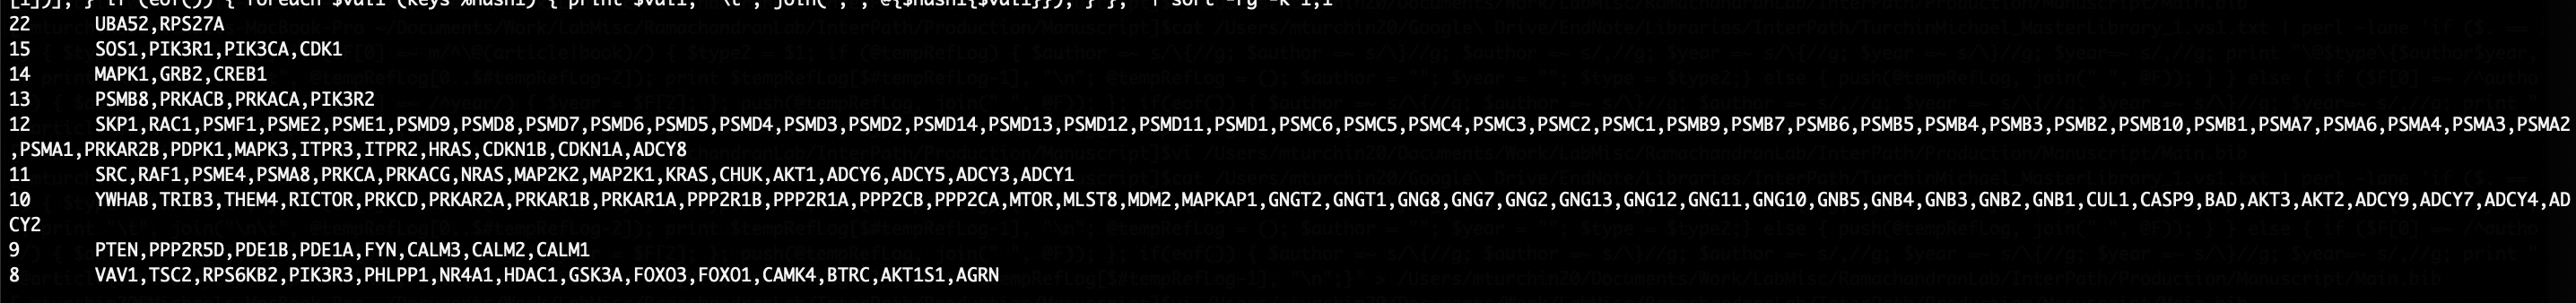
\includegraphics[scale=1]{Images/Supp/InterPath_Supp_Table_TopPathwayGeneCounts.png}
%\caption[TBD]{\textbf{Table of Most Present Genes in Significant MAPIT-R Pathways} \textcolor{red}{this will be a table}}
%\label{InterPath-Supp-Tables-GeneCounts}
%\end{figure}
%\end{landscape}
%\clearpage

\newcounter{CharNumber2}
\setcounter{CharNumber2}{1}
\renewcommand{\thetable}{\arabic{table}\alph{CharNumber2}}
\setlength{\footskip}{3cm}
\begin{landscape}
\begin{table}[ht]
\centering
\hspace*{-1.75cm}
\begin{tabular}{ccl}
  \hline
\textbf{Population} & \textbf{Gene Count} & \textbf{Genes} \\
  \hline
 \textbf{African} & & \\
 & 11 & MAPK3,MAPK1 \\
  & 10 & TNF \\
  &  9 & PRKCB,PLCB4,PLCB3,PLCB2,PLCB1,HRAS \\
  &  8 & RAF1,PRKCG,PRKCA,NRAS,MAP2K1,KRAS,HLA-G,HLA-E,HLA-DRB1,HLA-DRA,HLA-DQB1, \\
  & & HLA-DQA2,HLA-DQA1,HLA-DPB1,HLA-DPA1,HLA-DOB,HLA-DOA,HLA-DMB,HLA-DMA, \\
  & & HLA-C,HLA-B,HLA-A \\
  &  7 & PRKACG,PRKACB,PRKACA,MAP2K2,ITPR1,HLA-F,FAS,CD86,CD80,CD28,CACNA1C,BRAF \\
  &  6 & RAC2,RAC1,PRF1,PIK3R5,PIK3R3,PIK3R2,PIK3R1,PIK3CG,PIK3CD,PIK3CB,PIK3CA,ITPR3, \\ 
  & & ITPR2,IL2,IFNG,GNAQ,FASLG,CD40,CALML6,CALML5,CALML3,CALM3,CALM2,CALM1, \\
  & & CACNA1D,ADCY8,ADCY3,ADCY1 \\
  &  5 & SOS2,SOS1,ROCK2,ROCK1,RHOA,RAC3,PPP3R1,PPP3CC,PPP3CB,PPP3CA,PDGFRA,ITGB7, \\ 
  & & ITGB1,ITGA4,IL10,GZMB,EGFR,EGF,CXCR4,CHP2,CACNA1S,ADCY9,ADCY7,ADCY6, \\
  & & ADCY5,ADCY4,ADCY2,ACTG1,ACTB \\
  \\
  \textbf{Caribbean} & & \\
  & 6 & ITGB1 \\
  \\
  \textbf{Chinese} & & \\
  & 5 & HLA-DRB5,HLA-DRB1,HLA-DRA,HLA-DQB1,HLA-DQA2,HLA-DQA1,HLA-DPB1,HLA-DPA1, \\
  & & HLA-DOB,HLA-DOA,HLA-DMB,HLA-DMA \\
   \hline
\end{tabular}
\caption[TBD]{\textbf{Gene counts across MAPIT-R genome-wide significant KEGG pathways in height, per subgroup}. Caption continued at end of tables.}
\label{InterPath-Supp-Tables-AllPops-TopGeneCounts-KEGG-Height-a}
\end{table}
\clearpage
\addtocounter{table}{-1}
\addtocounter{CharNumber2}{1}

\begin{table}[ht]
\centering
\vspace*{-1.cm}
\hspace*{-1.75cm}
\begin{tabular}{ccl}
  \hline
\textbf{Population} & \textbf{Gene Count} & \textbf{Genes} \\
  \hline
  \textbf{African} & & \\
  & 18 & MAPK3,MAPK1 \\
  & 14 & PIK3CG,PIK3CD,PIK3CB,PIK3CA,HRAS \\
  & 13 & RAF1,PIK3R5,PIK3R3,PIK3R2,PIK3R1,NRAS,MAP2K1,KRAS \\
  & 12 & TNF,PRKCB,MAP2K2 \\
  & 11 & SOS2,SOS1 \\
  & 10 & PRKCG,PRKCA,HLA-DRB1,HLA-DRA,HLA-DQB1,HLA-DQA2,HLA-DQA1,HLA-DPB1,HLA-DPA1, \\
  & & HLA-DOB,HLA-DOA,HLA-DMB,HLA-DMA,GSK3B,GRB2,BRAF \\
  &  9 & TP53,RHOA,RAC1,PLCB4,PLCB3,PLCB2,PLCB1,ITGB1,CCND1,AKT3,AKT2,AKT1 \\
  &  8 & RAC2,PRKACG,PRKACB,PRKACA,PLCG1,ITGA4,IL10,IFNG,HLA-G,HLA-E,HLA-C,HLA-B, \\
  & & HLA-A,EP300,EGFR,CREBBP,CDC42,CD28 \\
  &  7 & PLCG2,IL4,IL2,HLA-F,FAS,EGF,CD86,CD80,CASP9,CAMK2G,CAMK2D,CAMK2B,CAMK2A, \\ 
  & & CALML6,CALML5,CALML3,CALM3,CALM2,CALM1,CACNA1C,ADCY8,ADCY3,ADCY1, \\
  & & ACTG1,ACTB \\
  &  6 & ROCK2,ROCK1,RELA,RAC3,PTK2,PRF1,PPP3R1,PPP3CC,PPP3CB,PPP3CA,PAK1,NFKBIA, \\ 
  & & NFKB1,LAMA2,ITGB7,ITGAV,ITGA6,ITGA3,ITGA2B,ITGA2,IL5,IKBKB,GNAQ,FASLG, \\
  & & CTNNB1,CHP2,CDK4,CD40,CACNA1D,ADCY9,ADCY7,ADCY6,ADCY5,ADCY4,ADCY2 \\
  &  5 & VAV3,VAV2,VAV1,TGFB1,TCF7L2,TCF7L1,TCF7,SHC4,SHC3,SHC2,SHC1,RB1,PTPN6,PTEN, \\ 
  & & PDGFRA,MYC,MDM2,MAPK9,LEF1,JUN,ITPR1,ITGB8,ITGB6,ITGB5,ITGB4,ITGB3,ITGB2, \\ 
  & & ITGA9,ITGA8,ITGA7,ITGA11,ITGA10,ITGA1,IGF1,GZMB,GNAI3,GNAI1,FYN,E2F3,E2F2,E2F1, \\ 
  & & DAG1,CYCS,CXCR4,CDKN1A,CDK6,CASP3,CACNA1S,BAD,ACTN4,ACTN3,ACTN2,ACTN1,ABL1 \\ 
  \\
  \textbf{Chinese} & & \\
  & 7 & HLA-DRB5,HLA-DRB1,HLA-DRA,HLA-DQB1,HLA-DQA2,HLA-DQA1,HLA-DPB1,HLA-DPA1, \\ 
  & & HLA-DOB,HLA-DOA,HLA-DMB,HLA-DMA \\
  &  6 & TNF \\
  &  5 & IFNG,HLA-G,HLA-F,HLA-E,HLA-C,HLA-B,HLA-A,CD86,CD80,CD28 \\
   \hline
\end{tabular}
\caption[TBD]{\textbf{Gene counts across MAPIT-R genome-wide significant KEGG pathways in BMI, per subgroup}}
\label{InterPath-Supp-Tables-AllPops-TopGeneCounts-KEGG-BMI-a}
\end{table}
\clearpage
\addtocounter{table}{-1}
\addtocounter{CharNumber2}{1}

\begin{table}[ht]
\centering
\vspace*{0cm}
\hspace*{-1.75cm}
\begin{tabular}{ccl}
  \hline
\textbf{Population} & \textbf{Gene Count} & \textbf{Genes} \\
  \hline
  \textbf{African} & & \\
   & 8 & MAPK1 \\
    & 7 & PIK3R2,PIK3R1,PIK3CA \\
    & 6 & SOS1,MAPK3,MAP2K2,MAP2K1,GRB2,CREB1,CDK1 \\
    & 5 & UBA52,RPS27A,RAF1,PRKCD,PRKACB,PPP2R5D,PPP2R1B,PPP2R1A,PPP2CB, \\
    & & PPP2CA,ITPR3,ITPR2,ITGB1,HRAS,GNGT2,GNGT1,GNG8,GNG7,GNG2,GNG13, \\ 
    & & GNG12,GNG11,GNG10,GNB5,GNB4,GNB3,GNB2,GNB1 \\
   \hline
\end{tabular}
\caption[TBD]{\textbf{Gene counts across MAPIT-R genome-wide significant REACTOME pathways in height, per subgroup}}
\label{InterPath-Supp-Tables-AllPops-TopGeneCounts-REACTOME-Height-a}
\end{table}
\clearpage
\addtocounter{table}{-1}
\addtocounter{CharNumber2}{1}

\begin{table}[ht]
\centering
\vspace*{-2cm}
\hspace*{-2cm}
\begin{tabular}{ccl}
  \hline
\textbf{Population} & \textbf{Gene Count} & \textbf{Genes} \\
  \hline
  \textbf{African} & & \\
  & 22 & UBA52,RPS27A \\
  & 15 & SOS1,PIK3R1,PIK3CA,CDK1 \\
  & 14 & MAPK1,GRB2,CREB1 \\
  & 13 & PSMB8,PRKACB,PRKACA,PIK3R2 \\
  & 12 & SKP1,RAC1,PSMF1,PSME2,PSME1,PSMD9,PSMD8,PSMD7,PSMD6,PSMD5,PSMD4,PSMD3, \\
  & & PSMD2,PSMD14,PSMD13,PSMD12,PSMD11,PSMD1,PSMC6,PSMC5,PSMC4,PSMC3,PSMC2, \\ 
  & & PSMC1,PSMB9,PSMB7,PSMB6,PSMB5,PSMB4,PSMB3,PSMB2,PSMB10,PSMB1,PSMA7, \\
  & & PSMA6,PSMA4,PSMA3,PSMA2,PSMA1,PRKAR2B,PDPK1,MAPK3,ITPR3,ITPR2,HRAS, \\
  & & CDKN1B,CDKN1A,ADCY8 \\
  & 11 & SRC,RAF1,PSME4,PSMA8,PRKCA,PRKACG,NRAS,MAP2K2,MAP2K1,KRAS,CHUK,AKT1, \\
  & & ADCY6,ADCY5,ADCY3,ADCY1 \\
  & 10 & YWHAB,TRIB3,THEM4,RICTOR,PRKCD,PRKAR2A,PRKAR1B,PRKAR1A,PPP2R1B, \\ 
  & & PPP2R1A,PPP2CB,PPP2CA,MTOR,MLST8,MDM2,MAPKAP1,GNGT2,GNGT1,GNG8,GNG7, \\
  & & GNG2,GNG13,GNG12,GNG11,GNG10,GNB5,GNB4,GNB3,GNB2,GNB1,CUL1,CASP9,BAD,AKT3, \\
  & & AKT2,ADCY9,ADCY7,ADCY4,ADCY2 \\
    & 9 & PTEN,PPP2R5D,PDE1B,PDE1A,FYN,CALM3,CALM2,CALM1 \\
    & 8 & VAV1,TSC2,RPS6KB2,PIK3R3,PHLPP1,NR4A1,HDAC1,GSK3A,FOXO3,FOXO1,CAMK4,BTRC, \\ 
    & & AKT1S1,AGRN \\
    & 7 & RPA3,RPA2,RPA1,RBX1,PRKCG,PRKCE,NCAN,CDK2 \\
    & 6 & TRIO,SHC1,SEH1L,SDC4,SDC3,SDC2,SDC1,RANBP2,PLCG1,PLCB3,PLCB2,PLCB1,PIK3CB, \\ 
    & & ORC5,ORC4,ORC3,ORC2,ORC1,NUP85,NUP43,NUP37,NUP133,NUP107,MYC,MCM8,MCM7, \\
    & & MCM6,MCM5,MCM4,MCM3,MCM2,LCK,KALRN,HSPG2,GPC6,GPC5,GPC2,GPC1,GNAS, \\ 
    & & GNAI2,GNAI1,E2F3,E2F1,CDC6,CDC42,ADAM17 \\  
    & 5 & YES1,WEE1,VCAN,STAT5B,STAT5A,STAT3,STAG1,SMC3,SAA1,RELA,RASGRF2,RASGRF1, \\
    & & RAD21,PTPN6,PSEN2,PSEN1,PRIM2,PRIM1,POLE2,POLE,POLA2,PLA2G4A,PAK2,NCSTN, \\
    & & MNAT1,MCM10,MAPK8,MAPK14,ITGB3BP,IKBKB,HIST4H4,HIST2H2AA3,HIST1H4L, \\
    & & HIST1H4K,HIST1H4J,HIST1H4H,HIST1H4F,HIST1H4E,HIST1H4D,HIST1H4C,HIST1H4B, \\
    & & HIST1H4A,HIST1H2BO,HIST1H2BN,HIST1H2BM,HIST1H2BL,HIST1H2BK,HIST1H2BJ,HIST1H2BI, \\
    & & HIST1H2BH,HIST1H2BG,HIST1H2BF,HIST1H2BE,HIST1H2BD,HIST1H2BC,HIST1H2BB, \\
    & & HIST1H2AJ,HIST1H2AE,HIST1H2AD,HIST1H2AC,HIST1H2AB,HEXB,HEXA,HDAC2,H2AFZ, \\
    & & GXYLT2,GXYLT1,GRP,GCGR,FFAR1,EP300,E2F2,DCN,DBF4,CSPG4,CRK,CREBBP,CHRM3, \\
    & & CDT1,CDK7,CDC7,CDC45,CCNH,BCAN,B4GALT7,B3GAT2,B3GAT1,B3GALT6,ATR,APP, \\ 
    & & APH1B,APH1A,AP2S1,AP2M1,AP2B1,AP2A2,AP2A1 \\
   \hline
\end{tabular}
\caption[TBD]{\textbf{Gene counts across MAPIT-R genome-wide significant REACTOME pathways in BMI, per subgroup}}
\label{InterPath-Supp-Tables-AllPops-TopGeneCounts-REACTOME-BMI-a}
\end{table}
\clearpage
\addtocounter{table}{-1}
\addtocounter{CharNumber2}{1}
\end{landscape}
\renewcommand{\thetable}{\arabic{table}}
\setlength{\footskip}{1cm}

\begin{table} [t!]
  \caption{\textbf{Gene counts across MAPIT-R genome-wide significant pathways, per subgroup}. The tables show the lists of genes that appear most frequently across the pathways that were MAPIT-R genome-wide significant in the following phenotype and pathway database combinations: (a) KEGG height, (b) KEGG BMI, (c) REACTOME height, and (d) REACTOME BMI. The first columns list the UKB subgroups, the second columns list the number of times the given genes appeared in the set of genome-wide significant pathways for that subgroup, pathway database, and phenotype combination, and the third columns list the actual gene names for each of these numbers of gene counts.}
\label{InterPath-Supp-Tables-AllPops-TopGeneCounts-Caption}
\end{table}
\clearpage

\setlength{\footskip}{2cm}
\begin{table}[ht]
\centering
\begin{tabular}{ccccc}
  \hline
  \textbf{Database} & \textbf{Gene} & \textbf{No Restriction} & \textbf{Restricted} & \textbf{-$\log_{10}$($p$-Value)} \\
  & & \textbf{$p$-Value} & \textbf{$p$-Value} & \textbf{Difference} \\
  \hline
  \textbf{KEGG:} & & & & \\
  & CDKN2A & 1.248E-01 & 7.974E-03 & 1.194 \\
  & CCNB2 & 2.795E-01 & 1.876E-02 & 1.173 \\
  & CCNB1 & 2.795E-01 & 1.876E-02 & 1.173 \\
  & PTEN & 5.340E-02 & 4.186E-03 & 1.106 \\
  & GADD45G & 6.710E-02 & 6.559E-03 & 1.010 \\
  & GADD45B & 6.710E-02 & 6.559E-03 & 1.010 \\
  & GADD45A & 6.710E-02 & 6.559E-03 & 1.010 \\
  & CHEK2 & 6.710E-02 & 6.559E-03 & 1.010 \\
  & CHEK1 & 6.710E-02 & 6.559E-03 & 1.010 \\
  & ATR & 6.710E-02 & 6.559E-03 & 1.010 \\
  \\
  \textbf{REACTOME:} & & & & \\ 
  & SMC3 & 1.456E-05 & 5.589E-09 & 3.416 \\
  & PSM* & 5.304E-04 & 4.464E-06 & 2.075 \\
  & (Cluster) & & & \\ 
  & FBXW11 & 7.902E-02 & 1.956E-03 & 1.606 \\
  & NFKBIE & 2.702E-02 & 1.956E-03 & 1.140 \\
  & PRKCB & 2.204E-01 & 1.797E-02 & 1.089 \\
  & MALT1 & 7.902E-02 & 1.109E-02 & 0.853 \\
  & LOC646626 & 7.902E-02 & 1.109E-02 & 0.853 \\
  & CARD11 & 7.902E-02 & 1.109E-02 & 0.8.53 \\
  & BCL10 & 7.902E-02 & 1.109E-02 & 0.8.53 \\
  & ATR & 8.004E-03 & 1.261E-03 & 0.8.02 \\
   \hline
\end{tabular}
\caption[TBD]{\textbf{Size restricted examples of gene count hypergeometric enrichment tests}. The table shows the top examples of genes that became more significant in the hypergeometric enrichment analyses after the size restriction step in both pathway databases. Results are only shown for BMI since the majority of genome-wide significant pathways in height were lost from the size restriction step alone. The first column lists the pathway database, the second column lists the genes, the third column lists the original, unrestricted hypergeometric enrichment $p$-value, the fourth column lists the new, size-restricted hypergeometric enrichment $p$-value, and the fifth column lists the -$\log_{10}$ $p$-value difference between the third and fourth column. The top 10 genes sorted by the fifth column are shown for each database. For a plot of results from every gene analyzed in both databases, see Supplementary Figure \ref{InterPath-Supp-Figure-Hypergeometric-RestrictedComps-African-BMI}). Note that a single entry in the REACTOME results is included to represent the PSM* gene family cluster to preserve space.}
\label{InterPath-Supp-Table-Hypergeometric-RestrictedComps-African-BMI-TopExamples}
\end{table}
\clearpage
\setlength{\footskip}{1cm}

\begin{landscape}
\begin{table}[ht]
\centering
\hspace*{-1.5cm}
\begin{tabular}{ccccccc}
  \hline
  \textbf{Gene} & \textbf{Pathway SNP} & \textbf{Gene Count in} & \textbf{Total Count of} & \textbf{Gene Count in} & \textbf{Total Count of} & \textbf{Hypergeometric} \\
   & \textbf{Count Limit} & \textbf{Top Pathways} & \textbf{Top Pathways} & \textbf{All Pathways} & \textbf{All Pathways} & \textbf{$p$-Value} \\
  \hline
 \textbf{UBA52} & & & & & & \\
 & No Limit & 22 & 65 & 106 & 658 & 1.537E-4 \\
 & $<$ 1000 SNPs & 10 & 26 & 84 & 577 & 1.855E-3 \\
\\
 \textbf{PSM*} & & & & & & \\
 & No Limit & 12 & 65 & 44 & 658 & 5.304E-4 \\
 & $<$ 1000 SNPs & 9 & 26 & 34 & 577 & 4.464E-6 \\
   \hline
\end{tabular}
\caption[TBD]{\textbf{MAPIT-R Genome-Wide Significant Pathway Gene Counts: Hypergeometric Enrichment Examples}. Caption continued on next page.}
\label{InterPath-Supp-Tables-AllPops-TopGeneCount-HypergeometricTests}
\end{table}
\end{landscape}
\clearpage

\addtocounter{table}{-1}
\begin{table} [t!]
  \caption{\textbf{PSM* and UBA52 gene count enrichment test examples, size restriction and no restriction}. The table shows examples and results of running the hypergeometric test for enrichment on two different genes in two different study designs. In all cases a gene is tested for being significantly more frequent among the set of MAPIT-R genome-wide significant pathways than among the background distribution of pathways in the original database. Two study designs were employed for these tests, either (a) using all pathways present in the given databases or (b) using only pathways that contained less than or equal to 1,000 SNPs. The first column lists the gene or gene family being tested. The second column lists which of the two aforementioned study designs was used. Columns three through six list the different count values used in the hypergeometric test: the third column lists the number of times a gene is present among the genome-wide significant list of pathways, the fourth column lists the total number of pathways that were genome-wide significant, the fifth column lists the number of times a gene is present among all the pathways in the given database, and the sixth column lists the total number of pathways in the given database. The seventh column is the hypergeometric $p$-value associated with columns three through six. Note that the vast majority of proteasome genes included in our analysis had the same number of gene counts across each hypergeometric category, hence why \textbf{PSM*} was used to represent them as a whole.}
\label{InterPath-Supp-Tables-AllPops-TopGeneCount-HypergeometricTests-Caption}
\end{table}
\clearpage

%\begin{landscape}
%\setlength{\footskip}{2cm}
%\begin{table}[ht]
%\centering
%\begin{tabular}{lrrr}
%  \hline
%\textbf{Pathway} & \textbf{Genes} & \textbf{SNPs} & %\textbf{$p$-Value} \\ 
%  \hline
%REACTOME\_M\_G1\_TRANSITION & 73 & 458 & 3.191E-06 \\ 
%  REACTOME\_CELL\_CYCLE\_CHECKPOINTS & 105 & 670 & 5.781E-06 \\ 
%  REACTOME\_HOST\_INTERACTIONS\_OF\_HIV\_FACTORS & 112 & 963 & 7.521E-06 \\ 
%  REACTOME\_DOWNSTREAM\_SIGNALING\_EVENTS\_OF\_ & & & \\ 
%  \qquad B\_CELL\_RECEPTOR\_BCR & 89 & 745 & 1.195E-05 \\
%  REACTOME\_REGULATION\_OF\_APOPTOSIS & 52 & 564 & 1.218E-05 \\ 
%  REACTOME\_MITOTIC\_G1\_G1\_S\_PHASES & 121 & 747 & 1.453E-05 \\ 
%  REACTOME\_ACTIVATION\_OF\_NF\_KAPPAB\_IN\_B\_CELLS & 59 & 465 & 1.861E-05 \\ 
%  REACTOME\_ASSEMBLY\_OF\_THE\_PRE\_REPLICATIVE\_COMPLEX & 60 & 331 & 3.293E-05 \\ 
%  REACTOME\_ANTIGEN\_PROCESSING\_CROSS\_PRESENTATION & 68 & 850 & 3.956E-05 \\ 
%   \hline
%\end{tabular}
%  \caption{\textbf{Size-restricted pathways that contain the PSM* cluster of genes}. Caption continued on next page.}
%\label{InterPath-Supp-Tables-AllPops-TopGeneCount-SizeRestricted-Proteasome}
%\end{table}
%\clearpage
%\end{landscape}
%\setlength{\footskip}{1cm}

%\addtocounter{table}{-1}
%\begin{table} [t!]
%  \caption{\textbf{Size-restricted pathways that contain the PSM* cluster of genes}. The table shows the MAPIT-R genome-wide significant REACTOME pathways for BMI in the African subgroup that both have SNP sizes less than 1,000 and also contain the set of proteasome genes being investigated (\textit{PSMA}*, \textit{PSMB}*, \textit{PSMC}*, \textit{PSMD}*, and \textit{PSME*}). The first column shows the REACTOME pathway names, the second column shows the number of genes that were included in the MAPIT-R analysis, the third column show the number of SNPs that were included in the MAPIT-R analysis, and the fourth column shows the MAPIT-R $p$-value.}
%\label{InterPath-Supp-Tables-AllPops-TopGeneCount-SizeRestricted-Proteasome-Caption}
%\end{table}
%\clearpage

%\begin{figure}[htbp]
%\centering
%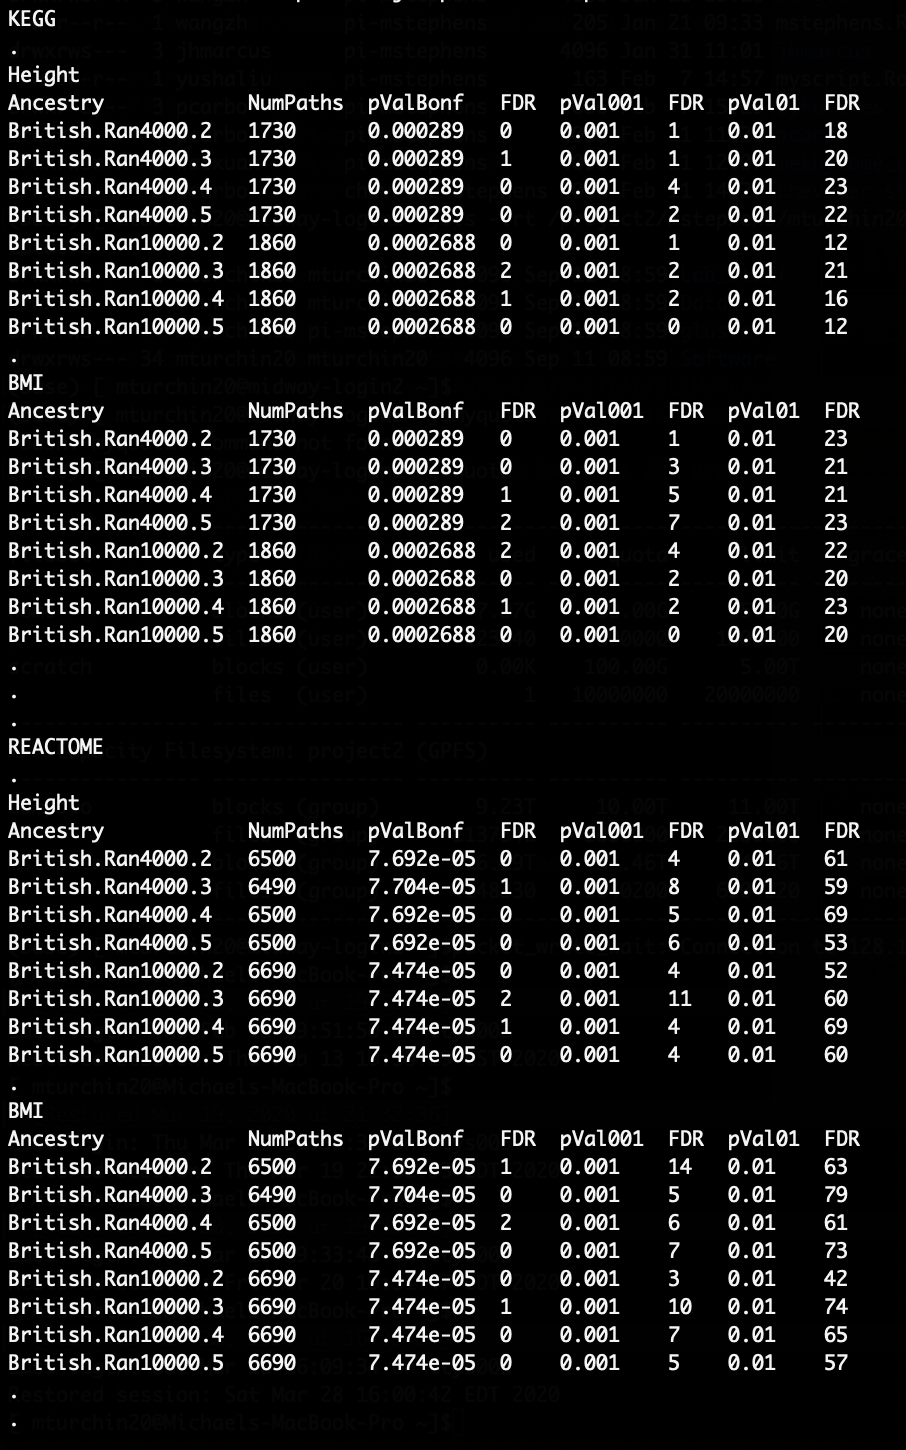
\includegraphics[scale=1.5]{Images/Supp/InterPath_Supp_Figure_FDRs_BritReps_vs1.png}
%\caption[TBD]{\textbf{TBD}. }
%\label{InterPath-Supp-Figure-BritReps-FDRs}
%\end{figure}
%\clearpage

\setlength{\footskip}{4cm}
\begin{landscape}
\begin{table}[ht]
\vspace*{-1.25cm}
\centering
\hspace*{-3.25cm}
\begin{tabular}{ccccccccccc}
  \hline
\textbf{Population} & \textbf{Pathway} & \textbf{Bonferroni} & \textbf{Bonferroni} & \textbf{Bonferroni} & \textbf{0.001} & \textbf{0.001} & \textbf{0.001} & \textbf{0.01} & \textbf{0.01} & \textbf{0.01} \\
 & \textbf{Counts} & \textbf{Threshold} & \textbf{Counts} & \textbf{FDR} & \textbf{Threshold} & \textbf{Counts} & \textbf{FDR} & \textbf{Threshold} & \textbf{Counts} & \textbf{FDR} \\ 
  \hline
\textbf{KEGG Height:} & & & & & & & & & \\
British.Ran4000 & 1730 & 2.890E-04 & 0 & 0.000 & 0.001 & 0 & 0.000 & 0.010 & 13 & 0.751 \\
  British.Ran4000.2 & 1730 & 2.890E-04 & 0 & 0.000 & 0.001 & 1 & 0.058 & 0.010 & 18 & 1.040 \\
  British.Ran4000.3 & 1730 & 2.890E-04 & 1 & 0.058 & 0.001 & 1 & 0.058 & 0.010 & 20 & 1.156 \\
  British.Ran4000.4 & 1730 & 2.890E-04 & 0 & 0.000 & 0.001 & 4 & 0.231 & 0.010 & 23 & 1.329 \\
  British.Ran4000.5 & 1730 & 2.890E-04 & 0 & 0.000 & 0.001 & 2 & 0.116 & 0.010 & 22 & 1.272 \\
  British.Ran10000.1 & 1860 & 2.688E-04 & 0 & 0.000 & 0.001 & 1 & 0.054 & 0.010 & 26 & 1.398 \\
  British.Ran10000.2 & 1860 & 2.688E-04 & 0 & 0.000 & 0.001 & 1 & 0.054 & 0.010 & 12 & 0.645 \\
  British.Ran10000.3 & 1860 & 2.688E-04 & 2 & 0.108 & 0.001 & 2 & 0.108 & 0.010 & 21 & 1.129 \\
  British.Ran10000.4 & 1860 & 2.688E-04 & 1 & 0.054 & 0.001 & 2 & 0.108 & 0.010 & 16 & 0.860 \\
  British.Ran10000.5 & 1860 & 2.688E-04 & 0 & 0.000 & 0.001 & 0 & 0.000 & 0.010 & 12 & 0.645 \\
  \\
  \textbf{KEGG BMI:} & & & & & & & & & \\
British.Ran4000 & 1730 & 2.890E-04 & 1 & 0.058 & 0.001 & 2 & 0.116 & 0.010 & 14 & 0.809 \\
  British.Ran4000.2 & 1730 & 2.890E-04 & 0 & 0.000 & 0.001 & 1 & 0.058 & 0.010 & 23 & 1.329 \\
  British.Ran4000.3 & 1730 & 2.890E-04 & 0 & 0.000 & 0.001 & 3 & 0.173 & 0.010 & 21 & 1.214 \\
  British.Ran4000.4 & 1730 & 2.890E-04 & 1 & 0.058 & 0.001 & 5 & 0.289 & 0.010 & 21 & 1.214 \\
  British.Ran4000.5 & 1730 & 2.890E-04 & 2 & 0.116 & 0.001 & 7 & 0.405 & 0.010 & 23 & 1.329 \\
  British.Ran10000.1 & 1860 & 2.688E-04 & 0 & 0.000 & 0.001 & 1 & 0.054 & 0.010 & 25 & 1.344 \\
  British.Ran10000.2 & 1860 & 2.688E-04 & 2 & 0.108 & 0.001 & 4 & 0.215 & 0.010 & 22 & 1.183 \\
  British.Ran10000.3 & 1860 & 2.688E-04 & 0 & 0.000 & 0.001 & 2 & 0.108 & 0.010 & 20 & 1.075 \\
  British.Ran10000.4 & 1860 & 2.688E-04 & 1 & 0.054 & 0.001 & 2 & 0.108 & 0.010 & 23 & 1.237 \\
  British.Ran10000.5 & 1860 & 2.688E-04 & 0 & 0.000 & 0.001 & 0 & 0.000 & 0.010 & 20 & 1.075 \\
   \hline
\end{tabular}
\caption[TBD]{\textbf{MAPIT-R false discovery rates at different significance thresholds, per British replicate}. Caption continued at end of tables.}
\label{InterPath-Supp-Tables-BritReps-FDRs-pt1}
\end{table}
\end{landscape}
\clearpage
\setlength{\footskip}{1cm}
\addtocounter{table}{-1}

\setlength{\footskip}{4cm}
\renewcommand{\thetable}{\arabic{table}}
\begin{landscape}
\begin{table}[ht]
\vspace*{-1.25cm}
\centering
\hspace*{-3.5cm}
\begin{tabular}{ccccccccccc}
  \hline
\textbf{Population} & \textbf{Pathway} & \textbf{Bonferroni} & \textbf{Bonferroni} & \textbf{Bonferroni} & \textbf{0.001} & \textbf{0.001} & \textbf{0.001} & \textbf{0.01} & \textbf{0.01} & \textbf{0.01} \\
 & \textbf{Counts} & \textbf{Threshold} & \textbf{Counts} & \textbf{FDR} & \textbf{Threshold} & \textbf{Counts} & \textbf{FDR} & \textbf{Threshold} & \textbf{Counts} & \textbf{FDR} \\ 
  \hline
  \textbf{REACTOME Height:} & & & & & & & & & \\
British.Ran4000 & 6500 & 7.692E-05 & 0 & 0.000 & 0.001 & 9 & 0.138 & 0.010 & 69 & 1.062 \\
  British.Ran4000.2 & 6500 & 7.692E-05 & 0 & 0.000 & 0.001 & 4 & 0.062 & 0.010 & 61 & 0.938 \\
  British.Ran4000.3 & 6490 & 7.704E-05 & 1 & 0.015 & 0.001 & 8 & 0.123 & 0.010 & 59 & 0.909 \\
  British.Ran4000.4 & 6500 & 7.692E-05 & 0 & 0.000 & 0.001 & 5 & 0.077 & 0.010 & 69 & 1.062 \\
  British.Ran4000.5 & 6500 & 7.692E-05 & 0 & 0.000 & 0.001 & 6 & 0.092 & 0.010 & 53 & 0.815 \\
   British.Ran10000.1 & 6690 & 7.474E-05 & 0 & 0.000 & 0.001 & 4 & 0.060 & 0.010 & 55 & 0.822 \\
  British.Ran10000.2 & 6690 & 7.474E-05 & 0 & 0.000 & 0.001 & 4 & 0.060 & 0.010 & 52 & 0.777 \\
  British.Ran10000.3 & 6690 & 7.474E-05 & 2 & 0.030 & 0.001 & 11 & 0.164 & 0.010 & 60 & 0.897 \\
  British.Ran10000.4 & 6690 & 7.474E-05 & 1 & 0.015 & 0.001 & 4 & 0.060 & 0.010 & 69 & 1.031 \\
  British.Ran10000.5 & 6690 & 7.474E-05 & 0 & 0.000 & 0.001 & 4 & 0.060 & 0.010 & 60 & 0.897 \\

  \\
  \textbf{REACTOME BMI:} & & & & & & & & & \\
British.Ran4000 & 6490 & 7.704E-05 & 1 & 0.015 & 0.001 & 4 & 0.062 & 0.010 & 52 & 0.801 \\
  British.Ran4000.2 & 6500 & 7.692E-05 & 1 & 0.015 & 0.001 & 14 & 0.215 & 0.010 & 63 & 0.969 \\
  British.Ran4000.3 & 6490 & 7.704E-05 & 0 & 0.000 & 0.001 & 5 & 0.077 & 0.010 & 79 & 1.217 \\
  British.Ran4000.4 & 6500 & 7.692E-05 & 2 & 0.031 & 0.001 & 6 & 0.092 & 0.010 & 61 & 0.938 \\
  British.Ran4000.5 & 6500 & 7.692E-05 & 0 & 0.000 & 0.001 & 7 & 0.108 & 0.010 & 73 & 1.123 \\
  British.Ran10000.1 & 6690 & 7.474E-05 & 2 & 0.030 & 0.001 & 10 & 0.149 & 0.010 & 73 & 1.091 \\
  British.Ran10000.2 & 6690 & 7.474E-05 & 0 & 0.000 & 0.001 & 3 & 0.045 & 0.010 & 42 & 0.628 \\
  British.Ran10000.3 & 6690 & 7.474E-05 & 1 & 0.015 & 0.001 & 10 & 0.149 & 0.010 & 74 & 1.106 \\
  British.Ran10000.4 & 6690 & 7.474E-05 & 0 & 0.000 & 0.001 & 7 & 0.105 & 0.010 & 65 & 0.972 \\
  British.Ran10000.5 & 6690 & 7.474E-05 & 0 & 0.000 & 0.001 & 5 & 0.075 & 0.010 & 57 & 0.852 \\
   \hline
\end{tabular}
\caption[TBD]{\textbf{MAPIT-R false discovery rates at different significance thresholds, per British replicate}. Continued.}
\label{InterPath-Supp-Tables-BritReps-FDRs-pt2}
\end{table}
\end{landscape}
\clearpage
\setlength{\footskip}{1cm}

\addtocounter{table}{-1}
\begin{table} [t!]
  \caption{\textbf{MAPIT-R false discovery rates at different significance thresholds, per British replicate}. The tables show for various significance thresholds the false discovery rates observed from MAPIT-R when run on ten rounds of phenotype permutations for each British replicate subsample and pathway database. The first column lists the pathway database, phenotype, and British replicate subsample combinations. The second column lists the total number of pathways that were tested across each of the ten phenotype permutations. The third column shows the $p$-value threshold associated with using the Bonferroni method of correction, also known as the `genome-wide significant' threshold. The fourth column shows the number of pathways across all ten phenotype permutation rounds that crossed this Bonferroni threshold. The fifth column shows the associated FDR associated with the fourth column. And the remaining six columns show the same setup as columns three to five but with a $p$-value threshold of either 0.001 or 0.01.}
\label{InterPath-Supp-Tables-BritReps-FDRs-Caption}
\end{table}
\clearpage

\nolinenumbers

\begingroup
\bibliographystyle{apalike}
\setstretch{1.0}
\bibliography{Main}
\endgroup














\iffalse

SCRAP








not only is there an example of a gene family having a strong impact on the pathway-level signal for marginal epistasis, subunit  

for 






Each component of the proteasome is encoded by one of the aforementioned gene family subunits, producing a situation to possibly further refine the original, pathway-level signals for marginal epistasis. Since each subunit family has a distinct set of SNPs mapping to them, we can incrementally remove 

For the purposes of our investigation of marginal epistasis, the prot


The proteasome itself is made up of a core of four stacked rings (proteins from the subunits \textit{PSMA}* and \textit{PSMB}*) that need to be broken down are tagged by ubiquitin and are eventually directed to the proteasome, wh

ich  Each of these subunits also correspond to specific structural components of the proteasome itself, offering a chance to further explore the 


And most of these genes fall in the same family, as components of the various proteins that make up the proteasome. 

One set of genes corresponds to the different substructures of the proteasome (), and the second set is a single gene, XXX, which encodes the protein ubiquitin. In fact, both the proteasome and ubiquitin together form ubiquitin-proteasome system (UPS).



And in fact both sets of genes correspond to the same biological process, the ubiquitin-proteasome system (UPS).

The first set of The first set is a cluster of genes that all correspond to different parts of the proteasome







though  
This is in spite of alternative non-linear approaches such as incorporatin

. Despite 




Genome-wide association (GWA) studies have identified thousands of significant genetic associations in humans across a number of complex traits. However, the vast majority of these studies use datasets of predominantly European ancestry. This discrepancy is a persistent, known issue, however the body of work showing the benefits of diverse genomic datasets to additive complex trait genetics only continues to grow, including more ancestry-specific estimates of effect sizes and increased discoveries of associated, putative causal variants.\footnote{\red{SR: I'm not sure this sentence is doing much for you. It's also a bit awkwardly phrased and hard to parse - should be shorter and more direct.}} Here, we explore a form of non-additive trait architecture, epistasis, to see if there are similar insights that can be gained in complex traits when analyzing a particularly diverse dataset. 

To increase our power to detect epistasis, we create a new method to detect pathway-level marginal epistasis (MAPIT-R), and apply this method to a diverse group of ancestry subgroups within the UK BioBank (UKB) dataset. We analyze height and BMI with the KEGG and REACTOME databases and find 245 pathways with statistically significant signals of marginal epistasis. We find that 67\% of these results are found in an African subgroup of the UKB data. We find that BMI consistently produces stronger signals of pathway-level marginal epistasis than height. We find that the proteasome is enriched for signals of marginal epistasis and show how region-based tests such as MAPIT-R can be used to further localize association signals. And we investigate the relationship between within-subgroup genetic variation and its impact on the ability to detect marginal epistasis. 














Genome-wide association (GWA) studies are a powerful tool for identifying statistical associations between genetic variation and complex traits, and have identified over 24,000 statistically significant such associations in humans alone \citep{Buniello2019}. However, it is also well-known that GWA studies and related research directions have been incredibly focused on populations of European ancestry\red{, with non-European ancestry samples constituting at most 20\% of analyzed samples in the GWAS Catalog?} \citep{Need2009,Popejoy2016,Gurdasani2019,Martin2019,Sirugo2019}.

This lack of diverse representation \red{persists despite} the numerous ways incorporating non-European\footnote{\red{SR: might be better to just say ``diverse''}} ancestries benefits genomic analyses: for example, imputation performance \citep{Huang2009,Howie2011,Das2018,Kowalski2019}, and polygenic risk score analyses \citep{Martin2017a,Duncan2019,Kerminen2019,Rosenberg2019,Marnetto2020,Mostafavi2020}. In GWA and eQTL studies, investigating more diverse sets of human ancestries can lead\footnote{\red{SR: why not ``leads to" instead of ``can lead to"}} to more accurate effect size estimates and greater numbers of novel associations \citep{Dumitrescu2011,Stranger2012,Carlson2013,Bien2019,Mogil2018,Gurdasani2019,Kuchenbaecker2019,Wojcik2019,Zhong2019}. And further for association study frameworks in general, properly accounting for population structure can limit false positives and increase power to detect associations \citep{Kang2010,Price2010,Zhou2012,Sul2018}.\footnote{\red{SR: not sure how this sentence helps with your argument....structure is usually controlled for, right?}} This last phenomenon is of particular importance as biobank-size datasets only continue to expand; finescale latent population structure is still an ongoing confounder in human genomic analyses \citep{Berg2019,Sohail2019,Lawson2020}, and growing databases may lead to increased exposure of such latent structures \citep{Haworth2019,Dai2020,Sakaue2020,Lawson2020}. 

The question then is why this dataset ancestry representation problem still persists. Structural issues, such as biases in funding allocations and resource availability, are certainly a major contributor. Another contributor may be a continued under appreciation of what investigating non-European populations can provide to genomic analyses. Here, we aim to show once again the profound, if not essential, benefit non-European populations provide in terms of novel insight into human complex trait genetic architecture.\footnote{\red{SR: I would cut this whole paragraph; I appreciate the points but they have been made elsewhere.}}

To accomplish this, we followed past examples of how incorporating diverse collections of human ancestries into GWA, eQTL, and PRS frameworks lead to novel insights into complex trait genetic architecture, and we investigated the potential benefits of incorporating a diverse dataset into frameworks for studying genetic epistasis.\footnote{\red{SR: I would make this sentence start more with ``Our objective here'' and describe that the goal is to detect epistasis at biologically intepretable scales and then to incorporate diverse datasets into such analyses. I think the first sentence you wrote is more of a discussion point. I don't think we should motivate this in this way but rather point out in the Discussion that other studies have taken this approach.}} Epistasis is a well-established phenomenon in a number of model organisms \citep{Lehner2006,Rowe2008,Shao2008,Flint2009,Costanzo2010,He2010,Jarvis2011,Pettersson2011,Bloom2013,Monnahan2015}, and has been suggested as a major \red{driver?} of both complex trait genetic architecture and evolution \citep{Carlborg2004,Carlborg2006,Martin2007,Phillips2008,Moore2009,Jones2014,Mackay2014}. However, there remains skepticism regarding the extent to which epistasis has \red{affected} human populations \citep{Hill2008,Crow2010,Aschard2012,Wood2014,Yang2015}. Recent methodological advances have shown increasing evidence for epistasis in humans \citep{Verma2016,Crawford2017a,Fang2019,Runcie2019}, but most of these efforts have been conducted in European ancestry populations. It is unclear what novel insight a diverse set of non-European populations might provide in epistasis, especially in light of the aforementioned results that additive architecture\footnote{\red{SR: this is the first time you have referred to additive architecture - you should define/refer to GWA effects also}} varies across human populations as well \citep{Dumitrescu2011,Carlson2013,Kuchenbaecker2019,Wojcik2019}.

In this study, we present \red{MAPIT-R}, a new methodological framework for analyzing marginal epistasis on the \red{region and/or?} pathway level. We analyze epistasis in height and body mass index (BMI) at multiple genomic \red{scales} across six different human ancestry subgroups present in the UK BioBank (UKB) \citep{Sudlow2015} dataset, and find that an African ancestry UKB subgroup produces many more significant epistatic pathways than any other UKB ancestry subgroup (165 of 245 total significant pathways \red{how many subgroups analyed?}). \red{You need to define what a significant hit is - a pathway with a large marginal epistatic signal? Marginal epistasis has not been identified, and there's no mention of why one might want to look at pathways? I would think you would want to highlight some GWA enrichment analyses like RSS and gene-e} We find pathways related to cellular signaling and the immune system are often represented among our significant hits, and evidence that the proteasome may be particularly enriched for epistatic interactions.\footnote{\red{SR: I think this sentence, related to my last comment, should start with something like "Our significant hits for epistastic interactions include pathways realted to cellualar signaling...." is this in both traits?}} We find that BMI on average produces stronger signals of pathway-level marginal epistasis than height, in line with previous results suggesting BMI may be more influenced by non-additive factors than height \citep{Elks2012,Visscher2012}. And lastly we find that differences between ancestries are unlikely to be due to large, broadscale patterns of genetic variation.  




Epistasis is a well-established phenomenon in a number of model organisms \citep{Lehner2006,Rowe2008,Shao2008,Flint2009,Costanzo2010,He2010,Jarvis2011,Pettersson2011,Bloom2013,Monnahan2015}, and has been suggested as a major \red{driver?} of both complex trait genetic architecture and evolution \citep{Carlborg2004,Carlborg2006,Martin2007,Phillips2008,Moore2009,Jones2014,Mackay2014}. However, there remains skepticism regarding the extent to which epistasis has \red{affected} human populations \citep{Hill2008,Crow2010,Aschard2012,Wood2014,Yang2015}. Recent methodological advances have shown increasing evidence for epistasis in humans \citep{Verma2016,Crawford2017a,Fang2019,Runcie2019},











by restricting the size of the pathways analyzed, this aims t 

Identifying genes that are enriched among our results may help further focus  






To test whether any genes were significantly enriched across our top pathways, we used a hypergeometric test for enrichment to compare the number of times a gene appears among our significant pathways against the number of times that gene appears in the full distribution of pathways in either the KEGG or REACTOME databases. 

Supplementary Tables \ref{InterPath-Supp-Tables-AllPops-TopGeneCounts-KEGG-Height-a}\textcolor{blue}{-d} shows the various genes present across our significant pathways at different levels of counts, and Supplementary Figure \ref{InterPath-Supp-Figure-Hypergeometric-QQPlots-African} shows the QQ-plots of our hypergeometric enrichment results across these genes. What immediately stands out is the abundance of `significant' $p$-values we find. For example, using the conservative Bonferroni cutoff of $2.082\times10^{-5}$ (.05 / 2401 genes), we would identify 45 genes as being significantly enriched in the REACTOME BMI analysis. However, one major assumption underlying this test is that each pathway is independent from one another, and we know this to not be the case. In fact this assumption is being violated in two ways in regards to the distribution of pathways we are analyzing. 

First, we know that many pathways overlap one another in terms of gene content, and that this particular set of relationships is not easily deconstructed. Second, we also know that the hypothesis underlying our approach is that more SNPs should be correlated to greater levels of significance, and this is indeed what we observe in the results (Supplementary Figure \ref{InterPath-Supp-Figure-pValsVsNumSNPs}); across both phenotypes in both pathway databases, we observe significant relationships between MAPIT-R -$\log_{10}$ $p$-values and the number of SNPs present in an analyzed pathway. This is encouraging in that it supports our initial intuition, but it does lead to significant pathways being more likely to have many SNPs and genes. Therefore when we observe a gene as significantly enriched, it may be possible that the locus just happens to be present in many pathways due to the nature of its function, such as being a `housekeeping' gene. In this case, the enrichment may be less a reflection of our biological interest (genes enriched for epistatic interactions) and more a reflection of the quality of the pathway databases (larger pathways have more similar gene content than smaller pathways do).

The second of these two situations is what we tried to resolve first. If we are concerned about a relationship between larger pathways and inflated hypergeometric $p$-values, then one possible approach might be to restrict the size of the pathways analyzed. Instead of looking at enrichment among all pathways, we can instead look at enrichment only among pathways that have under a certain number of SNPs. And indeed, by restricting the number of SNPs present in a pathway to 1,000 or less, we see a major drop off in the number of significant pathways remaining (29 to 2 for KEGG height, 47 to 11 for KEGG BMI, 24 to 0 for REACTOME height, and 65 to 26 for REACTOME BMI); this, by extension, also produces a large drop in the genes that are present across these pathways as well as their associated hypergeometric $p$-values (Supplementary Figure \ref{InterPath-Supp-Figure-Hypergeometric-RestrictedComps-African-BMI} and Supplementary Table \ref{InterPath-Supp-Table-Hypergeometric-RestrictedComps-African-BMI-TopExamples}). Interestingly however, we find one gene family that has had the opposite result -- multiple proteasome subunit genes (\textit{PSMA}*, \textit{PSMB}*, \textit{PSMC}*, \textit{PSMD}*, and \textit{PSME*}) now produce more significant hypergeometric $p$-values upon this restriction to pathways with smaller SNP counts (Supplementary Table \ref{InterPath-Supp-Tables-AllPops-TopGeneCount-HypergeometricTests}). 

The proteasome is one half of the ubiquitin-proteasome system (UPS), a critical process for proper protein degradation and cell homeostasis \citep{Voges1999,Livneh2016,Collins2017}. And the genes highlighted in this size-restricted analysis represent both the core (20S) and regulatory cap (19S or 11S) subunits of the 26S proteasome, the main variant found within the cytosol of mammalian cells. Looking at the size-restricted pathways these genes are present in, we see multiple pathways related to cell-cycle regulation and, once again, the immune system (Supplementary Table \ref{InterPath-Supp-Tables-AllPops-TopGeneCount-SizeRestricted-Proteasome}). This new, first, category makes sense since protein levels (and therefore their regulation and degradation) are a key component of determining when cells progress through various cycle checkpoints. Encouragingly, these pathways also contain a range of SNP sizes, including multiple pathways with less than 600 SNPs -- this suggests that the results are not simply the product of finding pathways with the next largest set of allowable SNP sizes, but are instead being driven by other factors, such as the underlying biology. More work will be needed to investigate whether these particular results are unique to BMI or are representative of a broadly important protein complex for many phenotypes. But overall these results suggest the proteasome is a prime candidate as a protein complex that is significantly enriched for marginal epistatic interactions.  

%To further look into these proteasome genes, we...




The proteasome is one half of the ubiquitin-proteasome system (UPS), a critical process for proper protein degradation and cell homeostasis \citep{Voges1999,Livneh2016,Collins2017}. And the genes highlighted in this size-restricted analysis represent both the core (20S) and regulatory cap (19S or 11S) subunits of the 26S proteasome, the main variant found within the cytosol of mammalian cells. Looking at the size-restricted pathways these genes are present in, we see multiple pathways related to cell-cycle regulation and, once again, the immune system (Supplementary Table \ref{InterPath-Supp-Tables-AllPops-TopGeneCount-SizeRestricted-Proteasome}).


family that has had the opposite result -- multiple proteasome subunit genes (\textit{PSMA}*, \textit{PSMB}*, \textit{PSMC}*, \textit{PSMD}*, and \textit{PSME*}) now produce more significant hypergeometric $p$-values upon this restriction to pathways with smaller SNP counts (Supplementary Table \ref{InterPath-Supp-Tables-AllPops-TopGeneCount-HypergeometricTests}). 

The proteasome is one half of the ubiquitin-proteasome system (UPS), a critical process for proper protein degradation and cell homeostasis \citep{Voges1999,Livneh2016,Collins2017}. And the genes highlighted in this size-restricted analysis represent both the core (20S) and regulatory cap (19S or 11S) subunits of the 26S proteasome, the main variant found within the cytosol of mammalian cells. Looking at the size-restricted pathways these genes are present in, we see multiple pathways related to cell-cycle regulation and, once again, the immune system (Supplementary Table \ref{InterPath-Supp-Tables-AllPops-TopGeneCount-SizeRestricted-Proteasome}). This new, first, category makes sense since protein levels (and therefore their regulation and degradation) are a key component of determining when cells progress through various cycle checkpoints. Encouragingly, these pathways also contain a range of SNP sizes, including multiple pathways with less than 600 SNPs -- this suggests that the results are not simply the product of finding pathways with the next largest set of allowable SNP sizes, but are instead being driven by other factors, such as the underlying biology. More work will be needed to investigate whether these particular results are unique to BMI or are representative of a broadly important protein complex for many phenotypes. But overall these results suggest the proteasome is a prime candidate as a protein complex that is significantly enriched for marginal epistatic interactions.  



make the removal of  such that particular subsets of the genome, like those strongly loaded on PC1, may be driving the MAPIT-R findings. This might be the case if

Pathways which contain greater proportions of the genome that are highly loaded on PC1 may have a greater     

this was the mean pairwise proportion of identity-by-state (IBS) between every pair of individuals using the SNPs for each pathway. a pathway-level measure of genetic variation by 

The order of within subgroup F\textsubscript{ST} across the subgroups also roughly matches the order in which subgroups contain 

African subgroup versus all the other ancestry subgroups in our dataset i? Across each of our different comb





It is clear that the African subgroup produces many more significant MAPIT-R results than any other subgroup in our analysis; an obvious next question then is: why? It is known that on average African populations harbor greater levels of genetic variation than other global human populations. It may be possible that having greater base levels of variation across the genome may provide more power for our approach. Therefore we began to investigate whether there were any links between different population genetic measures of genetic variation within our subgroups and their respective MAPIT-R results.

Our first approach to investigate this question was to look at broadscale metrics of genetic variation across our population subgroups. We did this by calculating both pairwise F\textsubscript{ST} values between each subgroup as well as PVE estimates for each subgroup's top 10 local principal components (Figures \ref{InterPath-Main-Figure-Fst} \& \ref{InterPath-Main-Figure-Eigenvalues}; `local' here refers to conducting PCA on each subgroup separately). For pairwise F\textsubscript{ST}, we find values as large as .124, which are within range of previous global sample estimates \citep{Ramachandran2005,Weir2005,Wang2012,Sugden2016}. We find that while the African subgroup does have some of the largest divergences from other populations (such as the British subgroups), we also witness close to similar levels of divergence between the Chinese subgroup and other populations as well. In contrast, looking at the top local PC PVE estimates, we see a pattern of population differentiation that is more similar to our MAPIT-R results. The African subgroup has a PC1 PVE that is much greater than any other population, and the second highest population is the Caribbean cohort, which is also the population with the second most significant MAPIT-R results. We do witness however higher baseline levels of PVE across the other population subgroups as compared to the African and Caribbean ones. These results suggest that what is driving our MAPIT-R results is not solely high levels of genetic variation or differentiation, but also a quality of how this variation is structured within a given population as well.

%\begin{figure}[htb]
%\centering
%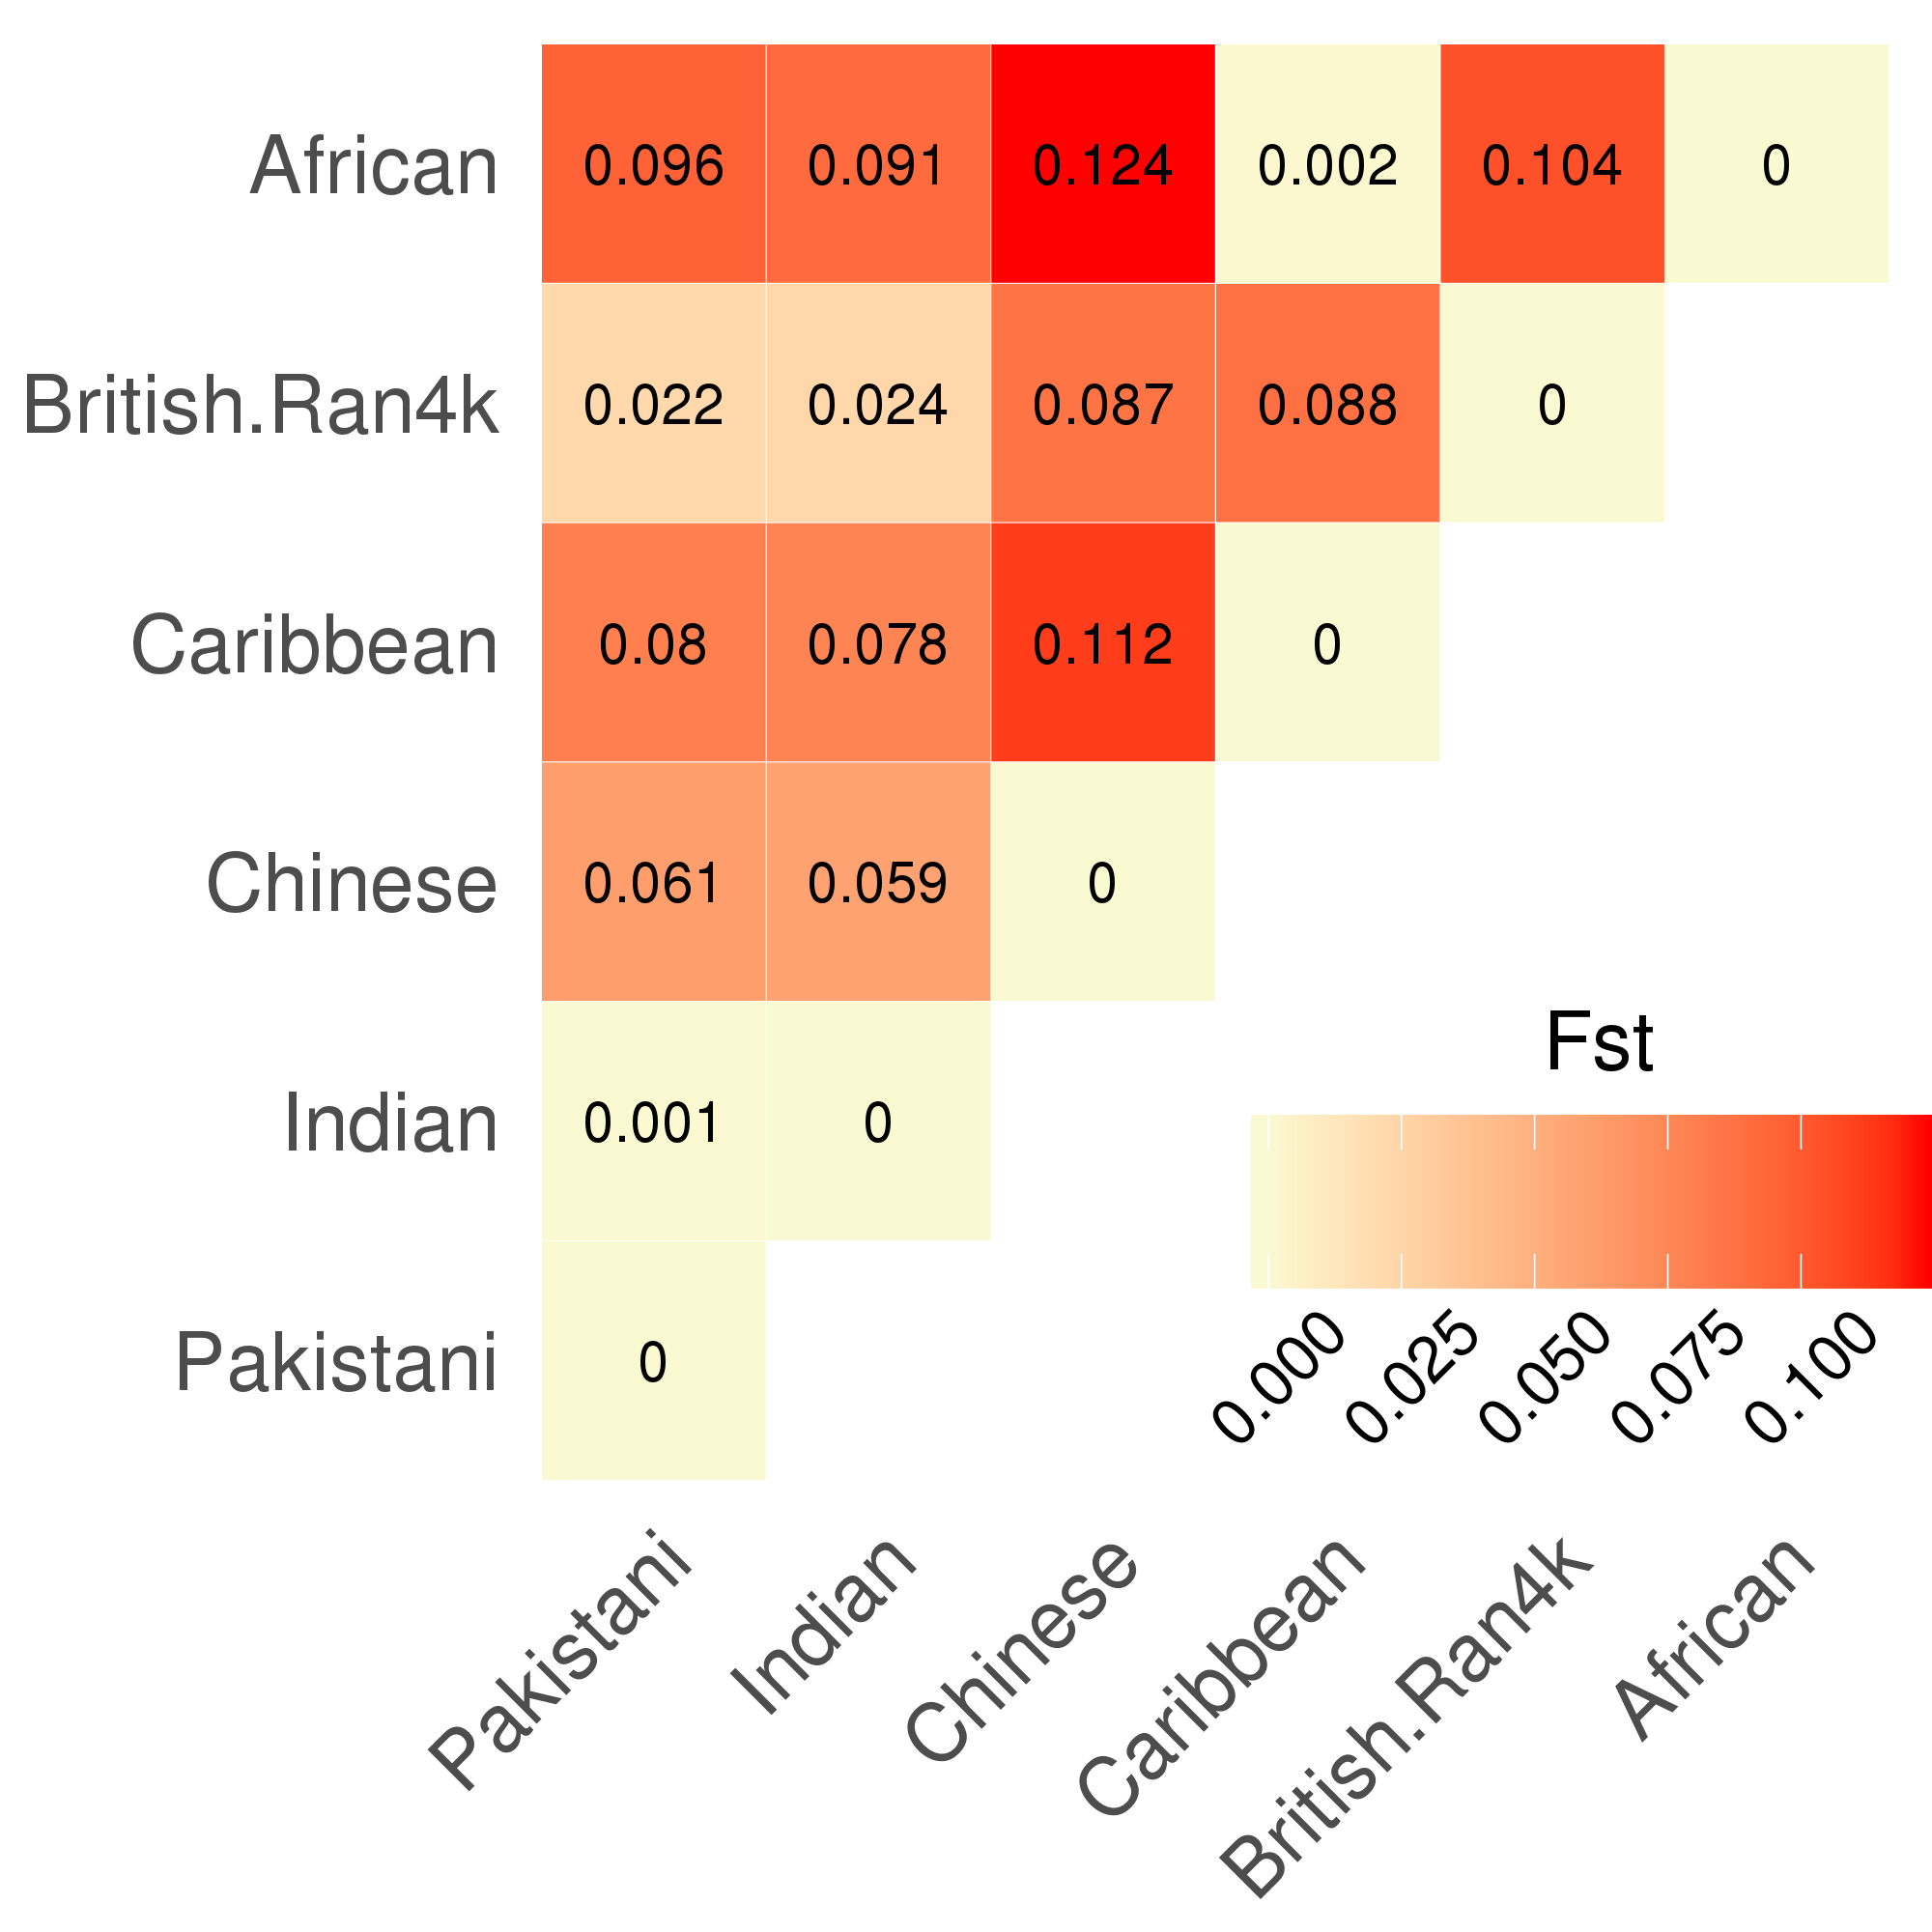
\includegraphics[scale=.5]{Images/Main/InterPath_Main_Figure_Fst_vs2.png}
%\caption[TBD]{\textbf{Distribution of pairwise F\textsubscript{ST} across the UKB subgroups}. The heatplot shows pairwise F\textsubscript{ST} values between each of our UKB population subgroups using our genome-wide SNP data. F\textsubscript{ST} values range from .001 to .124, and we observe typical global patterns (eg African and Caribbean being more differentiated versus non-African subgroups, Chinese being more differentiated versus non-Asian subgroups). These global patterns, however, do not match the distribution of total number of significant MAPIT-R pathways observed per-ancestry in Figure \ref{InterPath-Main-Figure-Barplots-KEGG} and Supplementary Figure \ref{InterPath-Supp-Figure-Barplots-REACTOME}.}
%\label{InterPath-Main-Figure-Fst}
%\end{figure}

%\begin{figure}[htb]
%\centering
%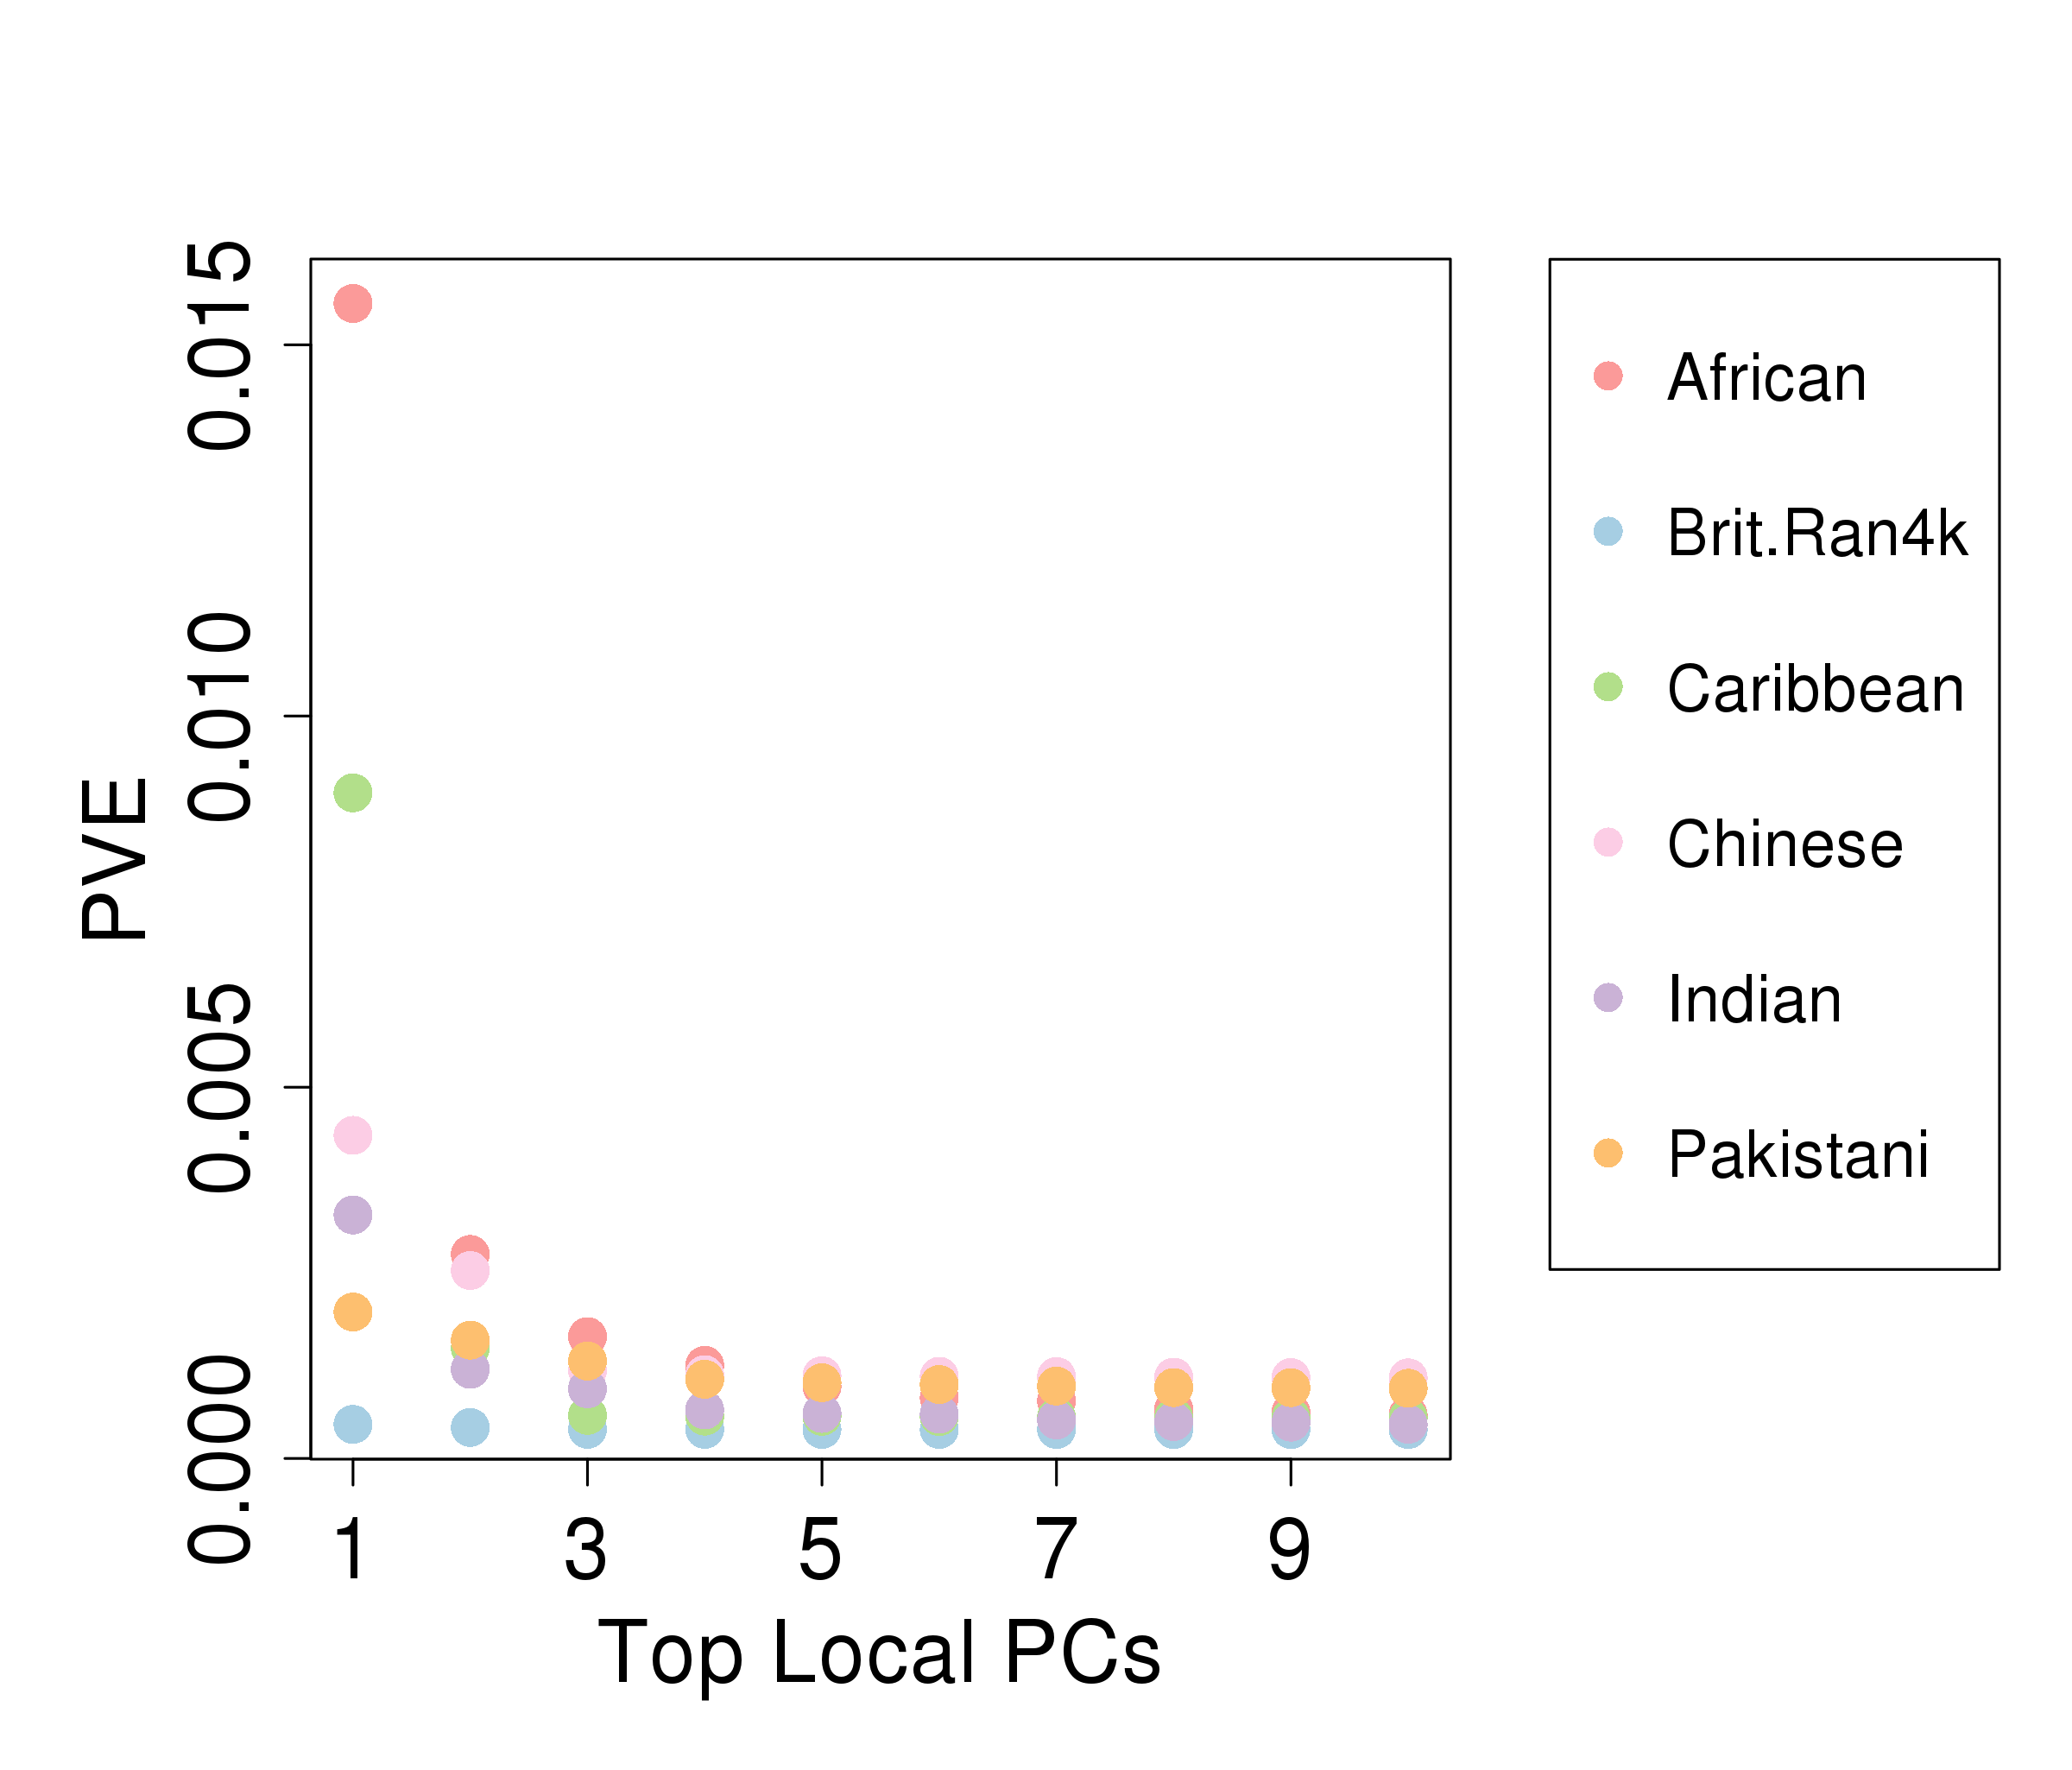
\includegraphics[scale=.5]{Images/Main/InterPath_Main_Figure_Eigenvalues_vs2.png}
%\caption[TBD]{\textbf{Distribution of top 10 local principal component PVEs across UKB subgroups}. The plot shows the PVE of each of the top 10 local PCs for each of our UKB population subgroups. Local here continues to refer to calculating PCs within each subgroup separately (versus calculating PCs jointly across all subgroups together). We observe that the distribution of PC1 PVEs among our subgroups appears to strongly correlate with the distribution of total number of genome-wide significant MAPIT-R pathways we identify per subgroup (see Figure \ref{InterPath-Main-Figure-Barplots-KEGG} and  Supplementary Figure \ref{InterPath-Supp-Figure-Barplots-REACTOME}).}
%\label{InterPath-Main-Figure-Eigenvalues}
%\end{figure}

To take these analyses one step further, we investigated levels of genetic diversity on the pathway-scale as well to see if they are correlated with the MAPIT-R results. To accomplish this, we calculated the mean proportion of pairwise identity-by-state across every pair of individuals on the pathway level. Meaning for a single pathway, we had a metric ranging from 0 to 1 where 1 indicates all pairs of individuals had exactly the same genotypes at every SNP for a given pathway and 0 means all pairs of individuals had completely different genotypes at each of these SNPs. Lower values would then indicate greater levels of genetic diversity for a given pathway within that ancestry subgroup. Once we had these values, we then compared them against each pathway's MAPIT-R -$\log_{10}$ $p$-value; however, we found there was no relationship between these two metrics (Figure \ref{InterPath-Main-Figure-IBS-African} \& Supplementary Figure \ref{InterPath-Supp-Figure-IBS-AllPops}). This was true across almost every combination of phenotype, pathway database, and UKB subgroup. And in directly comparing population subgroups against one another, it can be seen that the per-pathway IBS proportions follow similar trajectories, shifted only by each population's mean level of IBS (Figure \ref{InterPath-Main-Figure-IBS-AllPopComps-KEGG} \& Supplementary Figure \ref{InterPath-Supp-Figure-IBS-AllPopComps-REACTOME}). Therefore it appears this further supports our previous finding that the signal we are observing in our results is likely not being driven by broadscale levels of genetic variation. Instead, there may be a more cryptic structure and relationship between the genetic variation in each subgroup and the power to detect epistasis we are observing with MAPIT-R.

%\begin{figure}[htb]
%\centering
%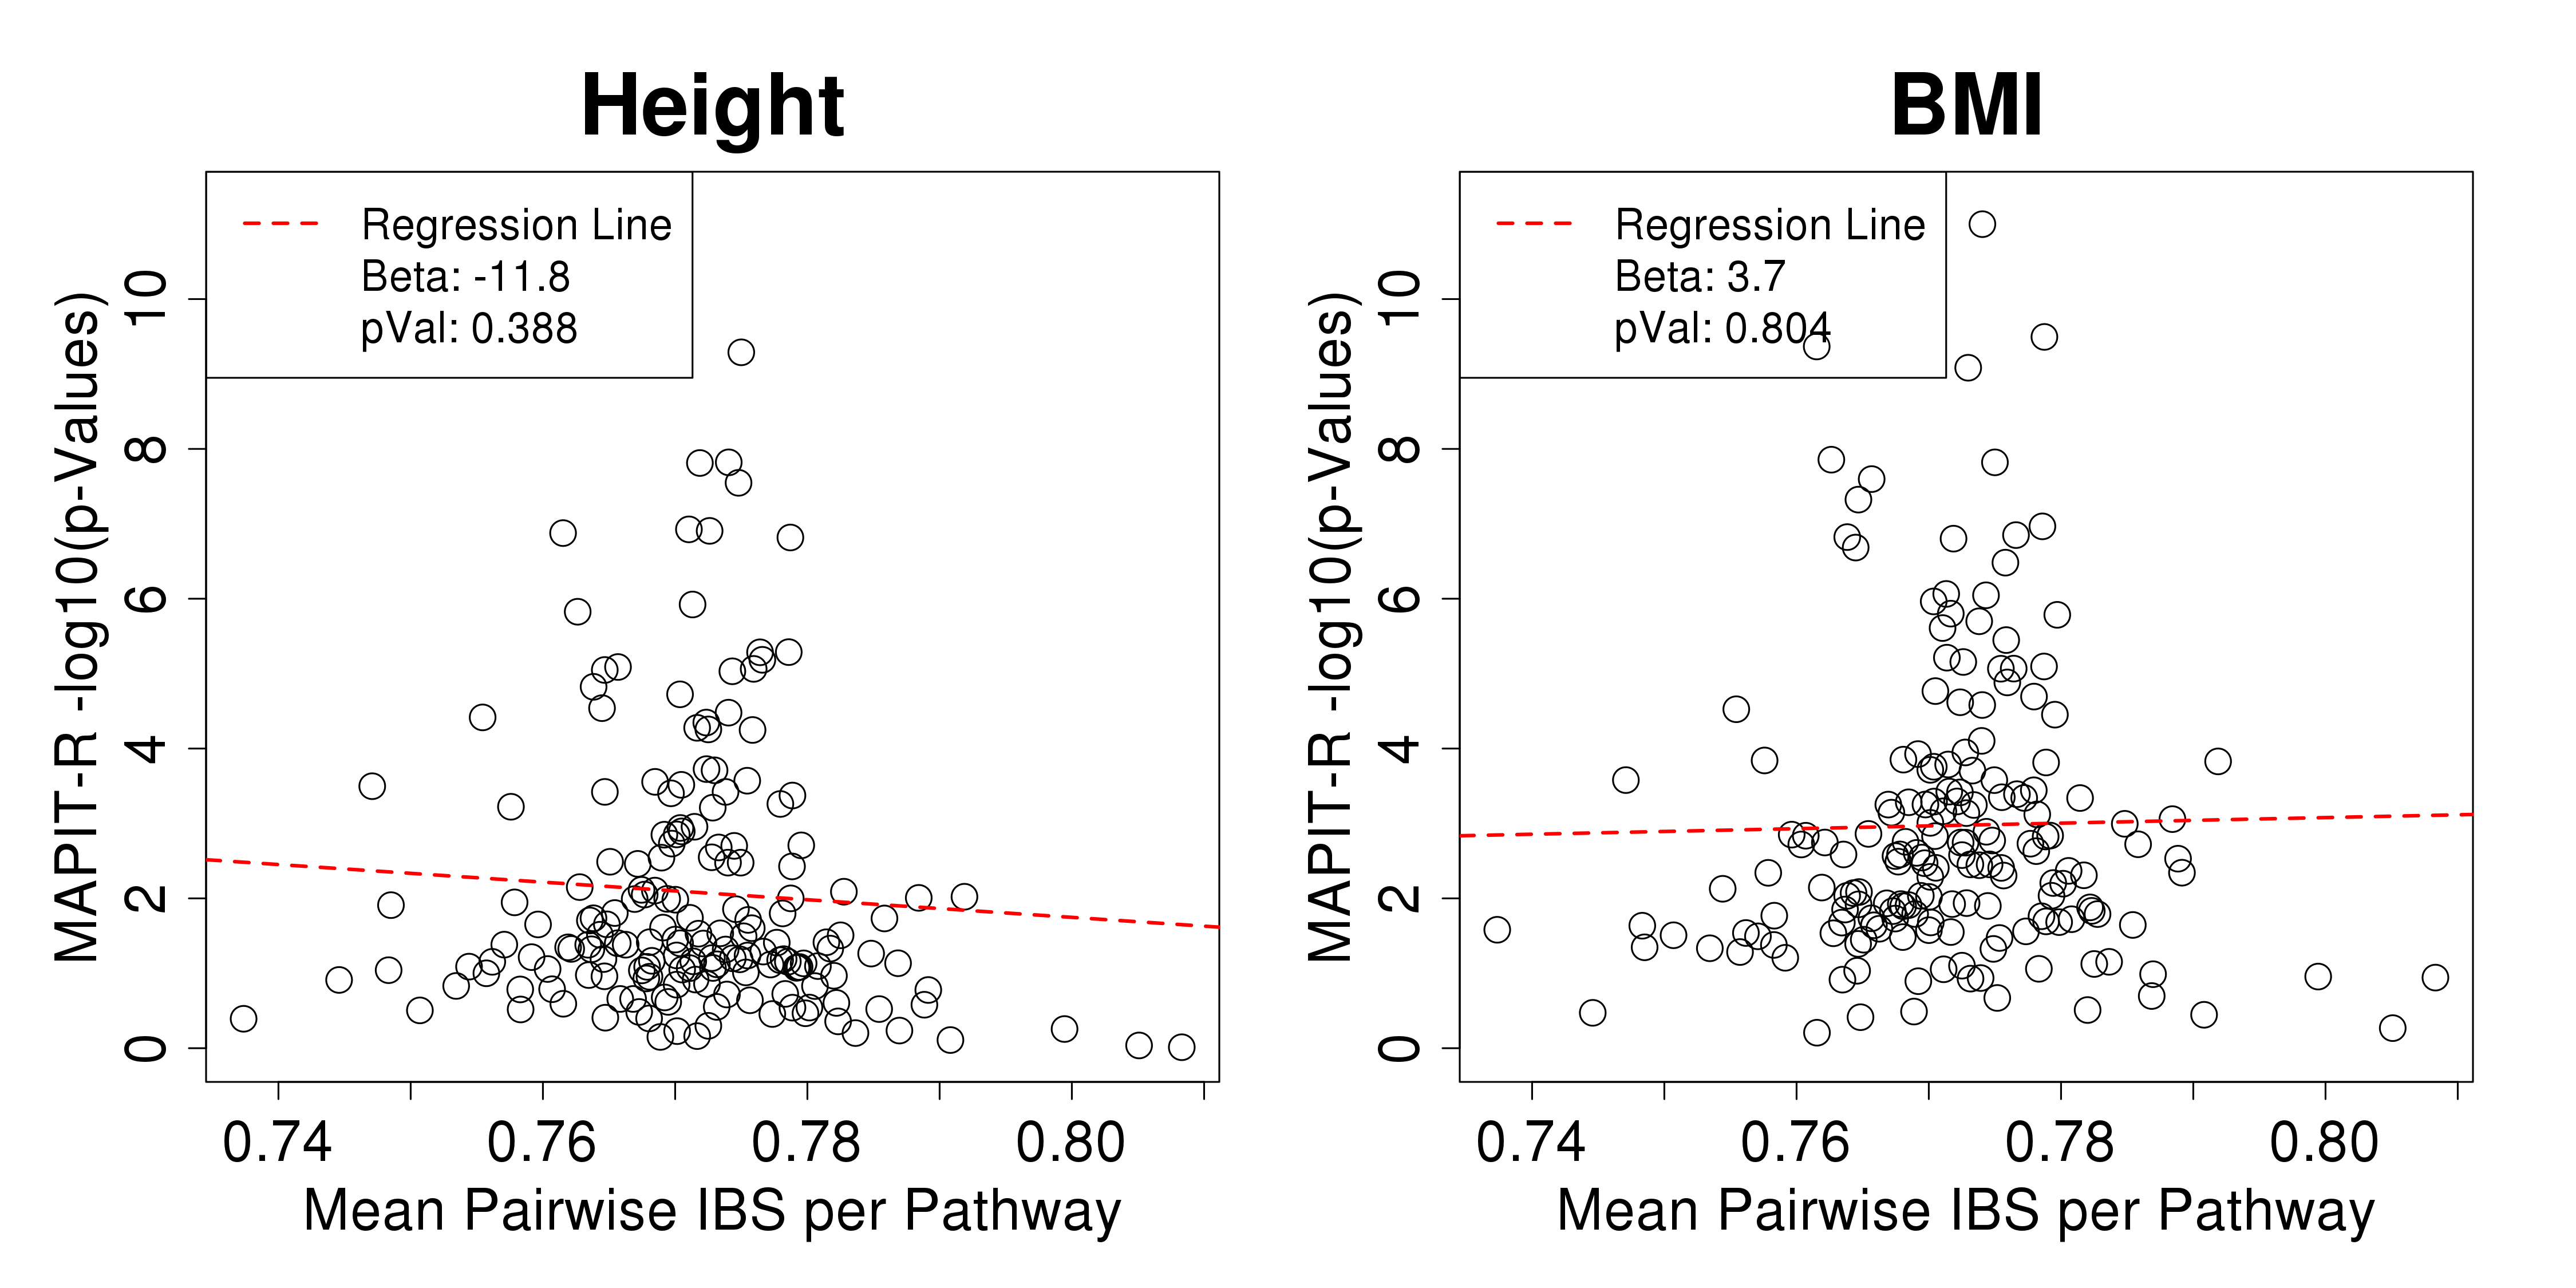
\includegraphics[scale=.35]{Images/Main/InterPath_Main_Figure_IBS_vs3_African.png}
%\caption[TBD]{\textbf{Pathway-level genetic diversity versus MAPIT-R results in the African subgroup and KEGG database}. The figure shows the mean pairwise IBS proportions per pathway plotted against each pathway's MAPIT-R $p$-value for the African subgroup KEGG height and BMI analysis. IBS proportions were calculated per pathway by using each pathway's set of SNPs to derive pairwise IBS values between every set of individuals in the subgroup, and then averaging across each of these pairs for a final summary metric. Results for each phenotype, database, and subgroup combination can be found in Supplementary Figure \ref{InterPath-Supp-Figure-IBS-AllPops}. We observe across almost every combination no significant relationship between a pathway's mean pairwise IBS proportion and its MAPIT-R $p$-value.}
%\label{InterPath-Main-Figure-IBS-African}
%\end{figure}

%\begin{figure}[htb]
%\centering
%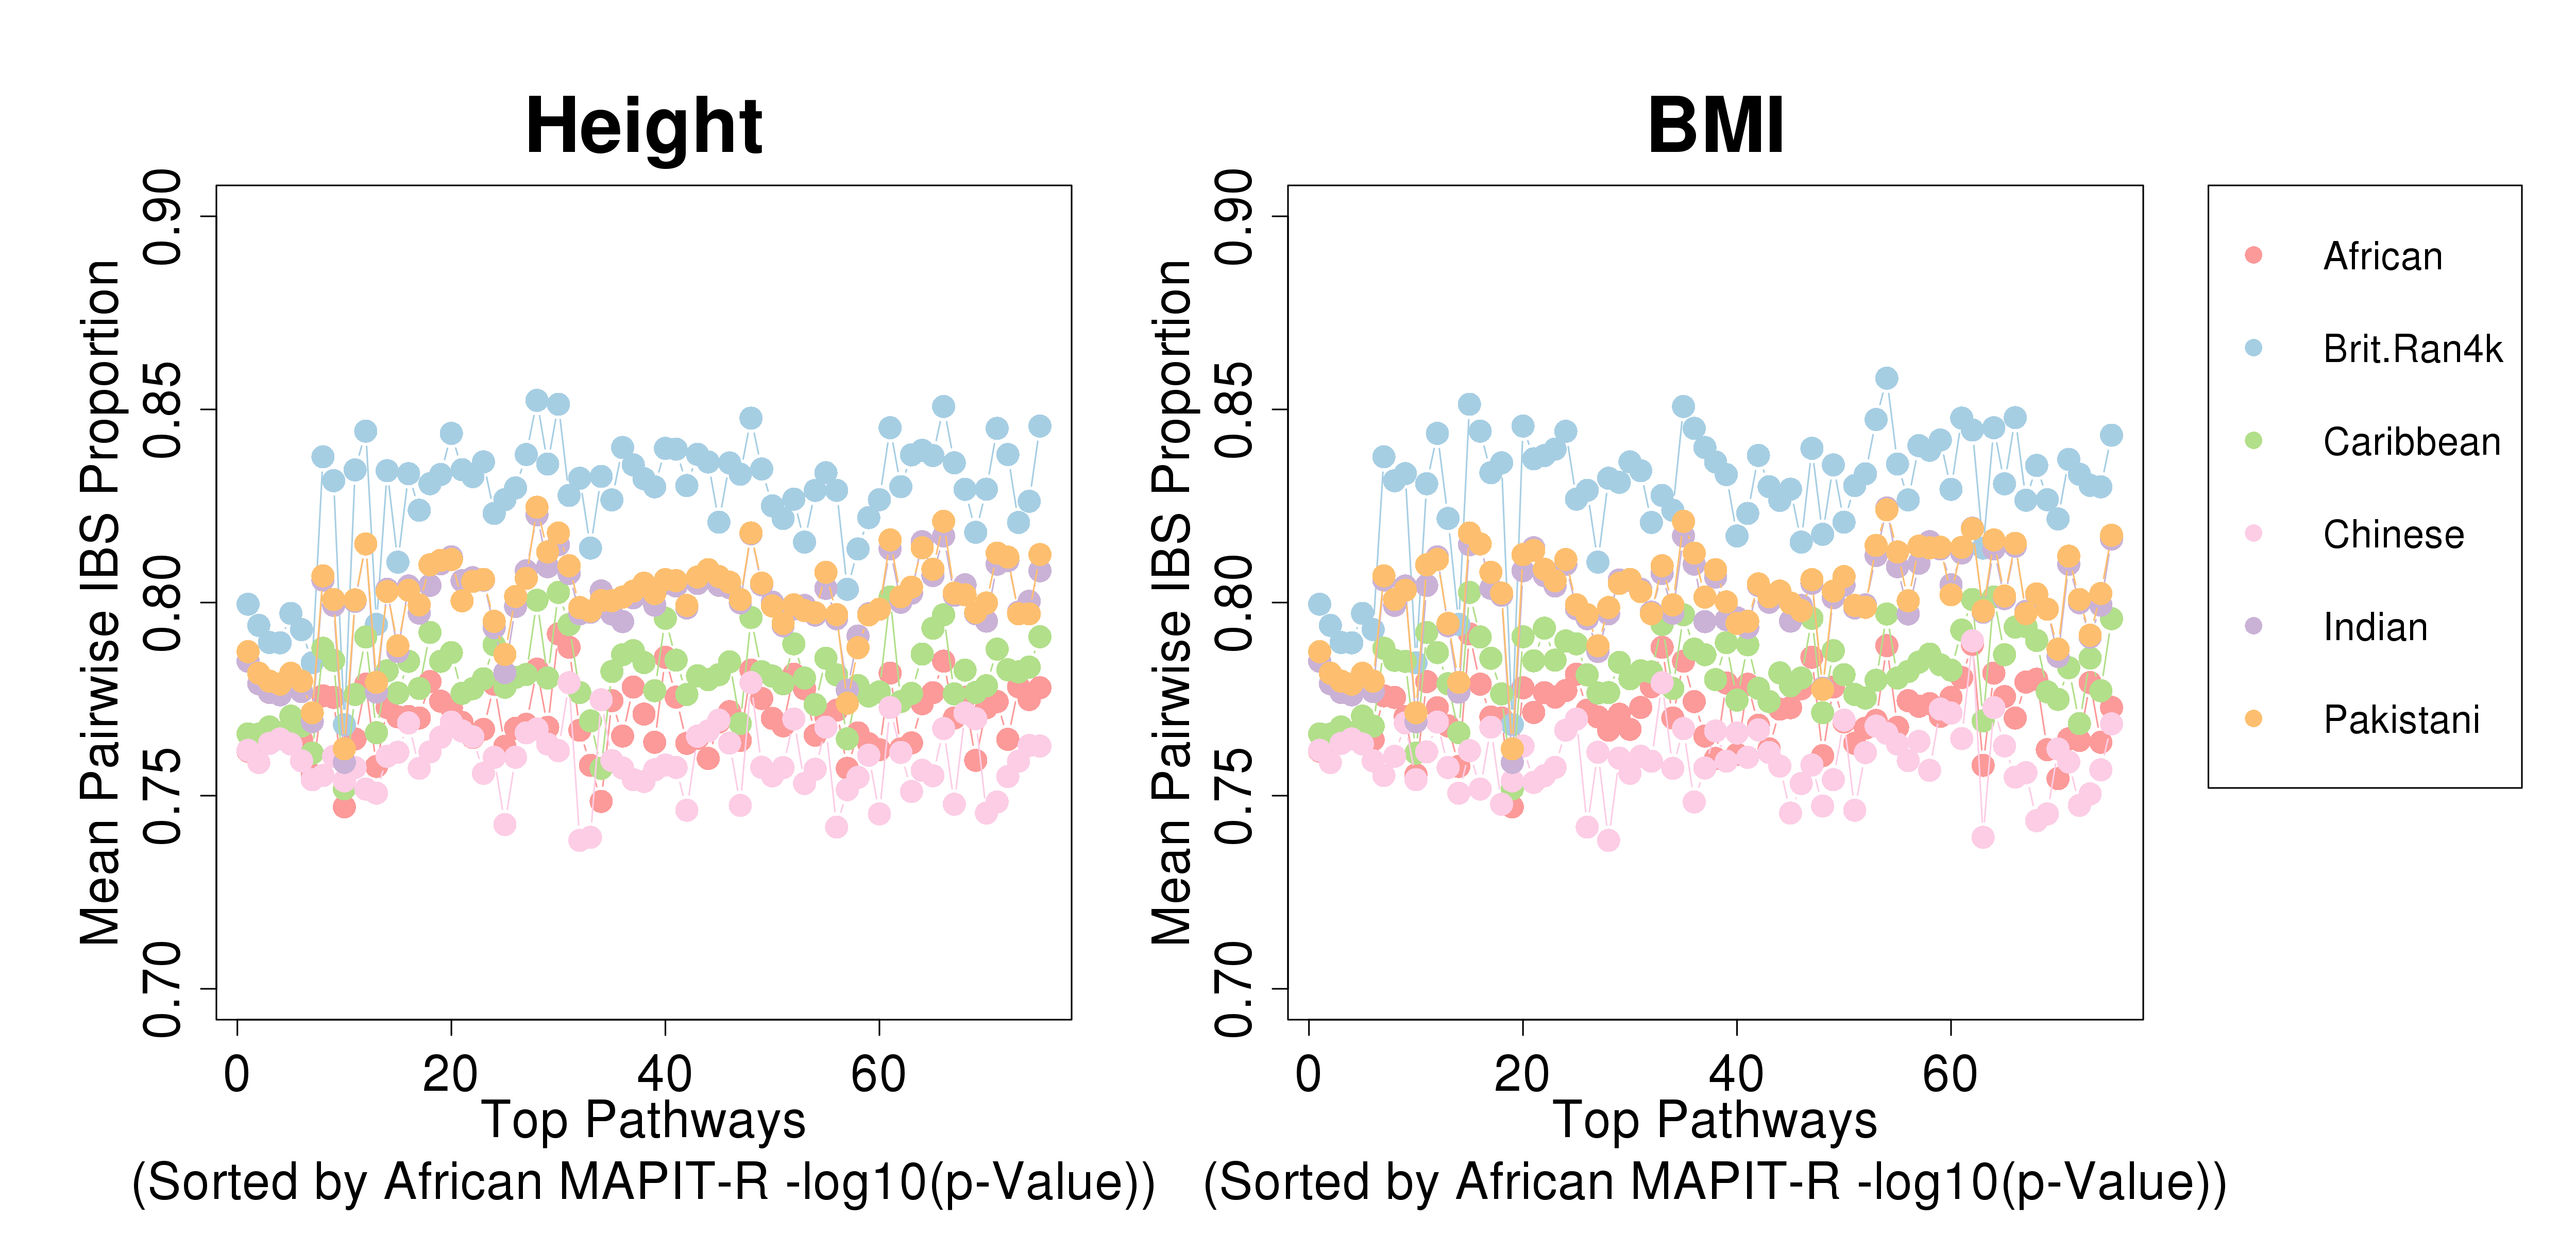
\includegraphics[scale=.35]{Images/Main/InterPath_Main_Figure_IBS_AllPopComps_vs3_KEGG.png}
%\caption[TBD]{\textbf{Pathway-level genetic diversity across all UKB subgroups for top African MAPIT-R KEGG pathways}. The figure plots the mean pairwise IBS proportions of each UKB subgroup for the top 75 KEGG pathways (sorted by MAPIT-R African subgroup $p$-value). Mean pairwise IBS proportions appear to follow similar trajectories across each subgroup, shifted mainly by average mean pairwise IBS proportion differences between subgroups. Results for both phenotypes in the REACTOME database can be see in Supplementary Figure %\ref{InterPath-Supp-Figure-IBS-AllPopComps-REACTOME}.}
%\label{InterPath-Main-Figure-IBS-AllPopComps-KEGG}
%\end{figure}










\fi

\end{document}
